% 高一74_宜川中学_10月月考.tex
%   —— 高一上数学“2026-2027 年宜川中学高一上 10 月月考”（讲评版）
% 试卷版：xelatex 高一74_宜川中学_10月月考.tex
% 答案版：xelatex "\def\isanswer{1}% 高一74_宜川中学_10月月考.tex
%   —— 高一上数学“2026-2027 年宜川中学高一上 10 月月考”（讲评版）
% 试卷版：xelatex 高一74_宜川中学_10月月考.tex
% 答案版：xelatex "\def\isanswer{1}% 高一74_宜川中学_10月月考.tex
%   —— 高一上数学“2026-2027 年宜川中学高一上 10 月月考”（讲评版）
% 试卷版：xelatex 高一74_宜川中学_10月月考.tex
% 答案版：xelatex "\def\isanswer{1}% 高一74_宜川中学_10月月考.tex
%   —— 高一上数学“2026-2027 年宜川中学高一上 10 月月考”（讲评版）
% 试卷版：xelatex 高一74_宜川中学_10月月考.tex
% 答案版：xelatex "\def\isanswer{1}\input{高一74_宜川中学_10月月考.tex}"
% 紧凑版：xelatex "\def\iscompact{1}\input{高一74_宜川中学_10月月考.tex}"
%
% 原始材料：微信公众号“魔都数学加油站”文章，连载“27学年高一74”；
% 原文标题“27学年高一74——2026-2027年上海市宜川中学高一上10月月考”；
% 原文链接：https://mp.weixin.qq.com/s/ymsl2bmkBRY6ZPDiUFCDTA。
% 页面标注发布时间 2026-10-22 21:45（上海）。
% 正文为 9 张 PNG 页（`原图/高一74_宜川中学_10月月考/01..09.png`）：
% 第 1、2、3 页为 4762×6735，其余 6 页为 2560×3620，均按页序读取。
% 9 页全为试卷正文页（卷首标题在第 1 页页顶，卷末第 18 题 (3) 解析止于第 9 页），
% 无封面页、目录页、二维码或宣传页。粉色斜排“魔都数学加油站”为卷面水印，未录入。
%
% 卷首标题：照卷面印作“2026-2027 年宜川中学高一上 10 月月考”（黑体加粗一行）。
% 原卷年份区间用半角连字符，本稿按全稿惯例排 en dash；原卷无副标题。
%
% 篇幅与题号：原卷自第 3 题起编号（第 1、2 题不在本卷内）。填空题 3—10（8 题）、
% 选择题 11—14（4 题）、解答题 15—18（4 题），共 16 题。本稿沿用原节与原题号，
% 只改排为全稿统一的大节样式。
%
% 讲评版：原卷第 3 题只印【答案】（“{(1,1)}”），本稿只给 \ans{}；其余 15 题均印
% 【解析】，用 \solbegin…\solend。四道选择题的作答括号原卷即留空，答案写在解析末句
% “故选 A／B／B／D”，照录在解析内，不另提 \ans{}。
%
% 副标题：原卷未印副标题。本稿按“知识模块”口径标作“集合与常用逻辑用语、不等式”：
% 16 题中集合与常用逻辑用语 7 题（第 3、9、10、15、16、18 题及第 17 题的反证法），
% 不等式 9 题（第 4—8、11—14、17 题），两类均确有分量，故并标。口径同 高一63、高一68—73。
%
% 与原卷的排版差异：
%   ① 原卷每题下直接印【答案】/【解析】，本稿按全稿惯例将答案与解析置于答案版；
%   ② 原卷未印副标题，本稿按“知识模块”口径补出；
%   ③ 原卷填空横线约四个字宽，本稿按全稿惯例统一排 \blankline[4.4em]；
%   ④ 原卷数集记号排斜体 $R$、$Z$、$N$（第 8、9、10、14—18 题），本稿按全稿惯例
%      改用 $\R$、$\Z$、$\N$（同 高一68—73）；第 18 题的正整数集合作 $\N^*$，照录；
%   ⑤ 原卷句末标点多为西文句点，均逐处照录；
%   ⑥ 第 15—18 题的子问原卷印作“（1）…（2）…”，本稿按 高一69—73 成例用行内
%      “（1）（2）（3）”段，解析中的子问标号用 \stepm{(1)}{…}；
%   ⑦ 每道解答题原卷未留作答空白，本稿按全稿惯例加 \ansspace（末题用 \ansspace*）；
%   ⑧ 选择题的作答括号原卷排半角“(    )”，本稿按全稿惯例排 \mbox{（\quad）}；
%      选项行排照原卷——第 11、13 题一行四条，第 12、14 题一行四条；
%   ⑨ 第 9、14、18 题解析中的不等式组／方程组，原卷均排作“{”连接的多行式，
%      本稿按全稿惯例排 cases；
%   ⑩ 第 8 题解析有一幅数轴图：原卷印在【解析】第 2 行之后，题干无“如图”二字。
%      本稿按原卷截图裁取（`figures/gao74_q8_numline.png`，由第 2 页原图裁出、
%      去除粉色水印后转灰度，未放大），放在答案版解析第 2 条之后；
%   ⑪ 第 18 题 (3) 解析中有一张 5 列 6 行的枚举表（原卷无表头、左侧两列留空以表示
%      沿用上格的 $A_4$／$A_5$），本稿照原卷排成同样的空格表，未加表头、未合并单元格。
%
% 原卷笔误/存疑（均照录未改，正文对应处另有 % 注）：
%   ① 第 14 题题干“维修费前 $x(x\in N)$ 年共 $\dfrac{25}{36}x^2+2x$ 千元”中的
%      $N$ 原卷排斜体，按全稿惯例改 $\N$，含义不变；
%   ② 第 18 题 (3) 的枚举表第 1—3 行与第 4—6 行分属“$A_5(1,4)$”“$A_5(1,3)$”两种
%      情形，原卷只在首行重复写 $A_4$、$A_5$，其余留空；本稿照录留空，未补字。
%
% 行数核对：逐题数 \step/\stepm 条数与原卷【解析】印刷行数，15 题逐一相符，
% 合计 104 条 / 104 行（Q4：1；Q5：2；Q6：3；Q7：3；Q8：3；Q9：3；Q10：15；
% Q11：2；Q12：3；Q13：3；Q14：4；Q15：9；Q16：6；Q17：10；Q18：37）。
% 另第 3 题只印【答案】，提 \ans{}，不计入 \step 账。
%
% 插图：第 8 题解析的数轴图，见上⑩；全卷题干无其他配图。
%
\documentclass[a4paper,11pt]{article}
\usepackage{common}

\begin{document}

\examtitlest[3]{2026--2027 年宜川中学高一上 10 月月考}{集合与常用逻辑用语、不等式}

\bigsec{一、填空题}

\begin{enumerate}
\setcounter{enumi}{2}

\item 已知集合 $A=\{(x,y)\mid y=x\}$，集合 $B=\{(x,y)\mid y=2-x\}$，则 $A\cap B=$\blankline[4.4em].

\ifanswer
\ans{$\{(1,1)\}$}
\fi

\item 已知 $a=\log_3 2$，$b=\log_3 8$，则 $3^{2a-b}=$\blankline[4.4em].

\ifanswer
\solbegin
\step{由 $a=\log_3 2$，$b=\log_3 8$，得 $3^a=2$，$3^b=8$，则 $3^{2a-b}=\dfrac{(3^a)^2}{3^b}=\dfrac48=\dfrac12$.}
\solend
\fi

\item 已知等式 $2x^2+3x+5=a(2x+1)(x+1)+c$ 恒成立，则实数 $c=$\blankline[4.4em].

\ifanswer
\solbegin
\step{$2x^2+3x+5=a(2x+1)(x+1)+c=2ax^2+3ax+a+c$，}
\step{则 $\begin{cases}2a=2\\ 3a=3\\ a+c=5\end{cases}$，解得 $c=4$.}
\solend
\fi

\item 已知 $x>0$，$y>0$，且 $\dfrac9x+\dfrac1y=1$，则 $x\cdot y$ 的最小值是\blankline[4.4em].

\ifanswer
\solbegin
\step{$x>0$，$y>0$，且 $1=\dfrac9x+\dfrac1y\geqslant2\sqrt{\dfrac9{xy}}$，}
\step{当且仅当 $x=9y$，即 $y=2$，$x=18$ 时取等号，所以 $xy\geqslant36$，}
\step{则 $x\cdot y$ 的最小值为 $36$.}
\solend
\fi

\item 已知关于 $x$ 的不等式 $x^2+bx+c>0$（$b$、$c$ 为实数）的解集为 $(-\infty,-2)\cup(3,+\infty)$，则不等式 $cx^2-bx+1\leqslant0$ 的解集为\blankline[4.4em].

\ifanswer
\solbegin
\step{由已知得 $-2$、$3$ 为方程 $x^2+bx+c=0$ 的根，所以 $-2+3=-b$，$-2\times3=c$，}
\step{即 $b=-1$，$c=-6$，所以不等式 $cx^2-bx+1\leqslant0$ 可变形为 $-6x^2+x+1\leqslant0$，}
\step{即 $6x^2-x-1\geqslant0$，解得 $x\leqslant-\dfrac13$ 或 $x\geqslant\dfrac12$，所以解集为 $\left(-\infty,-\dfrac13\right]\cup\left[\dfrac12,+\infty\right)$.}
\solend
\fi

\item 设 $x\in\R$，则方程 $|x-2|+|\sqrt\pi-x|=2-\sqrt\pi$ 的解集为\blankline[4.4em].

\ifanswer
\solbegin
\step{因为方程 $|x-2|+|\sqrt\pi-x|=2-\sqrt\pi$ 可化为 $|x-2|+|x-\sqrt\pi|=2-\sqrt\pi$，}
\needvspace{8\baselineskip}
\step{其表示数轴上实数 $x$ 到 $\sqrt\pi$ 与 $2$ 的距离之和等于 $2-\sqrt\pi$，如图：}
\begin{center}
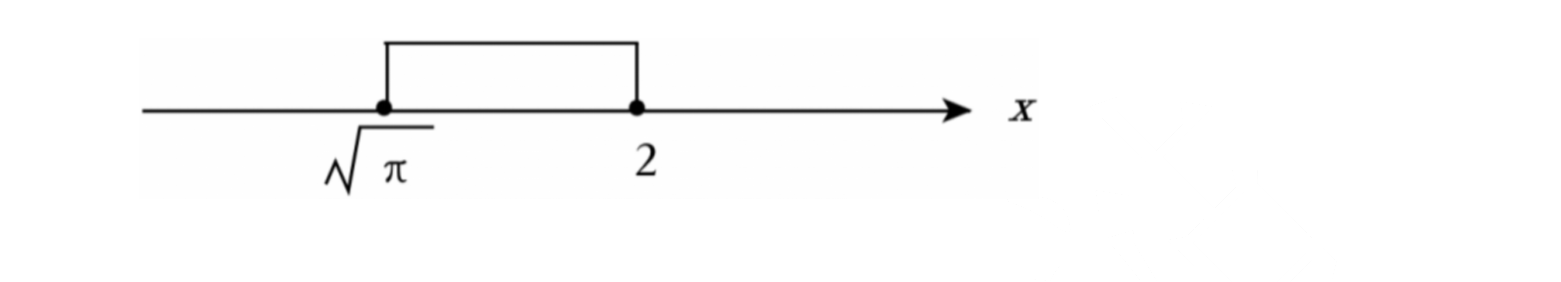
\includegraphics[width=0.72\textwidth]{figures/gao74_q8_numline.png}
\end{center}
\step{所以数形结合得所求集为 $[\sqrt\pi,2]$.}
\solend
\fi

\item 已知集合 $A=\{x\mid(a-1)x^2+3x-3=0,\,x\in\R\}$ 有且仅有一个真子集，则实数 $a=$\blankline[4.4em].

\ifanswer
\solbegin
\step{因为集合 $A=\{x\mid(a-1)x^2+3x-3=0,\,x\in\R\}$ 有且仅有一个真子集，}
\step{所以 $(a-1)x^2+3x-3=0$ 只有一个解，}
\step{所以 $a=1$ 或 $\begin{cases}a\neq1\\ \Delta=3^2-4(a-1)\times(-3)=0\end{cases}$，解得 $a=1$ 或 $a=\dfrac14$.}
\solend
\fi

\item 已知全集 $U=\{(x,y)\mid x,y\in\R\}$，若集合 $A\subseteq U$，且对任意 $(x_1,y_1)\in A$，均存在 $(x_2,y_2)\in A$，使得 $x_1y_2+x_2y_1=0$，则称集合 $A$ 为“对称对点集”. 给出如下集合：

（1）$A=\{(x,y)\mid x,y\in\Z\}$；

（2）$A=\left\{(x,y)\,\middle|\,y=\begin{cases}x+1,&x\geqslant0\\ -x+1,&x<0\end{cases},\ x\in\R,\ x\neq0\right\}$；

（3）$A=\{(x,y)\mid y=x+2,\,x\in\R\}$；

（4）$A=\left\{(x,y)\,\middle|\,y=\dfrac1x,\ x\in\R,\ x\neq0\right\}$.

其中是“对称对点集”的序号为\blankline[4.4em]（写出所有正确的序号）.

\ifanswer
\solbegin
\stepm{(1)}{因为 $0\in\Z$，所以 $(0,0)\in A$.}
\step{对任意 $(x_1,y_1)\in A$，取 $(x_2,y_2)=(0,0)\in A$，}
\step{都有 $x_1\times0+0\times y_1=0$，所以（1）是对称对点集.}
\stepm{(2)}{当 $x_1>0$ 时 $y_1=x_1+1$，取 $x_2=-x_1<0$、$y_2=-x_2+1=x_1+1=y_1$，}
\step{则 $(x_2,y_2)\in A$，且 $x_1y_2+x_2y_1=x_1y_1-x_1y_1=0$；}
\step{当 $x_1<0$ 时同理取 $x_2=-x_1>0$、$y_2=x_2+1=y_1$，}
\step{也有 $(x_2,y_2)\in A$ 且 $x_1y_2+x_2y_1=0$；所以（2）是对称对点集.}
\stepm{(3)}{取 $A$ 中的点 $(-1,1)$. 若存在 $(x_2,y_2)\in A$ 使 $(-1)\cdot y_2+x_2\cdot1=0$，}
\step{则 $y_2=x_2$，但 $A$ 中点的坐标满足 $y=x+2$，两者矛盾，}
\step{所以（3）不是对称对点集.}
\stepm{(4)}{设 $(x_1,y_1)\in A$，则 $x_1\neq0$ 且 $y_1=\dfrac1{x_1}$，}
\step{若存在 $(x_2,y_2)\in A$ 使 $x_1y_2+x_2y_1=0$，}
\step{把 $y_1=\dfrac1{x_1}$、$y_2=\dfrac1{x_2}$（$x_2\neq0$）代入得 $\dfrac{x_1}{x_2}+\dfrac{x_2}{x_1}=0$，即 $x_1^2+x_2^2=0$，}
\step{于是 $x_1=x_2=0$，与 $x_1\neq0$、$x_2\neq0$ 矛盾，所以（4）不是对称对点集.}
\step{故正确的是①②.}
\solend
\fi

\end{enumerate}

\bigsec{二、选择题}

\begin{enumerate}
\setcounter{enumi}{10}

\item “$x>3$”是“$\dfrac{x-1}{x-3}>0$”的\mbox{（\quad）}

\keepwithprev
A. 充分不必要条件\qquad B. 必要不充分条件\qquad C. 充要条件\qquad D. 既不充分也不必要条件

\ifanswer
\solbegin
\step{由 $\dfrac{x-1}{x-3}>0$ 得 $x>3$ 或 $x<1$，故“$x>3$”是“$\dfrac{x-1}{x-3}>0$”的充分不必要条件.}
\step{故选 $A$.}
\solend
\fi

\item 已知 $a,b,c\in\R$，$b>c$，则下列不等式中恒成立的是\mbox{（\quad）}

\keepwithprev
A. $a+b^2>a+c^2$\qquad B. $a^2+b>a^2+c$\qquad C. $ab^2>ac^2$\qquad D. $a^2b>a^2c$

\ifanswer
\solbegin
\step{对于 $A$，取 $b=1,c=-1$，错误；对于 $B$，由不等式的同向可加性得正确；}
\step{对于 $C$，取 $a=1,b=1,c=-2$，错误；对于 $D$，取 $a=0$，错误.}
\step{故选 $B$.}
\solend
\fi

\item 已知关于 $x$ 的不等式 $x^2-2kx+1>0$ 对于一切实数 $x$ 都成立，则实数 $k$ 的取值范围是\mbox{（\quad）}

\keepwithprev
A. $[-1,1]$\qquad B. $(-1,1)$\qquad C. $(-\infty,-1)\cup(1,+\infty)$\qquad D. $\left(-\dfrac12,\dfrac12\right)$

\ifanswer
\solbegin
\step{因为关于 $x$ 的不等式 $x^2-2kx+1>0$ 对于一切实数 $x$ 都成立，}
\step{所以 $\Delta=(-2k)^2-4<0$，即 $4k^2-4<0$，解得 $-1<k<1$，}
\step{所以实数 $k$ 的取值范围是 $(-1,1)$. 故选 $B$.}
\solend
\fi

\item 某种生产设备购买时费用 $100$ 千元，每年的设备管理费 $8$ 千元，这种生产设备的维修费前 $x(x\in\N)$ 年共 $\dfrac{25}{36}x^2+2x$ 千元，问这种生产设备最多使用\mbox{（\quad）}年报废最合算？（即年平均费用最少）

\keepwithprev
A. $13$\qquad B. $10$\qquad C. $15$\qquad D. $12$

\ifanswer
\solbegin
\step{设使用 $x$ 年报废，则总费用 $S(x)=100+8x+\dfrac{25}{36}x^2+2x=\dfrac{25}{36}x^2+10x+100$，}
\step{则年平均费用为 $y=\dfrac{S(x)}x=\dfrac{25x}{36}+\dfrac{100}x+10\geqslant2\sqrt{\dfrac{25x}{36}\cdot\dfrac{100}x}+10=\dfrac{80}3$，}
\step{当且仅当 $\dfrac{25x}{36}=\dfrac{100}x$，即 $x=12$ 时，取等号，}
\step{故当使用 $12$ 年报废，年平均费用最少. 故选 $D$.}
\solend
\fi

\end{enumerate}

\bigsec{三、解答题}

\begin{enumerate}
\setcounter{enumi}{14}

\item （1）设集合 $A=\{x\mid ax-1=0,\,x\in\R\}$，$B=\{x\mid x^2-3x+2=0,\,x\in\R\}$，若 $A\cap B\neq\varnothing$，求实数 $a$ 的取值范围；

（2）已知一元二次方程 $x^2-mx+m+1=0$ 的两个不等实根为 $x_1$、$x_2$，且 $x_1^2+x_2^2=1$，求实数 $m$ 的值.

\ifanswer
\solbegin
\stepm{(1)}{$B=\{x\mid x^2-3x+2=0,\,x\in\R\}=\{1,2\}$，}
\step{①当 $a=0$ 时，方程 $0\cdot x-1=0$ 无解，$A=\varnothing$，$A\cap B=\varnothing$，不符合题意；}
\step{②当 $a\neq0$ 时，$A=\left\{\dfrac1a\right\}$. $A\cap B\neq\varnothing$，}
\step{则 $\dfrac1a\in B$，即 $\dfrac1a=1$ 或 $\dfrac1a=2$，解得 $a=1$ 或 $\dfrac12$；}
\stepm{(2)}{方程 $x^2-mx+m+1=0$ 有两个不等实根，}
\step{则 $\Delta=m^2-4(m+1)>0$，解得 $m>2+2\sqrt2$ 或 $m<2-2\sqrt2$，}
\step{由韦达定理得 $x_1+x_2=m$，$x_1x_2=m+1$，$x_1^2+x_2^2=1$，}
\step{则 $(x_1+x_2)^2-2x_1x_2=m^2-2(m+1)=1$，解得 $m=-1$ 或 $m=3$（舍去），}
\step{综上所述，$m=-1$.}
\solend
\fi

\ansspace

\item 设全集为 $\R$，已知集合 $A=\{x\mid|x-1|\leqslant3,\,x\in\R\}$，

$B=\{x\mid x^2-2mx+(m-3)(m+3)\leqslant0,\,x\in\R\}$.

（1）若 $A\cap B=[0,4]$，求实数 $m$ 的值；

（2）若 $A\cap\overline{B}=A$，求实数 $m$ 的取值范围.

\ifanswer
\solbegin
\stepm{(1)}{$A=\{x\mid|x-1|\leqslant3\}=\{x\mid-2\leqslant x\leqslant4\}$，}
\step{$B=\{x\mid x^2-2mx+(m-3)(m+3)\leqslant0\}=\{x\mid m-3\leqslant x\leqslant m+3\}$，}
\step{若 $A\cap B=[0,4]$，则 $m-3=0$，即 $m=3$；}
\stepm{(2)}{若 $A\cap\overline{B}=A$，则 $A\subseteq\overline{B}$，$\overline{B}=\{x\mid x>m+3\text{ 或 }x<m-3\}$，}
\step{所以 $m+3<-2$ 或 $m-3>4$，解得 $m<-5$ 或 $m>7$，}
\step{实数 $m$ 的取值范围为 $\{m\mid m<-5\text{ 或 }m>7\}$.}
\solend
\fi

\ansspace

\item （1）已知 $a$、$b$ 为正实数，若 $a+b>4$，试用反证法证明：$\dfrac{a}{b+2}$ 和 $\dfrac{b}{a+2}$ 中至少有一个\mbox{大于 $\dfrac12$}；

（2）设 $x$、$y$ 为正实数，$m=\sqrt{2x}+\sqrt{2y}$，$n=\sqrt{x^2+5xy+y^2}$，试比较 $m$、$n$ 的大小，并说明理由.

\ifanswer
\solbegin
\stepm{(1)}{假设 $\dfrac{a}{b+2}\leqslant\dfrac12$ 且 $\dfrac{b}{a+2}\leqslant\dfrac12$，}
\step{又由 $a$、$b$ 为正实数，则有 $2a\leqslant b+2$ 且 $2b\leqslant a+2$，}
\step{两式相加，有 $2a+2b\leqslant a+b+4$，变形得 $a+b\leqslant4$，}
\step{与已知 $a+b>4$ 相矛盾，即假设 $\dfrac{a}{b+2}\leqslant\dfrac12$ 且 $\dfrac{b}{a+2}\leqslant\dfrac12$ 不成立，}
\step{故 $\dfrac{a}{b+2}$ 和 $\dfrac{b}{a+2}$ 中至少有一个\mbox{大于 $\dfrac12$}；}
\stepm{(2)}{$m>n$，理由：$x$、$y$ 为正实数，$m=\sqrt{2x}+\sqrt{2y}$，$n=\sqrt{x^2+5xy+y^2}$，}
\step{则 $m^2=(\sqrt{2x}+\sqrt{2y})^2=2x^2+2y^2+4xy$，$n^2=x^2+y^2+5xy$，}
\step{则有 $m^2-n^2=2x^2+2y^2+4xy-x^2-y^2-5xy=x^2+y^2-xy$}
\step{$=\left(x-\dfrac y2\right)^2+\dfrac{3y^2}4$，}
\step{又 $x$、$y$ 为正实数，则 $m^2-n^2>0$，即 $m^2>n^2$，必有 $m>n$，结论成立.}
\solend
\fi

\ansspace

\item 已知集合 $A=\{a_1,a_2,a_3,\cdots,a_n\}$，$a_i$ 为正整数（$i=1,2,\cdots,n$）.

（1）设 $n=3$，$a_1=1$，$a_2=3$，$a_3=9$，$B=\{a_i+a_j\mid1\leqslant i<j\leqslant3,\,i,j\in\N^*\}$，若互不相同的三个实数 $b_1$、$b_2$、$b_3$，满足 $\{b_i+b_j\mid1\leqslant i<j\leqslant3,\,i,j\in\N^*\}=B$，求有序数组 $(b_1,b_2,b_3)$；

（2）设 $n=4$，$C=\{a_1^2,a_2^2,a_3^2,a_4^2\}$，其中 $a_1<a_2<a_3<a_4$，$A\cap C=\{a_1,a_4\}$，且 $a_1+a_4=10$，$A\cup C$ 中所有元素之和为 $124$，求集合 $A$；

（3）设 $n=2$，有 $7$ 个互不相同的集合 $A$ 分别记为 $A_1$、$A_2$、$A_3$、$\cdots$、$A_7$，且 $A_1\cap A_7=\varnothing$、$A_i\cap A_{i+1}=\varnothing\,(i=1,2,3,\cdots,6)$，记 $D=A_1\cup A_2\cup A_3\cup\cdots\cup A_7$，求 $D$ 中元素个数的最小值.

\ifanswer
\solbegin
\stepm{(1)}{$B=\{a_i+a_j\mid1\leqslant i<j\leqslant3,\,i,j\in\N^*\}=\{1+3,1+9,3+9\}=\{4,10,12\}$，}
\step{由题意，不妨设 $b_1<b_2<b_3$，}
\step{则三个数两两之和为 $\begin{cases}b_1+b_2=4\\ b_1+b_3=10\\ b_2+b_3=12\end{cases}$，解得 $\begin{cases}b_1=1\\ b_2=3\\ b_3=9\end{cases}$，}
\step{所以满足条件的有序数组为 $1$，$3$，$9$ 三个数字的全部排列，}
\step{所以有序数组 $(b_1,b_2,b_3)$ 为 $(1,3,9),(1,9,3),(3,1,9),(3,9,1),(9,1,3),(9,3,1)$；}
\stepm{(2)}{因为 $A\cap C=\{a_1,a_4\}$，所以 $a_1\in C$，$a_4\in C$，}
\step{所以 $a_1$ 是集合 $A$ 中某个正整数的平方，}
\step{又因为 $a_1$ 是最小的正整数，所以只能是 $a_1=1$，此时满足 $1=1^2$.}
\step{又 $a_1+a_4=10$，所以 $a_4=9$，所以 $9$ 也是集合 $A$ 中某个正整数的平方，}
\step{因为 $3^2=9$，所以 $3\in A$，则有 $a_2=3$ 或 $a_3=3$.}
\step{若 $a_3=3$，则 $A=\{1,a_2,3,9\}$，$C=\{1^2,a_2^2,3^2,9^2\}=\{1,a_2^2,9,81\}$，}
\step{因为 $a_1<a_2<a_3<a_4$，且 $a_2$ 为正整数，所以只能是 $a_2=2$，}
\step{故 $A=\{1,2,3,9\}$，$C=\{1,4,9,81\}$，$A\cap C=\{1,9\}$，符合题意，}
\step{则 $A\cup C=\{1,2,3,4,9,81\}$，此时 $1+2+3+4+9+81=100\neq124$，}
\step{故 $a_3=3$ 不符合题意，所以只能 $a_2=3$，}
\step{故 $A=\{1,3,a_3,9\}$，$C=\{1^2,3^2,a_3^2,9^2\}$，此时 $A\cup C=\{1,3,a_3,9,a_3^2,81\}$，}
\step{则有 $1+3+a_3+9+a_3^2+81=124$，}
\step{即 $a_3^2+a_3-30=(a_3+6)(a_3-5)=0$，解得正整数 $a_3=5$，}
\step{此时 $A=\{1,3,5,9\}$，$C=\{1,9,25,81\}$，$A\cup C=\{1,3,5,9,25,81\}$，}
\step{满足 $A\cap C=\{1,9\}$，$A\cup C$ 中所有元素之和为 $1+3+5+9+25+81=124$，}
\step{故 $A=\{1,3,5,9\}$；}
\stepm{(3)}{当 $n=2$ 时，每个集合 $A_i(i=1,2,\cdots,7)$ 均为含有 $2$ 个元素的二元集合，}
\step{设 $D$ 中元素个数为 $m$，}
\step{若 $m\leqslant4$，从 $m$ 个元素中最多能得到 $\dfrac{4\times3}2=6$ 个不同二元集合，不足 $7$ 个，}
\step{故 $m\leqslant4$ 不可能.}
\step{若 $m=5$，则有 $\dfrac{5\times4}2=10$ 个不同二元集合，数量超过 $7$ 个，符合要求.}
\step{因为 $A_i\cap A_{i+1}=\varnothing(i=1,2,3,\cdots,6)$，$A_1\cap A_7=\varnothing$，}
\step{即要求 $7$ 个互不相同的二元集合排成环，}
\step{且相邻（含首尾）集合交集为空集.}
\needvspace{12\baselineskip}
\step{假设 $m=5$，不妨设 $A_1(1,2)$、$A_2(3,4)$、$A_3(1,5)$，则：}
\begin{center}
\renewcommand{\arraystretch}{1.9}
\begin{tabular}{|c|c|c|c|c|}
\hline
$A_4(2,3)$ & $A_5(1,4)$ & $A_6(2,5)$ & $A_7(1,3)$ & 与 $A_1$ 矛盾\\
\hline
 &  & $A_6(3,5)$ & $A_7(2,4)$ & 与 $A_1$ 矛盾\\
\hline
 & $A_5(4,5)$ & $A_6(1,3)$ & $A_7(2,5)$ 或 $A_7(2,4)$ & 与 $A_1$ 矛盾\\
\hline
$A_4(2,4)$ & $A_5(1,3)$ & $A_6(2,5)$ & $A_7(1,4)$ & 与 $A_1$ 矛盾\\
\hline
 &  & $A_6(4,5)$ & $A_7(2,3)$ & 与 $A_1$ 矛盾\\
\hline
 & $A_5(3,5)$ & $A_6(1,4)$ & $A_7(2,3)$ 或 $A_7(2,5)$ & 与 $A_1$ 矛盾\\
\hline
\end{tabular}
\end{center}
\step{故 $m=5$ 不可能.}
\step{综上，$m\geqslant6$，取 $D=\{1,2,3,4,5,6\}$，}
\step{令 $A_1=\{1,2\},A_2=\{3,4\},A_3=\{1,5\},A_4=\{2,4\},A_5=\{3,6\},A_6=\{1,4\}$，}
\step{$A_7=\{5,6\}$，此时 $A_1$、$A_2$、$\cdots$、$A_7$ 是 $7$ 个互不相同的二元集合，}
\step{且 $A_1\cap A_2=\varnothing$，$A_2\cap A_3=\varnothing$，$A_3\cap A_4=\varnothing$，$A_4\cap A_5=\varnothing$，}
\step{$A_5\cap A_6=\varnothing$，$A_6\cap A_7=\varnothing$，$A_7\cap A_1=\varnothing$，满足全部条件，}
\step{故 $D$ 中元素个数的最小值为 $6$.}
\solend
\fi

\ansspace*[7]

\end{enumerate}

\end{document}
"
% 紧凑版：xelatex "\def\iscompact{1}% 高一74_宜川中学_10月月考.tex
%   —— 高一上数学“2026-2027 年宜川中学高一上 10 月月考”（讲评版）
% 试卷版：xelatex 高一74_宜川中学_10月月考.tex
% 答案版：xelatex "\def\isanswer{1}\input{高一74_宜川中学_10月月考.tex}"
% 紧凑版：xelatex "\def\iscompact{1}\input{高一74_宜川中学_10月月考.tex}"
%
% 原始材料：微信公众号“魔都数学加油站”文章，连载“27学年高一74”；
% 原文标题“27学年高一74——2026-2027年上海市宜川中学高一上10月月考”；
% 原文链接：https://mp.weixin.qq.com/s/ymsl2bmkBRY6ZPDiUFCDTA。
% 页面标注发布时间 2026-10-22 21:45（上海）。
% 正文为 9 张 PNG 页（`原图/高一74_宜川中学_10月月考/01..09.png`）：
% 第 1、2、3 页为 4762×6735，其余 6 页为 2560×3620，均按页序读取。
% 9 页全为试卷正文页（卷首标题在第 1 页页顶，卷末第 18 题 (3) 解析止于第 9 页），
% 无封面页、目录页、二维码或宣传页。粉色斜排“魔都数学加油站”为卷面水印，未录入。
%
% 卷首标题：照卷面印作“2026-2027 年宜川中学高一上 10 月月考”（黑体加粗一行）。
% 原卷年份区间用半角连字符，本稿按全稿惯例排 en dash；原卷无副标题。
%
% 篇幅与题号：原卷自第 3 题起编号（第 1、2 题不在本卷内）。填空题 3—10（8 题）、
% 选择题 11—14（4 题）、解答题 15—18（4 题），共 16 题。本稿沿用原节与原题号，
% 只改排为全稿统一的大节样式。
%
% 讲评版：原卷第 3 题只印【答案】（“{(1,1)}”），本稿只给 \ans{}；其余 15 题均印
% 【解析】，用 \solbegin…\solend。四道选择题的作答括号原卷即留空，答案写在解析末句
% “故选 A／B／B／D”，照录在解析内，不另提 \ans{}。
%
% 副标题：原卷未印副标题。本稿按“知识模块”口径标作“集合与常用逻辑用语、不等式”：
% 16 题中集合与常用逻辑用语 7 题（第 3、9、10、15、16、18 题及第 17 题的反证法），
% 不等式 9 题（第 4—8、11—14、17 题），两类均确有分量，故并标。口径同 高一63、高一68—73。
%
% 与原卷的排版差异：
%   ① 原卷每题下直接印【答案】/【解析】，本稿按全稿惯例将答案与解析置于答案版；
%   ② 原卷未印副标题，本稿按“知识模块”口径补出；
%   ③ 原卷填空横线约四个字宽，本稿按全稿惯例统一排 \blankline[4.4em]；
%   ④ 原卷数集记号排斜体 $R$、$Z$、$N$（第 8、9、10、14—18 题），本稿按全稿惯例
%      改用 $\R$、$\Z$、$\N$（同 高一68—73）；第 18 题的正整数集合作 $\N^*$，照录；
%   ⑤ 原卷句末标点多为西文句点，均逐处照录；
%   ⑥ 第 15—18 题的子问原卷印作“（1）…（2）…”，本稿按 高一69—73 成例用行内
%      “（1）（2）（3）”段，解析中的子问标号用 \stepm{(1)}{…}；
%   ⑦ 每道解答题原卷未留作答空白，本稿按全稿惯例加 \ansspace（末题用 \ansspace*）；
%   ⑧ 选择题的作答括号原卷排半角“(    )”，本稿按全稿惯例排 \mbox{（\quad）}；
%      选项行排照原卷——第 11、13 题一行四条，第 12、14 题一行四条；
%   ⑨ 第 9、14、18 题解析中的不等式组／方程组，原卷均排作“{”连接的多行式，
%      本稿按全稿惯例排 cases；
%   ⑩ 第 8 题解析有一幅数轴图：原卷印在【解析】第 2 行之后，题干无“如图”二字。
%      本稿按原卷截图裁取（`figures/gao74_q8_numline.png`，由第 2 页原图裁出、
%      去除粉色水印后转灰度，未放大），放在答案版解析第 2 条之后；
%   ⑪ 第 18 题 (3) 解析中有一张 5 列 6 行的枚举表（原卷无表头、左侧两列留空以表示
%      沿用上格的 $A_4$／$A_5$），本稿照原卷排成同样的空格表，未加表头、未合并单元格。
%
% 原卷笔误/存疑（均照录未改，正文对应处另有 % 注）：
%   ① 第 14 题题干“维修费前 $x(x\in N)$ 年共 $\dfrac{25}{36}x^2+2x$ 千元”中的
%      $N$ 原卷排斜体，按全稿惯例改 $\N$，含义不变；
%   ② 第 18 题 (3) 的枚举表第 1—3 行与第 4—6 行分属“$A_5(1,4)$”“$A_5(1,3)$”两种
%      情形，原卷只在首行重复写 $A_4$、$A_5$，其余留空；本稿照录留空，未补字。
%
% 行数核对：逐题数 \step/\stepm 条数与原卷【解析】印刷行数，15 题逐一相符，
% 合计 104 条 / 104 行（Q4：1；Q5：2；Q6：3；Q7：3；Q8：3；Q9：3；Q10：15；
% Q11：2；Q12：3；Q13：3；Q14：4；Q15：9；Q16：6；Q17：10；Q18：37）。
% 另第 3 题只印【答案】，提 \ans{}，不计入 \step 账。
%
% 插图：第 8 题解析的数轴图，见上⑩；全卷题干无其他配图。
%
\documentclass[a4paper,11pt]{article}
\usepackage{common}

\begin{document}

\examtitlest[3]{2026--2027 年宜川中学高一上 10 月月考}{集合与常用逻辑用语、不等式}

\bigsec{一、填空题}

\begin{enumerate}
\setcounter{enumi}{2}

\item 已知集合 $A=\{(x,y)\mid y=x\}$，集合 $B=\{(x,y)\mid y=2-x\}$，则 $A\cap B=$\blankline[4.4em].

\ifanswer
\ans{$\{(1,1)\}$}
\fi

\item 已知 $a=\log_3 2$，$b=\log_3 8$，则 $3^{2a-b}=$\blankline[4.4em].

\ifanswer
\solbegin
\step{由 $a=\log_3 2$，$b=\log_3 8$，得 $3^a=2$，$3^b=8$，则 $3^{2a-b}=\dfrac{(3^a)^2}{3^b}=\dfrac48=\dfrac12$.}
\solend
\fi

\item 已知等式 $2x^2+3x+5=a(2x+1)(x+1)+c$ 恒成立，则实数 $c=$\blankline[4.4em].

\ifanswer
\solbegin
\step{$2x^2+3x+5=a(2x+1)(x+1)+c=2ax^2+3ax+a+c$，}
\step{则 $\begin{cases}2a=2\\ 3a=3\\ a+c=5\end{cases}$，解得 $c=4$.}
\solend
\fi

\item 已知 $x>0$，$y>0$，且 $\dfrac9x+\dfrac1y=1$，则 $x\cdot y$ 的最小值是\blankline[4.4em].

\ifanswer
\solbegin
\step{$x>0$，$y>0$，且 $1=\dfrac9x+\dfrac1y\geqslant2\sqrt{\dfrac9{xy}}$，}
\step{当且仅当 $x=9y$，即 $y=2$，$x=18$ 时取等号，所以 $xy\geqslant36$，}
\step{则 $x\cdot y$ 的最小值为 $36$.}
\solend
\fi

\item 已知关于 $x$ 的不等式 $x^2+bx+c>0$（$b$、$c$ 为实数）的解集为 $(-\infty,-2)\cup(3,+\infty)$，则不等式 $cx^2-bx+1\leqslant0$ 的解集为\blankline[4.4em].

\ifanswer
\solbegin
\step{由已知得 $-2$、$3$ 为方程 $x^2+bx+c=0$ 的根，所以 $-2+3=-b$，$-2\times3=c$，}
\step{即 $b=-1$，$c=-6$，所以不等式 $cx^2-bx+1\leqslant0$ 可变形为 $-6x^2+x+1\leqslant0$，}
\step{即 $6x^2-x-1\geqslant0$，解得 $x\leqslant-\dfrac13$ 或 $x\geqslant\dfrac12$，所以解集为 $\left(-\infty,-\dfrac13\right]\cup\left[\dfrac12,+\infty\right)$.}
\solend
\fi

\item 设 $x\in\R$，则方程 $|x-2|+|\sqrt\pi-x|=2-\sqrt\pi$ 的解集为\blankline[4.4em].

\ifanswer
\solbegin
\step{因为方程 $|x-2|+|\sqrt\pi-x|=2-\sqrt\pi$ 可化为 $|x-2|+|x-\sqrt\pi|=2-\sqrt\pi$，}
\needvspace{8\baselineskip}
\step{其表示数轴上实数 $x$ 到 $\sqrt\pi$ 与 $2$ 的距离之和等于 $2-\sqrt\pi$，如图：}
\begin{center}
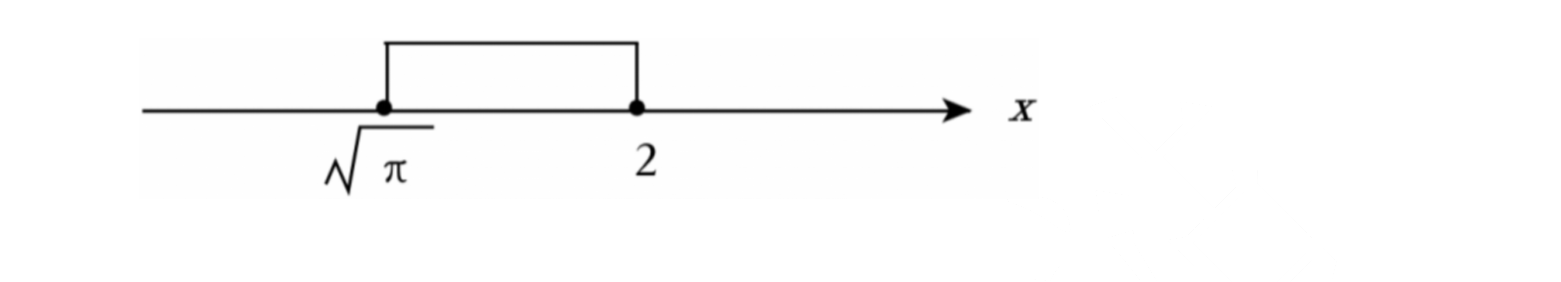
\includegraphics[width=0.72\textwidth]{figures/gao74_q8_numline.png}
\end{center}
\step{所以数形结合得所求集为 $[\sqrt\pi,2]$.}
\solend
\fi

\item 已知集合 $A=\{x\mid(a-1)x^2+3x-3=0,\,x\in\R\}$ 有且仅有一个真子集，则实数 $a=$\blankline[4.4em].

\ifanswer
\solbegin
\step{因为集合 $A=\{x\mid(a-1)x^2+3x-3=0,\,x\in\R\}$ 有且仅有一个真子集，}
\step{所以 $(a-1)x^2+3x-3=0$ 只有一个解，}
\step{所以 $a=1$ 或 $\begin{cases}a\neq1\\ \Delta=3^2-4(a-1)\times(-3)=0\end{cases}$，解得 $a=1$ 或 $a=\dfrac14$.}
\solend
\fi

\item 已知全集 $U=\{(x,y)\mid x,y\in\R\}$，若集合 $A\subseteq U$，且对任意 $(x_1,y_1)\in A$，均存在 $(x_2,y_2)\in A$，使得 $x_1y_2+x_2y_1=0$，则称集合 $A$ 为“对称对点集”. 给出如下集合：

（1）$A=\{(x,y)\mid x,y\in\Z\}$；

（2）$A=\left\{(x,y)\,\middle|\,y=\begin{cases}x+1,&x\geqslant0\\ -x+1,&x<0\end{cases},\ x\in\R,\ x\neq0\right\}$；

（3）$A=\{(x,y)\mid y=x+2,\,x\in\R\}$；

（4）$A=\left\{(x,y)\,\middle|\,y=\dfrac1x,\ x\in\R,\ x\neq0\right\}$.

其中是“对称对点集”的序号为\blankline[4.4em]（写出所有正确的序号）.

\ifanswer
\solbegin
\stepm{(1)}{因为 $0\in\Z$，所以 $(0,0)\in A$.}
\step{对任意 $(x_1,y_1)\in A$，取 $(x_2,y_2)=(0,0)\in A$，}
\step{都有 $x_1\times0+0\times y_1=0$，所以（1）是对称对点集.}
\stepm{(2)}{当 $x_1>0$ 时 $y_1=x_1+1$，取 $x_2=-x_1<0$、$y_2=-x_2+1=x_1+1=y_1$，}
\step{则 $(x_2,y_2)\in A$，且 $x_1y_2+x_2y_1=x_1y_1-x_1y_1=0$；}
\step{当 $x_1<0$ 时同理取 $x_2=-x_1>0$、$y_2=x_2+1=y_1$，}
\step{也有 $(x_2,y_2)\in A$ 且 $x_1y_2+x_2y_1=0$；所以（2）是对称对点集.}
\stepm{(3)}{取 $A$ 中的点 $(-1,1)$. 若存在 $(x_2,y_2)\in A$ 使 $(-1)\cdot y_2+x_2\cdot1=0$，}
\step{则 $y_2=x_2$，但 $A$ 中点的坐标满足 $y=x+2$，两者矛盾，}
\step{所以（3）不是对称对点集.}
\stepm{(4)}{设 $(x_1,y_1)\in A$，则 $x_1\neq0$ 且 $y_1=\dfrac1{x_1}$，}
\step{若存在 $(x_2,y_2)\in A$ 使 $x_1y_2+x_2y_1=0$，}
\step{把 $y_1=\dfrac1{x_1}$、$y_2=\dfrac1{x_2}$（$x_2\neq0$）代入得 $\dfrac{x_1}{x_2}+\dfrac{x_2}{x_1}=0$，即 $x_1^2+x_2^2=0$，}
\step{于是 $x_1=x_2=0$，与 $x_1\neq0$、$x_2\neq0$ 矛盾，所以（4）不是对称对点集.}
\step{故正确的是①②.}
\solend
\fi

\end{enumerate}

\bigsec{二、选择题}

\begin{enumerate}
\setcounter{enumi}{10}

\item “$x>3$”是“$\dfrac{x-1}{x-3}>0$”的\mbox{（\quad）}

\keepwithprev
A. 充分不必要条件\qquad B. 必要不充分条件\qquad C. 充要条件\qquad D. 既不充分也不必要条件

\ifanswer
\solbegin
\step{由 $\dfrac{x-1}{x-3}>0$ 得 $x>3$ 或 $x<1$，故“$x>3$”是“$\dfrac{x-1}{x-3}>0$”的充分不必要条件.}
\step{故选 $A$.}
\solend
\fi

\item 已知 $a,b,c\in\R$，$b>c$，则下列不等式中恒成立的是\mbox{（\quad）}

\keepwithprev
A. $a+b^2>a+c^2$\qquad B. $a^2+b>a^2+c$\qquad C. $ab^2>ac^2$\qquad D. $a^2b>a^2c$

\ifanswer
\solbegin
\step{对于 $A$，取 $b=1,c=-1$，错误；对于 $B$，由不等式的同向可加性得正确；}
\step{对于 $C$，取 $a=1,b=1,c=-2$，错误；对于 $D$，取 $a=0$，错误.}
\step{故选 $B$.}
\solend
\fi

\item 已知关于 $x$ 的不等式 $x^2-2kx+1>0$ 对于一切实数 $x$ 都成立，则实数 $k$ 的取值范围是\mbox{（\quad）}

\keepwithprev
A. $[-1,1]$\qquad B. $(-1,1)$\qquad C. $(-\infty,-1)\cup(1,+\infty)$\qquad D. $\left(-\dfrac12,\dfrac12\right)$

\ifanswer
\solbegin
\step{因为关于 $x$ 的不等式 $x^2-2kx+1>0$ 对于一切实数 $x$ 都成立，}
\step{所以 $\Delta=(-2k)^2-4<0$，即 $4k^2-4<0$，解得 $-1<k<1$，}
\step{所以实数 $k$ 的取值范围是 $(-1,1)$. 故选 $B$.}
\solend
\fi

\item 某种生产设备购买时费用 $100$ 千元，每年的设备管理费 $8$ 千元，这种生产设备的维修费前 $x(x\in\N)$ 年共 $\dfrac{25}{36}x^2+2x$ 千元，问这种生产设备最多使用\mbox{（\quad）}年报废最合算？（即年平均费用最少）

\keepwithprev
A. $13$\qquad B. $10$\qquad C. $15$\qquad D. $12$

\ifanswer
\solbegin
\step{设使用 $x$ 年报废，则总费用 $S(x)=100+8x+\dfrac{25}{36}x^2+2x=\dfrac{25}{36}x^2+10x+100$，}
\step{则年平均费用为 $y=\dfrac{S(x)}x=\dfrac{25x}{36}+\dfrac{100}x+10\geqslant2\sqrt{\dfrac{25x}{36}\cdot\dfrac{100}x}+10=\dfrac{80}3$，}
\step{当且仅当 $\dfrac{25x}{36}=\dfrac{100}x$，即 $x=12$ 时，取等号，}
\step{故当使用 $12$ 年报废，年平均费用最少. 故选 $D$.}
\solend
\fi

\end{enumerate}

\bigsec{三、解答题}

\begin{enumerate}
\setcounter{enumi}{14}

\item （1）设集合 $A=\{x\mid ax-1=0,\,x\in\R\}$，$B=\{x\mid x^2-3x+2=0,\,x\in\R\}$，若 $A\cap B\neq\varnothing$，求实数 $a$ 的取值范围；

（2）已知一元二次方程 $x^2-mx+m+1=0$ 的两个不等实根为 $x_1$、$x_2$，且 $x_1^2+x_2^2=1$，求实数 $m$ 的值.

\ifanswer
\solbegin
\stepm{(1)}{$B=\{x\mid x^2-3x+2=0,\,x\in\R\}=\{1,2\}$，}
\step{①当 $a=0$ 时，方程 $0\cdot x-1=0$ 无解，$A=\varnothing$，$A\cap B=\varnothing$，不符合题意；}
\step{②当 $a\neq0$ 时，$A=\left\{\dfrac1a\right\}$. $A\cap B\neq\varnothing$，}
\step{则 $\dfrac1a\in B$，即 $\dfrac1a=1$ 或 $\dfrac1a=2$，解得 $a=1$ 或 $\dfrac12$；}
\stepm{(2)}{方程 $x^2-mx+m+1=0$ 有两个不等实根，}
\step{则 $\Delta=m^2-4(m+1)>0$，解得 $m>2+2\sqrt2$ 或 $m<2-2\sqrt2$，}
\step{由韦达定理得 $x_1+x_2=m$，$x_1x_2=m+1$，$x_1^2+x_2^2=1$，}
\step{则 $(x_1+x_2)^2-2x_1x_2=m^2-2(m+1)=1$，解得 $m=-1$ 或 $m=3$（舍去），}
\step{综上所述，$m=-1$.}
\solend
\fi

\ansspace

\item 设全集为 $\R$，已知集合 $A=\{x\mid|x-1|\leqslant3,\,x\in\R\}$，

$B=\{x\mid x^2-2mx+(m-3)(m+3)\leqslant0,\,x\in\R\}$.

（1）若 $A\cap B=[0,4]$，求实数 $m$ 的值；

（2）若 $A\cap\overline{B}=A$，求实数 $m$ 的取值范围.

\ifanswer
\solbegin
\stepm{(1)}{$A=\{x\mid|x-1|\leqslant3\}=\{x\mid-2\leqslant x\leqslant4\}$，}
\step{$B=\{x\mid x^2-2mx+(m-3)(m+3)\leqslant0\}=\{x\mid m-3\leqslant x\leqslant m+3\}$，}
\step{若 $A\cap B=[0,4]$，则 $m-3=0$，即 $m=3$；}
\stepm{(2)}{若 $A\cap\overline{B}=A$，则 $A\subseteq\overline{B}$，$\overline{B}=\{x\mid x>m+3\text{ 或 }x<m-3\}$，}
\step{所以 $m+3<-2$ 或 $m-3>4$，解得 $m<-5$ 或 $m>7$，}
\step{实数 $m$ 的取值范围为 $\{m\mid m<-5\text{ 或 }m>7\}$.}
\solend
\fi

\ansspace

\item （1）已知 $a$、$b$ 为正实数，若 $a+b>4$，试用反证法证明：$\dfrac{a}{b+2}$ 和 $\dfrac{b}{a+2}$ 中至少有一个\mbox{大于 $\dfrac12$}；

（2）设 $x$、$y$ 为正实数，$m=\sqrt{2x}+\sqrt{2y}$，$n=\sqrt{x^2+5xy+y^2}$，试比较 $m$、$n$ 的大小，并说明理由.

\ifanswer
\solbegin
\stepm{(1)}{假设 $\dfrac{a}{b+2}\leqslant\dfrac12$ 且 $\dfrac{b}{a+2}\leqslant\dfrac12$，}
\step{又由 $a$、$b$ 为正实数，则有 $2a\leqslant b+2$ 且 $2b\leqslant a+2$，}
\step{两式相加，有 $2a+2b\leqslant a+b+4$，变形得 $a+b\leqslant4$，}
\step{与已知 $a+b>4$ 相矛盾，即假设 $\dfrac{a}{b+2}\leqslant\dfrac12$ 且 $\dfrac{b}{a+2}\leqslant\dfrac12$ 不成立，}
\step{故 $\dfrac{a}{b+2}$ 和 $\dfrac{b}{a+2}$ 中至少有一个\mbox{大于 $\dfrac12$}；}
\stepm{(2)}{$m>n$，理由：$x$、$y$ 为正实数，$m=\sqrt{2x}+\sqrt{2y}$，$n=\sqrt{x^2+5xy+y^2}$，}
\step{则 $m^2=(\sqrt{2x}+\sqrt{2y})^2=2x^2+2y^2+4xy$，$n^2=x^2+y^2+5xy$，}
\step{则有 $m^2-n^2=2x^2+2y^2+4xy-x^2-y^2-5xy=x^2+y^2-xy$}
\step{$=\left(x-\dfrac y2\right)^2+\dfrac{3y^2}4$，}
\step{又 $x$、$y$ 为正实数，则 $m^2-n^2>0$，即 $m^2>n^2$，必有 $m>n$，结论成立.}
\solend
\fi

\ansspace

\item 已知集合 $A=\{a_1,a_2,a_3,\cdots,a_n\}$，$a_i$ 为正整数（$i=1,2,\cdots,n$）.

（1）设 $n=3$，$a_1=1$，$a_2=3$，$a_3=9$，$B=\{a_i+a_j\mid1\leqslant i<j\leqslant3,\,i,j\in\N^*\}$，若互不相同的三个实数 $b_1$、$b_2$、$b_3$，满足 $\{b_i+b_j\mid1\leqslant i<j\leqslant3,\,i,j\in\N^*\}=B$，求有序数组 $(b_1,b_2,b_3)$；

（2）设 $n=4$，$C=\{a_1^2,a_2^2,a_3^2,a_4^2\}$，其中 $a_1<a_2<a_3<a_4$，$A\cap C=\{a_1,a_4\}$，且 $a_1+a_4=10$，$A\cup C$ 中所有元素之和为 $124$，求集合 $A$；

（3）设 $n=2$，有 $7$ 个互不相同的集合 $A$ 分别记为 $A_1$、$A_2$、$A_3$、$\cdots$、$A_7$，且 $A_1\cap A_7=\varnothing$、$A_i\cap A_{i+1}=\varnothing\,(i=1,2,3,\cdots,6)$，记 $D=A_1\cup A_2\cup A_3\cup\cdots\cup A_7$，求 $D$ 中元素个数的最小值.

\ifanswer
\solbegin
\stepm{(1)}{$B=\{a_i+a_j\mid1\leqslant i<j\leqslant3,\,i,j\in\N^*\}=\{1+3,1+9,3+9\}=\{4,10,12\}$，}
\step{由题意，不妨设 $b_1<b_2<b_3$，}
\step{则三个数两两之和为 $\begin{cases}b_1+b_2=4\\ b_1+b_3=10\\ b_2+b_3=12\end{cases}$，解得 $\begin{cases}b_1=1\\ b_2=3\\ b_3=9\end{cases}$，}
\step{所以满足条件的有序数组为 $1$，$3$，$9$ 三个数字的全部排列，}
\step{所以有序数组 $(b_1,b_2,b_3)$ 为 $(1,3,9),(1,9,3),(3,1,9),(3,9,1),(9,1,3),(9,3,1)$；}
\stepm{(2)}{因为 $A\cap C=\{a_1,a_4\}$，所以 $a_1\in C$，$a_4\in C$，}
\step{所以 $a_1$ 是集合 $A$ 中某个正整数的平方，}
\step{又因为 $a_1$ 是最小的正整数，所以只能是 $a_1=1$，此时满足 $1=1^2$.}
\step{又 $a_1+a_4=10$，所以 $a_4=9$，所以 $9$ 也是集合 $A$ 中某个正整数的平方，}
\step{因为 $3^2=9$，所以 $3\in A$，则有 $a_2=3$ 或 $a_3=3$.}
\step{若 $a_3=3$，则 $A=\{1,a_2,3,9\}$，$C=\{1^2,a_2^2,3^2,9^2\}=\{1,a_2^2,9,81\}$，}
\step{因为 $a_1<a_2<a_3<a_4$，且 $a_2$ 为正整数，所以只能是 $a_2=2$，}
\step{故 $A=\{1,2,3,9\}$，$C=\{1,4,9,81\}$，$A\cap C=\{1,9\}$，符合题意，}
\step{则 $A\cup C=\{1,2,3,4,9,81\}$，此时 $1+2+3+4+9+81=100\neq124$，}
\step{故 $a_3=3$ 不符合题意，所以只能 $a_2=3$，}
\step{故 $A=\{1,3,a_3,9\}$，$C=\{1^2,3^2,a_3^2,9^2\}$，此时 $A\cup C=\{1,3,a_3,9,a_3^2,81\}$，}
\step{则有 $1+3+a_3+9+a_3^2+81=124$，}
\step{即 $a_3^2+a_3-30=(a_3+6)(a_3-5)=0$，解得正整数 $a_3=5$，}
\step{此时 $A=\{1,3,5,9\}$，$C=\{1,9,25,81\}$，$A\cup C=\{1,3,5,9,25,81\}$，}
\step{满足 $A\cap C=\{1,9\}$，$A\cup C$ 中所有元素之和为 $1+3+5+9+25+81=124$，}
\step{故 $A=\{1,3,5,9\}$；}
\stepm{(3)}{当 $n=2$ 时，每个集合 $A_i(i=1,2,\cdots,7)$ 均为含有 $2$ 个元素的二元集合，}
\step{设 $D$ 中元素个数为 $m$，}
\step{若 $m\leqslant4$，从 $m$ 个元素中最多能得到 $\dfrac{4\times3}2=6$ 个不同二元集合，不足 $7$ 个，}
\step{故 $m\leqslant4$ 不可能.}
\step{若 $m=5$，则有 $\dfrac{5\times4}2=10$ 个不同二元集合，数量超过 $7$ 个，符合要求.}
\step{因为 $A_i\cap A_{i+1}=\varnothing(i=1,2,3,\cdots,6)$，$A_1\cap A_7=\varnothing$，}
\step{即要求 $7$ 个互不相同的二元集合排成环，}
\step{且相邻（含首尾）集合交集为空集.}
\needvspace{12\baselineskip}
\step{假设 $m=5$，不妨设 $A_1(1,2)$、$A_2(3,4)$、$A_3(1,5)$，则：}
\begin{center}
\renewcommand{\arraystretch}{1.9}
\begin{tabular}{|c|c|c|c|c|}
\hline
$A_4(2,3)$ & $A_5(1,4)$ & $A_6(2,5)$ & $A_7(1,3)$ & 与 $A_1$ 矛盾\\
\hline
 &  & $A_6(3,5)$ & $A_7(2,4)$ & 与 $A_1$ 矛盾\\
\hline
 & $A_5(4,5)$ & $A_6(1,3)$ & $A_7(2,5)$ 或 $A_7(2,4)$ & 与 $A_1$ 矛盾\\
\hline
$A_4(2,4)$ & $A_5(1,3)$ & $A_6(2,5)$ & $A_7(1,4)$ & 与 $A_1$ 矛盾\\
\hline
 &  & $A_6(4,5)$ & $A_7(2,3)$ & 与 $A_1$ 矛盾\\
\hline
 & $A_5(3,5)$ & $A_6(1,4)$ & $A_7(2,3)$ 或 $A_7(2,5)$ & 与 $A_1$ 矛盾\\
\hline
\end{tabular}
\end{center}
\step{故 $m=5$ 不可能.}
\step{综上，$m\geqslant6$，取 $D=\{1,2,3,4,5,6\}$，}
\step{令 $A_1=\{1,2\},A_2=\{3,4\},A_3=\{1,5\},A_4=\{2,4\},A_5=\{3,6\},A_6=\{1,4\}$，}
\step{$A_7=\{5,6\}$，此时 $A_1$、$A_2$、$\cdots$、$A_7$ 是 $7$ 个互不相同的二元集合，}
\step{且 $A_1\cap A_2=\varnothing$，$A_2\cap A_3=\varnothing$，$A_3\cap A_4=\varnothing$，$A_4\cap A_5=\varnothing$，}
\step{$A_5\cap A_6=\varnothing$，$A_6\cap A_7=\varnothing$，$A_7\cap A_1=\varnothing$，满足全部条件，}
\step{故 $D$ 中元素个数的最小值为 $6$.}
\solend
\fi

\ansspace*[7]

\end{enumerate}

\end{document}
"
%
% 原始材料：微信公众号“魔都数学加油站”文章，连载“27学年高一74”；
% 原文标题“27学年高一74——2026-2027年上海市宜川中学高一上10月月考”；
% 原文链接：https://mp.weixin.qq.com/s/ymsl2bmkBRY6ZPDiUFCDTA。
% 页面标注发布时间 2026-10-22 21:45（上海）。
% 正文为 9 张 PNG 页（`原图/高一74_宜川中学_10月月考/01..09.png`）：
% 第 1、2、3 页为 4762×6735，其余 6 页为 2560×3620，均按页序读取。
% 9 页全为试卷正文页（卷首标题在第 1 页页顶，卷末第 18 题 (3) 解析止于第 9 页），
% 无封面页、目录页、二维码或宣传页。粉色斜排“魔都数学加油站”为卷面水印，未录入。
%
% 卷首标题：照卷面印作“2026-2027 年宜川中学高一上 10 月月考”（黑体加粗一行）。
% 原卷年份区间用半角连字符，本稿按全稿惯例排 en dash；原卷无副标题。
%
% 篇幅与题号：原卷自第 3 题起编号（第 1、2 题不在本卷内）。填空题 3—10（8 题）、
% 选择题 11—14（4 题）、解答题 15—18（4 题），共 16 题。本稿沿用原节与原题号，
% 只改排为全稿统一的大节样式。
%
% 讲评版：原卷第 3 题只印【答案】（“{(1,1)}”），本稿只给 \ans{}；其余 15 题均印
% 【解析】，用 \solbegin…\solend。四道选择题的作答括号原卷即留空，答案写在解析末句
% “故选 A／B／B／D”，照录在解析内，不另提 \ans{}。
%
% 副标题：原卷未印副标题。本稿按“知识模块”口径标作“集合与常用逻辑用语、不等式”：
% 16 题中集合与常用逻辑用语 7 题（第 3、9、10、15、16、18 题及第 17 题的反证法），
% 不等式 9 题（第 4—8、11—14、17 题），两类均确有分量，故并标。口径同 高一63、高一68—73。
%
% 与原卷的排版差异：
%   ① 原卷每题下直接印【答案】/【解析】，本稿按全稿惯例将答案与解析置于答案版；
%   ② 原卷未印副标题，本稿按“知识模块”口径补出；
%   ③ 原卷填空横线约四个字宽，本稿按全稿惯例统一排 \blankline[4.4em]；
%   ④ 原卷数集记号排斜体 $R$、$Z$、$N$（第 8、9、10、14—18 题），本稿按全稿惯例
%      改用 $\R$、$\Z$、$\N$（同 高一68—73）；第 18 题的正整数集合作 $\N^*$，照录；
%   ⑤ 原卷句末标点多为西文句点，均逐处照录；
%   ⑥ 第 15—18 题的子问原卷印作“（1）…（2）…”，本稿按 高一69—73 成例用行内
%      “（1）（2）（3）”段，解析中的子问标号用 \stepm{(1)}{…}；
%   ⑦ 每道解答题原卷未留作答空白，本稿按全稿惯例加 \ansspace（末题用 \ansspace*）；
%   ⑧ 选择题的作答括号原卷排半角“(    )”，本稿按全稿惯例排 \mbox{（\quad）}；
%      选项行排照原卷——第 11、13 题一行四条，第 12、14 题一行四条；
%   ⑨ 第 9、14、18 题解析中的不等式组／方程组，原卷均排作“{”连接的多行式，
%      本稿按全稿惯例排 cases；
%   ⑩ 第 8 题解析有一幅数轴图：原卷印在【解析】第 2 行之后，题干无“如图”二字。
%      本稿按原卷截图裁取（`figures/gao74_q8_numline.png`，由第 2 页原图裁出、
%      去除粉色水印后转灰度，未放大），放在答案版解析第 2 条之后；
%   ⑪ 第 18 题 (3) 解析中有一张 5 列 6 行的枚举表（原卷无表头、左侧两列留空以表示
%      沿用上格的 $A_4$／$A_5$），本稿照原卷排成同样的空格表，未加表头、未合并单元格。
%
% 原卷笔误/存疑（均照录未改，正文对应处另有 % 注）：
%   ① 第 14 题题干“维修费前 $x(x\in N)$ 年共 $\dfrac{25}{36}x^2+2x$ 千元”中的
%      $N$ 原卷排斜体，按全稿惯例改 $\N$，含义不变；
%   ② 第 18 题 (3) 的枚举表第 1—3 行与第 4—6 行分属“$A_5(1,4)$”“$A_5(1,3)$”两种
%      情形，原卷只在首行重复写 $A_4$、$A_5$，其余留空；本稿照录留空，未补字。
%
% 行数核对：逐题数 \step/\stepm 条数与原卷【解析】印刷行数，15 题逐一相符，
% 合计 104 条 / 104 行（Q4：1；Q5：2；Q6：3；Q7：3；Q8：3；Q9：3；Q10：15；
% Q11：2；Q12：3；Q13：3；Q14：4；Q15：9；Q16：6；Q17：10；Q18：37）。
% 另第 3 题只印【答案】，提 \ans{}，不计入 \step 账。
%
% 插图：第 8 题解析的数轴图，见上⑩；全卷题干无其他配图。
%
\documentclass[a4paper,11pt]{article}
\usepackage{common}

\begin{document}

\examtitlest[3]{2026--2027 年宜川中学高一上 10 月月考}{集合与常用逻辑用语、不等式}

\bigsec{一、填空题}

\begin{enumerate}
\setcounter{enumi}{2}

\item 已知集合 $A=\{(x,y)\mid y=x\}$，集合 $B=\{(x,y)\mid y=2-x\}$，则 $A\cap B=$\blankline[4.4em].

\ifanswer
\ans{$\{(1,1)\}$}
\fi

\item 已知 $a=\log_3 2$，$b=\log_3 8$，则 $3^{2a-b}=$\blankline[4.4em].

\ifanswer
\solbegin
\step{由 $a=\log_3 2$，$b=\log_3 8$，得 $3^a=2$，$3^b=8$，则 $3^{2a-b}=\dfrac{(3^a)^2}{3^b}=\dfrac48=\dfrac12$.}
\solend
\fi

\item 已知等式 $2x^2+3x+5=a(2x+1)(x+1)+c$ 恒成立，则实数 $c=$\blankline[4.4em].

\ifanswer
\solbegin
\step{$2x^2+3x+5=a(2x+1)(x+1)+c=2ax^2+3ax+a+c$，}
\step{则 $\begin{cases}2a=2\\ 3a=3\\ a+c=5\end{cases}$，解得 $c=4$.}
\solend
\fi

\item 已知 $x>0$，$y>0$，且 $\dfrac9x+\dfrac1y=1$，则 $x\cdot y$ 的最小值是\blankline[4.4em].

\ifanswer
\solbegin
\step{$x>0$，$y>0$，且 $1=\dfrac9x+\dfrac1y\geqslant2\sqrt{\dfrac9{xy}}$，}
\step{当且仅当 $x=9y$，即 $y=2$，$x=18$ 时取等号，所以 $xy\geqslant36$，}
\step{则 $x\cdot y$ 的最小值为 $36$.}
\solend
\fi

\item 已知关于 $x$ 的不等式 $x^2+bx+c>0$（$b$、$c$ 为实数）的解集为 $(-\infty,-2)\cup(3,+\infty)$，则不等式 $cx^2-bx+1\leqslant0$ 的解集为\blankline[4.4em].

\ifanswer
\solbegin
\step{由已知得 $-2$、$3$ 为方程 $x^2+bx+c=0$ 的根，所以 $-2+3=-b$，$-2\times3=c$，}
\step{即 $b=-1$，$c=-6$，所以不等式 $cx^2-bx+1\leqslant0$ 可变形为 $-6x^2+x+1\leqslant0$，}
\step{即 $6x^2-x-1\geqslant0$，解得 $x\leqslant-\dfrac13$ 或 $x\geqslant\dfrac12$，所以解集为 $\left(-\infty,-\dfrac13\right]\cup\left[\dfrac12,+\infty\right)$.}
\solend
\fi

\item 设 $x\in\R$，则方程 $|x-2|+|\sqrt\pi-x|=2-\sqrt\pi$ 的解集为\blankline[4.4em].

\ifanswer
\solbegin
\step{因为方程 $|x-2|+|\sqrt\pi-x|=2-\sqrt\pi$ 可化为 $|x-2|+|x-\sqrt\pi|=2-\sqrt\pi$，}
\needvspace{8\baselineskip}
\step{其表示数轴上实数 $x$ 到 $\sqrt\pi$ 与 $2$ 的距离之和等于 $2-\sqrt\pi$，如图：}
\begin{center}
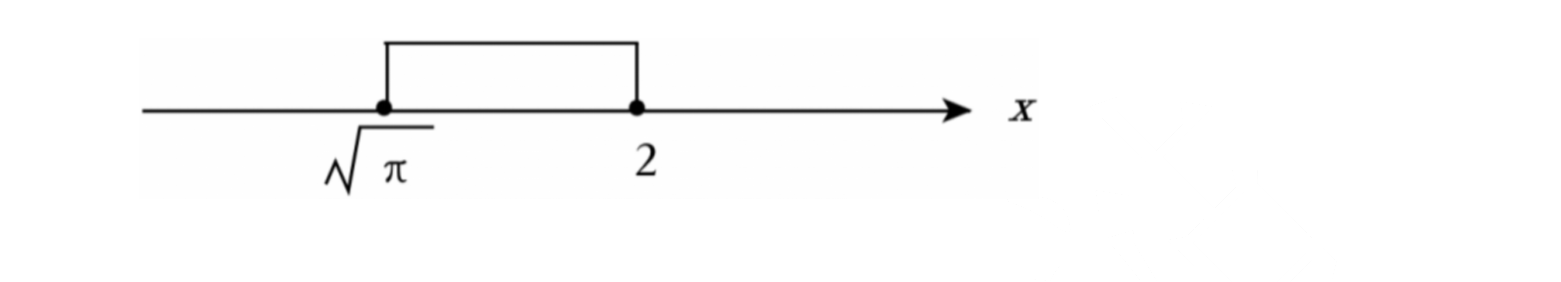
\includegraphics[width=0.72\textwidth]{figures/gao74_q8_numline.png}
\end{center}
\step{所以数形结合得所求集为 $[\sqrt\pi,2]$.}
\solend
\fi

\item 已知集合 $A=\{x\mid(a-1)x^2+3x-3=0,\,x\in\R\}$ 有且仅有一个真子集，则实数 $a=$\blankline[4.4em].

\ifanswer
\solbegin
\step{因为集合 $A=\{x\mid(a-1)x^2+3x-3=0,\,x\in\R\}$ 有且仅有一个真子集，}
\step{所以 $(a-1)x^2+3x-3=0$ 只有一个解，}
\step{所以 $a=1$ 或 $\begin{cases}a\neq1\\ \Delta=3^2-4(a-1)\times(-3)=0\end{cases}$，解得 $a=1$ 或 $a=\dfrac14$.}
\solend
\fi

\item 已知全集 $U=\{(x,y)\mid x,y\in\R\}$，若集合 $A\subseteq U$，且对任意 $(x_1,y_1)\in A$，均存在 $(x_2,y_2)\in A$，使得 $x_1y_2+x_2y_1=0$，则称集合 $A$ 为“对称对点集”. 给出如下集合：

（1）$A=\{(x,y)\mid x,y\in\Z\}$；

（2）$A=\left\{(x,y)\,\middle|\,y=\begin{cases}x+1,&x\geqslant0\\ -x+1,&x<0\end{cases},\ x\in\R,\ x\neq0\right\}$；

（3）$A=\{(x,y)\mid y=x+2,\,x\in\R\}$；

（4）$A=\left\{(x,y)\,\middle|\,y=\dfrac1x,\ x\in\R,\ x\neq0\right\}$.

其中是“对称对点集”的序号为\blankline[4.4em]（写出所有正确的序号）.

\ifanswer
\solbegin
\stepm{(1)}{因为 $0\in\Z$，所以 $(0,0)\in A$.}
\step{对任意 $(x_1,y_1)\in A$，取 $(x_2,y_2)=(0,0)\in A$，}
\step{都有 $x_1\times0+0\times y_1=0$，所以（1）是对称对点集.}
\stepm{(2)}{当 $x_1>0$ 时 $y_1=x_1+1$，取 $x_2=-x_1<0$、$y_2=-x_2+1=x_1+1=y_1$，}
\step{则 $(x_2,y_2)\in A$，且 $x_1y_2+x_2y_1=x_1y_1-x_1y_1=0$；}
\step{当 $x_1<0$ 时同理取 $x_2=-x_1>0$、$y_2=x_2+1=y_1$，}
\step{也有 $(x_2,y_2)\in A$ 且 $x_1y_2+x_2y_1=0$；所以（2）是对称对点集.}
\stepm{(3)}{取 $A$ 中的点 $(-1,1)$. 若存在 $(x_2,y_2)\in A$ 使 $(-1)\cdot y_2+x_2\cdot1=0$，}
\step{则 $y_2=x_2$，但 $A$ 中点的坐标满足 $y=x+2$，两者矛盾，}
\step{所以（3）不是对称对点集.}
\stepm{(4)}{设 $(x_1,y_1)\in A$，则 $x_1\neq0$ 且 $y_1=\dfrac1{x_1}$，}
\step{若存在 $(x_2,y_2)\in A$ 使 $x_1y_2+x_2y_1=0$，}
\step{把 $y_1=\dfrac1{x_1}$、$y_2=\dfrac1{x_2}$（$x_2\neq0$）代入得 $\dfrac{x_1}{x_2}+\dfrac{x_2}{x_1}=0$，即 $x_1^2+x_2^2=0$，}
\step{于是 $x_1=x_2=0$，与 $x_1\neq0$、$x_2\neq0$ 矛盾，所以（4）不是对称对点集.}
\step{故正确的是①②.}
\solend
\fi

\end{enumerate}

\bigsec{二、选择题}

\begin{enumerate}
\setcounter{enumi}{10}

\item “$x>3$”是“$\dfrac{x-1}{x-3}>0$”的\mbox{（\quad）}

\keepwithprev
A. 充分不必要条件\qquad B. 必要不充分条件\qquad C. 充要条件\qquad D. 既不充分也不必要条件

\ifanswer
\solbegin
\step{由 $\dfrac{x-1}{x-3}>0$ 得 $x>3$ 或 $x<1$，故“$x>3$”是“$\dfrac{x-1}{x-3}>0$”的充分不必要条件.}
\step{故选 $A$.}
\solend
\fi

\item 已知 $a,b,c\in\R$，$b>c$，则下列不等式中恒成立的是\mbox{（\quad）}

\keepwithprev
A. $a+b^2>a+c^2$\qquad B. $a^2+b>a^2+c$\qquad C. $ab^2>ac^2$\qquad D. $a^2b>a^2c$

\ifanswer
\solbegin
\step{对于 $A$，取 $b=1,c=-1$，错误；对于 $B$，由不等式的同向可加性得正确；}
\step{对于 $C$，取 $a=1,b=1,c=-2$，错误；对于 $D$，取 $a=0$，错误.}
\step{故选 $B$.}
\solend
\fi

\item 已知关于 $x$ 的不等式 $x^2-2kx+1>0$ 对于一切实数 $x$ 都成立，则实数 $k$ 的取值范围是\mbox{（\quad）}

\keepwithprev
A. $[-1,1]$\qquad B. $(-1,1)$\qquad C. $(-\infty,-1)\cup(1,+\infty)$\qquad D. $\left(-\dfrac12,\dfrac12\right)$

\ifanswer
\solbegin
\step{因为关于 $x$ 的不等式 $x^2-2kx+1>0$ 对于一切实数 $x$ 都成立，}
\step{所以 $\Delta=(-2k)^2-4<0$，即 $4k^2-4<0$，解得 $-1<k<1$，}
\step{所以实数 $k$ 的取值范围是 $(-1,1)$. 故选 $B$.}
\solend
\fi

\item 某种生产设备购买时费用 $100$ 千元，每年的设备管理费 $8$ 千元，这种生产设备的维修费前 $x(x\in\N)$ 年共 $\dfrac{25}{36}x^2+2x$ 千元，问这种生产设备最多使用\mbox{（\quad）}年报废最合算？（即年平均费用最少）

\keepwithprev
A. $13$\qquad B. $10$\qquad C. $15$\qquad D. $12$

\ifanswer
\solbegin
\step{设使用 $x$ 年报废，则总费用 $S(x)=100+8x+\dfrac{25}{36}x^2+2x=\dfrac{25}{36}x^2+10x+100$，}
\step{则年平均费用为 $y=\dfrac{S(x)}x=\dfrac{25x}{36}+\dfrac{100}x+10\geqslant2\sqrt{\dfrac{25x}{36}\cdot\dfrac{100}x}+10=\dfrac{80}3$，}
\step{当且仅当 $\dfrac{25x}{36}=\dfrac{100}x$，即 $x=12$ 时，取等号，}
\step{故当使用 $12$ 年报废，年平均费用最少. 故选 $D$.}
\solend
\fi

\end{enumerate}

\bigsec{三、解答题}

\begin{enumerate}
\setcounter{enumi}{14}

\item （1）设集合 $A=\{x\mid ax-1=0,\,x\in\R\}$，$B=\{x\mid x^2-3x+2=0,\,x\in\R\}$，若 $A\cap B\neq\varnothing$，求实数 $a$ 的取值范围；

（2）已知一元二次方程 $x^2-mx+m+1=0$ 的两个不等实根为 $x_1$、$x_2$，且 $x_1^2+x_2^2=1$，求实数 $m$ 的值.

\ifanswer
\solbegin
\stepm{(1)}{$B=\{x\mid x^2-3x+2=0,\,x\in\R\}=\{1,2\}$，}
\step{①当 $a=0$ 时，方程 $0\cdot x-1=0$ 无解，$A=\varnothing$，$A\cap B=\varnothing$，不符合题意；}
\step{②当 $a\neq0$ 时，$A=\left\{\dfrac1a\right\}$. $A\cap B\neq\varnothing$，}
\step{则 $\dfrac1a\in B$，即 $\dfrac1a=1$ 或 $\dfrac1a=2$，解得 $a=1$ 或 $\dfrac12$；}
\stepm{(2)}{方程 $x^2-mx+m+1=0$ 有两个不等实根，}
\step{则 $\Delta=m^2-4(m+1)>0$，解得 $m>2+2\sqrt2$ 或 $m<2-2\sqrt2$，}
\step{由韦达定理得 $x_1+x_2=m$，$x_1x_2=m+1$，$x_1^2+x_2^2=1$，}
\step{则 $(x_1+x_2)^2-2x_1x_2=m^2-2(m+1)=1$，解得 $m=-1$ 或 $m=3$（舍去），}
\step{综上所述，$m=-1$.}
\solend
\fi

\ansspace

\item 设全集为 $\R$，已知集合 $A=\{x\mid|x-1|\leqslant3,\,x\in\R\}$，

$B=\{x\mid x^2-2mx+(m-3)(m+3)\leqslant0,\,x\in\R\}$.

（1）若 $A\cap B=[0,4]$，求实数 $m$ 的值；

（2）若 $A\cap\overline{B}=A$，求实数 $m$ 的取值范围.

\ifanswer
\solbegin
\stepm{(1)}{$A=\{x\mid|x-1|\leqslant3\}=\{x\mid-2\leqslant x\leqslant4\}$，}
\step{$B=\{x\mid x^2-2mx+(m-3)(m+3)\leqslant0\}=\{x\mid m-3\leqslant x\leqslant m+3\}$，}
\step{若 $A\cap B=[0,4]$，则 $m-3=0$，即 $m=3$；}
\stepm{(2)}{若 $A\cap\overline{B}=A$，则 $A\subseteq\overline{B}$，$\overline{B}=\{x\mid x>m+3\text{ 或 }x<m-3\}$，}
\step{所以 $m+3<-2$ 或 $m-3>4$，解得 $m<-5$ 或 $m>7$，}
\step{实数 $m$ 的取值范围为 $\{m\mid m<-5\text{ 或 }m>7\}$.}
\solend
\fi

\ansspace

\item （1）已知 $a$、$b$ 为正实数，若 $a+b>4$，试用反证法证明：$\dfrac{a}{b+2}$ 和 $\dfrac{b}{a+2}$ 中至少有一个\mbox{大于 $\dfrac12$}；

（2）设 $x$、$y$ 为正实数，$m=\sqrt{2x}+\sqrt{2y}$，$n=\sqrt{x^2+5xy+y^2}$，试比较 $m$、$n$ 的大小，并说明理由.

\ifanswer
\solbegin
\stepm{(1)}{假设 $\dfrac{a}{b+2}\leqslant\dfrac12$ 且 $\dfrac{b}{a+2}\leqslant\dfrac12$，}
\step{又由 $a$、$b$ 为正实数，则有 $2a\leqslant b+2$ 且 $2b\leqslant a+2$，}
\step{两式相加，有 $2a+2b\leqslant a+b+4$，变形得 $a+b\leqslant4$，}
\step{与已知 $a+b>4$ 相矛盾，即假设 $\dfrac{a}{b+2}\leqslant\dfrac12$ 且 $\dfrac{b}{a+2}\leqslant\dfrac12$ 不成立，}
\step{故 $\dfrac{a}{b+2}$ 和 $\dfrac{b}{a+2}$ 中至少有一个\mbox{大于 $\dfrac12$}；}
\stepm{(2)}{$m>n$，理由：$x$、$y$ 为正实数，$m=\sqrt{2x}+\sqrt{2y}$，$n=\sqrt{x^2+5xy+y^2}$，}
\step{则 $m^2=(\sqrt{2x}+\sqrt{2y})^2=2x^2+2y^2+4xy$，$n^2=x^2+y^2+5xy$，}
\step{则有 $m^2-n^2=2x^2+2y^2+4xy-x^2-y^2-5xy=x^2+y^2-xy$}
\step{$=\left(x-\dfrac y2\right)^2+\dfrac{3y^2}4$，}
\step{又 $x$、$y$ 为正实数，则 $m^2-n^2>0$，即 $m^2>n^2$，必有 $m>n$，结论成立.}
\solend
\fi

\ansspace

\item 已知集合 $A=\{a_1,a_2,a_3,\cdots,a_n\}$，$a_i$ 为正整数（$i=1,2,\cdots,n$）.

（1）设 $n=3$，$a_1=1$，$a_2=3$，$a_3=9$，$B=\{a_i+a_j\mid1\leqslant i<j\leqslant3,\,i,j\in\N^*\}$，若互不相同的三个实数 $b_1$、$b_2$、$b_3$，满足 $\{b_i+b_j\mid1\leqslant i<j\leqslant3,\,i,j\in\N^*\}=B$，求有序数组 $(b_1,b_2,b_3)$；

（2）设 $n=4$，$C=\{a_1^2,a_2^2,a_3^2,a_4^2\}$，其中 $a_1<a_2<a_3<a_4$，$A\cap C=\{a_1,a_4\}$，且 $a_1+a_4=10$，$A\cup C$ 中所有元素之和为 $124$，求集合 $A$；

（3）设 $n=2$，有 $7$ 个互不相同的集合 $A$ 分别记为 $A_1$、$A_2$、$A_3$、$\cdots$、$A_7$，且 $A_1\cap A_7=\varnothing$、$A_i\cap A_{i+1}=\varnothing\,(i=1,2,3,\cdots,6)$，记 $D=A_1\cup A_2\cup A_3\cup\cdots\cup A_7$，求 $D$ 中元素个数的最小值.

\ifanswer
\solbegin
\stepm{(1)}{$B=\{a_i+a_j\mid1\leqslant i<j\leqslant3,\,i,j\in\N^*\}=\{1+3,1+9,3+9\}=\{4,10,12\}$，}
\step{由题意，不妨设 $b_1<b_2<b_3$，}
\step{则三个数两两之和为 $\begin{cases}b_1+b_2=4\\ b_1+b_3=10\\ b_2+b_3=12\end{cases}$，解得 $\begin{cases}b_1=1\\ b_2=3\\ b_3=9\end{cases}$，}
\step{所以满足条件的有序数组为 $1$，$3$，$9$ 三个数字的全部排列，}
\step{所以有序数组 $(b_1,b_2,b_3)$ 为 $(1,3,9),(1,9,3),(3,1,9),(3,9,1),(9,1,3),(9,3,1)$；}
\stepm{(2)}{因为 $A\cap C=\{a_1,a_4\}$，所以 $a_1\in C$，$a_4\in C$，}
\step{所以 $a_1$ 是集合 $A$ 中某个正整数的平方，}
\step{又因为 $a_1$ 是最小的正整数，所以只能是 $a_1=1$，此时满足 $1=1^2$.}
\step{又 $a_1+a_4=10$，所以 $a_4=9$，所以 $9$ 也是集合 $A$ 中某个正整数的平方，}
\step{因为 $3^2=9$，所以 $3\in A$，则有 $a_2=3$ 或 $a_3=3$.}
\step{若 $a_3=3$，则 $A=\{1,a_2,3,9\}$，$C=\{1^2,a_2^2,3^2,9^2\}=\{1,a_2^2,9,81\}$，}
\step{因为 $a_1<a_2<a_3<a_4$，且 $a_2$ 为正整数，所以只能是 $a_2=2$，}
\step{故 $A=\{1,2,3,9\}$，$C=\{1,4,9,81\}$，$A\cap C=\{1,9\}$，符合题意，}
\step{则 $A\cup C=\{1,2,3,4,9,81\}$，此时 $1+2+3+4+9+81=100\neq124$，}
\step{故 $a_3=3$ 不符合题意，所以只能 $a_2=3$，}
\step{故 $A=\{1,3,a_3,9\}$，$C=\{1^2,3^2,a_3^2,9^2\}$，此时 $A\cup C=\{1,3,a_3,9,a_3^2,81\}$，}
\step{则有 $1+3+a_3+9+a_3^2+81=124$，}
\step{即 $a_3^2+a_3-30=(a_3+6)(a_3-5)=0$，解得正整数 $a_3=5$，}
\step{此时 $A=\{1,3,5,9\}$，$C=\{1,9,25,81\}$，$A\cup C=\{1,3,5,9,25,81\}$，}
\step{满足 $A\cap C=\{1,9\}$，$A\cup C$ 中所有元素之和为 $1+3+5+9+25+81=124$，}
\step{故 $A=\{1,3,5,9\}$；}
\stepm{(3)}{当 $n=2$ 时，每个集合 $A_i(i=1,2,\cdots,7)$ 均为含有 $2$ 个元素的二元集合，}
\step{设 $D$ 中元素个数为 $m$，}
\step{若 $m\leqslant4$，从 $m$ 个元素中最多能得到 $\dfrac{4\times3}2=6$ 个不同二元集合，不足 $7$ 个，}
\step{故 $m\leqslant4$ 不可能.}
\step{若 $m=5$，则有 $\dfrac{5\times4}2=10$ 个不同二元集合，数量超过 $7$ 个，符合要求.}
\step{因为 $A_i\cap A_{i+1}=\varnothing(i=1,2,3,\cdots,6)$，$A_1\cap A_7=\varnothing$，}
\step{即要求 $7$ 个互不相同的二元集合排成环，}
\step{且相邻（含首尾）集合交集为空集.}
\needvspace{12\baselineskip}
\step{假设 $m=5$，不妨设 $A_1(1,2)$、$A_2(3,4)$、$A_3(1,5)$，则：}
\begin{center}
\renewcommand{\arraystretch}{1.9}
\begin{tabular}{|c|c|c|c|c|}
\hline
$A_4(2,3)$ & $A_5(1,4)$ & $A_6(2,5)$ & $A_7(1,3)$ & 与 $A_1$ 矛盾\\
\hline
 &  & $A_6(3,5)$ & $A_7(2,4)$ & 与 $A_1$ 矛盾\\
\hline
 & $A_5(4,5)$ & $A_6(1,3)$ & $A_7(2,5)$ 或 $A_7(2,4)$ & 与 $A_1$ 矛盾\\
\hline
$A_4(2,4)$ & $A_5(1,3)$ & $A_6(2,5)$ & $A_7(1,4)$ & 与 $A_1$ 矛盾\\
\hline
 &  & $A_6(4,5)$ & $A_7(2,3)$ & 与 $A_1$ 矛盾\\
\hline
 & $A_5(3,5)$ & $A_6(1,4)$ & $A_7(2,3)$ 或 $A_7(2,5)$ & 与 $A_1$ 矛盾\\
\hline
\end{tabular}
\end{center}
\step{故 $m=5$ 不可能.}
\step{综上，$m\geqslant6$，取 $D=\{1,2,3,4,5,6\}$，}
\step{令 $A_1=\{1,2\},A_2=\{3,4\},A_3=\{1,5\},A_4=\{2,4\},A_5=\{3,6\},A_6=\{1,4\}$，}
\step{$A_7=\{5,6\}$，此时 $A_1$、$A_2$、$\cdots$、$A_7$ 是 $7$ 个互不相同的二元集合，}
\step{且 $A_1\cap A_2=\varnothing$，$A_2\cap A_3=\varnothing$，$A_3\cap A_4=\varnothing$，$A_4\cap A_5=\varnothing$，}
\step{$A_5\cap A_6=\varnothing$，$A_6\cap A_7=\varnothing$，$A_7\cap A_1=\varnothing$，满足全部条件，}
\step{故 $D$ 中元素个数的最小值为 $6$.}
\solend
\fi

\ansspace*[7]

\end{enumerate}

\end{document}
"
% 紧凑版：xelatex "\def\iscompact{1}% 高一74_宜川中学_10月月考.tex
%   —— 高一上数学“2026-2027 年宜川中学高一上 10 月月考”（讲评版）
% 试卷版：xelatex 高一74_宜川中学_10月月考.tex
% 答案版：xelatex "\def\isanswer{1}% 高一74_宜川中学_10月月考.tex
%   —— 高一上数学“2026-2027 年宜川中学高一上 10 月月考”（讲评版）
% 试卷版：xelatex 高一74_宜川中学_10月月考.tex
% 答案版：xelatex "\def\isanswer{1}\input{高一74_宜川中学_10月月考.tex}"
% 紧凑版：xelatex "\def\iscompact{1}\input{高一74_宜川中学_10月月考.tex}"
%
% 原始材料：微信公众号“魔都数学加油站”文章，连载“27学年高一74”；
% 原文标题“27学年高一74——2026-2027年上海市宜川中学高一上10月月考”；
% 原文链接：https://mp.weixin.qq.com/s/ymsl2bmkBRY6ZPDiUFCDTA。
% 页面标注发布时间 2026-10-22 21:45（上海）。
% 正文为 9 张 PNG 页（`原图/高一74_宜川中学_10月月考/01..09.png`）：
% 第 1、2、3 页为 4762×6735，其余 6 页为 2560×3620，均按页序读取。
% 9 页全为试卷正文页（卷首标题在第 1 页页顶，卷末第 18 题 (3) 解析止于第 9 页），
% 无封面页、目录页、二维码或宣传页。粉色斜排“魔都数学加油站”为卷面水印，未录入。
%
% 卷首标题：照卷面印作“2026-2027 年宜川中学高一上 10 月月考”（黑体加粗一行）。
% 原卷年份区间用半角连字符，本稿按全稿惯例排 en dash；原卷无副标题。
%
% 篇幅与题号：原卷自第 3 题起编号（第 1、2 题不在本卷内）。填空题 3—10（8 题）、
% 选择题 11—14（4 题）、解答题 15—18（4 题），共 16 题。本稿沿用原节与原题号，
% 只改排为全稿统一的大节样式。
%
% 讲评版：原卷第 3 题只印【答案】（“{(1,1)}”），本稿只给 \ans{}；其余 15 题均印
% 【解析】，用 \solbegin…\solend。四道选择题的作答括号原卷即留空，答案写在解析末句
% “故选 A／B／B／D”，照录在解析内，不另提 \ans{}。
%
% 副标题：原卷未印副标题。本稿按“知识模块”口径标作“集合与常用逻辑用语、不等式”：
% 16 题中集合与常用逻辑用语 7 题（第 3、9、10、15、16、18 题及第 17 题的反证法），
% 不等式 9 题（第 4—8、11—14、17 题），两类均确有分量，故并标。口径同 高一63、高一68—73。
%
% 与原卷的排版差异：
%   ① 原卷每题下直接印【答案】/【解析】，本稿按全稿惯例将答案与解析置于答案版；
%   ② 原卷未印副标题，本稿按“知识模块”口径补出；
%   ③ 原卷填空横线约四个字宽，本稿按全稿惯例统一排 \blankline[4.4em]；
%   ④ 原卷数集记号排斜体 $R$、$Z$、$N$（第 8、9、10、14—18 题），本稿按全稿惯例
%      改用 $\R$、$\Z$、$\N$（同 高一68—73）；第 18 题的正整数集合作 $\N^*$，照录；
%   ⑤ 原卷句末标点多为西文句点，均逐处照录；
%   ⑥ 第 15—18 题的子问原卷印作“（1）…（2）…”，本稿按 高一69—73 成例用行内
%      “（1）（2）（3）”段，解析中的子问标号用 \stepm{(1)}{…}；
%   ⑦ 每道解答题原卷未留作答空白，本稿按全稿惯例加 \ansspace（末题用 \ansspace*）；
%   ⑧ 选择题的作答括号原卷排半角“(    )”，本稿按全稿惯例排 \mbox{（\quad）}；
%      选项行排照原卷——第 11、13 题一行四条，第 12、14 题一行四条；
%   ⑨ 第 9、14、18 题解析中的不等式组／方程组，原卷均排作“{”连接的多行式，
%      本稿按全稿惯例排 cases；
%   ⑩ 第 8 题解析有一幅数轴图：原卷印在【解析】第 2 行之后，题干无“如图”二字。
%      本稿按原卷截图裁取（`figures/gao74_q8_numline.png`，由第 2 页原图裁出、
%      去除粉色水印后转灰度，未放大），放在答案版解析第 2 条之后；
%   ⑪ 第 18 题 (3) 解析中有一张 5 列 6 行的枚举表（原卷无表头、左侧两列留空以表示
%      沿用上格的 $A_4$／$A_5$），本稿照原卷排成同样的空格表，未加表头、未合并单元格。
%
% 原卷笔误/存疑（均照录未改，正文对应处另有 % 注）：
%   ① 第 14 题题干“维修费前 $x(x\in N)$ 年共 $\dfrac{25}{36}x^2+2x$ 千元”中的
%      $N$ 原卷排斜体，按全稿惯例改 $\N$，含义不变；
%   ② 第 18 题 (3) 的枚举表第 1—3 行与第 4—6 行分属“$A_5(1,4)$”“$A_5(1,3)$”两种
%      情形，原卷只在首行重复写 $A_4$、$A_5$，其余留空；本稿照录留空，未补字。
%
% 行数核对：逐题数 \step/\stepm 条数与原卷【解析】印刷行数，15 题逐一相符，
% 合计 104 条 / 104 行（Q4：1；Q5：2；Q6：3；Q7：3；Q8：3；Q9：3；Q10：15；
% Q11：2；Q12：3；Q13：3；Q14：4；Q15：9；Q16：6；Q17：10；Q18：37）。
% 另第 3 题只印【答案】，提 \ans{}，不计入 \step 账。
%
% 插图：第 8 题解析的数轴图，见上⑩；全卷题干无其他配图。
%
\documentclass[a4paper,11pt]{article}
\usepackage{common}

\begin{document}

\examtitlest[3]{2026--2027 年宜川中学高一上 10 月月考}{集合与常用逻辑用语、不等式}

\bigsec{一、填空题}

\begin{enumerate}
\setcounter{enumi}{2}

\item 已知集合 $A=\{(x,y)\mid y=x\}$，集合 $B=\{(x,y)\mid y=2-x\}$，则 $A\cap B=$\blankline[4.4em].

\ifanswer
\ans{$\{(1,1)\}$}
\fi

\item 已知 $a=\log_3 2$，$b=\log_3 8$，则 $3^{2a-b}=$\blankline[4.4em].

\ifanswer
\solbegin
\step{由 $a=\log_3 2$，$b=\log_3 8$，得 $3^a=2$，$3^b=8$，则 $3^{2a-b}=\dfrac{(3^a)^2}{3^b}=\dfrac48=\dfrac12$.}
\solend
\fi

\item 已知等式 $2x^2+3x+5=a(2x+1)(x+1)+c$ 恒成立，则实数 $c=$\blankline[4.4em].

\ifanswer
\solbegin
\step{$2x^2+3x+5=a(2x+1)(x+1)+c=2ax^2+3ax+a+c$，}
\step{则 $\begin{cases}2a=2\\ 3a=3\\ a+c=5\end{cases}$，解得 $c=4$.}
\solend
\fi

\item 已知 $x>0$，$y>0$，且 $\dfrac9x+\dfrac1y=1$，则 $x\cdot y$ 的最小值是\blankline[4.4em].

\ifanswer
\solbegin
\step{$x>0$，$y>0$，且 $1=\dfrac9x+\dfrac1y\geqslant2\sqrt{\dfrac9{xy}}$，}
\step{当且仅当 $x=9y$，即 $y=2$，$x=18$ 时取等号，所以 $xy\geqslant36$，}
\step{则 $x\cdot y$ 的最小值为 $36$.}
\solend
\fi

\item 已知关于 $x$ 的不等式 $x^2+bx+c>0$（$b$、$c$ 为实数）的解集为 $(-\infty,-2)\cup(3,+\infty)$，则不等式 $cx^2-bx+1\leqslant0$ 的解集为\blankline[4.4em].

\ifanswer
\solbegin
\step{由已知得 $-2$、$3$ 为方程 $x^2+bx+c=0$ 的根，所以 $-2+3=-b$，$-2\times3=c$，}
\step{即 $b=-1$，$c=-6$，所以不等式 $cx^2-bx+1\leqslant0$ 可变形为 $-6x^2+x+1\leqslant0$，}
\step{即 $6x^2-x-1\geqslant0$，解得 $x\leqslant-\dfrac13$ 或 $x\geqslant\dfrac12$，所以解集为 $\left(-\infty,-\dfrac13\right]\cup\left[\dfrac12,+\infty\right)$.}
\solend
\fi

\item 设 $x\in\R$，则方程 $|x-2|+|\sqrt\pi-x|=2-\sqrt\pi$ 的解集为\blankline[4.4em].

\ifanswer
\solbegin
\step{因为方程 $|x-2|+|\sqrt\pi-x|=2-\sqrt\pi$ 可化为 $|x-2|+|x-\sqrt\pi|=2-\sqrt\pi$，}
\needvspace{8\baselineskip}
\step{其表示数轴上实数 $x$ 到 $\sqrt\pi$ 与 $2$ 的距离之和等于 $2-\sqrt\pi$，如图：}
\begin{center}
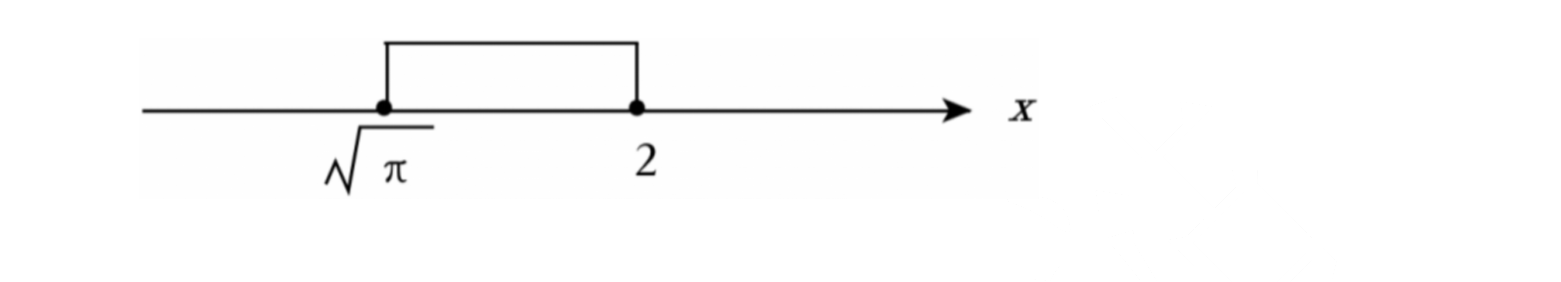
\includegraphics[width=0.72\textwidth]{figures/gao74_q8_numline.png}
\end{center}
\step{所以数形结合得所求集为 $[\sqrt\pi,2]$.}
\solend
\fi

\item 已知集合 $A=\{x\mid(a-1)x^2+3x-3=0,\,x\in\R\}$ 有且仅有一个真子集，则实数 $a=$\blankline[4.4em].

\ifanswer
\solbegin
\step{因为集合 $A=\{x\mid(a-1)x^2+3x-3=0,\,x\in\R\}$ 有且仅有一个真子集，}
\step{所以 $(a-1)x^2+3x-3=0$ 只有一个解，}
\step{所以 $a=1$ 或 $\begin{cases}a\neq1\\ \Delta=3^2-4(a-1)\times(-3)=0\end{cases}$，解得 $a=1$ 或 $a=\dfrac14$.}
\solend
\fi

\item 已知全集 $U=\{(x,y)\mid x,y\in\R\}$，若集合 $A\subseteq U$，且对任意 $(x_1,y_1)\in A$，均存在 $(x_2,y_2)\in A$，使得 $x_1y_2+x_2y_1=0$，则称集合 $A$ 为“对称对点集”. 给出如下集合：

（1）$A=\{(x,y)\mid x,y\in\Z\}$；

（2）$A=\left\{(x,y)\,\middle|\,y=\begin{cases}x+1,&x\geqslant0\\ -x+1,&x<0\end{cases},\ x\in\R,\ x\neq0\right\}$；

（3）$A=\{(x,y)\mid y=x+2,\,x\in\R\}$；

（4）$A=\left\{(x,y)\,\middle|\,y=\dfrac1x,\ x\in\R,\ x\neq0\right\}$.

其中是“对称对点集”的序号为\blankline[4.4em]（写出所有正确的序号）.

\ifanswer
\solbegin
\stepm{(1)}{因为 $0\in\Z$，所以 $(0,0)\in A$.}
\step{对任意 $(x_1,y_1)\in A$，取 $(x_2,y_2)=(0,0)\in A$，}
\step{都有 $x_1\times0+0\times y_1=0$，所以（1）是对称对点集.}
\stepm{(2)}{当 $x_1>0$ 时 $y_1=x_1+1$，取 $x_2=-x_1<0$、$y_2=-x_2+1=x_1+1=y_1$，}
\step{则 $(x_2,y_2)\in A$，且 $x_1y_2+x_2y_1=x_1y_1-x_1y_1=0$；}
\step{当 $x_1<0$ 时同理取 $x_2=-x_1>0$、$y_2=x_2+1=y_1$，}
\step{也有 $(x_2,y_2)\in A$ 且 $x_1y_2+x_2y_1=0$；所以（2）是对称对点集.}
\stepm{(3)}{取 $A$ 中的点 $(-1,1)$. 若存在 $(x_2,y_2)\in A$ 使 $(-1)\cdot y_2+x_2\cdot1=0$，}
\step{则 $y_2=x_2$，但 $A$ 中点的坐标满足 $y=x+2$，两者矛盾，}
\step{所以（3）不是对称对点集.}
\stepm{(4)}{设 $(x_1,y_1)\in A$，则 $x_1\neq0$ 且 $y_1=\dfrac1{x_1}$，}
\step{若存在 $(x_2,y_2)\in A$ 使 $x_1y_2+x_2y_1=0$，}
\step{把 $y_1=\dfrac1{x_1}$、$y_2=\dfrac1{x_2}$（$x_2\neq0$）代入得 $\dfrac{x_1}{x_2}+\dfrac{x_2}{x_1}=0$，即 $x_1^2+x_2^2=0$，}
\step{于是 $x_1=x_2=0$，与 $x_1\neq0$、$x_2\neq0$ 矛盾，所以（4）不是对称对点集.}
\step{故正确的是①②.}
\solend
\fi

\end{enumerate}

\bigsec{二、选择题}

\begin{enumerate}
\setcounter{enumi}{10}

\item “$x>3$”是“$\dfrac{x-1}{x-3}>0$”的\mbox{（\quad）}

\keepwithprev
A. 充分不必要条件\qquad B. 必要不充分条件\qquad C. 充要条件\qquad D. 既不充分也不必要条件

\ifanswer
\solbegin
\step{由 $\dfrac{x-1}{x-3}>0$ 得 $x>3$ 或 $x<1$，故“$x>3$”是“$\dfrac{x-1}{x-3}>0$”的充分不必要条件.}
\step{故选 $A$.}
\solend
\fi

\item 已知 $a,b,c\in\R$，$b>c$，则下列不等式中恒成立的是\mbox{（\quad）}

\keepwithprev
A. $a+b^2>a+c^2$\qquad B. $a^2+b>a^2+c$\qquad C. $ab^2>ac^2$\qquad D. $a^2b>a^2c$

\ifanswer
\solbegin
\step{对于 $A$，取 $b=1,c=-1$，错误；对于 $B$，由不等式的同向可加性得正确；}
\step{对于 $C$，取 $a=1,b=1,c=-2$，错误；对于 $D$，取 $a=0$，错误.}
\step{故选 $B$.}
\solend
\fi

\item 已知关于 $x$ 的不等式 $x^2-2kx+1>0$ 对于一切实数 $x$ 都成立，则实数 $k$ 的取值范围是\mbox{（\quad）}

\keepwithprev
A. $[-1,1]$\qquad B. $(-1,1)$\qquad C. $(-\infty,-1)\cup(1,+\infty)$\qquad D. $\left(-\dfrac12,\dfrac12\right)$

\ifanswer
\solbegin
\step{因为关于 $x$ 的不等式 $x^2-2kx+1>0$ 对于一切实数 $x$ 都成立，}
\step{所以 $\Delta=(-2k)^2-4<0$，即 $4k^2-4<0$，解得 $-1<k<1$，}
\step{所以实数 $k$ 的取值范围是 $(-1,1)$. 故选 $B$.}
\solend
\fi

\item 某种生产设备购买时费用 $100$ 千元，每年的设备管理费 $8$ 千元，这种生产设备的维修费前 $x(x\in\N)$ 年共 $\dfrac{25}{36}x^2+2x$ 千元，问这种生产设备最多使用\mbox{（\quad）}年报废最合算？（即年平均费用最少）

\keepwithprev
A. $13$\qquad B. $10$\qquad C. $15$\qquad D. $12$

\ifanswer
\solbegin
\step{设使用 $x$ 年报废，则总费用 $S(x)=100+8x+\dfrac{25}{36}x^2+2x=\dfrac{25}{36}x^2+10x+100$，}
\step{则年平均费用为 $y=\dfrac{S(x)}x=\dfrac{25x}{36}+\dfrac{100}x+10\geqslant2\sqrt{\dfrac{25x}{36}\cdot\dfrac{100}x}+10=\dfrac{80}3$，}
\step{当且仅当 $\dfrac{25x}{36}=\dfrac{100}x$，即 $x=12$ 时，取等号，}
\step{故当使用 $12$ 年报废，年平均费用最少. 故选 $D$.}
\solend
\fi

\end{enumerate}

\bigsec{三、解答题}

\begin{enumerate}
\setcounter{enumi}{14}

\item （1）设集合 $A=\{x\mid ax-1=0,\,x\in\R\}$，$B=\{x\mid x^2-3x+2=0,\,x\in\R\}$，若 $A\cap B\neq\varnothing$，求实数 $a$ 的取值范围；

（2）已知一元二次方程 $x^2-mx+m+1=0$ 的两个不等实根为 $x_1$、$x_2$，且 $x_1^2+x_2^2=1$，求实数 $m$ 的值.

\ifanswer
\solbegin
\stepm{(1)}{$B=\{x\mid x^2-3x+2=0,\,x\in\R\}=\{1,2\}$，}
\step{①当 $a=0$ 时，方程 $0\cdot x-1=0$ 无解，$A=\varnothing$，$A\cap B=\varnothing$，不符合题意；}
\step{②当 $a\neq0$ 时，$A=\left\{\dfrac1a\right\}$. $A\cap B\neq\varnothing$，}
\step{则 $\dfrac1a\in B$，即 $\dfrac1a=1$ 或 $\dfrac1a=2$，解得 $a=1$ 或 $\dfrac12$；}
\stepm{(2)}{方程 $x^2-mx+m+1=0$ 有两个不等实根，}
\step{则 $\Delta=m^2-4(m+1)>0$，解得 $m>2+2\sqrt2$ 或 $m<2-2\sqrt2$，}
\step{由韦达定理得 $x_1+x_2=m$，$x_1x_2=m+1$，$x_1^2+x_2^2=1$，}
\step{则 $(x_1+x_2)^2-2x_1x_2=m^2-2(m+1)=1$，解得 $m=-1$ 或 $m=3$（舍去），}
\step{综上所述，$m=-1$.}
\solend
\fi

\ansspace

\item 设全集为 $\R$，已知集合 $A=\{x\mid|x-1|\leqslant3,\,x\in\R\}$，

$B=\{x\mid x^2-2mx+(m-3)(m+3)\leqslant0,\,x\in\R\}$.

（1）若 $A\cap B=[0,4]$，求实数 $m$ 的值；

（2）若 $A\cap\overline{B}=A$，求实数 $m$ 的取值范围.

\ifanswer
\solbegin
\stepm{(1)}{$A=\{x\mid|x-1|\leqslant3\}=\{x\mid-2\leqslant x\leqslant4\}$，}
\step{$B=\{x\mid x^2-2mx+(m-3)(m+3)\leqslant0\}=\{x\mid m-3\leqslant x\leqslant m+3\}$，}
\step{若 $A\cap B=[0,4]$，则 $m-3=0$，即 $m=3$；}
\stepm{(2)}{若 $A\cap\overline{B}=A$，则 $A\subseteq\overline{B}$，$\overline{B}=\{x\mid x>m+3\text{ 或 }x<m-3\}$，}
\step{所以 $m+3<-2$ 或 $m-3>4$，解得 $m<-5$ 或 $m>7$，}
\step{实数 $m$ 的取值范围为 $\{m\mid m<-5\text{ 或 }m>7\}$.}
\solend
\fi

\ansspace

\item （1）已知 $a$、$b$ 为正实数，若 $a+b>4$，试用反证法证明：$\dfrac{a}{b+2}$ 和 $\dfrac{b}{a+2}$ 中至少有一个\mbox{大于 $\dfrac12$}；

（2）设 $x$、$y$ 为正实数，$m=\sqrt{2x}+\sqrt{2y}$，$n=\sqrt{x^2+5xy+y^2}$，试比较 $m$、$n$ 的大小，并说明理由.

\ifanswer
\solbegin
\stepm{(1)}{假设 $\dfrac{a}{b+2}\leqslant\dfrac12$ 且 $\dfrac{b}{a+2}\leqslant\dfrac12$，}
\step{又由 $a$、$b$ 为正实数，则有 $2a\leqslant b+2$ 且 $2b\leqslant a+2$，}
\step{两式相加，有 $2a+2b\leqslant a+b+4$，变形得 $a+b\leqslant4$，}
\step{与已知 $a+b>4$ 相矛盾，即假设 $\dfrac{a}{b+2}\leqslant\dfrac12$ 且 $\dfrac{b}{a+2}\leqslant\dfrac12$ 不成立，}
\step{故 $\dfrac{a}{b+2}$ 和 $\dfrac{b}{a+2}$ 中至少有一个\mbox{大于 $\dfrac12$}；}
\stepm{(2)}{$m>n$，理由：$x$、$y$ 为正实数，$m=\sqrt{2x}+\sqrt{2y}$，$n=\sqrt{x^2+5xy+y^2}$，}
\step{则 $m^2=(\sqrt{2x}+\sqrt{2y})^2=2x^2+2y^2+4xy$，$n^2=x^2+y^2+5xy$，}
\step{则有 $m^2-n^2=2x^2+2y^2+4xy-x^2-y^2-5xy=x^2+y^2-xy$}
\step{$=\left(x-\dfrac y2\right)^2+\dfrac{3y^2}4$，}
\step{又 $x$、$y$ 为正实数，则 $m^2-n^2>0$，即 $m^2>n^2$，必有 $m>n$，结论成立.}
\solend
\fi

\ansspace

\item 已知集合 $A=\{a_1,a_2,a_3,\cdots,a_n\}$，$a_i$ 为正整数（$i=1,2,\cdots,n$）.

（1）设 $n=3$，$a_1=1$，$a_2=3$，$a_3=9$，$B=\{a_i+a_j\mid1\leqslant i<j\leqslant3,\,i,j\in\N^*\}$，若互不相同的三个实数 $b_1$、$b_2$、$b_3$，满足 $\{b_i+b_j\mid1\leqslant i<j\leqslant3,\,i,j\in\N^*\}=B$，求有序数组 $(b_1,b_2,b_3)$；

（2）设 $n=4$，$C=\{a_1^2,a_2^2,a_3^2,a_4^2\}$，其中 $a_1<a_2<a_3<a_4$，$A\cap C=\{a_1,a_4\}$，且 $a_1+a_4=10$，$A\cup C$ 中所有元素之和为 $124$，求集合 $A$；

（3）设 $n=2$，有 $7$ 个互不相同的集合 $A$ 分别记为 $A_1$、$A_2$、$A_3$、$\cdots$、$A_7$，且 $A_1\cap A_7=\varnothing$、$A_i\cap A_{i+1}=\varnothing\,(i=1,2,3,\cdots,6)$，记 $D=A_1\cup A_2\cup A_3\cup\cdots\cup A_7$，求 $D$ 中元素个数的最小值.

\ifanswer
\solbegin
\stepm{(1)}{$B=\{a_i+a_j\mid1\leqslant i<j\leqslant3,\,i,j\in\N^*\}=\{1+3,1+9,3+9\}=\{4,10,12\}$，}
\step{由题意，不妨设 $b_1<b_2<b_3$，}
\step{则三个数两两之和为 $\begin{cases}b_1+b_2=4\\ b_1+b_3=10\\ b_2+b_3=12\end{cases}$，解得 $\begin{cases}b_1=1\\ b_2=3\\ b_3=9\end{cases}$，}
\step{所以满足条件的有序数组为 $1$，$3$，$9$ 三个数字的全部排列，}
\step{所以有序数组 $(b_1,b_2,b_3)$ 为 $(1,3,9),(1,9,3),(3,1,9),(3,9,1),(9,1,3),(9,3,1)$；}
\stepm{(2)}{因为 $A\cap C=\{a_1,a_4\}$，所以 $a_1\in C$，$a_4\in C$，}
\step{所以 $a_1$ 是集合 $A$ 中某个正整数的平方，}
\step{又因为 $a_1$ 是最小的正整数，所以只能是 $a_1=1$，此时满足 $1=1^2$.}
\step{又 $a_1+a_4=10$，所以 $a_4=9$，所以 $9$ 也是集合 $A$ 中某个正整数的平方，}
\step{因为 $3^2=9$，所以 $3\in A$，则有 $a_2=3$ 或 $a_3=3$.}
\step{若 $a_3=3$，则 $A=\{1,a_2,3,9\}$，$C=\{1^2,a_2^2,3^2,9^2\}=\{1,a_2^2,9,81\}$，}
\step{因为 $a_1<a_2<a_3<a_4$，且 $a_2$ 为正整数，所以只能是 $a_2=2$，}
\step{故 $A=\{1,2,3,9\}$，$C=\{1,4,9,81\}$，$A\cap C=\{1,9\}$，符合题意，}
\step{则 $A\cup C=\{1,2,3,4,9,81\}$，此时 $1+2+3+4+9+81=100\neq124$，}
\step{故 $a_3=3$ 不符合题意，所以只能 $a_2=3$，}
\step{故 $A=\{1,3,a_3,9\}$，$C=\{1^2,3^2,a_3^2,9^2\}$，此时 $A\cup C=\{1,3,a_3,9,a_3^2,81\}$，}
\step{则有 $1+3+a_3+9+a_3^2+81=124$，}
\step{即 $a_3^2+a_3-30=(a_3+6)(a_3-5)=0$，解得正整数 $a_3=5$，}
\step{此时 $A=\{1,3,5,9\}$，$C=\{1,9,25,81\}$，$A\cup C=\{1,3,5,9,25,81\}$，}
\step{满足 $A\cap C=\{1,9\}$，$A\cup C$ 中所有元素之和为 $1+3+5+9+25+81=124$，}
\step{故 $A=\{1,3,5,9\}$；}
\stepm{(3)}{当 $n=2$ 时，每个集合 $A_i(i=1,2,\cdots,7)$ 均为含有 $2$ 个元素的二元集合，}
\step{设 $D$ 中元素个数为 $m$，}
\step{若 $m\leqslant4$，从 $m$ 个元素中最多能得到 $\dfrac{4\times3}2=6$ 个不同二元集合，不足 $7$ 个，}
\step{故 $m\leqslant4$ 不可能.}
\step{若 $m=5$，则有 $\dfrac{5\times4}2=10$ 个不同二元集合，数量超过 $7$ 个，符合要求.}
\step{因为 $A_i\cap A_{i+1}=\varnothing(i=1,2,3,\cdots,6)$，$A_1\cap A_7=\varnothing$，}
\step{即要求 $7$ 个互不相同的二元集合排成环，}
\step{且相邻（含首尾）集合交集为空集.}
\needvspace{12\baselineskip}
\step{假设 $m=5$，不妨设 $A_1(1,2)$、$A_2(3,4)$、$A_3(1,5)$，则：}
\begin{center}
\renewcommand{\arraystretch}{1.9}
\begin{tabular}{|c|c|c|c|c|}
\hline
$A_4(2,3)$ & $A_5(1,4)$ & $A_6(2,5)$ & $A_7(1,3)$ & 与 $A_1$ 矛盾\\
\hline
 &  & $A_6(3,5)$ & $A_7(2,4)$ & 与 $A_1$ 矛盾\\
\hline
 & $A_5(4,5)$ & $A_6(1,3)$ & $A_7(2,5)$ 或 $A_7(2,4)$ & 与 $A_1$ 矛盾\\
\hline
$A_4(2,4)$ & $A_5(1,3)$ & $A_6(2,5)$ & $A_7(1,4)$ & 与 $A_1$ 矛盾\\
\hline
 &  & $A_6(4,5)$ & $A_7(2,3)$ & 与 $A_1$ 矛盾\\
\hline
 & $A_5(3,5)$ & $A_6(1,4)$ & $A_7(2,3)$ 或 $A_7(2,5)$ & 与 $A_1$ 矛盾\\
\hline
\end{tabular}
\end{center}
\step{故 $m=5$ 不可能.}
\step{综上，$m\geqslant6$，取 $D=\{1,2,3,4,5,6\}$，}
\step{令 $A_1=\{1,2\},A_2=\{3,4\},A_3=\{1,5\},A_4=\{2,4\},A_5=\{3,6\},A_6=\{1,4\}$，}
\step{$A_7=\{5,6\}$，此时 $A_1$、$A_2$、$\cdots$、$A_7$ 是 $7$ 个互不相同的二元集合，}
\step{且 $A_1\cap A_2=\varnothing$，$A_2\cap A_3=\varnothing$，$A_3\cap A_4=\varnothing$，$A_4\cap A_5=\varnothing$，}
\step{$A_5\cap A_6=\varnothing$，$A_6\cap A_7=\varnothing$，$A_7\cap A_1=\varnothing$，满足全部条件，}
\step{故 $D$ 中元素个数的最小值为 $6$.}
\solend
\fi

\ansspace*[7]

\end{enumerate}

\end{document}
"
% 紧凑版：xelatex "\def\iscompact{1}% 高一74_宜川中学_10月月考.tex
%   —— 高一上数学“2026-2027 年宜川中学高一上 10 月月考”（讲评版）
% 试卷版：xelatex 高一74_宜川中学_10月月考.tex
% 答案版：xelatex "\def\isanswer{1}\input{高一74_宜川中学_10月月考.tex}"
% 紧凑版：xelatex "\def\iscompact{1}\input{高一74_宜川中学_10月月考.tex}"
%
% 原始材料：微信公众号“魔都数学加油站”文章，连载“27学年高一74”；
% 原文标题“27学年高一74——2026-2027年上海市宜川中学高一上10月月考”；
% 原文链接：https://mp.weixin.qq.com/s/ymsl2bmkBRY6ZPDiUFCDTA。
% 页面标注发布时间 2026-10-22 21:45（上海）。
% 正文为 9 张 PNG 页（`原图/高一74_宜川中学_10月月考/01..09.png`）：
% 第 1、2、3 页为 4762×6735，其余 6 页为 2560×3620，均按页序读取。
% 9 页全为试卷正文页（卷首标题在第 1 页页顶，卷末第 18 题 (3) 解析止于第 9 页），
% 无封面页、目录页、二维码或宣传页。粉色斜排“魔都数学加油站”为卷面水印，未录入。
%
% 卷首标题：照卷面印作“2026-2027 年宜川中学高一上 10 月月考”（黑体加粗一行）。
% 原卷年份区间用半角连字符，本稿按全稿惯例排 en dash；原卷无副标题。
%
% 篇幅与题号：原卷自第 3 题起编号（第 1、2 题不在本卷内）。填空题 3—10（8 题）、
% 选择题 11—14（4 题）、解答题 15—18（4 题），共 16 题。本稿沿用原节与原题号，
% 只改排为全稿统一的大节样式。
%
% 讲评版：原卷第 3 题只印【答案】（“{(1,1)}”），本稿只给 \ans{}；其余 15 题均印
% 【解析】，用 \solbegin…\solend。四道选择题的作答括号原卷即留空，答案写在解析末句
% “故选 A／B／B／D”，照录在解析内，不另提 \ans{}。
%
% 副标题：原卷未印副标题。本稿按“知识模块”口径标作“集合与常用逻辑用语、不等式”：
% 16 题中集合与常用逻辑用语 7 题（第 3、9、10、15、16、18 题及第 17 题的反证法），
% 不等式 9 题（第 4—8、11—14、17 题），两类均确有分量，故并标。口径同 高一63、高一68—73。
%
% 与原卷的排版差异：
%   ① 原卷每题下直接印【答案】/【解析】，本稿按全稿惯例将答案与解析置于答案版；
%   ② 原卷未印副标题，本稿按“知识模块”口径补出；
%   ③ 原卷填空横线约四个字宽，本稿按全稿惯例统一排 \blankline[4.4em]；
%   ④ 原卷数集记号排斜体 $R$、$Z$、$N$（第 8、9、10、14—18 题），本稿按全稿惯例
%      改用 $\R$、$\Z$、$\N$（同 高一68—73）；第 18 题的正整数集合作 $\N^*$，照录；
%   ⑤ 原卷句末标点多为西文句点，均逐处照录；
%   ⑥ 第 15—18 题的子问原卷印作“（1）…（2）…”，本稿按 高一69—73 成例用行内
%      “（1）（2）（3）”段，解析中的子问标号用 \stepm{(1)}{…}；
%   ⑦ 每道解答题原卷未留作答空白，本稿按全稿惯例加 \ansspace（末题用 \ansspace*）；
%   ⑧ 选择题的作答括号原卷排半角“(    )”，本稿按全稿惯例排 \mbox{（\quad）}；
%      选项行排照原卷——第 11、13 题一行四条，第 12、14 题一行四条；
%   ⑨ 第 9、14、18 题解析中的不等式组／方程组，原卷均排作“{”连接的多行式，
%      本稿按全稿惯例排 cases；
%   ⑩ 第 8 题解析有一幅数轴图：原卷印在【解析】第 2 行之后，题干无“如图”二字。
%      本稿按原卷截图裁取（`figures/gao74_q8_numline.png`，由第 2 页原图裁出、
%      去除粉色水印后转灰度，未放大），放在答案版解析第 2 条之后；
%   ⑪ 第 18 题 (3) 解析中有一张 5 列 6 行的枚举表（原卷无表头、左侧两列留空以表示
%      沿用上格的 $A_4$／$A_5$），本稿照原卷排成同样的空格表，未加表头、未合并单元格。
%
% 原卷笔误/存疑（均照录未改，正文对应处另有 % 注）：
%   ① 第 14 题题干“维修费前 $x(x\in N)$ 年共 $\dfrac{25}{36}x^2+2x$ 千元”中的
%      $N$ 原卷排斜体，按全稿惯例改 $\N$，含义不变；
%   ② 第 18 题 (3) 的枚举表第 1—3 行与第 4—6 行分属“$A_5(1,4)$”“$A_5(1,3)$”两种
%      情形，原卷只在首行重复写 $A_4$、$A_5$，其余留空；本稿照录留空，未补字。
%
% 行数核对：逐题数 \step/\stepm 条数与原卷【解析】印刷行数，15 题逐一相符，
% 合计 104 条 / 104 行（Q4：1；Q5：2；Q6：3；Q7：3；Q8：3；Q9：3；Q10：15；
% Q11：2；Q12：3；Q13：3；Q14：4；Q15：9；Q16：6；Q17：10；Q18：37）。
% 另第 3 题只印【答案】，提 \ans{}，不计入 \step 账。
%
% 插图：第 8 题解析的数轴图，见上⑩；全卷题干无其他配图。
%
\documentclass[a4paper,11pt]{article}
\usepackage{common}

\begin{document}

\examtitlest[3]{2026--2027 年宜川中学高一上 10 月月考}{集合与常用逻辑用语、不等式}

\bigsec{一、填空题}

\begin{enumerate}
\setcounter{enumi}{2}

\item 已知集合 $A=\{(x,y)\mid y=x\}$，集合 $B=\{(x,y)\mid y=2-x\}$，则 $A\cap B=$\blankline[4.4em].

\ifanswer
\ans{$\{(1,1)\}$}
\fi

\item 已知 $a=\log_3 2$，$b=\log_3 8$，则 $3^{2a-b}=$\blankline[4.4em].

\ifanswer
\solbegin
\step{由 $a=\log_3 2$，$b=\log_3 8$，得 $3^a=2$，$3^b=8$，则 $3^{2a-b}=\dfrac{(3^a)^2}{3^b}=\dfrac48=\dfrac12$.}
\solend
\fi

\item 已知等式 $2x^2+3x+5=a(2x+1)(x+1)+c$ 恒成立，则实数 $c=$\blankline[4.4em].

\ifanswer
\solbegin
\step{$2x^2+3x+5=a(2x+1)(x+1)+c=2ax^2+3ax+a+c$，}
\step{则 $\begin{cases}2a=2\\ 3a=3\\ a+c=5\end{cases}$，解得 $c=4$.}
\solend
\fi

\item 已知 $x>0$，$y>0$，且 $\dfrac9x+\dfrac1y=1$，则 $x\cdot y$ 的最小值是\blankline[4.4em].

\ifanswer
\solbegin
\step{$x>0$，$y>0$，且 $1=\dfrac9x+\dfrac1y\geqslant2\sqrt{\dfrac9{xy}}$，}
\step{当且仅当 $x=9y$，即 $y=2$，$x=18$ 时取等号，所以 $xy\geqslant36$，}
\step{则 $x\cdot y$ 的最小值为 $36$.}
\solend
\fi

\item 已知关于 $x$ 的不等式 $x^2+bx+c>0$（$b$、$c$ 为实数）的解集为 $(-\infty,-2)\cup(3,+\infty)$，则不等式 $cx^2-bx+1\leqslant0$ 的解集为\blankline[4.4em].

\ifanswer
\solbegin
\step{由已知得 $-2$、$3$ 为方程 $x^2+bx+c=0$ 的根，所以 $-2+3=-b$，$-2\times3=c$，}
\step{即 $b=-1$，$c=-6$，所以不等式 $cx^2-bx+1\leqslant0$ 可变形为 $-6x^2+x+1\leqslant0$，}
\step{即 $6x^2-x-1\geqslant0$，解得 $x\leqslant-\dfrac13$ 或 $x\geqslant\dfrac12$，所以解集为 $\left(-\infty,-\dfrac13\right]\cup\left[\dfrac12,+\infty\right)$.}
\solend
\fi

\item 设 $x\in\R$，则方程 $|x-2|+|\sqrt\pi-x|=2-\sqrt\pi$ 的解集为\blankline[4.4em].

\ifanswer
\solbegin
\step{因为方程 $|x-2|+|\sqrt\pi-x|=2-\sqrt\pi$ 可化为 $|x-2|+|x-\sqrt\pi|=2-\sqrt\pi$，}
\needvspace{8\baselineskip}
\step{其表示数轴上实数 $x$ 到 $\sqrt\pi$ 与 $2$ 的距离之和等于 $2-\sqrt\pi$，如图：}
\begin{center}
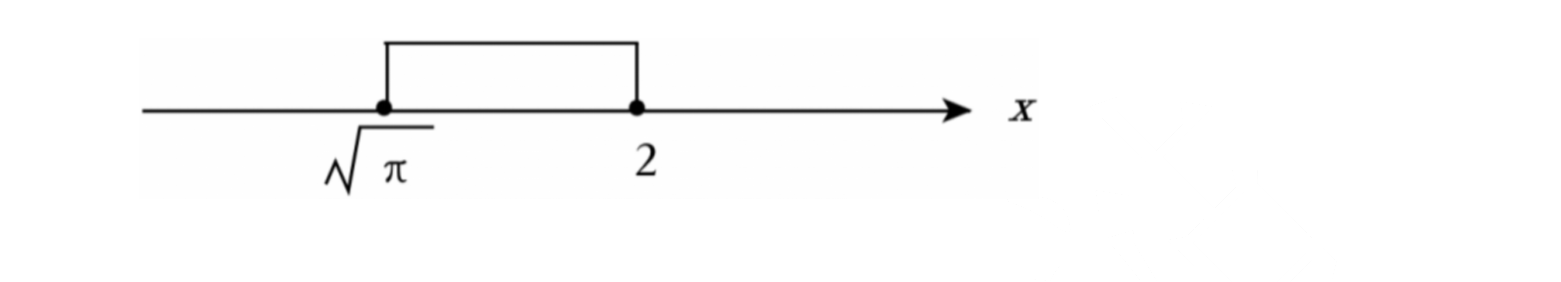
\includegraphics[width=0.72\textwidth]{figures/gao74_q8_numline.png}
\end{center}
\step{所以数形结合得所求集为 $[\sqrt\pi,2]$.}
\solend
\fi

\item 已知集合 $A=\{x\mid(a-1)x^2+3x-3=0,\,x\in\R\}$ 有且仅有一个真子集，则实数 $a=$\blankline[4.4em].

\ifanswer
\solbegin
\step{因为集合 $A=\{x\mid(a-1)x^2+3x-3=0,\,x\in\R\}$ 有且仅有一个真子集，}
\step{所以 $(a-1)x^2+3x-3=0$ 只有一个解，}
\step{所以 $a=1$ 或 $\begin{cases}a\neq1\\ \Delta=3^2-4(a-1)\times(-3)=0\end{cases}$，解得 $a=1$ 或 $a=\dfrac14$.}
\solend
\fi

\item 已知全集 $U=\{(x,y)\mid x,y\in\R\}$，若集合 $A\subseteq U$，且对任意 $(x_1,y_1)\in A$，均存在 $(x_2,y_2)\in A$，使得 $x_1y_2+x_2y_1=0$，则称集合 $A$ 为“对称对点集”. 给出如下集合：

（1）$A=\{(x,y)\mid x,y\in\Z\}$；

（2）$A=\left\{(x,y)\,\middle|\,y=\begin{cases}x+1,&x\geqslant0\\ -x+1,&x<0\end{cases},\ x\in\R,\ x\neq0\right\}$；

（3）$A=\{(x,y)\mid y=x+2,\,x\in\R\}$；

（4）$A=\left\{(x,y)\,\middle|\,y=\dfrac1x,\ x\in\R,\ x\neq0\right\}$.

其中是“对称对点集”的序号为\blankline[4.4em]（写出所有正确的序号）.

\ifanswer
\solbegin
\stepm{(1)}{因为 $0\in\Z$，所以 $(0,0)\in A$.}
\step{对任意 $(x_1,y_1)\in A$，取 $(x_2,y_2)=(0,0)\in A$，}
\step{都有 $x_1\times0+0\times y_1=0$，所以（1）是对称对点集.}
\stepm{(2)}{当 $x_1>0$ 时 $y_1=x_1+1$，取 $x_2=-x_1<0$、$y_2=-x_2+1=x_1+1=y_1$，}
\step{则 $(x_2,y_2)\in A$，且 $x_1y_2+x_2y_1=x_1y_1-x_1y_1=0$；}
\step{当 $x_1<0$ 时同理取 $x_2=-x_1>0$、$y_2=x_2+1=y_1$，}
\step{也有 $(x_2,y_2)\in A$ 且 $x_1y_2+x_2y_1=0$；所以（2）是对称对点集.}
\stepm{(3)}{取 $A$ 中的点 $(-1,1)$. 若存在 $(x_2,y_2)\in A$ 使 $(-1)\cdot y_2+x_2\cdot1=0$，}
\step{则 $y_2=x_2$，但 $A$ 中点的坐标满足 $y=x+2$，两者矛盾，}
\step{所以（3）不是对称对点集.}
\stepm{(4)}{设 $(x_1,y_1)\in A$，则 $x_1\neq0$ 且 $y_1=\dfrac1{x_1}$，}
\step{若存在 $(x_2,y_2)\in A$ 使 $x_1y_2+x_2y_1=0$，}
\step{把 $y_1=\dfrac1{x_1}$、$y_2=\dfrac1{x_2}$（$x_2\neq0$）代入得 $\dfrac{x_1}{x_2}+\dfrac{x_2}{x_1}=0$，即 $x_1^2+x_2^2=0$，}
\step{于是 $x_1=x_2=0$，与 $x_1\neq0$、$x_2\neq0$ 矛盾，所以（4）不是对称对点集.}
\step{故正确的是①②.}
\solend
\fi

\end{enumerate}

\bigsec{二、选择题}

\begin{enumerate}
\setcounter{enumi}{10}

\item “$x>3$”是“$\dfrac{x-1}{x-3}>0$”的\mbox{（\quad）}

\keepwithprev
A. 充分不必要条件\qquad B. 必要不充分条件\qquad C. 充要条件\qquad D. 既不充分也不必要条件

\ifanswer
\solbegin
\step{由 $\dfrac{x-1}{x-3}>0$ 得 $x>3$ 或 $x<1$，故“$x>3$”是“$\dfrac{x-1}{x-3}>0$”的充分不必要条件.}
\step{故选 $A$.}
\solend
\fi

\item 已知 $a,b,c\in\R$，$b>c$，则下列不等式中恒成立的是\mbox{（\quad）}

\keepwithprev
A. $a+b^2>a+c^2$\qquad B. $a^2+b>a^2+c$\qquad C. $ab^2>ac^2$\qquad D. $a^2b>a^2c$

\ifanswer
\solbegin
\step{对于 $A$，取 $b=1,c=-1$，错误；对于 $B$，由不等式的同向可加性得正确；}
\step{对于 $C$，取 $a=1,b=1,c=-2$，错误；对于 $D$，取 $a=0$，错误.}
\step{故选 $B$.}
\solend
\fi

\item 已知关于 $x$ 的不等式 $x^2-2kx+1>0$ 对于一切实数 $x$ 都成立，则实数 $k$ 的取值范围是\mbox{（\quad）}

\keepwithprev
A. $[-1,1]$\qquad B. $(-1,1)$\qquad C. $(-\infty,-1)\cup(1,+\infty)$\qquad D. $\left(-\dfrac12,\dfrac12\right)$

\ifanswer
\solbegin
\step{因为关于 $x$ 的不等式 $x^2-2kx+1>0$ 对于一切实数 $x$ 都成立，}
\step{所以 $\Delta=(-2k)^2-4<0$，即 $4k^2-4<0$，解得 $-1<k<1$，}
\step{所以实数 $k$ 的取值范围是 $(-1,1)$. 故选 $B$.}
\solend
\fi

\item 某种生产设备购买时费用 $100$ 千元，每年的设备管理费 $8$ 千元，这种生产设备的维修费前 $x(x\in\N)$ 年共 $\dfrac{25}{36}x^2+2x$ 千元，问这种生产设备最多使用\mbox{（\quad）}年报废最合算？（即年平均费用最少）

\keepwithprev
A. $13$\qquad B. $10$\qquad C. $15$\qquad D. $12$

\ifanswer
\solbegin
\step{设使用 $x$ 年报废，则总费用 $S(x)=100+8x+\dfrac{25}{36}x^2+2x=\dfrac{25}{36}x^2+10x+100$，}
\step{则年平均费用为 $y=\dfrac{S(x)}x=\dfrac{25x}{36}+\dfrac{100}x+10\geqslant2\sqrt{\dfrac{25x}{36}\cdot\dfrac{100}x}+10=\dfrac{80}3$，}
\step{当且仅当 $\dfrac{25x}{36}=\dfrac{100}x$，即 $x=12$ 时，取等号，}
\step{故当使用 $12$ 年报废，年平均费用最少. 故选 $D$.}
\solend
\fi

\end{enumerate}

\bigsec{三、解答题}

\begin{enumerate}
\setcounter{enumi}{14}

\item （1）设集合 $A=\{x\mid ax-1=0,\,x\in\R\}$，$B=\{x\mid x^2-3x+2=0,\,x\in\R\}$，若 $A\cap B\neq\varnothing$，求实数 $a$ 的取值范围；

（2）已知一元二次方程 $x^2-mx+m+1=0$ 的两个不等实根为 $x_1$、$x_2$，且 $x_1^2+x_2^2=1$，求实数 $m$ 的值.

\ifanswer
\solbegin
\stepm{(1)}{$B=\{x\mid x^2-3x+2=0,\,x\in\R\}=\{1,2\}$，}
\step{①当 $a=0$ 时，方程 $0\cdot x-1=0$ 无解，$A=\varnothing$，$A\cap B=\varnothing$，不符合题意；}
\step{②当 $a\neq0$ 时，$A=\left\{\dfrac1a\right\}$. $A\cap B\neq\varnothing$，}
\step{则 $\dfrac1a\in B$，即 $\dfrac1a=1$ 或 $\dfrac1a=2$，解得 $a=1$ 或 $\dfrac12$；}
\stepm{(2)}{方程 $x^2-mx+m+1=0$ 有两个不等实根，}
\step{则 $\Delta=m^2-4(m+1)>0$，解得 $m>2+2\sqrt2$ 或 $m<2-2\sqrt2$，}
\step{由韦达定理得 $x_1+x_2=m$，$x_1x_2=m+1$，$x_1^2+x_2^2=1$，}
\step{则 $(x_1+x_2)^2-2x_1x_2=m^2-2(m+1)=1$，解得 $m=-1$ 或 $m=3$（舍去），}
\step{综上所述，$m=-1$.}
\solend
\fi

\ansspace

\item 设全集为 $\R$，已知集合 $A=\{x\mid|x-1|\leqslant3,\,x\in\R\}$，

$B=\{x\mid x^2-2mx+(m-3)(m+3)\leqslant0,\,x\in\R\}$.

（1）若 $A\cap B=[0,4]$，求实数 $m$ 的值；

（2）若 $A\cap\overline{B}=A$，求实数 $m$ 的取值范围.

\ifanswer
\solbegin
\stepm{(1)}{$A=\{x\mid|x-1|\leqslant3\}=\{x\mid-2\leqslant x\leqslant4\}$，}
\step{$B=\{x\mid x^2-2mx+(m-3)(m+3)\leqslant0\}=\{x\mid m-3\leqslant x\leqslant m+3\}$，}
\step{若 $A\cap B=[0,4]$，则 $m-3=0$，即 $m=3$；}
\stepm{(2)}{若 $A\cap\overline{B}=A$，则 $A\subseteq\overline{B}$，$\overline{B}=\{x\mid x>m+3\text{ 或 }x<m-3\}$，}
\step{所以 $m+3<-2$ 或 $m-3>4$，解得 $m<-5$ 或 $m>7$，}
\step{实数 $m$ 的取值范围为 $\{m\mid m<-5\text{ 或 }m>7\}$.}
\solend
\fi

\ansspace

\item （1）已知 $a$、$b$ 为正实数，若 $a+b>4$，试用反证法证明：$\dfrac{a}{b+2}$ 和 $\dfrac{b}{a+2}$ 中至少有一个\mbox{大于 $\dfrac12$}；

（2）设 $x$、$y$ 为正实数，$m=\sqrt{2x}+\sqrt{2y}$，$n=\sqrt{x^2+5xy+y^2}$，试比较 $m$、$n$ 的大小，并说明理由.

\ifanswer
\solbegin
\stepm{(1)}{假设 $\dfrac{a}{b+2}\leqslant\dfrac12$ 且 $\dfrac{b}{a+2}\leqslant\dfrac12$，}
\step{又由 $a$、$b$ 为正实数，则有 $2a\leqslant b+2$ 且 $2b\leqslant a+2$，}
\step{两式相加，有 $2a+2b\leqslant a+b+4$，变形得 $a+b\leqslant4$，}
\step{与已知 $a+b>4$ 相矛盾，即假设 $\dfrac{a}{b+2}\leqslant\dfrac12$ 且 $\dfrac{b}{a+2}\leqslant\dfrac12$ 不成立，}
\step{故 $\dfrac{a}{b+2}$ 和 $\dfrac{b}{a+2}$ 中至少有一个\mbox{大于 $\dfrac12$}；}
\stepm{(2)}{$m>n$，理由：$x$、$y$ 为正实数，$m=\sqrt{2x}+\sqrt{2y}$，$n=\sqrt{x^2+5xy+y^2}$，}
\step{则 $m^2=(\sqrt{2x}+\sqrt{2y})^2=2x^2+2y^2+4xy$，$n^2=x^2+y^2+5xy$，}
\step{则有 $m^2-n^2=2x^2+2y^2+4xy-x^2-y^2-5xy=x^2+y^2-xy$}
\step{$=\left(x-\dfrac y2\right)^2+\dfrac{3y^2}4$，}
\step{又 $x$、$y$ 为正实数，则 $m^2-n^2>0$，即 $m^2>n^2$，必有 $m>n$，结论成立.}
\solend
\fi

\ansspace

\item 已知集合 $A=\{a_1,a_2,a_3,\cdots,a_n\}$，$a_i$ 为正整数（$i=1,2,\cdots,n$）.

（1）设 $n=3$，$a_1=1$，$a_2=3$，$a_3=9$，$B=\{a_i+a_j\mid1\leqslant i<j\leqslant3,\,i,j\in\N^*\}$，若互不相同的三个实数 $b_1$、$b_2$、$b_3$，满足 $\{b_i+b_j\mid1\leqslant i<j\leqslant3,\,i,j\in\N^*\}=B$，求有序数组 $(b_1,b_2,b_3)$；

（2）设 $n=4$，$C=\{a_1^2,a_2^2,a_3^2,a_4^2\}$，其中 $a_1<a_2<a_3<a_4$，$A\cap C=\{a_1,a_4\}$，且 $a_1+a_4=10$，$A\cup C$ 中所有元素之和为 $124$，求集合 $A$；

（3）设 $n=2$，有 $7$ 个互不相同的集合 $A$ 分别记为 $A_1$、$A_2$、$A_3$、$\cdots$、$A_7$，且 $A_1\cap A_7=\varnothing$、$A_i\cap A_{i+1}=\varnothing\,(i=1,2,3,\cdots,6)$，记 $D=A_1\cup A_2\cup A_3\cup\cdots\cup A_7$，求 $D$ 中元素个数的最小值.

\ifanswer
\solbegin
\stepm{(1)}{$B=\{a_i+a_j\mid1\leqslant i<j\leqslant3,\,i,j\in\N^*\}=\{1+3,1+9,3+9\}=\{4,10,12\}$，}
\step{由题意，不妨设 $b_1<b_2<b_3$，}
\step{则三个数两两之和为 $\begin{cases}b_1+b_2=4\\ b_1+b_3=10\\ b_2+b_3=12\end{cases}$，解得 $\begin{cases}b_1=1\\ b_2=3\\ b_3=9\end{cases}$，}
\step{所以满足条件的有序数组为 $1$，$3$，$9$ 三个数字的全部排列，}
\step{所以有序数组 $(b_1,b_2,b_3)$ 为 $(1,3,9),(1,9,3),(3,1,9),(3,9,1),(9,1,3),(9,3,1)$；}
\stepm{(2)}{因为 $A\cap C=\{a_1,a_4\}$，所以 $a_1\in C$，$a_4\in C$，}
\step{所以 $a_1$ 是集合 $A$ 中某个正整数的平方，}
\step{又因为 $a_1$ 是最小的正整数，所以只能是 $a_1=1$，此时满足 $1=1^2$.}
\step{又 $a_1+a_4=10$，所以 $a_4=9$，所以 $9$ 也是集合 $A$ 中某个正整数的平方，}
\step{因为 $3^2=9$，所以 $3\in A$，则有 $a_2=3$ 或 $a_3=3$.}
\step{若 $a_3=3$，则 $A=\{1,a_2,3,9\}$，$C=\{1^2,a_2^2,3^2,9^2\}=\{1,a_2^2,9,81\}$，}
\step{因为 $a_1<a_2<a_3<a_4$，且 $a_2$ 为正整数，所以只能是 $a_2=2$，}
\step{故 $A=\{1,2,3,9\}$，$C=\{1,4,9,81\}$，$A\cap C=\{1,9\}$，符合题意，}
\step{则 $A\cup C=\{1,2,3,4,9,81\}$，此时 $1+2+3+4+9+81=100\neq124$，}
\step{故 $a_3=3$ 不符合题意，所以只能 $a_2=3$，}
\step{故 $A=\{1,3,a_3,9\}$，$C=\{1^2,3^2,a_3^2,9^2\}$，此时 $A\cup C=\{1,3,a_3,9,a_3^2,81\}$，}
\step{则有 $1+3+a_3+9+a_3^2+81=124$，}
\step{即 $a_3^2+a_3-30=(a_3+6)(a_3-5)=0$，解得正整数 $a_3=5$，}
\step{此时 $A=\{1,3,5,9\}$，$C=\{1,9,25,81\}$，$A\cup C=\{1,3,5,9,25,81\}$，}
\step{满足 $A\cap C=\{1,9\}$，$A\cup C$ 中所有元素之和为 $1+3+5+9+25+81=124$，}
\step{故 $A=\{1,3,5,9\}$；}
\stepm{(3)}{当 $n=2$ 时，每个集合 $A_i(i=1,2,\cdots,7)$ 均为含有 $2$ 个元素的二元集合，}
\step{设 $D$ 中元素个数为 $m$，}
\step{若 $m\leqslant4$，从 $m$ 个元素中最多能得到 $\dfrac{4\times3}2=6$ 个不同二元集合，不足 $7$ 个，}
\step{故 $m\leqslant4$ 不可能.}
\step{若 $m=5$，则有 $\dfrac{5\times4}2=10$ 个不同二元集合，数量超过 $7$ 个，符合要求.}
\step{因为 $A_i\cap A_{i+1}=\varnothing(i=1,2,3,\cdots,6)$，$A_1\cap A_7=\varnothing$，}
\step{即要求 $7$ 个互不相同的二元集合排成环，}
\step{且相邻（含首尾）集合交集为空集.}
\needvspace{12\baselineskip}
\step{假设 $m=5$，不妨设 $A_1(1,2)$、$A_2(3,4)$、$A_3(1,5)$，则：}
\begin{center}
\renewcommand{\arraystretch}{1.9}
\begin{tabular}{|c|c|c|c|c|}
\hline
$A_4(2,3)$ & $A_5(1,4)$ & $A_6(2,5)$ & $A_7(1,3)$ & 与 $A_1$ 矛盾\\
\hline
 &  & $A_6(3,5)$ & $A_7(2,4)$ & 与 $A_1$ 矛盾\\
\hline
 & $A_5(4,5)$ & $A_6(1,3)$ & $A_7(2,5)$ 或 $A_7(2,4)$ & 与 $A_1$ 矛盾\\
\hline
$A_4(2,4)$ & $A_5(1,3)$ & $A_6(2,5)$ & $A_7(1,4)$ & 与 $A_1$ 矛盾\\
\hline
 &  & $A_6(4,5)$ & $A_7(2,3)$ & 与 $A_1$ 矛盾\\
\hline
 & $A_5(3,5)$ & $A_6(1,4)$ & $A_7(2,3)$ 或 $A_7(2,5)$ & 与 $A_1$ 矛盾\\
\hline
\end{tabular}
\end{center}
\step{故 $m=5$ 不可能.}
\step{综上，$m\geqslant6$，取 $D=\{1,2,3,4,5,6\}$，}
\step{令 $A_1=\{1,2\},A_2=\{3,4\},A_3=\{1,5\},A_4=\{2,4\},A_5=\{3,6\},A_6=\{1,4\}$，}
\step{$A_7=\{5,6\}$，此时 $A_1$、$A_2$、$\cdots$、$A_7$ 是 $7$ 个互不相同的二元集合，}
\step{且 $A_1\cap A_2=\varnothing$，$A_2\cap A_3=\varnothing$，$A_3\cap A_4=\varnothing$，$A_4\cap A_5=\varnothing$，}
\step{$A_5\cap A_6=\varnothing$，$A_6\cap A_7=\varnothing$，$A_7\cap A_1=\varnothing$，满足全部条件，}
\step{故 $D$ 中元素个数的最小值为 $6$.}
\solend
\fi

\ansspace*[7]

\end{enumerate}

\end{document}
"
%
% 原始材料：微信公众号“魔都数学加油站”文章，连载“27学年高一74”；
% 原文标题“27学年高一74——2026-2027年上海市宜川中学高一上10月月考”；
% 原文链接：https://mp.weixin.qq.com/s/ymsl2bmkBRY6ZPDiUFCDTA。
% 页面标注发布时间 2026-10-22 21:45（上海）。
% 正文为 9 张 PNG 页（`原图/高一74_宜川中学_10月月考/01..09.png`）：
% 第 1、2、3 页为 4762×6735，其余 6 页为 2560×3620，均按页序读取。
% 9 页全为试卷正文页（卷首标题在第 1 页页顶，卷末第 18 题 (3) 解析止于第 9 页），
% 无封面页、目录页、二维码或宣传页。粉色斜排“魔都数学加油站”为卷面水印，未录入。
%
% 卷首标题：照卷面印作“2026-2027 年宜川中学高一上 10 月月考”（黑体加粗一行）。
% 原卷年份区间用半角连字符，本稿按全稿惯例排 en dash；原卷无副标题。
%
% 篇幅与题号：原卷自第 3 题起编号（第 1、2 题不在本卷内）。填空题 3—10（8 题）、
% 选择题 11—14（4 题）、解答题 15—18（4 题），共 16 题。本稿沿用原节与原题号，
% 只改排为全稿统一的大节样式。
%
% 讲评版：原卷第 3 题只印【答案】（“{(1,1)}”），本稿只给 \ans{}；其余 15 题均印
% 【解析】，用 \solbegin…\solend。四道选择题的作答括号原卷即留空，答案写在解析末句
% “故选 A／B／B／D”，照录在解析内，不另提 \ans{}。
%
% 副标题：原卷未印副标题。本稿按“知识模块”口径标作“集合与常用逻辑用语、不等式”：
% 16 题中集合与常用逻辑用语 7 题（第 3、9、10、15、16、18 题及第 17 题的反证法），
% 不等式 9 题（第 4—8、11—14、17 题），两类均确有分量，故并标。口径同 高一63、高一68—73。
%
% 与原卷的排版差异：
%   ① 原卷每题下直接印【答案】/【解析】，本稿按全稿惯例将答案与解析置于答案版；
%   ② 原卷未印副标题，本稿按“知识模块”口径补出；
%   ③ 原卷填空横线约四个字宽，本稿按全稿惯例统一排 \blankline[4.4em]；
%   ④ 原卷数集记号排斜体 $R$、$Z$、$N$（第 8、9、10、14—18 题），本稿按全稿惯例
%      改用 $\R$、$\Z$、$\N$（同 高一68—73）；第 18 题的正整数集合作 $\N^*$，照录；
%   ⑤ 原卷句末标点多为西文句点，均逐处照录；
%   ⑥ 第 15—18 题的子问原卷印作“（1）…（2）…”，本稿按 高一69—73 成例用行内
%      “（1）（2）（3）”段，解析中的子问标号用 \stepm{(1)}{…}；
%   ⑦ 每道解答题原卷未留作答空白，本稿按全稿惯例加 \ansspace（末题用 \ansspace*）；
%   ⑧ 选择题的作答括号原卷排半角“(    )”，本稿按全稿惯例排 \mbox{（\quad）}；
%      选项行排照原卷——第 11、13 题一行四条，第 12、14 题一行四条；
%   ⑨ 第 9、14、18 题解析中的不等式组／方程组，原卷均排作“{”连接的多行式，
%      本稿按全稿惯例排 cases；
%   ⑩ 第 8 题解析有一幅数轴图：原卷印在【解析】第 2 行之后，题干无“如图”二字。
%      本稿按原卷截图裁取（`figures/gao74_q8_numline.png`，由第 2 页原图裁出、
%      去除粉色水印后转灰度，未放大），放在答案版解析第 2 条之后；
%   ⑪ 第 18 题 (3) 解析中有一张 5 列 6 行的枚举表（原卷无表头、左侧两列留空以表示
%      沿用上格的 $A_4$／$A_5$），本稿照原卷排成同样的空格表，未加表头、未合并单元格。
%
% 原卷笔误/存疑（均照录未改，正文对应处另有 % 注）：
%   ① 第 14 题题干“维修费前 $x(x\in N)$ 年共 $\dfrac{25}{36}x^2+2x$ 千元”中的
%      $N$ 原卷排斜体，按全稿惯例改 $\N$，含义不变；
%   ② 第 18 题 (3) 的枚举表第 1—3 行与第 4—6 行分属“$A_5(1,4)$”“$A_5(1,3)$”两种
%      情形，原卷只在首行重复写 $A_4$、$A_5$，其余留空；本稿照录留空，未补字。
%
% 行数核对：逐题数 \step/\stepm 条数与原卷【解析】印刷行数，15 题逐一相符，
% 合计 104 条 / 104 行（Q4：1；Q5：2；Q6：3；Q7：3；Q8：3；Q9：3；Q10：15；
% Q11：2；Q12：3；Q13：3；Q14：4；Q15：9；Q16：6；Q17：10；Q18：37）。
% 另第 3 题只印【答案】，提 \ans{}，不计入 \step 账。
%
% 插图：第 8 题解析的数轴图，见上⑩；全卷题干无其他配图。
%
\documentclass[a4paper,11pt]{article}
\usepackage{common}

\begin{document}

\examtitlest[3]{2026--2027 年宜川中学高一上 10 月月考}{集合与常用逻辑用语、不等式}

\bigsec{一、填空题}

\begin{enumerate}
\setcounter{enumi}{2}

\item 已知集合 $A=\{(x,y)\mid y=x\}$，集合 $B=\{(x,y)\mid y=2-x\}$，则 $A\cap B=$\blankline[4.4em].

\ifanswer
\ans{$\{(1,1)\}$}
\fi

\item 已知 $a=\log_3 2$，$b=\log_3 8$，则 $3^{2a-b}=$\blankline[4.4em].

\ifanswer
\solbegin
\step{由 $a=\log_3 2$，$b=\log_3 8$，得 $3^a=2$，$3^b=8$，则 $3^{2a-b}=\dfrac{(3^a)^2}{3^b}=\dfrac48=\dfrac12$.}
\solend
\fi

\item 已知等式 $2x^2+3x+5=a(2x+1)(x+1)+c$ 恒成立，则实数 $c=$\blankline[4.4em].

\ifanswer
\solbegin
\step{$2x^2+3x+5=a(2x+1)(x+1)+c=2ax^2+3ax+a+c$，}
\step{则 $\begin{cases}2a=2\\ 3a=3\\ a+c=5\end{cases}$，解得 $c=4$.}
\solend
\fi

\item 已知 $x>0$，$y>0$，且 $\dfrac9x+\dfrac1y=1$，则 $x\cdot y$ 的最小值是\blankline[4.4em].

\ifanswer
\solbegin
\step{$x>0$，$y>0$，且 $1=\dfrac9x+\dfrac1y\geqslant2\sqrt{\dfrac9{xy}}$，}
\step{当且仅当 $x=9y$，即 $y=2$，$x=18$ 时取等号，所以 $xy\geqslant36$，}
\step{则 $x\cdot y$ 的最小值为 $36$.}
\solend
\fi

\item 已知关于 $x$ 的不等式 $x^2+bx+c>0$（$b$、$c$ 为实数）的解集为 $(-\infty,-2)\cup(3,+\infty)$，则不等式 $cx^2-bx+1\leqslant0$ 的解集为\blankline[4.4em].

\ifanswer
\solbegin
\step{由已知得 $-2$、$3$ 为方程 $x^2+bx+c=0$ 的根，所以 $-2+3=-b$，$-2\times3=c$，}
\step{即 $b=-1$，$c=-6$，所以不等式 $cx^2-bx+1\leqslant0$ 可变形为 $-6x^2+x+1\leqslant0$，}
\step{即 $6x^2-x-1\geqslant0$，解得 $x\leqslant-\dfrac13$ 或 $x\geqslant\dfrac12$，所以解集为 $\left(-\infty,-\dfrac13\right]\cup\left[\dfrac12,+\infty\right)$.}
\solend
\fi

\item 设 $x\in\R$，则方程 $|x-2|+|\sqrt\pi-x|=2-\sqrt\pi$ 的解集为\blankline[4.4em].

\ifanswer
\solbegin
\step{因为方程 $|x-2|+|\sqrt\pi-x|=2-\sqrt\pi$ 可化为 $|x-2|+|x-\sqrt\pi|=2-\sqrt\pi$，}
\needvspace{8\baselineskip}
\step{其表示数轴上实数 $x$ 到 $\sqrt\pi$ 与 $2$ 的距离之和等于 $2-\sqrt\pi$，如图：}
\begin{center}
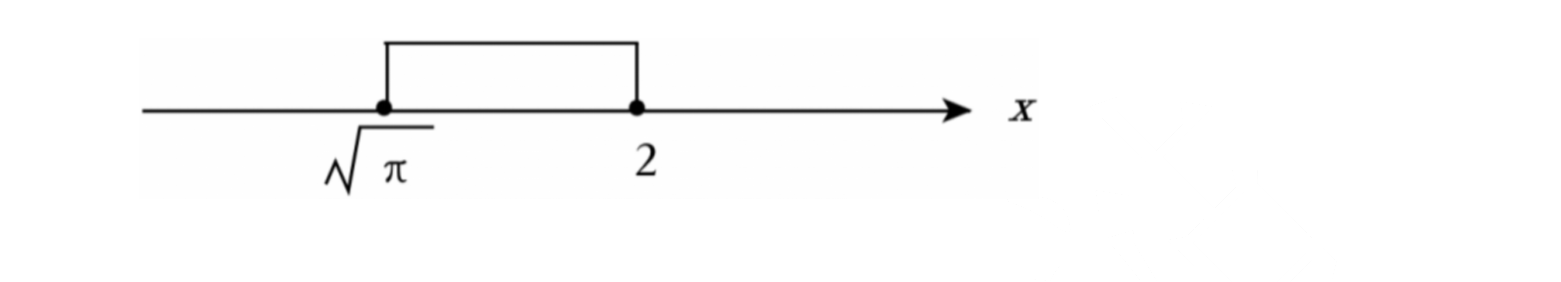
\includegraphics[width=0.72\textwidth]{figures/gao74_q8_numline.png}
\end{center}
\step{所以数形结合得所求集为 $[\sqrt\pi,2]$.}
\solend
\fi

\item 已知集合 $A=\{x\mid(a-1)x^2+3x-3=0,\,x\in\R\}$ 有且仅有一个真子集，则实数 $a=$\blankline[4.4em].

\ifanswer
\solbegin
\step{因为集合 $A=\{x\mid(a-1)x^2+3x-3=0,\,x\in\R\}$ 有且仅有一个真子集，}
\step{所以 $(a-1)x^2+3x-3=0$ 只有一个解，}
\step{所以 $a=1$ 或 $\begin{cases}a\neq1\\ \Delta=3^2-4(a-1)\times(-3)=0\end{cases}$，解得 $a=1$ 或 $a=\dfrac14$.}
\solend
\fi

\item 已知全集 $U=\{(x,y)\mid x,y\in\R\}$，若集合 $A\subseteq U$，且对任意 $(x_1,y_1)\in A$，均存在 $(x_2,y_2)\in A$，使得 $x_1y_2+x_2y_1=0$，则称集合 $A$ 为“对称对点集”. 给出如下集合：

（1）$A=\{(x,y)\mid x,y\in\Z\}$；

（2）$A=\left\{(x,y)\,\middle|\,y=\begin{cases}x+1,&x\geqslant0\\ -x+1,&x<0\end{cases},\ x\in\R,\ x\neq0\right\}$；

（3）$A=\{(x,y)\mid y=x+2,\,x\in\R\}$；

（4）$A=\left\{(x,y)\,\middle|\,y=\dfrac1x,\ x\in\R,\ x\neq0\right\}$.

其中是“对称对点集”的序号为\blankline[4.4em]（写出所有正确的序号）.

\ifanswer
\solbegin
\stepm{(1)}{因为 $0\in\Z$，所以 $(0,0)\in A$.}
\step{对任意 $(x_1,y_1)\in A$，取 $(x_2,y_2)=(0,0)\in A$，}
\step{都有 $x_1\times0+0\times y_1=0$，所以（1）是对称对点集.}
\stepm{(2)}{当 $x_1>0$ 时 $y_1=x_1+1$，取 $x_2=-x_1<0$、$y_2=-x_2+1=x_1+1=y_1$，}
\step{则 $(x_2,y_2)\in A$，且 $x_1y_2+x_2y_1=x_1y_1-x_1y_1=0$；}
\step{当 $x_1<0$ 时同理取 $x_2=-x_1>0$、$y_2=x_2+1=y_1$，}
\step{也有 $(x_2,y_2)\in A$ 且 $x_1y_2+x_2y_1=0$；所以（2）是对称对点集.}
\stepm{(3)}{取 $A$ 中的点 $(-1,1)$. 若存在 $(x_2,y_2)\in A$ 使 $(-1)\cdot y_2+x_2\cdot1=0$，}
\step{则 $y_2=x_2$，但 $A$ 中点的坐标满足 $y=x+2$，两者矛盾，}
\step{所以（3）不是对称对点集.}
\stepm{(4)}{设 $(x_1,y_1)\in A$，则 $x_1\neq0$ 且 $y_1=\dfrac1{x_1}$，}
\step{若存在 $(x_2,y_2)\in A$ 使 $x_1y_2+x_2y_1=0$，}
\step{把 $y_1=\dfrac1{x_1}$、$y_2=\dfrac1{x_2}$（$x_2\neq0$）代入得 $\dfrac{x_1}{x_2}+\dfrac{x_2}{x_1}=0$，即 $x_1^2+x_2^2=0$，}
\step{于是 $x_1=x_2=0$，与 $x_1\neq0$、$x_2\neq0$ 矛盾，所以（4）不是对称对点集.}
\step{故正确的是①②.}
\solend
\fi

\end{enumerate}

\bigsec{二、选择题}

\begin{enumerate}
\setcounter{enumi}{10}

\item “$x>3$”是“$\dfrac{x-1}{x-3}>0$”的\mbox{（\quad）}

\keepwithprev
A. 充分不必要条件\qquad B. 必要不充分条件\qquad C. 充要条件\qquad D. 既不充分也不必要条件

\ifanswer
\solbegin
\step{由 $\dfrac{x-1}{x-3}>0$ 得 $x>3$ 或 $x<1$，故“$x>3$”是“$\dfrac{x-1}{x-3}>0$”的充分不必要条件.}
\step{故选 $A$.}
\solend
\fi

\item 已知 $a,b,c\in\R$，$b>c$，则下列不等式中恒成立的是\mbox{（\quad）}

\keepwithprev
A. $a+b^2>a+c^2$\qquad B. $a^2+b>a^2+c$\qquad C. $ab^2>ac^2$\qquad D. $a^2b>a^2c$

\ifanswer
\solbegin
\step{对于 $A$，取 $b=1,c=-1$，错误；对于 $B$，由不等式的同向可加性得正确；}
\step{对于 $C$，取 $a=1,b=1,c=-2$，错误；对于 $D$，取 $a=0$，错误.}
\step{故选 $B$.}
\solend
\fi

\item 已知关于 $x$ 的不等式 $x^2-2kx+1>0$ 对于一切实数 $x$ 都成立，则实数 $k$ 的取值范围是\mbox{（\quad）}

\keepwithprev
A. $[-1,1]$\qquad B. $(-1,1)$\qquad C. $(-\infty,-1)\cup(1,+\infty)$\qquad D. $\left(-\dfrac12,\dfrac12\right)$

\ifanswer
\solbegin
\step{因为关于 $x$ 的不等式 $x^2-2kx+1>0$ 对于一切实数 $x$ 都成立，}
\step{所以 $\Delta=(-2k)^2-4<0$，即 $4k^2-4<0$，解得 $-1<k<1$，}
\step{所以实数 $k$ 的取值范围是 $(-1,1)$. 故选 $B$.}
\solend
\fi

\item 某种生产设备购买时费用 $100$ 千元，每年的设备管理费 $8$ 千元，这种生产设备的维修费前 $x(x\in\N)$ 年共 $\dfrac{25}{36}x^2+2x$ 千元，问这种生产设备最多使用\mbox{（\quad）}年报废最合算？（即年平均费用最少）

\keepwithprev
A. $13$\qquad B. $10$\qquad C. $15$\qquad D. $12$

\ifanswer
\solbegin
\step{设使用 $x$ 年报废，则总费用 $S(x)=100+8x+\dfrac{25}{36}x^2+2x=\dfrac{25}{36}x^2+10x+100$，}
\step{则年平均费用为 $y=\dfrac{S(x)}x=\dfrac{25x}{36}+\dfrac{100}x+10\geqslant2\sqrt{\dfrac{25x}{36}\cdot\dfrac{100}x}+10=\dfrac{80}3$，}
\step{当且仅当 $\dfrac{25x}{36}=\dfrac{100}x$，即 $x=12$ 时，取等号，}
\step{故当使用 $12$ 年报废，年平均费用最少. 故选 $D$.}
\solend
\fi

\end{enumerate}

\bigsec{三、解答题}

\begin{enumerate}
\setcounter{enumi}{14}

\item （1）设集合 $A=\{x\mid ax-1=0,\,x\in\R\}$，$B=\{x\mid x^2-3x+2=0,\,x\in\R\}$，若 $A\cap B\neq\varnothing$，求实数 $a$ 的取值范围；

（2）已知一元二次方程 $x^2-mx+m+1=0$ 的两个不等实根为 $x_1$、$x_2$，且 $x_1^2+x_2^2=1$，求实数 $m$ 的值.

\ifanswer
\solbegin
\stepm{(1)}{$B=\{x\mid x^2-3x+2=0,\,x\in\R\}=\{1,2\}$，}
\step{①当 $a=0$ 时，方程 $0\cdot x-1=0$ 无解，$A=\varnothing$，$A\cap B=\varnothing$，不符合题意；}
\step{②当 $a\neq0$ 时，$A=\left\{\dfrac1a\right\}$. $A\cap B\neq\varnothing$，}
\step{则 $\dfrac1a\in B$，即 $\dfrac1a=1$ 或 $\dfrac1a=2$，解得 $a=1$ 或 $\dfrac12$；}
\stepm{(2)}{方程 $x^2-mx+m+1=0$ 有两个不等实根，}
\step{则 $\Delta=m^2-4(m+1)>0$，解得 $m>2+2\sqrt2$ 或 $m<2-2\sqrt2$，}
\step{由韦达定理得 $x_1+x_2=m$，$x_1x_2=m+1$，$x_1^2+x_2^2=1$，}
\step{则 $(x_1+x_2)^2-2x_1x_2=m^2-2(m+1)=1$，解得 $m=-1$ 或 $m=3$（舍去），}
\step{综上所述，$m=-1$.}
\solend
\fi

\ansspace

\item 设全集为 $\R$，已知集合 $A=\{x\mid|x-1|\leqslant3,\,x\in\R\}$，

$B=\{x\mid x^2-2mx+(m-3)(m+3)\leqslant0,\,x\in\R\}$.

（1）若 $A\cap B=[0,4]$，求实数 $m$ 的值；

（2）若 $A\cap\overline{B}=A$，求实数 $m$ 的取值范围.

\ifanswer
\solbegin
\stepm{(1)}{$A=\{x\mid|x-1|\leqslant3\}=\{x\mid-2\leqslant x\leqslant4\}$，}
\step{$B=\{x\mid x^2-2mx+(m-3)(m+3)\leqslant0\}=\{x\mid m-3\leqslant x\leqslant m+3\}$，}
\step{若 $A\cap B=[0,4]$，则 $m-3=0$，即 $m=3$；}
\stepm{(2)}{若 $A\cap\overline{B}=A$，则 $A\subseteq\overline{B}$，$\overline{B}=\{x\mid x>m+3\text{ 或 }x<m-3\}$，}
\step{所以 $m+3<-2$ 或 $m-3>4$，解得 $m<-5$ 或 $m>7$，}
\step{实数 $m$ 的取值范围为 $\{m\mid m<-5\text{ 或 }m>7\}$.}
\solend
\fi

\ansspace

\item （1）已知 $a$、$b$ 为正实数，若 $a+b>4$，试用反证法证明：$\dfrac{a}{b+2}$ 和 $\dfrac{b}{a+2}$ 中至少有一个\mbox{大于 $\dfrac12$}；

（2）设 $x$、$y$ 为正实数，$m=\sqrt{2x}+\sqrt{2y}$，$n=\sqrt{x^2+5xy+y^2}$，试比较 $m$、$n$ 的大小，并说明理由.

\ifanswer
\solbegin
\stepm{(1)}{假设 $\dfrac{a}{b+2}\leqslant\dfrac12$ 且 $\dfrac{b}{a+2}\leqslant\dfrac12$，}
\step{又由 $a$、$b$ 为正实数，则有 $2a\leqslant b+2$ 且 $2b\leqslant a+2$，}
\step{两式相加，有 $2a+2b\leqslant a+b+4$，变形得 $a+b\leqslant4$，}
\step{与已知 $a+b>4$ 相矛盾，即假设 $\dfrac{a}{b+2}\leqslant\dfrac12$ 且 $\dfrac{b}{a+2}\leqslant\dfrac12$ 不成立，}
\step{故 $\dfrac{a}{b+2}$ 和 $\dfrac{b}{a+2}$ 中至少有一个\mbox{大于 $\dfrac12$}；}
\stepm{(2)}{$m>n$，理由：$x$、$y$ 为正实数，$m=\sqrt{2x}+\sqrt{2y}$，$n=\sqrt{x^2+5xy+y^2}$，}
\step{则 $m^2=(\sqrt{2x}+\sqrt{2y})^2=2x^2+2y^2+4xy$，$n^2=x^2+y^2+5xy$，}
\step{则有 $m^2-n^2=2x^2+2y^2+4xy-x^2-y^2-5xy=x^2+y^2-xy$}
\step{$=\left(x-\dfrac y2\right)^2+\dfrac{3y^2}4$，}
\step{又 $x$、$y$ 为正实数，则 $m^2-n^2>0$，即 $m^2>n^2$，必有 $m>n$，结论成立.}
\solend
\fi

\ansspace

\item 已知集合 $A=\{a_1,a_2,a_3,\cdots,a_n\}$，$a_i$ 为正整数（$i=1,2,\cdots,n$）.

（1）设 $n=3$，$a_1=1$，$a_2=3$，$a_3=9$，$B=\{a_i+a_j\mid1\leqslant i<j\leqslant3,\,i,j\in\N^*\}$，若互不相同的三个实数 $b_1$、$b_2$、$b_3$，满足 $\{b_i+b_j\mid1\leqslant i<j\leqslant3,\,i,j\in\N^*\}=B$，求有序数组 $(b_1,b_2,b_3)$；

（2）设 $n=4$，$C=\{a_1^2,a_2^2,a_3^2,a_4^2\}$，其中 $a_1<a_2<a_3<a_4$，$A\cap C=\{a_1,a_4\}$，且 $a_1+a_4=10$，$A\cup C$ 中所有元素之和为 $124$，求集合 $A$；

（3）设 $n=2$，有 $7$ 个互不相同的集合 $A$ 分别记为 $A_1$、$A_2$、$A_3$、$\cdots$、$A_7$，且 $A_1\cap A_7=\varnothing$、$A_i\cap A_{i+1}=\varnothing\,(i=1,2,3,\cdots,6)$，记 $D=A_1\cup A_2\cup A_3\cup\cdots\cup A_7$，求 $D$ 中元素个数的最小值.

\ifanswer
\solbegin
\stepm{(1)}{$B=\{a_i+a_j\mid1\leqslant i<j\leqslant3,\,i,j\in\N^*\}=\{1+3,1+9,3+9\}=\{4,10,12\}$，}
\step{由题意，不妨设 $b_1<b_2<b_3$，}
\step{则三个数两两之和为 $\begin{cases}b_1+b_2=4\\ b_1+b_3=10\\ b_2+b_3=12\end{cases}$，解得 $\begin{cases}b_1=1\\ b_2=3\\ b_3=9\end{cases}$，}
\step{所以满足条件的有序数组为 $1$，$3$，$9$ 三个数字的全部排列，}
\step{所以有序数组 $(b_1,b_2,b_3)$ 为 $(1,3,9),(1,9,3),(3,1,9),(3,9,1),(9,1,3),(9,3,1)$；}
\stepm{(2)}{因为 $A\cap C=\{a_1,a_4\}$，所以 $a_1\in C$，$a_4\in C$，}
\step{所以 $a_1$ 是集合 $A$ 中某个正整数的平方，}
\step{又因为 $a_1$ 是最小的正整数，所以只能是 $a_1=1$，此时满足 $1=1^2$.}
\step{又 $a_1+a_4=10$，所以 $a_4=9$，所以 $9$ 也是集合 $A$ 中某个正整数的平方，}
\step{因为 $3^2=9$，所以 $3\in A$，则有 $a_2=3$ 或 $a_3=3$.}
\step{若 $a_3=3$，则 $A=\{1,a_2,3,9\}$，$C=\{1^2,a_2^2,3^2,9^2\}=\{1,a_2^2,9,81\}$，}
\step{因为 $a_1<a_2<a_3<a_4$，且 $a_2$ 为正整数，所以只能是 $a_2=2$，}
\step{故 $A=\{1,2,3,9\}$，$C=\{1,4,9,81\}$，$A\cap C=\{1,9\}$，符合题意，}
\step{则 $A\cup C=\{1,2,3,4,9,81\}$，此时 $1+2+3+4+9+81=100\neq124$，}
\step{故 $a_3=3$ 不符合题意，所以只能 $a_2=3$，}
\step{故 $A=\{1,3,a_3,9\}$，$C=\{1^2,3^2,a_3^2,9^2\}$，此时 $A\cup C=\{1,3,a_3,9,a_3^2,81\}$，}
\step{则有 $1+3+a_3+9+a_3^2+81=124$，}
\step{即 $a_3^2+a_3-30=(a_3+6)(a_3-5)=0$，解得正整数 $a_3=5$，}
\step{此时 $A=\{1,3,5,9\}$，$C=\{1,9,25,81\}$，$A\cup C=\{1,3,5,9,25,81\}$，}
\step{满足 $A\cap C=\{1,9\}$，$A\cup C$ 中所有元素之和为 $1+3+5+9+25+81=124$，}
\step{故 $A=\{1,3,5,9\}$；}
\stepm{(3)}{当 $n=2$ 时，每个集合 $A_i(i=1,2,\cdots,7)$ 均为含有 $2$ 个元素的二元集合，}
\step{设 $D$ 中元素个数为 $m$，}
\step{若 $m\leqslant4$，从 $m$ 个元素中最多能得到 $\dfrac{4\times3}2=6$ 个不同二元集合，不足 $7$ 个，}
\step{故 $m\leqslant4$ 不可能.}
\step{若 $m=5$，则有 $\dfrac{5\times4}2=10$ 个不同二元集合，数量超过 $7$ 个，符合要求.}
\step{因为 $A_i\cap A_{i+1}=\varnothing(i=1,2,3,\cdots,6)$，$A_1\cap A_7=\varnothing$，}
\step{即要求 $7$ 个互不相同的二元集合排成环，}
\step{且相邻（含首尾）集合交集为空集.}
\needvspace{12\baselineskip}
\step{假设 $m=5$，不妨设 $A_1(1,2)$、$A_2(3,4)$、$A_3(1,5)$，则：}
\begin{center}
\renewcommand{\arraystretch}{1.9}
\begin{tabular}{|c|c|c|c|c|}
\hline
$A_4(2,3)$ & $A_5(1,4)$ & $A_6(2,5)$ & $A_7(1,3)$ & 与 $A_1$ 矛盾\\
\hline
 &  & $A_6(3,5)$ & $A_7(2,4)$ & 与 $A_1$ 矛盾\\
\hline
 & $A_5(4,5)$ & $A_6(1,3)$ & $A_7(2,5)$ 或 $A_7(2,4)$ & 与 $A_1$ 矛盾\\
\hline
$A_4(2,4)$ & $A_5(1,3)$ & $A_6(2,5)$ & $A_7(1,4)$ & 与 $A_1$ 矛盾\\
\hline
 &  & $A_6(4,5)$ & $A_7(2,3)$ & 与 $A_1$ 矛盾\\
\hline
 & $A_5(3,5)$ & $A_6(1,4)$ & $A_7(2,3)$ 或 $A_7(2,5)$ & 与 $A_1$ 矛盾\\
\hline
\end{tabular}
\end{center}
\step{故 $m=5$ 不可能.}
\step{综上，$m\geqslant6$，取 $D=\{1,2,3,4,5,6\}$，}
\step{令 $A_1=\{1,2\},A_2=\{3,4\},A_3=\{1,5\},A_4=\{2,4\},A_5=\{3,6\},A_6=\{1,4\}$，}
\step{$A_7=\{5,6\}$，此时 $A_1$、$A_2$、$\cdots$、$A_7$ 是 $7$ 个互不相同的二元集合，}
\step{且 $A_1\cap A_2=\varnothing$，$A_2\cap A_3=\varnothing$，$A_3\cap A_4=\varnothing$，$A_4\cap A_5=\varnothing$，}
\step{$A_5\cap A_6=\varnothing$，$A_6\cap A_7=\varnothing$，$A_7\cap A_1=\varnothing$，满足全部条件，}
\step{故 $D$ 中元素个数的最小值为 $6$.}
\solend
\fi

\ansspace*[7]

\end{enumerate}

\end{document}
"
%
% 原始材料：微信公众号“魔都数学加油站”文章，连载“27学年高一74”；
% 原文标题“27学年高一74——2026-2027年上海市宜川中学高一上10月月考”；
% 原文链接：https://mp.weixin.qq.com/s/ymsl2bmkBRY6ZPDiUFCDTA。
% 页面标注发布时间 2026-10-22 21:45（上海）。
% 正文为 9 张 PNG 页（`原图/高一74_宜川中学_10月月考/01..09.png`）：
% 第 1、2、3 页为 4762×6735，其余 6 页为 2560×3620，均按页序读取。
% 9 页全为试卷正文页（卷首标题在第 1 页页顶，卷末第 18 题 (3) 解析止于第 9 页），
% 无封面页、目录页、二维码或宣传页。粉色斜排“魔都数学加油站”为卷面水印，未录入。
%
% 卷首标题：照卷面印作“2026-2027 年宜川中学高一上 10 月月考”（黑体加粗一行）。
% 原卷年份区间用半角连字符，本稿按全稿惯例排 en dash；原卷无副标题。
%
% 篇幅与题号：原卷自第 3 题起编号（第 1、2 题不在本卷内）。填空题 3—10（8 题）、
% 选择题 11—14（4 题）、解答题 15—18（4 题），共 16 题。本稿沿用原节与原题号，
% 只改排为全稿统一的大节样式。
%
% 讲评版：原卷第 3 题只印【答案】（“{(1,1)}”），本稿只给 \ans{}；其余 15 题均印
% 【解析】，用 \solbegin…\solend。四道选择题的作答括号原卷即留空，答案写在解析末句
% “故选 A／B／B／D”，照录在解析内，不另提 \ans{}。
%
% 副标题：原卷未印副标题。本稿按“知识模块”口径标作“集合与常用逻辑用语、不等式”：
% 16 题中集合与常用逻辑用语 7 题（第 3、9、10、15、16、18 题及第 17 题的反证法），
% 不等式 9 题（第 4—8、11—14、17 题），两类均确有分量，故并标。口径同 高一63、高一68—73。
%
% 与原卷的排版差异：
%   ① 原卷每题下直接印【答案】/【解析】，本稿按全稿惯例将答案与解析置于答案版；
%   ② 原卷未印副标题，本稿按“知识模块”口径补出；
%   ③ 原卷填空横线约四个字宽，本稿按全稿惯例统一排 \blankline[4.4em]；
%   ④ 原卷数集记号排斜体 $R$、$Z$、$N$（第 8、9、10、14—18 题），本稿按全稿惯例
%      改用 $\R$、$\Z$、$\N$（同 高一68—73）；第 18 题的正整数集合作 $\N^*$，照录；
%   ⑤ 原卷句末标点多为西文句点，均逐处照录；
%   ⑥ 第 15—18 题的子问原卷印作“（1）…（2）…”，本稿按 高一69—73 成例用行内
%      “（1）（2）（3）”段，解析中的子问标号用 \stepm{(1)}{…}；
%   ⑦ 每道解答题原卷未留作答空白，本稿按全稿惯例加 \ansspace（末题用 \ansspace*）；
%   ⑧ 选择题的作答括号原卷排半角“(    )”，本稿按全稿惯例排 \mbox{（\quad）}；
%      选项行排照原卷——第 11、13 题一行四条，第 12、14 题一行四条；
%   ⑨ 第 9、14、18 题解析中的不等式组／方程组，原卷均排作“{”连接的多行式，
%      本稿按全稿惯例排 cases；
%   ⑩ 第 8 题解析有一幅数轴图：原卷印在【解析】第 2 行之后，题干无“如图”二字。
%      本稿按原卷截图裁取（`figures/gao74_q8_numline.png`，由第 2 页原图裁出、
%      去除粉色水印后转灰度，未放大），放在答案版解析第 2 条之后；
%   ⑪ 第 18 题 (3) 解析中有一张 5 列 6 行的枚举表（原卷无表头、左侧两列留空以表示
%      沿用上格的 $A_4$／$A_5$），本稿照原卷排成同样的空格表，未加表头、未合并单元格。
%
% 原卷笔误/存疑（均照录未改，正文对应处另有 % 注）：
%   ① 第 14 题题干“维修费前 $x(x\in N)$ 年共 $\dfrac{25}{36}x^2+2x$ 千元”中的
%      $N$ 原卷排斜体，按全稿惯例改 $\N$，含义不变；
%   ② 第 18 题 (3) 的枚举表第 1—3 行与第 4—6 行分属“$A_5(1,4)$”“$A_5(1,3)$”两种
%      情形，原卷只在首行重复写 $A_4$、$A_5$，其余留空；本稿照录留空，未补字。
%
% 行数核对：逐题数 \step/\stepm 条数与原卷【解析】印刷行数，15 题逐一相符，
% 合计 104 条 / 104 行（Q4：1；Q5：2；Q6：3；Q7：3；Q8：3；Q9：3；Q10：15；
% Q11：2；Q12：3；Q13：3；Q14：4；Q15：9；Q16：6；Q17：10；Q18：37）。
% 另第 3 题只印【答案】，提 \ans{}，不计入 \step 账。
%
% 插图：第 8 题解析的数轴图，见上⑩；全卷题干无其他配图。
%
\documentclass[a4paper,11pt]{article}
\usepackage{common}

\begin{document}

\examtitlest[3]{2026--2027 年宜川中学高一上 10 月月考}{集合与常用逻辑用语、不等式}

\bigsec{一、填空题}

\begin{enumerate}
\setcounter{enumi}{2}

\item 已知集合 $A=\{(x,y)\mid y=x\}$，集合 $B=\{(x,y)\mid y=2-x\}$，则 $A\cap B=$\blankline[4.4em].

\ifanswer
\ans{$\{(1,1)\}$}
\fi

\item 已知 $a=\log_3 2$，$b=\log_3 8$，则 $3^{2a-b}=$\blankline[4.4em].

\ifanswer
\solbegin
\step{由 $a=\log_3 2$，$b=\log_3 8$，得 $3^a=2$，$3^b=8$，则 $3^{2a-b}=\dfrac{(3^a)^2}{3^b}=\dfrac48=\dfrac12$.}
\solend
\fi

\item 已知等式 $2x^2+3x+5=a(2x+1)(x+1)+c$ 恒成立，则实数 $c=$\blankline[4.4em].

\ifanswer
\solbegin
\step{$2x^2+3x+5=a(2x+1)(x+1)+c=2ax^2+3ax+a+c$，}
\step{则 $\begin{cases}2a=2\\ 3a=3\\ a+c=5\end{cases}$，解得 $c=4$.}
\solend
\fi

\item 已知 $x>0$，$y>0$，且 $\dfrac9x+\dfrac1y=1$，则 $x\cdot y$ 的最小值是\blankline[4.4em].

\ifanswer
\solbegin
\step{$x>0$，$y>0$，且 $1=\dfrac9x+\dfrac1y\geqslant2\sqrt{\dfrac9{xy}}$，}
\step{当且仅当 $x=9y$，即 $y=2$，$x=18$ 时取等号，所以 $xy\geqslant36$，}
\step{则 $x\cdot y$ 的最小值为 $36$.}
\solend
\fi

\item 已知关于 $x$ 的不等式 $x^2+bx+c>0$（$b$、$c$ 为实数）的解集为 $(-\infty,-2)\cup(3,+\infty)$，则不等式 $cx^2-bx+1\leqslant0$ 的解集为\blankline[4.4em].

\ifanswer
\solbegin
\step{由已知得 $-2$、$3$ 为方程 $x^2+bx+c=0$ 的根，所以 $-2+3=-b$，$-2\times3=c$，}
\step{即 $b=-1$，$c=-6$，所以不等式 $cx^2-bx+1\leqslant0$ 可变形为 $-6x^2+x+1\leqslant0$，}
\step{即 $6x^2-x-1\geqslant0$，解得 $x\leqslant-\dfrac13$ 或 $x\geqslant\dfrac12$，所以解集为 $\left(-\infty,-\dfrac13\right]\cup\left[\dfrac12,+\infty\right)$.}
\solend
\fi

\item 设 $x\in\R$，则方程 $|x-2|+|\sqrt\pi-x|=2-\sqrt\pi$ 的解集为\blankline[4.4em].

\ifanswer
\solbegin
\step{因为方程 $|x-2|+|\sqrt\pi-x|=2-\sqrt\pi$ 可化为 $|x-2|+|x-\sqrt\pi|=2-\sqrt\pi$，}
\needvspace{8\baselineskip}
\step{其表示数轴上实数 $x$ 到 $\sqrt\pi$ 与 $2$ 的距离之和等于 $2-\sqrt\pi$，如图：}
\begin{center}
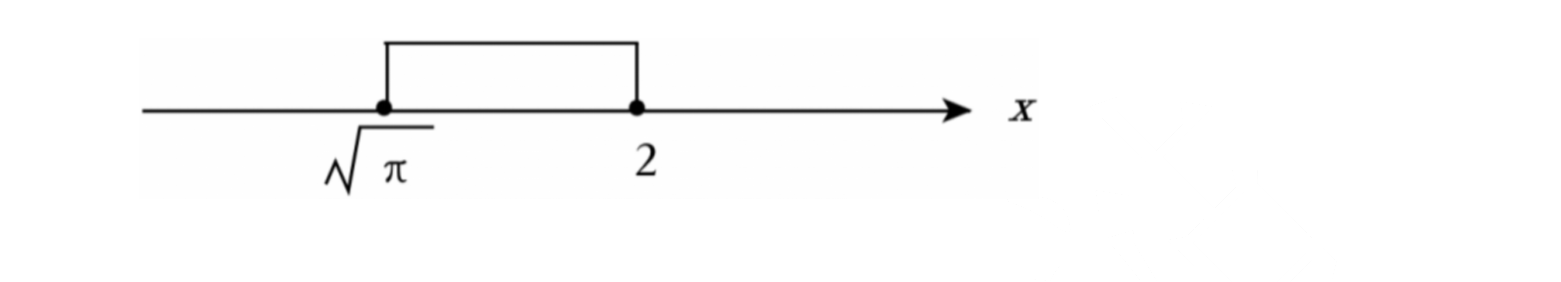
\includegraphics[width=0.72\textwidth]{figures/gao74_q8_numline.png}
\end{center}
\step{所以数形结合得所求集为 $[\sqrt\pi,2]$.}
\solend
\fi

\item 已知集合 $A=\{x\mid(a-1)x^2+3x-3=0,\,x\in\R\}$ 有且仅有一个真子集，则实数 $a=$\blankline[4.4em].

\ifanswer
\solbegin
\step{因为集合 $A=\{x\mid(a-1)x^2+3x-3=0,\,x\in\R\}$ 有且仅有一个真子集，}
\step{所以 $(a-1)x^2+3x-3=0$ 只有一个解，}
\step{所以 $a=1$ 或 $\begin{cases}a\neq1\\ \Delta=3^2-4(a-1)\times(-3)=0\end{cases}$，解得 $a=1$ 或 $a=\dfrac14$.}
\solend
\fi

\item 已知全集 $U=\{(x,y)\mid x,y\in\R\}$，若集合 $A\subseteq U$，且对任意 $(x_1,y_1)\in A$，均存在 $(x_2,y_2)\in A$，使得 $x_1y_2+x_2y_1=0$，则称集合 $A$ 为“对称对点集”. 给出如下集合：

（1）$A=\{(x,y)\mid x,y\in\Z\}$；

（2）$A=\left\{(x,y)\,\middle|\,y=\begin{cases}x+1,&x\geqslant0\\ -x+1,&x<0\end{cases},\ x\in\R,\ x\neq0\right\}$；

（3）$A=\{(x,y)\mid y=x+2,\,x\in\R\}$；

（4）$A=\left\{(x,y)\,\middle|\,y=\dfrac1x,\ x\in\R,\ x\neq0\right\}$.

其中是“对称对点集”的序号为\blankline[4.4em]（写出所有正确的序号）.

\ifanswer
\solbegin
\stepm{(1)}{因为 $0\in\Z$，所以 $(0,0)\in A$.}
\step{对任意 $(x_1,y_1)\in A$，取 $(x_2,y_2)=(0,0)\in A$，}
\step{都有 $x_1\times0+0\times y_1=0$，所以（1）是对称对点集.}
\stepm{(2)}{当 $x_1>0$ 时 $y_1=x_1+1$，取 $x_2=-x_1<0$、$y_2=-x_2+1=x_1+1=y_1$，}
\step{则 $(x_2,y_2)\in A$，且 $x_1y_2+x_2y_1=x_1y_1-x_1y_1=0$；}
\step{当 $x_1<0$ 时同理取 $x_2=-x_1>0$、$y_2=x_2+1=y_1$，}
\step{也有 $(x_2,y_2)\in A$ 且 $x_1y_2+x_2y_1=0$；所以（2）是对称对点集.}
\stepm{(3)}{取 $A$ 中的点 $(-1,1)$. 若存在 $(x_2,y_2)\in A$ 使 $(-1)\cdot y_2+x_2\cdot1=0$，}
\step{则 $y_2=x_2$，但 $A$ 中点的坐标满足 $y=x+2$，两者矛盾，}
\step{所以（3）不是对称对点集.}
\stepm{(4)}{设 $(x_1,y_1)\in A$，则 $x_1\neq0$ 且 $y_1=\dfrac1{x_1}$，}
\step{若存在 $(x_2,y_2)\in A$ 使 $x_1y_2+x_2y_1=0$，}
\step{把 $y_1=\dfrac1{x_1}$、$y_2=\dfrac1{x_2}$（$x_2\neq0$）代入得 $\dfrac{x_1}{x_2}+\dfrac{x_2}{x_1}=0$，即 $x_1^2+x_2^2=0$，}
\step{于是 $x_1=x_2=0$，与 $x_1\neq0$、$x_2\neq0$ 矛盾，所以（4）不是对称对点集.}
\step{故正确的是①②.}
\solend
\fi

\end{enumerate}

\bigsec{二、选择题}

\begin{enumerate}
\setcounter{enumi}{10}

\item “$x>3$”是“$\dfrac{x-1}{x-3}>0$”的\mbox{（\quad）}

\keepwithprev
A. 充分不必要条件\qquad B. 必要不充分条件\qquad C. 充要条件\qquad D. 既不充分也不必要条件

\ifanswer
\solbegin
\step{由 $\dfrac{x-1}{x-3}>0$ 得 $x>3$ 或 $x<1$，故“$x>3$”是“$\dfrac{x-1}{x-3}>0$”的充分不必要条件.}
\step{故选 $A$.}
\solend
\fi

\item 已知 $a,b,c\in\R$，$b>c$，则下列不等式中恒成立的是\mbox{（\quad）}

\keepwithprev
A. $a+b^2>a+c^2$\qquad B. $a^2+b>a^2+c$\qquad C. $ab^2>ac^2$\qquad D. $a^2b>a^2c$

\ifanswer
\solbegin
\step{对于 $A$，取 $b=1,c=-1$，错误；对于 $B$，由不等式的同向可加性得正确；}
\step{对于 $C$，取 $a=1,b=1,c=-2$，错误；对于 $D$，取 $a=0$，错误.}
\step{故选 $B$.}
\solend
\fi

\item 已知关于 $x$ 的不等式 $x^2-2kx+1>0$ 对于一切实数 $x$ 都成立，则实数 $k$ 的取值范围是\mbox{（\quad）}

\keepwithprev
A. $[-1,1]$\qquad B. $(-1,1)$\qquad C. $(-\infty,-1)\cup(1,+\infty)$\qquad D. $\left(-\dfrac12,\dfrac12\right)$

\ifanswer
\solbegin
\step{因为关于 $x$ 的不等式 $x^2-2kx+1>0$ 对于一切实数 $x$ 都成立，}
\step{所以 $\Delta=(-2k)^2-4<0$，即 $4k^2-4<0$，解得 $-1<k<1$，}
\step{所以实数 $k$ 的取值范围是 $(-1,1)$. 故选 $B$.}
\solend
\fi

\item 某种生产设备购买时费用 $100$ 千元，每年的设备管理费 $8$ 千元，这种生产设备的维修费前 $x(x\in\N)$ 年共 $\dfrac{25}{36}x^2+2x$ 千元，问这种生产设备最多使用\mbox{（\quad）}年报废最合算？（即年平均费用最少）

\keepwithprev
A. $13$\qquad B. $10$\qquad C. $15$\qquad D. $12$

\ifanswer
\solbegin
\step{设使用 $x$ 年报废，则总费用 $S(x)=100+8x+\dfrac{25}{36}x^2+2x=\dfrac{25}{36}x^2+10x+100$，}
\step{则年平均费用为 $y=\dfrac{S(x)}x=\dfrac{25x}{36}+\dfrac{100}x+10\geqslant2\sqrt{\dfrac{25x}{36}\cdot\dfrac{100}x}+10=\dfrac{80}3$，}
\step{当且仅当 $\dfrac{25x}{36}=\dfrac{100}x$，即 $x=12$ 时，取等号，}
\step{故当使用 $12$ 年报废，年平均费用最少. 故选 $D$.}
\solend
\fi

\end{enumerate}

\bigsec{三、解答题}

\begin{enumerate}
\setcounter{enumi}{14}

\item （1）设集合 $A=\{x\mid ax-1=0,\,x\in\R\}$，$B=\{x\mid x^2-3x+2=0,\,x\in\R\}$，若 $A\cap B\neq\varnothing$，求实数 $a$ 的取值范围；

（2）已知一元二次方程 $x^2-mx+m+1=0$ 的两个不等实根为 $x_1$、$x_2$，且 $x_1^2+x_2^2=1$，求实数 $m$ 的值.

\ifanswer
\solbegin
\stepm{(1)}{$B=\{x\mid x^2-3x+2=0,\,x\in\R\}=\{1,2\}$，}
\step{①当 $a=0$ 时，方程 $0\cdot x-1=0$ 无解，$A=\varnothing$，$A\cap B=\varnothing$，不符合题意；}
\step{②当 $a\neq0$ 时，$A=\left\{\dfrac1a\right\}$. $A\cap B\neq\varnothing$，}
\step{则 $\dfrac1a\in B$，即 $\dfrac1a=1$ 或 $\dfrac1a=2$，解得 $a=1$ 或 $\dfrac12$；}
\stepm{(2)}{方程 $x^2-mx+m+1=0$ 有两个不等实根，}
\step{则 $\Delta=m^2-4(m+1)>0$，解得 $m>2+2\sqrt2$ 或 $m<2-2\sqrt2$，}
\step{由韦达定理得 $x_1+x_2=m$，$x_1x_2=m+1$，$x_1^2+x_2^2=1$，}
\step{则 $(x_1+x_2)^2-2x_1x_2=m^2-2(m+1)=1$，解得 $m=-1$ 或 $m=3$（舍去），}
\step{综上所述，$m=-1$.}
\solend
\fi

\ansspace

\item 设全集为 $\R$，已知集合 $A=\{x\mid|x-1|\leqslant3,\,x\in\R\}$，

$B=\{x\mid x^2-2mx+(m-3)(m+3)\leqslant0,\,x\in\R\}$.

（1）若 $A\cap B=[0,4]$，求实数 $m$ 的值；

（2）若 $A\cap\overline{B}=A$，求实数 $m$ 的取值范围.

\ifanswer
\solbegin
\stepm{(1)}{$A=\{x\mid|x-1|\leqslant3\}=\{x\mid-2\leqslant x\leqslant4\}$，}
\step{$B=\{x\mid x^2-2mx+(m-3)(m+3)\leqslant0\}=\{x\mid m-3\leqslant x\leqslant m+3\}$，}
\step{若 $A\cap B=[0,4]$，则 $m-3=0$，即 $m=3$；}
\stepm{(2)}{若 $A\cap\overline{B}=A$，则 $A\subseteq\overline{B}$，$\overline{B}=\{x\mid x>m+3\text{ 或 }x<m-3\}$，}
\step{所以 $m+3<-2$ 或 $m-3>4$，解得 $m<-5$ 或 $m>7$，}
\step{实数 $m$ 的取值范围为 $\{m\mid m<-5\text{ 或 }m>7\}$.}
\solend
\fi

\ansspace

\item （1）已知 $a$、$b$ 为正实数，若 $a+b>4$，试用反证法证明：$\dfrac{a}{b+2}$ 和 $\dfrac{b}{a+2}$ 中至少有一个\mbox{大于 $\dfrac12$}；

（2）设 $x$、$y$ 为正实数，$m=\sqrt{2x}+\sqrt{2y}$，$n=\sqrt{x^2+5xy+y^2}$，试比较 $m$、$n$ 的大小，并说明理由.

\ifanswer
\solbegin
\stepm{(1)}{假设 $\dfrac{a}{b+2}\leqslant\dfrac12$ 且 $\dfrac{b}{a+2}\leqslant\dfrac12$，}
\step{又由 $a$、$b$ 为正实数，则有 $2a\leqslant b+2$ 且 $2b\leqslant a+2$，}
\step{两式相加，有 $2a+2b\leqslant a+b+4$，变形得 $a+b\leqslant4$，}
\step{与已知 $a+b>4$ 相矛盾，即假设 $\dfrac{a}{b+2}\leqslant\dfrac12$ 且 $\dfrac{b}{a+2}\leqslant\dfrac12$ 不成立，}
\step{故 $\dfrac{a}{b+2}$ 和 $\dfrac{b}{a+2}$ 中至少有一个\mbox{大于 $\dfrac12$}；}
\stepm{(2)}{$m>n$，理由：$x$、$y$ 为正实数，$m=\sqrt{2x}+\sqrt{2y}$，$n=\sqrt{x^2+5xy+y^2}$，}
\step{则 $m^2=(\sqrt{2x}+\sqrt{2y})^2=2x^2+2y^2+4xy$，$n^2=x^2+y^2+5xy$，}
\step{则有 $m^2-n^2=2x^2+2y^2+4xy-x^2-y^2-5xy=x^2+y^2-xy$}
\step{$=\left(x-\dfrac y2\right)^2+\dfrac{3y^2}4$，}
\step{又 $x$、$y$ 为正实数，则 $m^2-n^2>0$，即 $m^2>n^2$，必有 $m>n$，结论成立.}
\solend
\fi

\ansspace

\item 已知集合 $A=\{a_1,a_2,a_3,\cdots,a_n\}$，$a_i$ 为正整数（$i=1,2,\cdots,n$）.

（1）设 $n=3$，$a_1=1$，$a_2=3$，$a_3=9$，$B=\{a_i+a_j\mid1\leqslant i<j\leqslant3,\,i,j\in\N^*\}$，若互不相同的三个实数 $b_1$、$b_2$、$b_3$，满足 $\{b_i+b_j\mid1\leqslant i<j\leqslant3,\,i,j\in\N^*\}=B$，求有序数组 $(b_1,b_2,b_3)$；

（2）设 $n=4$，$C=\{a_1^2,a_2^2,a_3^2,a_4^2\}$，其中 $a_1<a_2<a_3<a_4$，$A\cap C=\{a_1,a_4\}$，且 $a_1+a_4=10$，$A\cup C$ 中所有元素之和为 $124$，求集合 $A$；

（3）设 $n=2$，有 $7$ 个互不相同的集合 $A$ 分别记为 $A_1$、$A_2$、$A_3$、$\cdots$、$A_7$，且 $A_1\cap A_7=\varnothing$、$A_i\cap A_{i+1}=\varnothing\,(i=1,2,3,\cdots,6)$，记 $D=A_1\cup A_2\cup A_3\cup\cdots\cup A_7$，求 $D$ 中元素个数的最小值.

\ifanswer
\solbegin
\stepm{(1)}{$B=\{a_i+a_j\mid1\leqslant i<j\leqslant3,\,i,j\in\N^*\}=\{1+3,1+9,3+9\}=\{4,10,12\}$，}
\step{由题意，不妨设 $b_1<b_2<b_3$，}
\step{则三个数两两之和为 $\begin{cases}b_1+b_2=4\\ b_1+b_3=10\\ b_2+b_3=12\end{cases}$，解得 $\begin{cases}b_1=1\\ b_2=3\\ b_3=9\end{cases}$，}
\step{所以满足条件的有序数组为 $1$，$3$，$9$ 三个数字的全部排列，}
\step{所以有序数组 $(b_1,b_2,b_3)$ 为 $(1,3,9),(1,9,3),(3,1,9),(3,9,1),(9,1,3),(9,3,1)$；}
\stepm{(2)}{因为 $A\cap C=\{a_1,a_4\}$，所以 $a_1\in C$，$a_4\in C$，}
\step{所以 $a_1$ 是集合 $A$ 中某个正整数的平方，}
\step{又因为 $a_1$ 是最小的正整数，所以只能是 $a_1=1$，此时满足 $1=1^2$.}
\step{又 $a_1+a_4=10$，所以 $a_4=9$，所以 $9$ 也是集合 $A$ 中某个正整数的平方，}
\step{因为 $3^2=9$，所以 $3\in A$，则有 $a_2=3$ 或 $a_3=3$.}
\step{若 $a_3=3$，则 $A=\{1,a_2,3,9\}$，$C=\{1^2,a_2^2,3^2,9^2\}=\{1,a_2^2,9,81\}$，}
\step{因为 $a_1<a_2<a_3<a_4$，且 $a_2$ 为正整数，所以只能是 $a_2=2$，}
\step{故 $A=\{1,2,3,9\}$，$C=\{1,4,9,81\}$，$A\cap C=\{1,9\}$，符合题意，}
\step{则 $A\cup C=\{1,2,3,4,9,81\}$，此时 $1+2+3+4+9+81=100\neq124$，}
\step{故 $a_3=3$ 不符合题意，所以只能 $a_2=3$，}
\step{故 $A=\{1,3,a_3,9\}$，$C=\{1^2,3^2,a_3^2,9^2\}$，此时 $A\cup C=\{1,3,a_3,9,a_3^2,81\}$，}
\step{则有 $1+3+a_3+9+a_3^2+81=124$，}
\step{即 $a_3^2+a_3-30=(a_3+6)(a_3-5)=0$，解得正整数 $a_3=5$，}
\step{此时 $A=\{1,3,5,9\}$，$C=\{1,9,25,81\}$，$A\cup C=\{1,3,5,9,25,81\}$，}
\step{满足 $A\cap C=\{1,9\}$，$A\cup C$ 中所有元素之和为 $1+3+5+9+25+81=124$，}
\step{故 $A=\{1,3,5,9\}$；}
\stepm{(3)}{当 $n=2$ 时，每个集合 $A_i(i=1,2,\cdots,7)$ 均为含有 $2$ 个元素的二元集合，}
\step{设 $D$ 中元素个数为 $m$，}
\step{若 $m\leqslant4$，从 $m$ 个元素中最多能得到 $\dfrac{4\times3}2=6$ 个不同二元集合，不足 $7$ 个，}
\step{故 $m\leqslant4$ 不可能.}
\step{若 $m=5$，则有 $\dfrac{5\times4}2=10$ 个不同二元集合，数量超过 $7$ 个，符合要求.}
\step{因为 $A_i\cap A_{i+1}=\varnothing(i=1,2,3,\cdots,6)$，$A_1\cap A_7=\varnothing$，}
\step{即要求 $7$ 个互不相同的二元集合排成环，}
\step{且相邻（含首尾）集合交集为空集.}
\needvspace{12\baselineskip}
\step{假设 $m=5$，不妨设 $A_1(1,2)$、$A_2(3,4)$、$A_3(1,5)$，则：}
\begin{center}
\renewcommand{\arraystretch}{1.9}
\begin{tabular}{|c|c|c|c|c|}
\hline
$A_4(2,3)$ & $A_5(1,4)$ & $A_6(2,5)$ & $A_7(1,3)$ & 与 $A_1$ 矛盾\\
\hline
 &  & $A_6(3,5)$ & $A_7(2,4)$ & 与 $A_1$ 矛盾\\
\hline
 & $A_5(4,5)$ & $A_6(1,3)$ & $A_7(2,5)$ 或 $A_7(2,4)$ & 与 $A_1$ 矛盾\\
\hline
$A_4(2,4)$ & $A_5(1,3)$ & $A_6(2,5)$ & $A_7(1,4)$ & 与 $A_1$ 矛盾\\
\hline
 &  & $A_6(4,5)$ & $A_7(2,3)$ & 与 $A_1$ 矛盾\\
\hline
 & $A_5(3,5)$ & $A_6(1,4)$ & $A_7(2,3)$ 或 $A_7(2,5)$ & 与 $A_1$ 矛盾\\
\hline
\end{tabular}
\end{center}
\step{故 $m=5$ 不可能.}
\step{综上，$m\geqslant6$，取 $D=\{1,2,3,4,5,6\}$，}
\step{令 $A_1=\{1,2\},A_2=\{3,4\},A_3=\{1,5\},A_4=\{2,4\},A_5=\{3,6\},A_6=\{1,4\}$，}
\step{$A_7=\{5,6\}$，此时 $A_1$、$A_2$、$\cdots$、$A_7$ 是 $7$ 个互不相同的二元集合，}
\step{且 $A_1\cap A_2=\varnothing$，$A_2\cap A_3=\varnothing$，$A_3\cap A_4=\varnothing$，$A_4\cap A_5=\varnothing$，}
\step{$A_5\cap A_6=\varnothing$，$A_6\cap A_7=\varnothing$，$A_7\cap A_1=\varnothing$，满足全部条件，}
\step{故 $D$ 中元素个数的最小值为 $6$.}
\solend
\fi

\ansspace*[7]

\end{enumerate}

\end{document}
"
% 紧凑版：xelatex "\def\iscompact{1}% 高一74_宜川中学_10月月考.tex
%   —— 高一上数学“2026-2027 年宜川中学高一上 10 月月考”（讲评版）
% 试卷版：xelatex 高一74_宜川中学_10月月考.tex
% 答案版：xelatex "\def\isanswer{1}% 高一74_宜川中学_10月月考.tex
%   —— 高一上数学“2026-2027 年宜川中学高一上 10 月月考”（讲评版）
% 试卷版：xelatex 高一74_宜川中学_10月月考.tex
% 答案版：xelatex "\def\isanswer{1}% 高一74_宜川中学_10月月考.tex
%   —— 高一上数学“2026-2027 年宜川中学高一上 10 月月考”（讲评版）
% 试卷版：xelatex 高一74_宜川中学_10月月考.tex
% 答案版：xelatex "\def\isanswer{1}\input{高一74_宜川中学_10月月考.tex}"
% 紧凑版：xelatex "\def\iscompact{1}\input{高一74_宜川中学_10月月考.tex}"
%
% 原始材料：微信公众号“魔都数学加油站”文章，连载“27学年高一74”；
% 原文标题“27学年高一74——2026-2027年上海市宜川中学高一上10月月考”；
% 原文链接：https://mp.weixin.qq.com/s/ymsl2bmkBRY6ZPDiUFCDTA。
% 页面标注发布时间 2026-10-22 21:45（上海）。
% 正文为 9 张 PNG 页（`原图/高一74_宜川中学_10月月考/01..09.png`）：
% 第 1、2、3 页为 4762×6735，其余 6 页为 2560×3620，均按页序读取。
% 9 页全为试卷正文页（卷首标题在第 1 页页顶，卷末第 18 题 (3) 解析止于第 9 页），
% 无封面页、目录页、二维码或宣传页。粉色斜排“魔都数学加油站”为卷面水印，未录入。
%
% 卷首标题：照卷面印作“2026-2027 年宜川中学高一上 10 月月考”（黑体加粗一行）。
% 原卷年份区间用半角连字符，本稿按全稿惯例排 en dash；原卷无副标题。
%
% 篇幅与题号：原卷自第 3 题起编号（第 1、2 题不在本卷内）。填空题 3—10（8 题）、
% 选择题 11—14（4 题）、解答题 15—18（4 题），共 16 题。本稿沿用原节与原题号，
% 只改排为全稿统一的大节样式。
%
% 讲评版：原卷第 3 题只印【答案】（“{(1,1)}”），本稿只给 \ans{}；其余 15 题均印
% 【解析】，用 \solbegin…\solend。四道选择题的作答括号原卷即留空，答案写在解析末句
% “故选 A／B／B／D”，照录在解析内，不另提 \ans{}。
%
% 副标题：原卷未印副标题。本稿按“知识模块”口径标作“集合与常用逻辑用语、不等式”：
% 16 题中集合与常用逻辑用语 7 题（第 3、9、10、15、16、18 题及第 17 题的反证法），
% 不等式 9 题（第 4—8、11—14、17 题），两类均确有分量，故并标。口径同 高一63、高一68—73。
%
% 与原卷的排版差异：
%   ① 原卷每题下直接印【答案】/【解析】，本稿按全稿惯例将答案与解析置于答案版；
%   ② 原卷未印副标题，本稿按“知识模块”口径补出；
%   ③ 原卷填空横线约四个字宽，本稿按全稿惯例统一排 \blankline[4.4em]；
%   ④ 原卷数集记号排斜体 $R$、$Z$、$N$（第 8、9、10、14—18 题），本稿按全稿惯例
%      改用 $\R$、$\Z$、$\N$（同 高一68—73）；第 18 题的正整数集合作 $\N^*$，照录；
%   ⑤ 原卷句末标点多为西文句点，均逐处照录；
%   ⑥ 第 15—18 题的子问原卷印作“（1）…（2）…”，本稿按 高一69—73 成例用行内
%      “（1）（2）（3）”段，解析中的子问标号用 \stepm{(1)}{…}；
%   ⑦ 每道解答题原卷未留作答空白，本稿按全稿惯例加 \ansspace（末题用 \ansspace*）；
%   ⑧ 选择题的作答括号原卷排半角“(    )”，本稿按全稿惯例排 \mbox{（\quad）}；
%      选项行排照原卷——第 11、13 题一行四条，第 12、14 题一行四条；
%   ⑨ 第 9、14、18 题解析中的不等式组／方程组，原卷均排作“{”连接的多行式，
%      本稿按全稿惯例排 cases；
%   ⑩ 第 8 题解析有一幅数轴图：原卷印在【解析】第 2 行之后，题干无“如图”二字。
%      本稿按原卷截图裁取（`figures/gao74_q8_numline.png`，由第 2 页原图裁出、
%      去除粉色水印后转灰度，未放大），放在答案版解析第 2 条之后；
%   ⑪ 第 18 题 (3) 解析中有一张 5 列 6 行的枚举表（原卷无表头、左侧两列留空以表示
%      沿用上格的 $A_4$／$A_5$），本稿照原卷排成同样的空格表，未加表头、未合并单元格。
%
% 原卷笔误/存疑（均照录未改，正文对应处另有 % 注）：
%   ① 第 14 题题干“维修费前 $x(x\in N)$ 年共 $\dfrac{25}{36}x^2+2x$ 千元”中的
%      $N$ 原卷排斜体，按全稿惯例改 $\N$，含义不变；
%   ② 第 18 题 (3) 的枚举表第 1—3 行与第 4—6 行分属“$A_5(1,4)$”“$A_5(1,3)$”两种
%      情形，原卷只在首行重复写 $A_4$、$A_5$，其余留空；本稿照录留空，未补字。
%
% 行数核对：逐题数 \step/\stepm 条数与原卷【解析】印刷行数，15 题逐一相符，
% 合计 104 条 / 104 行（Q4：1；Q5：2；Q6：3；Q7：3；Q8：3；Q9：3；Q10：15；
% Q11：2；Q12：3；Q13：3；Q14：4；Q15：9；Q16：6；Q17：10；Q18：37）。
% 另第 3 题只印【答案】，提 \ans{}，不计入 \step 账。
%
% 插图：第 8 题解析的数轴图，见上⑩；全卷题干无其他配图。
%
\documentclass[a4paper,11pt]{article}
\usepackage{common}

\begin{document}

\examtitlest[3]{2026--2027 年宜川中学高一上 10 月月考}{集合与常用逻辑用语、不等式}

\bigsec{一、填空题}

\begin{enumerate}
\setcounter{enumi}{2}

\item 已知集合 $A=\{(x,y)\mid y=x\}$，集合 $B=\{(x,y)\mid y=2-x\}$，则 $A\cap B=$\blankline[4.4em].

\ifanswer
\ans{$\{(1,1)\}$}
\fi

\item 已知 $a=\log_3 2$，$b=\log_3 8$，则 $3^{2a-b}=$\blankline[4.4em].

\ifanswer
\solbegin
\step{由 $a=\log_3 2$，$b=\log_3 8$，得 $3^a=2$，$3^b=8$，则 $3^{2a-b}=\dfrac{(3^a)^2}{3^b}=\dfrac48=\dfrac12$.}
\solend
\fi

\item 已知等式 $2x^2+3x+5=a(2x+1)(x+1)+c$ 恒成立，则实数 $c=$\blankline[4.4em].

\ifanswer
\solbegin
\step{$2x^2+3x+5=a(2x+1)(x+1)+c=2ax^2+3ax+a+c$，}
\step{则 $\begin{cases}2a=2\\ 3a=3\\ a+c=5\end{cases}$，解得 $c=4$.}
\solend
\fi

\item 已知 $x>0$，$y>0$，且 $\dfrac9x+\dfrac1y=1$，则 $x\cdot y$ 的最小值是\blankline[4.4em].

\ifanswer
\solbegin
\step{$x>0$，$y>0$，且 $1=\dfrac9x+\dfrac1y\geqslant2\sqrt{\dfrac9{xy}}$，}
\step{当且仅当 $x=9y$，即 $y=2$，$x=18$ 时取等号，所以 $xy\geqslant36$，}
\step{则 $x\cdot y$ 的最小值为 $36$.}
\solend
\fi

\item 已知关于 $x$ 的不等式 $x^2+bx+c>0$（$b$、$c$ 为实数）的解集为 $(-\infty,-2)\cup(3,+\infty)$，则不等式 $cx^2-bx+1\leqslant0$ 的解集为\blankline[4.4em].

\ifanswer
\solbegin
\step{由已知得 $-2$、$3$ 为方程 $x^2+bx+c=0$ 的根，所以 $-2+3=-b$，$-2\times3=c$，}
\step{即 $b=-1$，$c=-6$，所以不等式 $cx^2-bx+1\leqslant0$ 可变形为 $-6x^2+x+1\leqslant0$，}
\step{即 $6x^2-x-1\geqslant0$，解得 $x\leqslant-\dfrac13$ 或 $x\geqslant\dfrac12$，所以解集为 $\left(-\infty,-\dfrac13\right]\cup\left[\dfrac12,+\infty\right)$.}
\solend
\fi

\item 设 $x\in\R$，则方程 $|x-2|+|\sqrt\pi-x|=2-\sqrt\pi$ 的解集为\blankline[4.4em].

\ifanswer
\solbegin
\step{因为方程 $|x-2|+|\sqrt\pi-x|=2-\sqrt\pi$ 可化为 $|x-2|+|x-\sqrt\pi|=2-\sqrt\pi$，}
\needvspace{8\baselineskip}
\step{其表示数轴上实数 $x$ 到 $\sqrt\pi$ 与 $2$ 的距离之和等于 $2-\sqrt\pi$，如图：}
\begin{center}
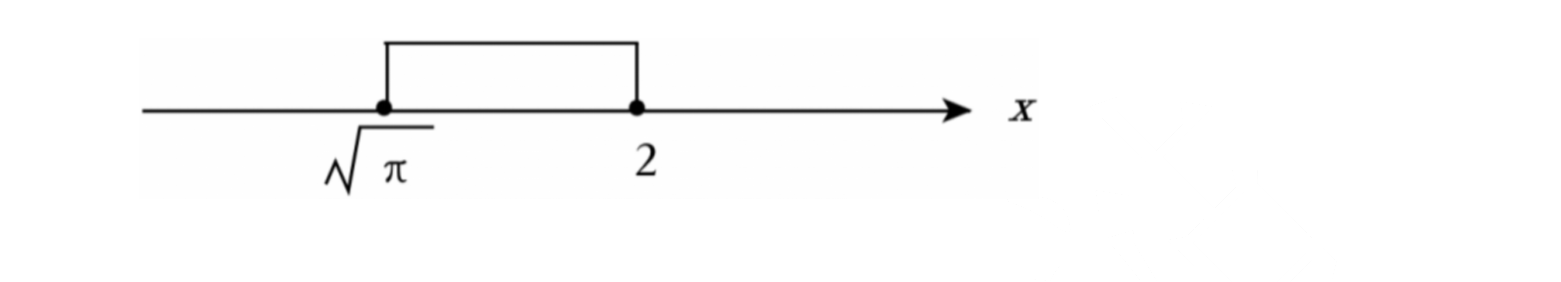
\includegraphics[width=0.72\textwidth]{figures/gao74_q8_numline.png}
\end{center}
\step{所以数形结合得所求集为 $[\sqrt\pi,2]$.}
\solend
\fi

\item 已知集合 $A=\{x\mid(a-1)x^2+3x-3=0,\,x\in\R\}$ 有且仅有一个真子集，则实数 $a=$\blankline[4.4em].

\ifanswer
\solbegin
\step{因为集合 $A=\{x\mid(a-1)x^2+3x-3=0,\,x\in\R\}$ 有且仅有一个真子集，}
\step{所以 $(a-1)x^2+3x-3=0$ 只有一个解，}
\step{所以 $a=1$ 或 $\begin{cases}a\neq1\\ \Delta=3^2-4(a-1)\times(-3)=0\end{cases}$，解得 $a=1$ 或 $a=\dfrac14$.}
\solend
\fi

\item 已知全集 $U=\{(x,y)\mid x,y\in\R\}$，若集合 $A\subseteq U$，且对任意 $(x_1,y_1)\in A$，均存在 $(x_2,y_2)\in A$，使得 $x_1y_2+x_2y_1=0$，则称集合 $A$ 为“对称对点集”. 给出如下集合：

（1）$A=\{(x,y)\mid x,y\in\Z\}$；

（2）$A=\left\{(x,y)\,\middle|\,y=\begin{cases}x+1,&x\geqslant0\\ -x+1,&x<0\end{cases},\ x\in\R,\ x\neq0\right\}$；

（3）$A=\{(x,y)\mid y=x+2,\,x\in\R\}$；

（4）$A=\left\{(x,y)\,\middle|\,y=\dfrac1x,\ x\in\R,\ x\neq0\right\}$.

其中是“对称对点集”的序号为\blankline[4.4em]（写出所有正确的序号）.

\ifanswer
\solbegin
\stepm{(1)}{因为 $0\in\Z$，所以 $(0,0)\in A$.}
\step{对任意 $(x_1,y_1)\in A$，取 $(x_2,y_2)=(0,0)\in A$，}
\step{都有 $x_1\times0+0\times y_1=0$，所以（1）是对称对点集.}
\stepm{(2)}{当 $x_1>0$ 时 $y_1=x_1+1$，取 $x_2=-x_1<0$、$y_2=-x_2+1=x_1+1=y_1$，}
\step{则 $(x_2,y_2)\in A$，且 $x_1y_2+x_2y_1=x_1y_1-x_1y_1=0$；}
\step{当 $x_1<0$ 时同理取 $x_2=-x_1>0$、$y_2=x_2+1=y_1$，}
\step{也有 $(x_2,y_2)\in A$ 且 $x_1y_2+x_2y_1=0$；所以（2）是对称对点集.}
\stepm{(3)}{取 $A$ 中的点 $(-1,1)$. 若存在 $(x_2,y_2)\in A$ 使 $(-1)\cdot y_2+x_2\cdot1=0$，}
\step{则 $y_2=x_2$，但 $A$ 中点的坐标满足 $y=x+2$，两者矛盾，}
\step{所以（3）不是对称对点集.}
\stepm{(4)}{设 $(x_1,y_1)\in A$，则 $x_1\neq0$ 且 $y_1=\dfrac1{x_1}$，}
\step{若存在 $(x_2,y_2)\in A$ 使 $x_1y_2+x_2y_1=0$，}
\step{把 $y_1=\dfrac1{x_1}$、$y_2=\dfrac1{x_2}$（$x_2\neq0$）代入得 $\dfrac{x_1}{x_2}+\dfrac{x_2}{x_1}=0$，即 $x_1^2+x_2^2=0$，}
\step{于是 $x_1=x_2=0$，与 $x_1\neq0$、$x_2\neq0$ 矛盾，所以（4）不是对称对点集.}
\step{故正确的是①②.}
\solend
\fi

\end{enumerate}

\bigsec{二、选择题}

\begin{enumerate}
\setcounter{enumi}{10}

\item “$x>3$”是“$\dfrac{x-1}{x-3}>0$”的\mbox{（\quad）}

\keepwithprev
A. 充分不必要条件\qquad B. 必要不充分条件\qquad C. 充要条件\qquad D. 既不充分也不必要条件

\ifanswer
\solbegin
\step{由 $\dfrac{x-1}{x-3}>0$ 得 $x>3$ 或 $x<1$，故“$x>3$”是“$\dfrac{x-1}{x-3}>0$”的充分不必要条件.}
\step{故选 $A$.}
\solend
\fi

\item 已知 $a,b,c\in\R$，$b>c$，则下列不等式中恒成立的是\mbox{（\quad）}

\keepwithprev
A. $a+b^2>a+c^2$\qquad B. $a^2+b>a^2+c$\qquad C. $ab^2>ac^2$\qquad D. $a^2b>a^2c$

\ifanswer
\solbegin
\step{对于 $A$，取 $b=1,c=-1$，错误；对于 $B$，由不等式的同向可加性得正确；}
\step{对于 $C$，取 $a=1,b=1,c=-2$，错误；对于 $D$，取 $a=0$，错误.}
\step{故选 $B$.}
\solend
\fi

\item 已知关于 $x$ 的不等式 $x^2-2kx+1>0$ 对于一切实数 $x$ 都成立，则实数 $k$ 的取值范围是\mbox{（\quad）}

\keepwithprev
A. $[-1,1]$\qquad B. $(-1,1)$\qquad C. $(-\infty,-1)\cup(1,+\infty)$\qquad D. $\left(-\dfrac12,\dfrac12\right)$

\ifanswer
\solbegin
\step{因为关于 $x$ 的不等式 $x^2-2kx+1>0$ 对于一切实数 $x$ 都成立，}
\step{所以 $\Delta=(-2k)^2-4<0$，即 $4k^2-4<0$，解得 $-1<k<1$，}
\step{所以实数 $k$ 的取值范围是 $(-1,1)$. 故选 $B$.}
\solend
\fi

\item 某种生产设备购买时费用 $100$ 千元，每年的设备管理费 $8$ 千元，这种生产设备的维修费前 $x(x\in\N)$ 年共 $\dfrac{25}{36}x^2+2x$ 千元，问这种生产设备最多使用\mbox{（\quad）}年报废最合算？（即年平均费用最少）

\keepwithprev
A. $13$\qquad B. $10$\qquad C. $15$\qquad D. $12$

\ifanswer
\solbegin
\step{设使用 $x$ 年报废，则总费用 $S(x)=100+8x+\dfrac{25}{36}x^2+2x=\dfrac{25}{36}x^2+10x+100$，}
\step{则年平均费用为 $y=\dfrac{S(x)}x=\dfrac{25x}{36}+\dfrac{100}x+10\geqslant2\sqrt{\dfrac{25x}{36}\cdot\dfrac{100}x}+10=\dfrac{80}3$，}
\step{当且仅当 $\dfrac{25x}{36}=\dfrac{100}x$，即 $x=12$ 时，取等号，}
\step{故当使用 $12$ 年报废，年平均费用最少. 故选 $D$.}
\solend
\fi

\end{enumerate}

\bigsec{三、解答题}

\begin{enumerate}
\setcounter{enumi}{14}

\item （1）设集合 $A=\{x\mid ax-1=0,\,x\in\R\}$，$B=\{x\mid x^2-3x+2=0,\,x\in\R\}$，若 $A\cap B\neq\varnothing$，求实数 $a$ 的取值范围；

（2）已知一元二次方程 $x^2-mx+m+1=0$ 的两个不等实根为 $x_1$、$x_2$，且 $x_1^2+x_2^2=1$，求实数 $m$ 的值.

\ifanswer
\solbegin
\stepm{(1)}{$B=\{x\mid x^2-3x+2=0,\,x\in\R\}=\{1,2\}$，}
\step{①当 $a=0$ 时，方程 $0\cdot x-1=0$ 无解，$A=\varnothing$，$A\cap B=\varnothing$，不符合题意；}
\step{②当 $a\neq0$ 时，$A=\left\{\dfrac1a\right\}$. $A\cap B\neq\varnothing$，}
\step{则 $\dfrac1a\in B$，即 $\dfrac1a=1$ 或 $\dfrac1a=2$，解得 $a=1$ 或 $\dfrac12$；}
\stepm{(2)}{方程 $x^2-mx+m+1=0$ 有两个不等实根，}
\step{则 $\Delta=m^2-4(m+1)>0$，解得 $m>2+2\sqrt2$ 或 $m<2-2\sqrt2$，}
\step{由韦达定理得 $x_1+x_2=m$，$x_1x_2=m+1$，$x_1^2+x_2^2=1$，}
\step{则 $(x_1+x_2)^2-2x_1x_2=m^2-2(m+1)=1$，解得 $m=-1$ 或 $m=3$（舍去），}
\step{综上所述，$m=-1$.}
\solend
\fi

\ansspace

\item 设全集为 $\R$，已知集合 $A=\{x\mid|x-1|\leqslant3,\,x\in\R\}$，

$B=\{x\mid x^2-2mx+(m-3)(m+3)\leqslant0,\,x\in\R\}$.

（1）若 $A\cap B=[0,4]$，求实数 $m$ 的值；

（2）若 $A\cap\overline{B}=A$，求实数 $m$ 的取值范围.

\ifanswer
\solbegin
\stepm{(1)}{$A=\{x\mid|x-1|\leqslant3\}=\{x\mid-2\leqslant x\leqslant4\}$，}
\step{$B=\{x\mid x^2-2mx+(m-3)(m+3)\leqslant0\}=\{x\mid m-3\leqslant x\leqslant m+3\}$，}
\step{若 $A\cap B=[0,4]$，则 $m-3=0$，即 $m=3$；}
\stepm{(2)}{若 $A\cap\overline{B}=A$，则 $A\subseteq\overline{B}$，$\overline{B}=\{x\mid x>m+3\text{ 或 }x<m-3\}$，}
\step{所以 $m+3<-2$ 或 $m-3>4$，解得 $m<-5$ 或 $m>7$，}
\step{实数 $m$ 的取值范围为 $\{m\mid m<-5\text{ 或 }m>7\}$.}
\solend
\fi

\ansspace

\item （1）已知 $a$、$b$ 为正实数，若 $a+b>4$，试用反证法证明：$\dfrac{a}{b+2}$ 和 $\dfrac{b}{a+2}$ 中至少有一个\mbox{大于 $\dfrac12$}；

（2）设 $x$、$y$ 为正实数，$m=\sqrt{2x}+\sqrt{2y}$，$n=\sqrt{x^2+5xy+y^2}$，试比较 $m$、$n$ 的大小，并说明理由.

\ifanswer
\solbegin
\stepm{(1)}{假设 $\dfrac{a}{b+2}\leqslant\dfrac12$ 且 $\dfrac{b}{a+2}\leqslant\dfrac12$，}
\step{又由 $a$、$b$ 为正实数，则有 $2a\leqslant b+2$ 且 $2b\leqslant a+2$，}
\step{两式相加，有 $2a+2b\leqslant a+b+4$，变形得 $a+b\leqslant4$，}
\step{与已知 $a+b>4$ 相矛盾，即假设 $\dfrac{a}{b+2}\leqslant\dfrac12$ 且 $\dfrac{b}{a+2}\leqslant\dfrac12$ 不成立，}
\step{故 $\dfrac{a}{b+2}$ 和 $\dfrac{b}{a+2}$ 中至少有一个\mbox{大于 $\dfrac12$}；}
\stepm{(2)}{$m>n$，理由：$x$、$y$ 为正实数，$m=\sqrt{2x}+\sqrt{2y}$，$n=\sqrt{x^2+5xy+y^2}$，}
\step{则 $m^2=(\sqrt{2x}+\sqrt{2y})^2=2x^2+2y^2+4xy$，$n^2=x^2+y^2+5xy$，}
\step{则有 $m^2-n^2=2x^2+2y^2+4xy-x^2-y^2-5xy=x^2+y^2-xy$}
\step{$=\left(x-\dfrac y2\right)^2+\dfrac{3y^2}4$，}
\step{又 $x$、$y$ 为正实数，则 $m^2-n^2>0$，即 $m^2>n^2$，必有 $m>n$，结论成立.}
\solend
\fi

\ansspace

\item 已知集合 $A=\{a_1,a_2,a_3,\cdots,a_n\}$，$a_i$ 为正整数（$i=1,2,\cdots,n$）.

（1）设 $n=3$，$a_1=1$，$a_2=3$，$a_3=9$，$B=\{a_i+a_j\mid1\leqslant i<j\leqslant3,\,i,j\in\N^*\}$，若互不相同的三个实数 $b_1$、$b_2$、$b_3$，满足 $\{b_i+b_j\mid1\leqslant i<j\leqslant3,\,i,j\in\N^*\}=B$，求有序数组 $(b_1,b_2,b_3)$；

（2）设 $n=4$，$C=\{a_1^2,a_2^2,a_3^2,a_4^2\}$，其中 $a_1<a_2<a_3<a_4$，$A\cap C=\{a_1,a_4\}$，且 $a_1+a_4=10$，$A\cup C$ 中所有元素之和为 $124$，求集合 $A$；

（3）设 $n=2$，有 $7$ 个互不相同的集合 $A$ 分别记为 $A_1$、$A_2$、$A_3$、$\cdots$、$A_7$，且 $A_1\cap A_7=\varnothing$、$A_i\cap A_{i+1}=\varnothing\,(i=1,2,3,\cdots,6)$，记 $D=A_1\cup A_2\cup A_3\cup\cdots\cup A_7$，求 $D$ 中元素个数的最小值.

\ifanswer
\solbegin
\stepm{(1)}{$B=\{a_i+a_j\mid1\leqslant i<j\leqslant3,\,i,j\in\N^*\}=\{1+3,1+9,3+9\}=\{4,10,12\}$，}
\step{由题意，不妨设 $b_1<b_2<b_3$，}
\step{则三个数两两之和为 $\begin{cases}b_1+b_2=4\\ b_1+b_3=10\\ b_2+b_3=12\end{cases}$，解得 $\begin{cases}b_1=1\\ b_2=3\\ b_3=9\end{cases}$，}
\step{所以满足条件的有序数组为 $1$，$3$，$9$ 三个数字的全部排列，}
\step{所以有序数组 $(b_1,b_2,b_3)$ 为 $(1,3,9),(1,9,3),(3,1,9),(3,9,1),(9,1,3),(9,3,1)$；}
\stepm{(2)}{因为 $A\cap C=\{a_1,a_4\}$，所以 $a_1\in C$，$a_4\in C$，}
\step{所以 $a_1$ 是集合 $A$ 中某个正整数的平方，}
\step{又因为 $a_1$ 是最小的正整数，所以只能是 $a_1=1$，此时满足 $1=1^2$.}
\step{又 $a_1+a_4=10$，所以 $a_4=9$，所以 $9$ 也是集合 $A$ 中某个正整数的平方，}
\step{因为 $3^2=9$，所以 $3\in A$，则有 $a_2=3$ 或 $a_3=3$.}
\step{若 $a_3=3$，则 $A=\{1,a_2,3,9\}$，$C=\{1^2,a_2^2,3^2,9^2\}=\{1,a_2^2,9,81\}$，}
\step{因为 $a_1<a_2<a_3<a_4$，且 $a_2$ 为正整数，所以只能是 $a_2=2$，}
\step{故 $A=\{1,2,3,9\}$，$C=\{1,4,9,81\}$，$A\cap C=\{1,9\}$，符合题意，}
\step{则 $A\cup C=\{1,2,3,4,9,81\}$，此时 $1+2+3+4+9+81=100\neq124$，}
\step{故 $a_3=3$ 不符合题意，所以只能 $a_2=3$，}
\step{故 $A=\{1,3,a_3,9\}$，$C=\{1^2,3^2,a_3^2,9^2\}$，此时 $A\cup C=\{1,3,a_3,9,a_3^2,81\}$，}
\step{则有 $1+3+a_3+9+a_3^2+81=124$，}
\step{即 $a_3^2+a_3-30=(a_3+6)(a_3-5)=0$，解得正整数 $a_3=5$，}
\step{此时 $A=\{1,3,5,9\}$，$C=\{1,9,25,81\}$，$A\cup C=\{1,3,5,9,25,81\}$，}
\step{满足 $A\cap C=\{1,9\}$，$A\cup C$ 中所有元素之和为 $1+3+5+9+25+81=124$，}
\step{故 $A=\{1,3,5,9\}$；}
\stepm{(3)}{当 $n=2$ 时，每个集合 $A_i(i=1,2,\cdots,7)$ 均为含有 $2$ 个元素的二元集合，}
\step{设 $D$ 中元素个数为 $m$，}
\step{若 $m\leqslant4$，从 $m$ 个元素中最多能得到 $\dfrac{4\times3}2=6$ 个不同二元集合，不足 $7$ 个，}
\step{故 $m\leqslant4$ 不可能.}
\step{若 $m=5$，则有 $\dfrac{5\times4}2=10$ 个不同二元集合，数量超过 $7$ 个，符合要求.}
\step{因为 $A_i\cap A_{i+1}=\varnothing(i=1,2,3,\cdots,6)$，$A_1\cap A_7=\varnothing$，}
\step{即要求 $7$ 个互不相同的二元集合排成环，}
\step{且相邻（含首尾）集合交集为空集.}
\needvspace{12\baselineskip}
\step{假设 $m=5$，不妨设 $A_1(1,2)$、$A_2(3,4)$、$A_3(1,5)$，则：}
\begin{center}
\renewcommand{\arraystretch}{1.9}
\begin{tabular}{|c|c|c|c|c|}
\hline
$A_4(2,3)$ & $A_5(1,4)$ & $A_6(2,5)$ & $A_7(1,3)$ & 与 $A_1$ 矛盾\\
\hline
 &  & $A_6(3,5)$ & $A_7(2,4)$ & 与 $A_1$ 矛盾\\
\hline
 & $A_5(4,5)$ & $A_6(1,3)$ & $A_7(2,5)$ 或 $A_7(2,4)$ & 与 $A_1$ 矛盾\\
\hline
$A_4(2,4)$ & $A_5(1,3)$ & $A_6(2,5)$ & $A_7(1,4)$ & 与 $A_1$ 矛盾\\
\hline
 &  & $A_6(4,5)$ & $A_7(2,3)$ & 与 $A_1$ 矛盾\\
\hline
 & $A_5(3,5)$ & $A_6(1,4)$ & $A_7(2,3)$ 或 $A_7(2,5)$ & 与 $A_1$ 矛盾\\
\hline
\end{tabular}
\end{center}
\step{故 $m=5$ 不可能.}
\step{综上，$m\geqslant6$，取 $D=\{1,2,3,4,5,6\}$，}
\step{令 $A_1=\{1,2\},A_2=\{3,4\},A_3=\{1,5\},A_4=\{2,4\},A_5=\{3,6\},A_6=\{1,4\}$，}
\step{$A_7=\{5,6\}$，此时 $A_1$、$A_2$、$\cdots$、$A_7$ 是 $7$ 个互不相同的二元集合，}
\step{且 $A_1\cap A_2=\varnothing$，$A_2\cap A_3=\varnothing$，$A_3\cap A_4=\varnothing$，$A_4\cap A_5=\varnothing$，}
\step{$A_5\cap A_6=\varnothing$，$A_6\cap A_7=\varnothing$，$A_7\cap A_1=\varnothing$，满足全部条件，}
\step{故 $D$ 中元素个数的最小值为 $6$.}
\solend
\fi

\ansspace*[7]

\end{enumerate}

\end{document}
"
% 紧凑版：xelatex "\def\iscompact{1}% 高一74_宜川中学_10月月考.tex
%   —— 高一上数学“2026-2027 年宜川中学高一上 10 月月考”（讲评版）
% 试卷版：xelatex 高一74_宜川中学_10月月考.tex
% 答案版：xelatex "\def\isanswer{1}\input{高一74_宜川中学_10月月考.tex}"
% 紧凑版：xelatex "\def\iscompact{1}\input{高一74_宜川中学_10月月考.tex}"
%
% 原始材料：微信公众号“魔都数学加油站”文章，连载“27学年高一74”；
% 原文标题“27学年高一74——2026-2027年上海市宜川中学高一上10月月考”；
% 原文链接：https://mp.weixin.qq.com/s/ymsl2bmkBRY6ZPDiUFCDTA。
% 页面标注发布时间 2026-10-22 21:45（上海）。
% 正文为 9 张 PNG 页（`原图/高一74_宜川中学_10月月考/01..09.png`）：
% 第 1、2、3 页为 4762×6735，其余 6 页为 2560×3620，均按页序读取。
% 9 页全为试卷正文页（卷首标题在第 1 页页顶，卷末第 18 题 (3) 解析止于第 9 页），
% 无封面页、目录页、二维码或宣传页。粉色斜排“魔都数学加油站”为卷面水印，未录入。
%
% 卷首标题：照卷面印作“2026-2027 年宜川中学高一上 10 月月考”（黑体加粗一行）。
% 原卷年份区间用半角连字符，本稿按全稿惯例排 en dash；原卷无副标题。
%
% 篇幅与题号：原卷自第 3 题起编号（第 1、2 题不在本卷内）。填空题 3—10（8 题）、
% 选择题 11—14（4 题）、解答题 15—18（4 题），共 16 题。本稿沿用原节与原题号，
% 只改排为全稿统一的大节样式。
%
% 讲评版：原卷第 3 题只印【答案】（“{(1,1)}”），本稿只给 \ans{}；其余 15 题均印
% 【解析】，用 \solbegin…\solend。四道选择题的作答括号原卷即留空，答案写在解析末句
% “故选 A／B／B／D”，照录在解析内，不另提 \ans{}。
%
% 副标题：原卷未印副标题。本稿按“知识模块”口径标作“集合与常用逻辑用语、不等式”：
% 16 题中集合与常用逻辑用语 7 题（第 3、9、10、15、16、18 题及第 17 题的反证法），
% 不等式 9 题（第 4—8、11—14、17 题），两类均确有分量，故并标。口径同 高一63、高一68—73。
%
% 与原卷的排版差异：
%   ① 原卷每题下直接印【答案】/【解析】，本稿按全稿惯例将答案与解析置于答案版；
%   ② 原卷未印副标题，本稿按“知识模块”口径补出；
%   ③ 原卷填空横线约四个字宽，本稿按全稿惯例统一排 \blankline[4.4em]；
%   ④ 原卷数集记号排斜体 $R$、$Z$、$N$（第 8、9、10、14—18 题），本稿按全稿惯例
%      改用 $\R$、$\Z$、$\N$（同 高一68—73）；第 18 题的正整数集合作 $\N^*$，照录；
%   ⑤ 原卷句末标点多为西文句点，均逐处照录；
%   ⑥ 第 15—18 题的子问原卷印作“（1）…（2）…”，本稿按 高一69—73 成例用行内
%      “（1）（2）（3）”段，解析中的子问标号用 \stepm{(1)}{…}；
%   ⑦ 每道解答题原卷未留作答空白，本稿按全稿惯例加 \ansspace（末题用 \ansspace*）；
%   ⑧ 选择题的作答括号原卷排半角“(    )”，本稿按全稿惯例排 \mbox{（\quad）}；
%      选项行排照原卷——第 11、13 题一行四条，第 12、14 题一行四条；
%   ⑨ 第 9、14、18 题解析中的不等式组／方程组，原卷均排作“{”连接的多行式，
%      本稿按全稿惯例排 cases；
%   ⑩ 第 8 题解析有一幅数轴图：原卷印在【解析】第 2 行之后，题干无“如图”二字。
%      本稿按原卷截图裁取（`figures/gao74_q8_numline.png`，由第 2 页原图裁出、
%      去除粉色水印后转灰度，未放大），放在答案版解析第 2 条之后；
%   ⑪ 第 18 题 (3) 解析中有一张 5 列 6 行的枚举表（原卷无表头、左侧两列留空以表示
%      沿用上格的 $A_4$／$A_5$），本稿照原卷排成同样的空格表，未加表头、未合并单元格。
%
% 原卷笔误/存疑（均照录未改，正文对应处另有 % 注）：
%   ① 第 14 题题干“维修费前 $x(x\in N)$ 年共 $\dfrac{25}{36}x^2+2x$ 千元”中的
%      $N$ 原卷排斜体，按全稿惯例改 $\N$，含义不变；
%   ② 第 18 题 (3) 的枚举表第 1—3 行与第 4—6 行分属“$A_5(1,4)$”“$A_5(1,3)$”两种
%      情形，原卷只在首行重复写 $A_4$、$A_5$，其余留空；本稿照录留空，未补字。
%
% 行数核对：逐题数 \step/\stepm 条数与原卷【解析】印刷行数，15 题逐一相符，
% 合计 104 条 / 104 行（Q4：1；Q5：2；Q6：3；Q7：3；Q8：3；Q9：3；Q10：15；
% Q11：2；Q12：3；Q13：3；Q14：4；Q15：9；Q16：6；Q17：10；Q18：37）。
% 另第 3 题只印【答案】，提 \ans{}，不计入 \step 账。
%
% 插图：第 8 题解析的数轴图，见上⑩；全卷题干无其他配图。
%
\documentclass[a4paper,11pt]{article}
\usepackage{common}

\begin{document}

\examtitlest[3]{2026--2027 年宜川中学高一上 10 月月考}{集合与常用逻辑用语、不等式}

\bigsec{一、填空题}

\begin{enumerate}
\setcounter{enumi}{2}

\item 已知集合 $A=\{(x,y)\mid y=x\}$，集合 $B=\{(x,y)\mid y=2-x\}$，则 $A\cap B=$\blankline[4.4em].

\ifanswer
\ans{$\{(1,1)\}$}
\fi

\item 已知 $a=\log_3 2$，$b=\log_3 8$，则 $3^{2a-b}=$\blankline[4.4em].

\ifanswer
\solbegin
\step{由 $a=\log_3 2$，$b=\log_3 8$，得 $3^a=2$，$3^b=8$，则 $3^{2a-b}=\dfrac{(3^a)^2}{3^b}=\dfrac48=\dfrac12$.}
\solend
\fi

\item 已知等式 $2x^2+3x+5=a(2x+1)(x+1)+c$ 恒成立，则实数 $c=$\blankline[4.4em].

\ifanswer
\solbegin
\step{$2x^2+3x+5=a(2x+1)(x+1)+c=2ax^2+3ax+a+c$，}
\step{则 $\begin{cases}2a=2\\ 3a=3\\ a+c=5\end{cases}$，解得 $c=4$.}
\solend
\fi

\item 已知 $x>0$，$y>0$，且 $\dfrac9x+\dfrac1y=1$，则 $x\cdot y$ 的最小值是\blankline[4.4em].

\ifanswer
\solbegin
\step{$x>0$，$y>0$，且 $1=\dfrac9x+\dfrac1y\geqslant2\sqrt{\dfrac9{xy}}$，}
\step{当且仅当 $x=9y$，即 $y=2$，$x=18$ 时取等号，所以 $xy\geqslant36$，}
\step{则 $x\cdot y$ 的最小值为 $36$.}
\solend
\fi

\item 已知关于 $x$ 的不等式 $x^2+bx+c>0$（$b$、$c$ 为实数）的解集为 $(-\infty,-2)\cup(3,+\infty)$，则不等式 $cx^2-bx+1\leqslant0$ 的解集为\blankline[4.4em].

\ifanswer
\solbegin
\step{由已知得 $-2$、$3$ 为方程 $x^2+bx+c=0$ 的根，所以 $-2+3=-b$，$-2\times3=c$，}
\step{即 $b=-1$，$c=-6$，所以不等式 $cx^2-bx+1\leqslant0$ 可变形为 $-6x^2+x+1\leqslant0$，}
\step{即 $6x^2-x-1\geqslant0$，解得 $x\leqslant-\dfrac13$ 或 $x\geqslant\dfrac12$，所以解集为 $\left(-\infty,-\dfrac13\right]\cup\left[\dfrac12,+\infty\right)$.}
\solend
\fi

\item 设 $x\in\R$，则方程 $|x-2|+|\sqrt\pi-x|=2-\sqrt\pi$ 的解集为\blankline[4.4em].

\ifanswer
\solbegin
\step{因为方程 $|x-2|+|\sqrt\pi-x|=2-\sqrt\pi$ 可化为 $|x-2|+|x-\sqrt\pi|=2-\sqrt\pi$，}
\needvspace{8\baselineskip}
\step{其表示数轴上实数 $x$ 到 $\sqrt\pi$ 与 $2$ 的距离之和等于 $2-\sqrt\pi$，如图：}
\begin{center}
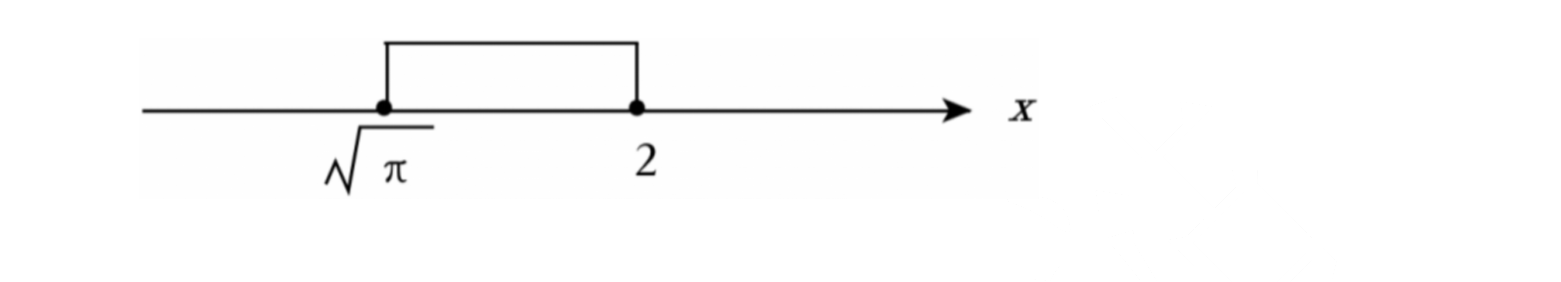
\includegraphics[width=0.72\textwidth]{figures/gao74_q8_numline.png}
\end{center}
\step{所以数形结合得所求集为 $[\sqrt\pi,2]$.}
\solend
\fi

\item 已知集合 $A=\{x\mid(a-1)x^2+3x-3=0,\,x\in\R\}$ 有且仅有一个真子集，则实数 $a=$\blankline[4.4em].

\ifanswer
\solbegin
\step{因为集合 $A=\{x\mid(a-1)x^2+3x-3=0,\,x\in\R\}$ 有且仅有一个真子集，}
\step{所以 $(a-1)x^2+3x-3=0$ 只有一个解，}
\step{所以 $a=1$ 或 $\begin{cases}a\neq1\\ \Delta=3^2-4(a-1)\times(-3)=0\end{cases}$，解得 $a=1$ 或 $a=\dfrac14$.}
\solend
\fi

\item 已知全集 $U=\{(x,y)\mid x,y\in\R\}$，若集合 $A\subseteq U$，且对任意 $(x_1,y_1)\in A$，均存在 $(x_2,y_2)\in A$，使得 $x_1y_2+x_2y_1=0$，则称集合 $A$ 为“对称对点集”. 给出如下集合：

（1）$A=\{(x,y)\mid x,y\in\Z\}$；

（2）$A=\left\{(x,y)\,\middle|\,y=\begin{cases}x+1,&x\geqslant0\\ -x+1,&x<0\end{cases},\ x\in\R,\ x\neq0\right\}$；

（3）$A=\{(x,y)\mid y=x+2,\,x\in\R\}$；

（4）$A=\left\{(x,y)\,\middle|\,y=\dfrac1x,\ x\in\R,\ x\neq0\right\}$.

其中是“对称对点集”的序号为\blankline[4.4em]（写出所有正确的序号）.

\ifanswer
\solbegin
\stepm{(1)}{因为 $0\in\Z$，所以 $(0,0)\in A$.}
\step{对任意 $(x_1,y_1)\in A$，取 $(x_2,y_2)=(0,0)\in A$，}
\step{都有 $x_1\times0+0\times y_1=0$，所以（1）是对称对点集.}
\stepm{(2)}{当 $x_1>0$ 时 $y_1=x_1+1$，取 $x_2=-x_1<0$、$y_2=-x_2+1=x_1+1=y_1$，}
\step{则 $(x_2,y_2)\in A$，且 $x_1y_2+x_2y_1=x_1y_1-x_1y_1=0$；}
\step{当 $x_1<0$ 时同理取 $x_2=-x_1>0$、$y_2=x_2+1=y_1$，}
\step{也有 $(x_2,y_2)\in A$ 且 $x_1y_2+x_2y_1=0$；所以（2）是对称对点集.}
\stepm{(3)}{取 $A$ 中的点 $(-1,1)$. 若存在 $(x_2,y_2)\in A$ 使 $(-1)\cdot y_2+x_2\cdot1=0$，}
\step{则 $y_2=x_2$，但 $A$ 中点的坐标满足 $y=x+2$，两者矛盾，}
\step{所以（3）不是对称对点集.}
\stepm{(4)}{设 $(x_1,y_1)\in A$，则 $x_1\neq0$ 且 $y_1=\dfrac1{x_1}$，}
\step{若存在 $(x_2,y_2)\in A$ 使 $x_1y_2+x_2y_1=0$，}
\step{把 $y_1=\dfrac1{x_1}$、$y_2=\dfrac1{x_2}$（$x_2\neq0$）代入得 $\dfrac{x_1}{x_2}+\dfrac{x_2}{x_1}=0$，即 $x_1^2+x_2^2=0$，}
\step{于是 $x_1=x_2=0$，与 $x_1\neq0$、$x_2\neq0$ 矛盾，所以（4）不是对称对点集.}
\step{故正确的是①②.}
\solend
\fi

\end{enumerate}

\bigsec{二、选择题}

\begin{enumerate}
\setcounter{enumi}{10}

\item “$x>3$”是“$\dfrac{x-1}{x-3}>0$”的\mbox{（\quad）}

\keepwithprev
A. 充分不必要条件\qquad B. 必要不充分条件\qquad C. 充要条件\qquad D. 既不充分也不必要条件

\ifanswer
\solbegin
\step{由 $\dfrac{x-1}{x-3}>0$ 得 $x>3$ 或 $x<1$，故“$x>3$”是“$\dfrac{x-1}{x-3}>0$”的充分不必要条件.}
\step{故选 $A$.}
\solend
\fi

\item 已知 $a,b,c\in\R$，$b>c$，则下列不等式中恒成立的是\mbox{（\quad）}

\keepwithprev
A. $a+b^2>a+c^2$\qquad B. $a^2+b>a^2+c$\qquad C. $ab^2>ac^2$\qquad D. $a^2b>a^2c$

\ifanswer
\solbegin
\step{对于 $A$，取 $b=1,c=-1$，错误；对于 $B$，由不等式的同向可加性得正确；}
\step{对于 $C$，取 $a=1,b=1,c=-2$，错误；对于 $D$，取 $a=0$，错误.}
\step{故选 $B$.}
\solend
\fi

\item 已知关于 $x$ 的不等式 $x^2-2kx+1>0$ 对于一切实数 $x$ 都成立，则实数 $k$ 的取值范围是\mbox{（\quad）}

\keepwithprev
A. $[-1,1]$\qquad B. $(-1,1)$\qquad C. $(-\infty,-1)\cup(1,+\infty)$\qquad D. $\left(-\dfrac12,\dfrac12\right)$

\ifanswer
\solbegin
\step{因为关于 $x$ 的不等式 $x^2-2kx+1>0$ 对于一切实数 $x$ 都成立，}
\step{所以 $\Delta=(-2k)^2-4<0$，即 $4k^2-4<0$，解得 $-1<k<1$，}
\step{所以实数 $k$ 的取值范围是 $(-1,1)$. 故选 $B$.}
\solend
\fi

\item 某种生产设备购买时费用 $100$ 千元，每年的设备管理费 $8$ 千元，这种生产设备的维修费前 $x(x\in\N)$ 年共 $\dfrac{25}{36}x^2+2x$ 千元，问这种生产设备最多使用\mbox{（\quad）}年报废最合算？（即年平均费用最少）

\keepwithprev
A. $13$\qquad B. $10$\qquad C. $15$\qquad D. $12$

\ifanswer
\solbegin
\step{设使用 $x$ 年报废，则总费用 $S(x)=100+8x+\dfrac{25}{36}x^2+2x=\dfrac{25}{36}x^2+10x+100$，}
\step{则年平均费用为 $y=\dfrac{S(x)}x=\dfrac{25x}{36}+\dfrac{100}x+10\geqslant2\sqrt{\dfrac{25x}{36}\cdot\dfrac{100}x}+10=\dfrac{80}3$，}
\step{当且仅当 $\dfrac{25x}{36}=\dfrac{100}x$，即 $x=12$ 时，取等号，}
\step{故当使用 $12$ 年报废，年平均费用最少. 故选 $D$.}
\solend
\fi

\end{enumerate}

\bigsec{三、解答题}

\begin{enumerate}
\setcounter{enumi}{14}

\item （1）设集合 $A=\{x\mid ax-1=0,\,x\in\R\}$，$B=\{x\mid x^2-3x+2=0,\,x\in\R\}$，若 $A\cap B\neq\varnothing$，求实数 $a$ 的取值范围；

（2）已知一元二次方程 $x^2-mx+m+1=0$ 的两个不等实根为 $x_1$、$x_2$，且 $x_1^2+x_2^2=1$，求实数 $m$ 的值.

\ifanswer
\solbegin
\stepm{(1)}{$B=\{x\mid x^2-3x+2=0,\,x\in\R\}=\{1,2\}$，}
\step{①当 $a=0$ 时，方程 $0\cdot x-1=0$ 无解，$A=\varnothing$，$A\cap B=\varnothing$，不符合题意；}
\step{②当 $a\neq0$ 时，$A=\left\{\dfrac1a\right\}$. $A\cap B\neq\varnothing$，}
\step{则 $\dfrac1a\in B$，即 $\dfrac1a=1$ 或 $\dfrac1a=2$，解得 $a=1$ 或 $\dfrac12$；}
\stepm{(2)}{方程 $x^2-mx+m+1=0$ 有两个不等实根，}
\step{则 $\Delta=m^2-4(m+1)>0$，解得 $m>2+2\sqrt2$ 或 $m<2-2\sqrt2$，}
\step{由韦达定理得 $x_1+x_2=m$，$x_1x_2=m+1$，$x_1^2+x_2^2=1$，}
\step{则 $(x_1+x_2)^2-2x_1x_2=m^2-2(m+1)=1$，解得 $m=-1$ 或 $m=3$（舍去），}
\step{综上所述，$m=-1$.}
\solend
\fi

\ansspace

\item 设全集为 $\R$，已知集合 $A=\{x\mid|x-1|\leqslant3,\,x\in\R\}$，

$B=\{x\mid x^2-2mx+(m-3)(m+3)\leqslant0,\,x\in\R\}$.

（1）若 $A\cap B=[0,4]$，求实数 $m$ 的值；

（2）若 $A\cap\overline{B}=A$，求实数 $m$ 的取值范围.

\ifanswer
\solbegin
\stepm{(1)}{$A=\{x\mid|x-1|\leqslant3\}=\{x\mid-2\leqslant x\leqslant4\}$，}
\step{$B=\{x\mid x^2-2mx+(m-3)(m+3)\leqslant0\}=\{x\mid m-3\leqslant x\leqslant m+3\}$，}
\step{若 $A\cap B=[0,4]$，则 $m-3=0$，即 $m=3$；}
\stepm{(2)}{若 $A\cap\overline{B}=A$，则 $A\subseteq\overline{B}$，$\overline{B}=\{x\mid x>m+3\text{ 或 }x<m-3\}$，}
\step{所以 $m+3<-2$ 或 $m-3>4$，解得 $m<-5$ 或 $m>7$，}
\step{实数 $m$ 的取值范围为 $\{m\mid m<-5\text{ 或 }m>7\}$.}
\solend
\fi

\ansspace

\item （1）已知 $a$、$b$ 为正实数，若 $a+b>4$，试用反证法证明：$\dfrac{a}{b+2}$ 和 $\dfrac{b}{a+2}$ 中至少有一个\mbox{大于 $\dfrac12$}；

（2）设 $x$、$y$ 为正实数，$m=\sqrt{2x}+\sqrt{2y}$，$n=\sqrt{x^2+5xy+y^2}$，试比较 $m$、$n$ 的大小，并说明理由.

\ifanswer
\solbegin
\stepm{(1)}{假设 $\dfrac{a}{b+2}\leqslant\dfrac12$ 且 $\dfrac{b}{a+2}\leqslant\dfrac12$，}
\step{又由 $a$、$b$ 为正实数，则有 $2a\leqslant b+2$ 且 $2b\leqslant a+2$，}
\step{两式相加，有 $2a+2b\leqslant a+b+4$，变形得 $a+b\leqslant4$，}
\step{与已知 $a+b>4$ 相矛盾，即假设 $\dfrac{a}{b+2}\leqslant\dfrac12$ 且 $\dfrac{b}{a+2}\leqslant\dfrac12$ 不成立，}
\step{故 $\dfrac{a}{b+2}$ 和 $\dfrac{b}{a+2}$ 中至少有一个\mbox{大于 $\dfrac12$}；}
\stepm{(2)}{$m>n$，理由：$x$、$y$ 为正实数，$m=\sqrt{2x}+\sqrt{2y}$，$n=\sqrt{x^2+5xy+y^2}$，}
\step{则 $m^2=(\sqrt{2x}+\sqrt{2y})^2=2x^2+2y^2+4xy$，$n^2=x^2+y^2+5xy$，}
\step{则有 $m^2-n^2=2x^2+2y^2+4xy-x^2-y^2-5xy=x^2+y^2-xy$}
\step{$=\left(x-\dfrac y2\right)^2+\dfrac{3y^2}4$，}
\step{又 $x$、$y$ 为正实数，则 $m^2-n^2>0$，即 $m^2>n^2$，必有 $m>n$，结论成立.}
\solend
\fi

\ansspace

\item 已知集合 $A=\{a_1,a_2,a_3,\cdots,a_n\}$，$a_i$ 为正整数（$i=1,2,\cdots,n$）.

（1）设 $n=3$，$a_1=1$，$a_2=3$，$a_3=9$，$B=\{a_i+a_j\mid1\leqslant i<j\leqslant3,\,i,j\in\N^*\}$，若互不相同的三个实数 $b_1$、$b_2$、$b_3$，满足 $\{b_i+b_j\mid1\leqslant i<j\leqslant3,\,i,j\in\N^*\}=B$，求有序数组 $(b_1,b_2,b_3)$；

（2）设 $n=4$，$C=\{a_1^2,a_2^2,a_3^2,a_4^2\}$，其中 $a_1<a_2<a_3<a_4$，$A\cap C=\{a_1,a_4\}$，且 $a_1+a_4=10$，$A\cup C$ 中所有元素之和为 $124$，求集合 $A$；

（3）设 $n=2$，有 $7$ 个互不相同的集合 $A$ 分别记为 $A_1$、$A_2$、$A_3$、$\cdots$、$A_7$，且 $A_1\cap A_7=\varnothing$、$A_i\cap A_{i+1}=\varnothing\,(i=1,2,3,\cdots,6)$，记 $D=A_1\cup A_2\cup A_3\cup\cdots\cup A_7$，求 $D$ 中元素个数的最小值.

\ifanswer
\solbegin
\stepm{(1)}{$B=\{a_i+a_j\mid1\leqslant i<j\leqslant3,\,i,j\in\N^*\}=\{1+3,1+9,3+9\}=\{4,10,12\}$，}
\step{由题意，不妨设 $b_1<b_2<b_3$，}
\step{则三个数两两之和为 $\begin{cases}b_1+b_2=4\\ b_1+b_3=10\\ b_2+b_3=12\end{cases}$，解得 $\begin{cases}b_1=1\\ b_2=3\\ b_3=9\end{cases}$，}
\step{所以满足条件的有序数组为 $1$，$3$，$9$ 三个数字的全部排列，}
\step{所以有序数组 $(b_1,b_2,b_3)$ 为 $(1,3,9),(1,9,3),(3,1,9),(3,9,1),(9,1,3),(9,3,1)$；}
\stepm{(2)}{因为 $A\cap C=\{a_1,a_4\}$，所以 $a_1\in C$，$a_4\in C$，}
\step{所以 $a_1$ 是集合 $A$ 中某个正整数的平方，}
\step{又因为 $a_1$ 是最小的正整数，所以只能是 $a_1=1$，此时满足 $1=1^2$.}
\step{又 $a_1+a_4=10$，所以 $a_4=9$，所以 $9$ 也是集合 $A$ 中某个正整数的平方，}
\step{因为 $3^2=9$，所以 $3\in A$，则有 $a_2=3$ 或 $a_3=3$.}
\step{若 $a_3=3$，则 $A=\{1,a_2,3,9\}$，$C=\{1^2,a_2^2,3^2,9^2\}=\{1,a_2^2,9,81\}$，}
\step{因为 $a_1<a_2<a_3<a_4$，且 $a_2$ 为正整数，所以只能是 $a_2=2$，}
\step{故 $A=\{1,2,3,9\}$，$C=\{1,4,9,81\}$，$A\cap C=\{1,9\}$，符合题意，}
\step{则 $A\cup C=\{1,2,3,4,9,81\}$，此时 $1+2+3+4+9+81=100\neq124$，}
\step{故 $a_3=3$ 不符合题意，所以只能 $a_2=3$，}
\step{故 $A=\{1,3,a_3,9\}$，$C=\{1^2,3^2,a_3^2,9^2\}$，此时 $A\cup C=\{1,3,a_3,9,a_3^2,81\}$，}
\step{则有 $1+3+a_3+9+a_3^2+81=124$，}
\step{即 $a_3^2+a_3-30=(a_3+6)(a_3-5)=0$，解得正整数 $a_3=5$，}
\step{此时 $A=\{1,3,5,9\}$，$C=\{1,9,25,81\}$，$A\cup C=\{1,3,5,9,25,81\}$，}
\step{满足 $A\cap C=\{1,9\}$，$A\cup C$ 中所有元素之和为 $1+3+5+9+25+81=124$，}
\step{故 $A=\{1,3,5,9\}$；}
\stepm{(3)}{当 $n=2$ 时，每个集合 $A_i(i=1,2,\cdots,7)$ 均为含有 $2$ 个元素的二元集合，}
\step{设 $D$ 中元素个数为 $m$，}
\step{若 $m\leqslant4$，从 $m$ 个元素中最多能得到 $\dfrac{4\times3}2=6$ 个不同二元集合，不足 $7$ 个，}
\step{故 $m\leqslant4$ 不可能.}
\step{若 $m=5$，则有 $\dfrac{5\times4}2=10$ 个不同二元集合，数量超过 $7$ 个，符合要求.}
\step{因为 $A_i\cap A_{i+1}=\varnothing(i=1,2,3,\cdots,6)$，$A_1\cap A_7=\varnothing$，}
\step{即要求 $7$ 个互不相同的二元集合排成环，}
\step{且相邻（含首尾）集合交集为空集.}
\needvspace{12\baselineskip}
\step{假设 $m=5$，不妨设 $A_1(1,2)$、$A_2(3,4)$、$A_3(1,5)$，则：}
\begin{center}
\renewcommand{\arraystretch}{1.9}
\begin{tabular}{|c|c|c|c|c|}
\hline
$A_4(2,3)$ & $A_5(1,4)$ & $A_6(2,5)$ & $A_7(1,3)$ & 与 $A_1$ 矛盾\\
\hline
 &  & $A_6(3,5)$ & $A_7(2,4)$ & 与 $A_1$ 矛盾\\
\hline
 & $A_5(4,5)$ & $A_6(1,3)$ & $A_7(2,5)$ 或 $A_7(2,4)$ & 与 $A_1$ 矛盾\\
\hline
$A_4(2,4)$ & $A_5(1,3)$ & $A_6(2,5)$ & $A_7(1,4)$ & 与 $A_1$ 矛盾\\
\hline
 &  & $A_6(4,5)$ & $A_7(2,3)$ & 与 $A_1$ 矛盾\\
\hline
 & $A_5(3,5)$ & $A_6(1,4)$ & $A_7(2,3)$ 或 $A_7(2,5)$ & 与 $A_1$ 矛盾\\
\hline
\end{tabular}
\end{center}
\step{故 $m=5$ 不可能.}
\step{综上，$m\geqslant6$，取 $D=\{1,2,3,4,5,6\}$，}
\step{令 $A_1=\{1,2\},A_2=\{3,4\},A_3=\{1,5\},A_4=\{2,4\},A_5=\{3,6\},A_6=\{1,4\}$，}
\step{$A_7=\{5,6\}$，此时 $A_1$、$A_2$、$\cdots$、$A_7$ 是 $7$ 个互不相同的二元集合，}
\step{且 $A_1\cap A_2=\varnothing$，$A_2\cap A_3=\varnothing$，$A_3\cap A_4=\varnothing$，$A_4\cap A_5=\varnothing$，}
\step{$A_5\cap A_6=\varnothing$，$A_6\cap A_7=\varnothing$，$A_7\cap A_1=\varnothing$，满足全部条件，}
\step{故 $D$ 中元素个数的最小值为 $6$.}
\solend
\fi

\ansspace*[7]

\end{enumerate}

\end{document}
"
%
% 原始材料：微信公众号“魔都数学加油站”文章，连载“27学年高一74”；
% 原文标题“27学年高一74——2026-2027年上海市宜川中学高一上10月月考”；
% 原文链接：https://mp.weixin.qq.com/s/ymsl2bmkBRY6ZPDiUFCDTA。
% 页面标注发布时间 2026-10-22 21:45（上海）。
% 正文为 9 张 PNG 页（`原图/高一74_宜川中学_10月月考/01..09.png`）：
% 第 1、2、3 页为 4762×6735，其余 6 页为 2560×3620，均按页序读取。
% 9 页全为试卷正文页（卷首标题在第 1 页页顶，卷末第 18 题 (3) 解析止于第 9 页），
% 无封面页、目录页、二维码或宣传页。粉色斜排“魔都数学加油站”为卷面水印，未录入。
%
% 卷首标题：照卷面印作“2026-2027 年宜川中学高一上 10 月月考”（黑体加粗一行）。
% 原卷年份区间用半角连字符，本稿按全稿惯例排 en dash；原卷无副标题。
%
% 篇幅与题号：原卷自第 3 题起编号（第 1、2 题不在本卷内）。填空题 3—10（8 题）、
% 选择题 11—14（4 题）、解答题 15—18（4 题），共 16 题。本稿沿用原节与原题号，
% 只改排为全稿统一的大节样式。
%
% 讲评版：原卷第 3 题只印【答案】（“{(1,1)}”），本稿只给 \ans{}；其余 15 题均印
% 【解析】，用 \solbegin…\solend。四道选择题的作答括号原卷即留空，答案写在解析末句
% “故选 A／B／B／D”，照录在解析内，不另提 \ans{}。
%
% 副标题：原卷未印副标题。本稿按“知识模块”口径标作“集合与常用逻辑用语、不等式”：
% 16 题中集合与常用逻辑用语 7 题（第 3、9、10、15、16、18 题及第 17 题的反证法），
% 不等式 9 题（第 4—8、11—14、17 题），两类均确有分量，故并标。口径同 高一63、高一68—73。
%
% 与原卷的排版差异：
%   ① 原卷每题下直接印【答案】/【解析】，本稿按全稿惯例将答案与解析置于答案版；
%   ② 原卷未印副标题，本稿按“知识模块”口径补出；
%   ③ 原卷填空横线约四个字宽，本稿按全稿惯例统一排 \blankline[4.4em]；
%   ④ 原卷数集记号排斜体 $R$、$Z$、$N$（第 8、9、10、14—18 题），本稿按全稿惯例
%      改用 $\R$、$\Z$、$\N$（同 高一68—73）；第 18 题的正整数集合作 $\N^*$，照录；
%   ⑤ 原卷句末标点多为西文句点，均逐处照录；
%   ⑥ 第 15—18 题的子问原卷印作“（1）…（2）…”，本稿按 高一69—73 成例用行内
%      “（1）（2）（3）”段，解析中的子问标号用 \stepm{(1)}{…}；
%   ⑦ 每道解答题原卷未留作答空白，本稿按全稿惯例加 \ansspace（末题用 \ansspace*）；
%   ⑧ 选择题的作答括号原卷排半角“(    )”，本稿按全稿惯例排 \mbox{（\quad）}；
%      选项行排照原卷——第 11、13 题一行四条，第 12、14 题一行四条；
%   ⑨ 第 9、14、18 题解析中的不等式组／方程组，原卷均排作“{”连接的多行式，
%      本稿按全稿惯例排 cases；
%   ⑩ 第 8 题解析有一幅数轴图：原卷印在【解析】第 2 行之后，题干无“如图”二字。
%      本稿按原卷截图裁取（`figures/gao74_q8_numline.png`，由第 2 页原图裁出、
%      去除粉色水印后转灰度，未放大），放在答案版解析第 2 条之后；
%   ⑪ 第 18 题 (3) 解析中有一张 5 列 6 行的枚举表（原卷无表头、左侧两列留空以表示
%      沿用上格的 $A_4$／$A_5$），本稿照原卷排成同样的空格表，未加表头、未合并单元格。
%
% 原卷笔误/存疑（均照录未改，正文对应处另有 % 注）：
%   ① 第 14 题题干“维修费前 $x(x\in N)$ 年共 $\dfrac{25}{36}x^2+2x$ 千元”中的
%      $N$ 原卷排斜体，按全稿惯例改 $\N$，含义不变；
%   ② 第 18 题 (3) 的枚举表第 1—3 行与第 4—6 行分属“$A_5(1,4)$”“$A_5(1,3)$”两种
%      情形，原卷只在首行重复写 $A_4$、$A_5$，其余留空；本稿照录留空，未补字。
%
% 行数核对：逐题数 \step/\stepm 条数与原卷【解析】印刷行数，15 题逐一相符，
% 合计 104 条 / 104 行（Q4：1；Q5：2；Q6：3；Q7：3；Q8：3；Q9：3；Q10：15；
% Q11：2；Q12：3；Q13：3；Q14：4；Q15：9；Q16：6；Q17：10；Q18：37）。
% 另第 3 题只印【答案】，提 \ans{}，不计入 \step 账。
%
% 插图：第 8 题解析的数轴图，见上⑩；全卷题干无其他配图。
%
\documentclass[a4paper,11pt]{article}
\usepackage{common}

\begin{document}

\examtitlest[3]{2026--2027 年宜川中学高一上 10 月月考}{集合与常用逻辑用语、不等式}

\bigsec{一、填空题}

\begin{enumerate}
\setcounter{enumi}{2}

\item 已知集合 $A=\{(x,y)\mid y=x\}$，集合 $B=\{(x,y)\mid y=2-x\}$，则 $A\cap B=$\blankline[4.4em].

\ifanswer
\ans{$\{(1,1)\}$}
\fi

\item 已知 $a=\log_3 2$，$b=\log_3 8$，则 $3^{2a-b}=$\blankline[4.4em].

\ifanswer
\solbegin
\step{由 $a=\log_3 2$，$b=\log_3 8$，得 $3^a=2$，$3^b=8$，则 $3^{2a-b}=\dfrac{(3^a)^2}{3^b}=\dfrac48=\dfrac12$.}
\solend
\fi

\item 已知等式 $2x^2+3x+5=a(2x+1)(x+1)+c$ 恒成立，则实数 $c=$\blankline[4.4em].

\ifanswer
\solbegin
\step{$2x^2+3x+5=a(2x+1)(x+1)+c=2ax^2+3ax+a+c$，}
\step{则 $\begin{cases}2a=2\\ 3a=3\\ a+c=5\end{cases}$，解得 $c=4$.}
\solend
\fi

\item 已知 $x>0$，$y>0$，且 $\dfrac9x+\dfrac1y=1$，则 $x\cdot y$ 的最小值是\blankline[4.4em].

\ifanswer
\solbegin
\step{$x>0$，$y>0$，且 $1=\dfrac9x+\dfrac1y\geqslant2\sqrt{\dfrac9{xy}}$，}
\step{当且仅当 $x=9y$，即 $y=2$，$x=18$ 时取等号，所以 $xy\geqslant36$，}
\step{则 $x\cdot y$ 的最小值为 $36$.}
\solend
\fi

\item 已知关于 $x$ 的不等式 $x^2+bx+c>0$（$b$、$c$ 为实数）的解集为 $(-\infty,-2)\cup(3,+\infty)$，则不等式 $cx^2-bx+1\leqslant0$ 的解集为\blankline[4.4em].

\ifanswer
\solbegin
\step{由已知得 $-2$、$3$ 为方程 $x^2+bx+c=0$ 的根，所以 $-2+3=-b$，$-2\times3=c$，}
\step{即 $b=-1$，$c=-6$，所以不等式 $cx^2-bx+1\leqslant0$ 可变形为 $-6x^2+x+1\leqslant0$，}
\step{即 $6x^2-x-1\geqslant0$，解得 $x\leqslant-\dfrac13$ 或 $x\geqslant\dfrac12$，所以解集为 $\left(-\infty,-\dfrac13\right]\cup\left[\dfrac12,+\infty\right)$.}
\solend
\fi

\item 设 $x\in\R$，则方程 $|x-2|+|\sqrt\pi-x|=2-\sqrt\pi$ 的解集为\blankline[4.4em].

\ifanswer
\solbegin
\step{因为方程 $|x-2|+|\sqrt\pi-x|=2-\sqrt\pi$ 可化为 $|x-2|+|x-\sqrt\pi|=2-\sqrt\pi$，}
\needvspace{8\baselineskip}
\step{其表示数轴上实数 $x$ 到 $\sqrt\pi$ 与 $2$ 的距离之和等于 $2-\sqrt\pi$，如图：}
\begin{center}
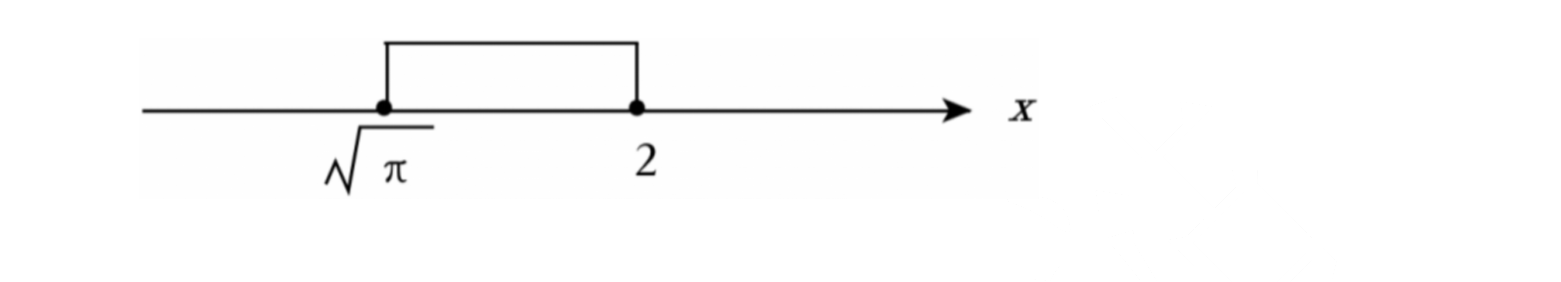
\includegraphics[width=0.72\textwidth]{figures/gao74_q8_numline.png}
\end{center}
\step{所以数形结合得所求集为 $[\sqrt\pi,2]$.}
\solend
\fi

\item 已知集合 $A=\{x\mid(a-1)x^2+3x-3=0,\,x\in\R\}$ 有且仅有一个真子集，则实数 $a=$\blankline[4.4em].

\ifanswer
\solbegin
\step{因为集合 $A=\{x\mid(a-1)x^2+3x-3=0,\,x\in\R\}$ 有且仅有一个真子集，}
\step{所以 $(a-1)x^2+3x-3=0$ 只有一个解，}
\step{所以 $a=1$ 或 $\begin{cases}a\neq1\\ \Delta=3^2-4(a-1)\times(-3)=0\end{cases}$，解得 $a=1$ 或 $a=\dfrac14$.}
\solend
\fi

\item 已知全集 $U=\{(x,y)\mid x,y\in\R\}$，若集合 $A\subseteq U$，且对任意 $(x_1,y_1)\in A$，均存在 $(x_2,y_2)\in A$，使得 $x_1y_2+x_2y_1=0$，则称集合 $A$ 为“对称对点集”. 给出如下集合：

（1）$A=\{(x,y)\mid x,y\in\Z\}$；

（2）$A=\left\{(x,y)\,\middle|\,y=\begin{cases}x+1,&x\geqslant0\\ -x+1,&x<0\end{cases},\ x\in\R,\ x\neq0\right\}$；

（3）$A=\{(x,y)\mid y=x+2,\,x\in\R\}$；

（4）$A=\left\{(x,y)\,\middle|\,y=\dfrac1x,\ x\in\R,\ x\neq0\right\}$.

其中是“对称对点集”的序号为\blankline[4.4em]（写出所有正确的序号）.

\ifanswer
\solbegin
\stepm{(1)}{因为 $0\in\Z$，所以 $(0,0)\in A$.}
\step{对任意 $(x_1,y_1)\in A$，取 $(x_2,y_2)=(0,0)\in A$，}
\step{都有 $x_1\times0+0\times y_1=0$，所以（1）是对称对点集.}
\stepm{(2)}{当 $x_1>0$ 时 $y_1=x_1+1$，取 $x_2=-x_1<0$、$y_2=-x_2+1=x_1+1=y_1$，}
\step{则 $(x_2,y_2)\in A$，且 $x_1y_2+x_2y_1=x_1y_1-x_1y_1=0$；}
\step{当 $x_1<0$ 时同理取 $x_2=-x_1>0$、$y_2=x_2+1=y_1$，}
\step{也有 $(x_2,y_2)\in A$ 且 $x_1y_2+x_2y_1=0$；所以（2）是对称对点集.}
\stepm{(3)}{取 $A$ 中的点 $(-1,1)$. 若存在 $(x_2,y_2)\in A$ 使 $(-1)\cdot y_2+x_2\cdot1=0$，}
\step{则 $y_2=x_2$，但 $A$ 中点的坐标满足 $y=x+2$，两者矛盾，}
\step{所以（3）不是对称对点集.}
\stepm{(4)}{设 $(x_1,y_1)\in A$，则 $x_1\neq0$ 且 $y_1=\dfrac1{x_1}$，}
\step{若存在 $(x_2,y_2)\in A$ 使 $x_1y_2+x_2y_1=0$，}
\step{把 $y_1=\dfrac1{x_1}$、$y_2=\dfrac1{x_2}$（$x_2\neq0$）代入得 $\dfrac{x_1}{x_2}+\dfrac{x_2}{x_1}=0$，即 $x_1^2+x_2^2=0$，}
\step{于是 $x_1=x_2=0$，与 $x_1\neq0$、$x_2\neq0$ 矛盾，所以（4）不是对称对点集.}
\step{故正确的是①②.}
\solend
\fi

\end{enumerate}

\bigsec{二、选择题}

\begin{enumerate}
\setcounter{enumi}{10}

\item “$x>3$”是“$\dfrac{x-1}{x-3}>0$”的\mbox{（\quad）}

\keepwithprev
A. 充分不必要条件\qquad B. 必要不充分条件\qquad C. 充要条件\qquad D. 既不充分也不必要条件

\ifanswer
\solbegin
\step{由 $\dfrac{x-1}{x-3}>0$ 得 $x>3$ 或 $x<1$，故“$x>3$”是“$\dfrac{x-1}{x-3}>0$”的充分不必要条件.}
\step{故选 $A$.}
\solend
\fi

\item 已知 $a,b,c\in\R$，$b>c$，则下列不等式中恒成立的是\mbox{（\quad）}

\keepwithprev
A. $a+b^2>a+c^2$\qquad B. $a^2+b>a^2+c$\qquad C. $ab^2>ac^2$\qquad D. $a^2b>a^2c$

\ifanswer
\solbegin
\step{对于 $A$，取 $b=1,c=-1$，错误；对于 $B$，由不等式的同向可加性得正确；}
\step{对于 $C$，取 $a=1,b=1,c=-2$，错误；对于 $D$，取 $a=0$，错误.}
\step{故选 $B$.}
\solend
\fi

\item 已知关于 $x$ 的不等式 $x^2-2kx+1>0$ 对于一切实数 $x$ 都成立，则实数 $k$ 的取值范围是\mbox{（\quad）}

\keepwithprev
A. $[-1,1]$\qquad B. $(-1,1)$\qquad C. $(-\infty,-1)\cup(1,+\infty)$\qquad D. $\left(-\dfrac12,\dfrac12\right)$

\ifanswer
\solbegin
\step{因为关于 $x$ 的不等式 $x^2-2kx+1>0$ 对于一切实数 $x$ 都成立，}
\step{所以 $\Delta=(-2k)^2-4<0$，即 $4k^2-4<0$，解得 $-1<k<1$，}
\step{所以实数 $k$ 的取值范围是 $(-1,1)$. 故选 $B$.}
\solend
\fi

\item 某种生产设备购买时费用 $100$ 千元，每年的设备管理费 $8$ 千元，这种生产设备的维修费前 $x(x\in\N)$ 年共 $\dfrac{25}{36}x^2+2x$ 千元，问这种生产设备最多使用\mbox{（\quad）}年报废最合算？（即年平均费用最少）

\keepwithprev
A. $13$\qquad B. $10$\qquad C. $15$\qquad D. $12$

\ifanswer
\solbegin
\step{设使用 $x$ 年报废，则总费用 $S(x)=100+8x+\dfrac{25}{36}x^2+2x=\dfrac{25}{36}x^2+10x+100$，}
\step{则年平均费用为 $y=\dfrac{S(x)}x=\dfrac{25x}{36}+\dfrac{100}x+10\geqslant2\sqrt{\dfrac{25x}{36}\cdot\dfrac{100}x}+10=\dfrac{80}3$，}
\step{当且仅当 $\dfrac{25x}{36}=\dfrac{100}x$，即 $x=12$ 时，取等号，}
\step{故当使用 $12$ 年报废，年平均费用最少. 故选 $D$.}
\solend
\fi

\end{enumerate}

\bigsec{三、解答题}

\begin{enumerate}
\setcounter{enumi}{14}

\item （1）设集合 $A=\{x\mid ax-1=0,\,x\in\R\}$，$B=\{x\mid x^2-3x+2=0,\,x\in\R\}$，若 $A\cap B\neq\varnothing$，求实数 $a$ 的取值范围；

（2）已知一元二次方程 $x^2-mx+m+1=0$ 的两个不等实根为 $x_1$、$x_2$，且 $x_1^2+x_2^2=1$，求实数 $m$ 的值.

\ifanswer
\solbegin
\stepm{(1)}{$B=\{x\mid x^2-3x+2=0,\,x\in\R\}=\{1,2\}$，}
\step{①当 $a=0$ 时，方程 $0\cdot x-1=0$ 无解，$A=\varnothing$，$A\cap B=\varnothing$，不符合题意；}
\step{②当 $a\neq0$ 时，$A=\left\{\dfrac1a\right\}$. $A\cap B\neq\varnothing$，}
\step{则 $\dfrac1a\in B$，即 $\dfrac1a=1$ 或 $\dfrac1a=2$，解得 $a=1$ 或 $\dfrac12$；}
\stepm{(2)}{方程 $x^2-mx+m+1=0$ 有两个不等实根，}
\step{则 $\Delta=m^2-4(m+1)>0$，解得 $m>2+2\sqrt2$ 或 $m<2-2\sqrt2$，}
\step{由韦达定理得 $x_1+x_2=m$，$x_1x_2=m+1$，$x_1^2+x_2^2=1$，}
\step{则 $(x_1+x_2)^2-2x_1x_2=m^2-2(m+1)=1$，解得 $m=-1$ 或 $m=3$（舍去），}
\step{综上所述，$m=-1$.}
\solend
\fi

\ansspace

\item 设全集为 $\R$，已知集合 $A=\{x\mid|x-1|\leqslant3,\,x\in\R\}$，

$B=\{x\mid x^2-2mx+(m-3)(m+3)\leqslant0,\,x\in\R\}$.

（1）若 $A\cap B=[0,4]$，求实数 $m$ 的值；

（2）若 $A\cap\overline{B}=A$，求实数 $m$ 的取值范围.

\ifanswer
\solbegin
\stepm{(1)}{$A=\{x\mid|x-1|\leqslant3\}=\{x\mid-2\leqslant x\leqslant4\}$，}
\step{$B=\{x\mid x^2-2mx+(m-3)(m+3)\leqslant0\}=\{x\mid m-3\leqslant x\leqslant m+3\}$，}
\step{若 $A\cap B=[0,4]$，则 $m-3=0$，即 $m=3$；}
\stepm{(2)}{若 $A\cap\overline{B}=A$，则 $A\subseteq\overline{B}$，$\overline{B}=\{x\mid x>m+3\text{ 或 }x<m-3\}$，}
\step{所以 $m+3<-2$ 或 $m-3>4$，解得 $m<-5$ 或 $m>7$，}
\step{实数 $m$ 的取值范围为 $\{m\mid m<-5\text{ 或 }m>7\}$.}
\solend
\fi

\ansspace

\item （1）已知 $a$、$b$ 为正实数，若 $a+b>4$，试用反证法证明：$\dfrac{a}{b+2}$ 和 $\dfrac{b}{a+2}$ 中至少有一个\mbox{大于 $\dfrac12$}；

（2）设 $x$、$y$ 为正实数，$m=\sqrt{2x}+\sqrt{2y}$，$n=\sqrt{x^2+5xy+y^2}$，试比较 $m$、$n$ 的大小，并说明理由.

\ifanswer
\solbegin
\stepm{(1)}{假设 $\dfrac{a}{b+2}\leqslant\dfrac12$ 且 $\dfrac{b}{a+2}\leqslant\dfrac12$，}
\step{又由 $a$、$b$ 为正实数，则有 $2a\leqslant b+2$ 且 $2b\leqslant a+2$，}
\step{两式相加，有 $2a+2b\leqslant a+b+4$，变形得 $a+b\leqslant4$，}
\step{与已知 $a+b>4$ 相矛盾，即假设 $\dfrac{a}{b+2}\leqslant\dfrac12$ 且 $\dfrac{b}{a+2}\leqslant\dfrac12$ 不成立，}
\step{故 $\dfrac{a}{b+2}$ 和 $\dfrac{b}{a+2}$ 中至少有一个\mbox{大于 $\dfrac12$}；}
\stepm{(2)}{$m>n$，理由：$x$、$y$ 为正实数，$m=\sqrt{2x}+\sqrt{2y}$，$n=\sqrt{x^2+5xy+y^2}$，}
\step{则 $m^2=(\sqrt{2x}+\sqrt{2y})^2=2x^2+2y^2+4xy$，$n^2=x^2+y^2+5xy$，}
\step{则有 $m^2-n^2=2x^2+2y^2+4xy-x^2-y^2-5xy=x^2+y^2-xy$}
\step{$=\left(x-\dfrac y2\right)^2+\dfrac{3y^2}4$，}
\step{又 $x$、$y$ 为正实数，则 $m^2-n^2>0$，即 $m^2>n^2$，必有 $m>n$，结论成立.}
\solend
\fi

\ansspace

\item 已知集合 $A=\{a_1,a_2,a_3,\cdots,a_n\}$，$a_i$ 为正整数（$i=1,2,\cdots,n$）.

（1）设 $n=3$，$a_1=1$，$a_2=3$，$a_3=9$，$B=\{a_i+a_j\mid1\leqslant i<j\leqslant3,\,i,j\in\N^*\}$，若互不相同的三个实数 $b_1$、$b_2$、$b_3$，满足 $\{b_i+b_j\mid1\leqslant i<j\leqslant3,\,i,j\in\N^*\}=B$，求有序数组 $(b_1,b_2,b_3)$；

（2）设 $n=4$，$C=\{a_1^2,a_2^2,a_3^2,a_4^2\}$，其中 $a_1<a_2<a_3<a_4$，$A\cap C=\{a_1,a_4\}$，且 $a_1+a_4=10$，$A\cup C$ 中所有元素之和为 $124$，求集合 $A$；

（3）设 $n=2$，有 $7$ 个互不相同的集合 $A$ 分别记为 $A_1$、$A_2$、$A_3$、$\cdots$、$A_7$，且 $A_1\cap A_7=\varnothing$、$A_i\cap A_{i+1}=\varnothing\,(i=1,2,3,\cdots,6)$，记 $D=A_1\cup A_2\cup A_3\cup\cdots\cup A_7$，求 $D$ 中元素个数的最小值.

\ifanswer
\solbegin
\stepm{(1)}{$B=\{a_i+a_j\mid1\leqslant i<j\leqslant3,\,i,j\in\N^*\}=\{1+3,1+9,3+9\}=\{4,10,12\}$，}
\step{由题意，不妨设 $b_1<b_2<b_3$，}
\step{则三个数两两之和为 $\begin{cases}b_1+b_2=4\\ b_1+b_3=10\\ b_2+b_3=12\end{cases}$，解得 $\begin{cases}b_1=1\\ b_2=3\\ b_3=9\end{cases}$，}
\step{所以满足条件的有序数组为 $1$，$3$，$9$ 三个数字的全部排列，}
\step{所以有序数组 $(b_1,b_2,b_3)$ 为 $(1,3,9),(1,9,3),(3,1,9),(3,9,1),(9,1,3),(9,3,1)$；}
\stepm{(2)}{因为 $A\cap C=\{a_1,a_4\}$，所以 $a_1\in C$，$a_4\in C$，}
\step{所以 $a_1$ 是集合 $A$ 中某个正整数的平方，}
\step{又因为 $a_1$ 是最小的正整数，所以只能是 $a_1=1$，此时满足 $1=1^2$.}
\step{又 $a_1+a_4=10$，所以 $a_4=9$，所以 $9$ 也是集合 $A$ 中某个正整数的平方，}
\step{因为 $3^2=9$，所以 $3\in A$，则有 $a_2=3$ 或 $a_3=3$.}
\step{若 $a_3=3$，则 $A=\{1,a_2,3,9\}$，$C=\{1^2,a_2^2,3^2,9^2\}=\{1,a_2^2,9,81\}$，}
\step{因为 $a_1<a_2<a_3<a_4$，且 $a_2$ 为正整数，所以只能是 $a_2=2$，}
\step{故 $A=\{1,2,3,9\}$，$C=\{1,4,9,81\}$，$A\cap C=\{1,9\}$，符合题意，}
\step{则 $A\cup C=\{1,2,3,4,9,81\}$，此时 $1+2+3+4+9+81=100\neq124$，}
\step{故 $a_3=3$ 不符合题意，所以只能 $a_2=3$，}
\step{故 $A=\{1,3,a_3,9\}$，$C=\{1^2,3^2,a_3^2,9^2\}$，此时 $A\cup C=\{1,3,a_3,9,a_3^2,81\}$，}
\step{则有 $1+3+a_3+9+a_3^2+81=124$，}
\step{即 $a_3^2+a_3-30=(a_3+6)(a_3-5)=0$，解得正整数 $a_3=5$，}
\step{此时 $A=\{1,3,5,9\}$，$C=\{1,9,25,81\}$，$A\cup C=\{1,3,5,9,25,81\}$，}
\step{满足 $A\cap C=\{1,9\}$，$A\cup C$ 中所有元素之和为 $1+3+5+9+25+81=124$，}
\step{故 $A=\{1,3,5,9\}$；}
\stepm{(3)}{当 $n=2$ 时，每个集合 $A_i(i=1,2,\cdots,7)$ 均为含有 $2$ 个元素的二元集合，}
\step{设 $D$ 中元素个数为 $m$，}
\step{若 $m\leqslant4$，从 $m$ 个元素中最多能得到 $\dfrac{4\times3}2=6$ 个不同二元集合，不足 $7$ 个，}
\step{故 $m\leqslant4$ 不可能.}
\step{若 $m=5$，则有 $\dfrac{5\times4}2=10$ 个不同二元集合，数量超过 $7$ 个，符合要求.}
\step{因为 $A_i\cap A_{i+1}=\varnothing(i=1,2,3,\cdots,6)$，$A_1\cap A_7=\varnothing$，}
\step{即要求 $7$ 个互不相同的二元集合排成环，}
\step{且相邻（含首尾）集合交集为空集.}
\needvspace{12\baselineskip}
\step{假设 $m=5$，不妨设 $A_1(1,2)$、$A_2(3,4)$、$A_3(1,5)$，则：}
\begin{center}
\renewcommand{\arraystretch}{1.9}
\begin{tabular}{|c|c|c|c|c|}
\hline
$A_4(2,3)$ & $A_5(1,4)$ & $A_6(2,5)$ & $A_7(1,3)$ & 与 $A_1$ 矛盾\\
\hline
 &  & $A_6(3,5)$ & $A_7(2,4)$ & 与 $A_1$ 矛盾\\
\hline
 & $A_5(4,5)$ & $A_6(1,3)$ & $A_7(2,5)$ 或 $A_7(2,4)$ & 与 $A_1$ 矛盾\\
\hline
$A_4(2,4)$ & $A_5(1,3)$ & $A_6(2,5)$ & $A_7(1,4)$ & 与 $A_1$ 矛盾\\
\hline
 &  & $A_6(4,5)$ & $A_7(2,3)$ & 与 $A_1$ 矛盾\\
\hline
 & $A_5(3,5)$ & $A_6(1,4)$ & $A_7(2,3)$ 或 $A_7(2,5)$ & 与 $A_1$ 矛盾\\
\hline
\end{tabular}
\end{center}
\step{故 $m=5$ 不可能.}
\step{综上，$m\geqslant6$，取 $D=\{1,2,3,4,5,6\}$，}
\step{令 $A_1=\{1,2\},A_2=\{3,4\},A_3=\{1,5\},A_4=\{2,4\},A_5=\{3,6\},A_6=\{1,4\}$，}
\step{$A_7=\{5,6\}$，此时 $A_1$、$A_2$、$\cdots$、$A_7$ 是 $7$ 个互不相同的二元集合，}
\step{且 $A_1\cap A_2=\varnothing$，$A_2\cap A_3=\varnothing$，$A_3\cap A_4=\varnothing$，$A_4\cap A_5=\varnothing$，}
\step{$A_5\cap A_6=\varnothing$，$A_6\cap A_7=\varnothing$，$A_7\cap A_1=\varnothing$，满足全部条件，}
\step{故 $D$ 中元素个数的最小值为 $6$.}
\solend
\fi

\ansspace*[7]

\end{enumerate}

\end{document}
"
% 紧凑版：xelatex "\def\iscompact{1}% 高一74_宜川中学_10月月考.tex
%   —— 高一上数学“2026-2027 年宜川中学高一上 10 月月考”（讲评版）
% 试卷版：xelatex 高一74_宜川中学_10月月考.tex
% 答案版：xelatex "\def\isanswer{1}% 高一74_宜川中学_10月月考.tex
%   —— 高一上数学“2026-2027 年宜川中学高一上 10 月月考”（讲评版）
% 试卷版：xelatex 高一74_宜川中学_10月月考.tex
% 答案版：xelatex "\def\isanswer{1}\input{高一74_宜川中学_10月月考.tex}"
% 紧凑版：xelatex "\def\iscompact{1}\input{高一74_宜川中学_10月月考.tex}"
%
% 原始材料：微信公众号“魔都数学加油站”文章，连载“27学年高一74”；
% 原文标题“27学年高一74——2026-2027年上海市宜川中学高一上10月月考”；
% 原文链接：https://mp.weixin.qq.com/s/ymsl2bmkBRY6ZPDiUFCDTA。
% 页面标注发布时间 2026-10-22 21:45（上海）。
% 正文为 9 张 PNG 页（`原图/高一74_宜川中学_10月月考/01..09.png`）：
% 第 1、2、3 页为 4762×6735，其余 6 页为 2560×3620，均按页序读取。
% 9 页全为试卷正文页（卷首标题在第 1 页页顶，卷末第 18 题 (3) 解析止于第 9 页），
% 无封面页、目录页、二维码或宣传页。粉色斜排“魔都数学加油站”为卷面水印，未录入。
%
% 卷首标题：照卷面印作“2026-2027 年宜川中学高一上 10 月月考”（黑体加粗一行）。
% 原卷年份区间用半角连字符，本稿按全稿惯例排 en dash；原卷无副标题。
%
% 篇幅与题号：原卷自第 3 题起编号（第 1、2 题不在本卷内）。填空题 3—10（8 题）、
% 选择题 11—14（4 题）、解答题 15—18（4 题），共 16 题。本稿沿用原节与原题号，
% 只改排为全稿统一的大节样式。
%
% 讲评版：原卷第 3 题只印【答案】（“{(1,1)}”），本稿只给 \ans{}；其余 15 题均印
% 【解析】，用 \solbegin…\solend。四道选择题的作答括号原卷即留空，答案写在解析末句
% “故选 A／B／B／D”，照录在解析内，不另提 \ans{}。
%
% 副标题：原卷未印副标题。本稿按“知识模块”口径标作“集合与常用逻辑用语、不等式”：
% 16 题中集合与常用逻辑用语 7 题（第 3、9、10、15、16、18 题及第 17 题的反证法），
% 不等式 9 题（第 4—8、11—14、17 题），两类均确有分量，故并标。口径同 高一63、高一68—73。
%
% 与原卷的排版差异：
%   ① 原卷每题下直接印【答案】/【解析】，本稿按全稿惯例将答案与解析置于答案版；
%   ② 原卷未印副标题，本稿按“知识模块”口径补出；
%   ③ 原卷填空横线约四个字宽，本稿按全稿惯例统一排 \blankline[4.4em]；
%   ④ 原卷数集记号排斜体 $R$、$Z$、$N$（第 8、9、10、14—18 题），本稿按全稿惯例
%      改用 $\R$、$\Z$、$\N$（同 高一68—73）；第 18 题的正整数集合作 $\N^*$，照录；
%   ⑤ 原卷句末标点多为西文句点，均逐处照录；
%   ⑥ 第 15—18 题的子问原卷印作“（1）…（2）…”，本稿按 高一69—73 成例用行内
%      “（1）（2）（3）”段，解析中的子问标号用 \stepm{(1)}{…}；
%   ⑦ 每道解答题原卷未留作答空白，本稿按全稿惯例加 \ansspace（末题用 \ansspace*）；
%   ⑧ 选择题的作答括号原卷排半角“(    )”，本稿按全稿惯例排 \mbox{（\quad）}；
%      选项行排照原卷——第 11、13 题一行四条，第 12、14 题一行四条；
%   ⑨ 第 9、14、18 题解析中的不等式组／方程组，原卷均排作“{”连接的多行式，
%      本稿按全稿惯例排 cases；
%   ⑩ 第 8 题解析有一幅数轴图：原卷印在【解析】第 2 行之后，题干无“如图”二字。
%      本稿按原卷截图裁取（`figures/gao74_q8_numline.png`，由第 2 页原图裁出、
%      去除粉色水印后转灰度，未放大），放在答案版解析第 2 条之后；
%   ⑪ 第 18 题 (3) 解析中有一张 5 列 6 行的枚举表（原卷无表头、左侧两列留空以表示
%      沿用上格的 $A_4$／$A_5$），本稿照原卷排成同样的空格表，未加表头、未合并单元格。
%
% 原卷笔误/存疑（均照录未改，正文对应处另有 % 注）：
%   ① 第 14 题题干“维修费前 $x(x\in N)$ 年共 $\dfrac{25}{36}x^2+2x$ 千元”中的
%      $N$ 原卷排斜体，按全稿惯例改 $\N$，含义不变；
%   ② 第 18 题 (3) 的枚举表第 1—3 行与第 4—6 行分属“$A_5(1,4)$”“$A_5(1,3)$”两种
%      情形，原卷只在首行重复写 $A_4$、$A_5$，其余留空；本稿照录留空，未补字。
%
% 行数核对：逐题数 \step/\stepm 条数与原卷【解析】印刷行数，15 题逐一相符，
% 合计 104 条 / 104 行（Q4：1；Q5：2；Q6：3；Q7：3；Q8：3；Q9：3；Q10：15；
% Q11：2；Q12：3；Q13：3；Q14：4；Q15：9；Q16：6；Q17：10；Q18：37）。
% 另第 3 题只印【答案】，提 \ans{}，不计入 \step 账。
%
% 插图：第 8 题解析的数轴图，见上⑩；全卷题干无其他配图。
%
\documentclass[a4paper,11pt]{article}
\usepackage{common}

\begin{document}

\examtitlest[3]{2026--2027 年宜川中学高一上 10 月月考}{集合与常用逻辑用语、不等式}

\bigsec{一、填空题}

\begin{enumerate}
\setcounter{enumi}{2}

\item 已知集合 $A=\{(x,y)\mid y=x\}$，集合 $B=\{(x,y)\mid y=2-x\}$，则 $A\cap B=$\blankline[4.4em].

\ifanswer
\ans{$\{(1,1)\}$}
\fi

\item 已知 $a=\log_3 2$，$b=\log_3 8$，则 $3^{2a-b}=$\blankline[4.4em].

\ifanswer
\solbegin
\step{由 $a=\log_3 2$，$b=\log_3 8$，得 $3^a=2$，$3^b=8$，则 $3^{2a-b}=\dfrac{(3^a)^2}{3^b}=\dfrac48=\dfrac12$.}
\solend
\fi

\item 已知等式 $2x^2+3x+5=a(2x+1)(x+1)+c$ 恒成立，则实数 $c=$\blankline[4.4em].

\ifanswer
\solbegin
\step{$2x^2+3x+5=a(2x+1)(x+1)+c=2ax^2+3ax+a+c$，}
\step{则 $\begin{cases}2a=2\\ 3a=3\\ a+c=5\end{cases}$，解得 $c=4$.}
\solend
\fi

\item 已知 $x>0$，$y>0$，且 $\dfrac9x+\dfrac1y=1$，则 $x\cdot y$ 的最小值是\blankline[4.4em].

\ifanswer
\solbegin
\step{$x>0$，$y>0$，且 $1=\dfrac9x+\dfrac1y\geqslant2\sqrt{\dfrac9{xy}}$，}
\step{当且仅当 $x=9y$，即 $y=2$，$x=18$ 时取等号，所以 $xy\geqslant36$，}
\step{则 $x\cdot y$ 的最小值为 $36$.}
\solend
\fi

\item 已知关于 $x$ 的不等式 $x^2+bx+c>0$（$b$、$c$ 为实数）的解集为 $(-\infty,-2)\cup(3,+\infty)$，则不等式 $cx^2-bx+1\leqslant0$ 的解集为\blankline[4.4em].

\ifanswer
\solbegin
\step{由已知得 $-2$、$3$ 为方程 $x^2+bx+c=0$ 的根，所以 $-2+3=-b$，$-2\times3=c$，}
\step{即 $b=-1$，$c=-6$，所以不等式 $cx^2-bx+1\leqslant0$ 可变形为 $-6x^2+x+1\leqslant0$，}
\step{即 $6x^2-x-1\geqslant0$，解得 $x\leqslant-\dfrac13$ 或 $x\geqslant\dfrac12$，所以解集为 $\left(-\infty,-\dfrac13\right]\cup\left[\dfrac12,+\infty\right)$.}
\solend
\fi

\item 设 $x\in\R$，则方程 $|x-2|+|\sqrt\pi-x|=2-\sqrt\pi$ 的解集为\blankline[4.4em].

\ifanswer
\solbegin
\step{因为方程 $|x-2|+|\sqrt\pi-x|=2-\sqrt\pi$ 可化为 $|x-2|+|x-\sqrt\pi|=2-\sqrt\pi$，}
\needvspace{8\baselineskip}
\step{其表示数轴上实数 $x$ 到 $\sqrt\pi$ 与 $2$ 的距离之和等于 $2-\sqrt\pi$，如图：}
\begin{center}
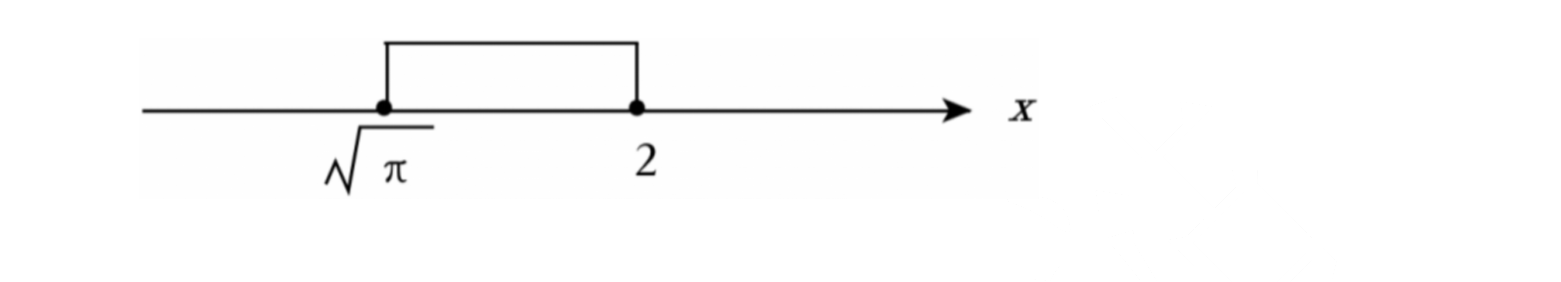
\includegraphics[width=0.72\textwidth]{figures/gao74_q8_numline.png}
\end{center}
\step{所以数形结合得所求集为 $[\sqrt\pi,2]$.}
\solend
\fi

\item 已知集合 $A=\{x\mid(a-1)x^2+3x-3=0,\,x\in\R\}$ 有且仅有一个真子集，则实数 $a=$\blankline[4.4em].

\ifanswer
\solbegin
\step{因为集合 $A=\{x\mid(a-1)x^2+3x-3=0,\,x\in\R\}$ 有且仅有一个真子集，}
\step{所以 $(a-1)x^2+3x-3=0$ 只有一个解，}
\step{所以 $a=1$ 或 $\begin{cases}a\neq1\\ \Delta=3^2-4(a-1)\times(-3)=0\end{cases}$，解得 $a=1$ 或 $a=\dfrac14$.}
\solend
\fi

\item 已知全集 $U=\{(x,y)\mid x,y\in\R\}$，若集合 $A\subseteq U$，且对任意 $(x_1,y_1)\in A$，均存在 $(x_2,y_2)\in A$，使得 $x_1y_2+x_2y_1=0$，则称集合 $A$ 为“对称对点集”. 给出如下集合：

（1）$A=\{(x,y)\mid x,y\in\Z\}$；

（2）$A=\left\{(x,y)\,\middle|\,y=\begin{cases}x+1,&x\geqslant0\\ -x+1,&x<0\end{cases},\ x\in\R,\ x\neq0\right\}$；

（3）$A=\{(x,y)\mid y=x+2,\,x\in\R\}$；

（4）$A=\left\{(x,y)\,\middle|\,y=\dfrac1x,\ x\in\R,\ x\neq0\right\}$.

其中是“对称对点集”的序号为\blankline[4.4em]（写出所有正确的序号）.

\ifanswer
\solbegin
\stepm{(1)}{因为 $0\in\Z$，所以 $(0,0)\in A$.}
\step{对任意 $(x_1,y_1)\in A$，取 $(x_2,y_2)=(0,0)\in A$，}
\step{都有 $x_1\times0+0\times y_1=0$，所以（1）是对称对点集.}
\stepm{(2)}{当 $x_1>0$ 时 $y_1=x_1+1$，取 $x_2=-x_1<0$、$y_2=-x_2+1=x_1+1=y_1$，}
\step{则 $(x_2,y_2)\in A$，且 $x_1y_2+x_2y_1=x_1y_1-x_1y_1=0$；}
\step{当 $x_1<0$ 时同理取 $x_2=-x_1>0$、$y_2=x_2+1=y_1$，}
\step{也有 $(x_2,y_2)\in A$ 且 $x_1y_2+x_2y_1=0$；所以（2）是对称对点集.}
\stepm{(3)}{取 $A$ 中的点 $(-1,1)$. 若存在 $(x_2,y_2)\in A$ 使 $(-1)\cdot y_2+x_2\cdot1=0$，}
\step{则 $y_2=x_2$，但 $A$ 中点的坐标满足 $y=x+2$，两者矛盾，}
\step{所以（3）不是对称对点集.}
\stepm{(4)}{设 $(x_1,y_1)\in A$，则 $x_1\neq0$ 且 $y_1=\dfrac1{x_1}$，}
\step{若存在 $(x_2,y_2)\in A$ 使 $x_1y_2+x_2y_1=0$，}
\step{把 $y_1=\dfrac1{x_1}$、$y_2=\dfrac1{x_2}$（$x_2\neq0$）代入得 $\dfrac{x_1}{x_2}+\dfrac{x_2}{x_1}=0$，即 $x_1^2+x_2^2=0$，}
\step{于是 $x_1=x_2=0$，与 $x_1\neq0$、$x_2\neq0$ 矛盾，所以（4）不是对称对点集.}
\step{故正确的是①②.}
\solend
\fi

\end{enumerate}

\bigsec{二、选择题}

\begin{enumerate}
\setcounter{enumi}{10}

\item “$x>3$”是“$\dfrac{x-1}{x-3}>0$”的\mbox{（\quad）}

\keepwithprev
A. 充分不必要条件\qquad B. 必要不充分条件\qquad C. 充要条件\qquad D. 既不充分也不必要条件

\ifanswer
\solbegin
\step{由 $\dfrac{x-1}{x-3}>0$ 得 $x>3$ 或 $x<1$，故“$x>3$”是“$\dfrac{x-1}{x-3}>0$”的充分不必要条件.}
\step{故选 $A$.}
\solend
\fi

\item 已知 $a,b,c\in\R$，$b>c$，则下列不等式中恒成立的是\mbox{（\quad）}

\keepwithprev
A. $a+b^2>a+c^2$\qquad B. $a^2+b>a^2+c$\qquad C. $ab^2>ac^2$\qquad D. $a^2b>a^2c$

\ifanswer
\solbegin
\step{对于 $A$，取 $b=1,c=-1$，错误；对于 $B$，由不等式的同向可加性得正确；}
\step{对于 $C$，取 $a=1,b=1,c=-2$，错误；对于 $D$，取 $a=0$，错误.}
\step{故选 $B$.}
\solend
\fi

\item 已知关于 $x$ 的不等式 $x^2-2kx+1>0$ 对于一切实数 $x$ 都成立，则实数 $k$ 的取值范围是\mbox{（\quad）}

\keepwithprev
A. $[-1,1]$\qquad B. $(-1,1)$\qquad C. $(-\infty,-1)\cup(1,+\infty)$\qquad D. $\left(-\dfrac12,\dfrac12\right)$

\ifanswer
\solbegin
\step{因为关于 $x$ 的不等式 $x^2-2kx+1>0$ 对于一切实数 $x$ 都成立，}
\step{所以 $\Delta=(-2k)^2-4<0$，即 $4k^2-4<0$，解得 $-1<k<1$，}
\step{所以实数 $k$ 的取值范围是 $(-1,1)$. 故选 $B$.}
\solend
\fi

\item 某种生产设备购买时费用 $100$ 千元，每年的设备管理费 $8$ 千元，这种生产设备的维修费前 $x(x\in\N)$ 年共 $\dfrac{25}{36}x^2+2x$ 千元，问这种生产设备最多使用\mbox{（\quad）}年报废最合算？（即年平均费用最少）

\keepwithprev
A. $13$\qquad B. $10$\qquad C. $15$\qquad D. $12$

\ifanswer
\solbegin
\step{设使用 $x$ 年报废，则总费用 $S(x)=100+8x+\dfrac{25}{36}x^2+2x=\dfrac{25}{36}x^2+10x+100$，}
\step{则年平均费用为 $y=\dfrac{S(x)}x=\dfrac{25x}{36}+\dfrac{100}x+10\geqslant2\sqrt{\dfrac{25x}{36}\cdot\dfrac{100}x}+10=\dfrac{80}3$，}
\step{当且仅当 $\dfrac{25x}{36}=\dfrac{100}x$，即 $x=12$ 时，取等号，}
\step{故当使用 $12$ 年报废，年平均费用最少. 故选 $D$.}
\solend
\fi

\end{enumerate}

\bigsec{三、解答题}

\begin{enumerate}
\setcounter{enumi}{14}

\item （1）设集合 $A=\{x\mid ax-1=0,\,x\in\R\}$，$B=\{x\mid x^2-3x+2=0,\,x\in\R\}$，若 $A\cap B\neq\varnothing$，求实数 $a$ 的取值范围；

（2）已知一元二次方程 $x^2-mx+m+1=0$ 的两个不等实根为 $x_1$、$x_2$，且 $x_1^2+x_2^2=1$，求实数 $m$ 的值.

\ifanswer
\solbegin
\stepm{(1)}{$B=\{x\mid x^2-3x+2=0,\,x\in\R\}=\{1,2\}$，}
\step{①当 $a=0$ 时，方程 $0\cdot x-1=0$ 无解，$A=\varnothing$，$A\cap B=\varnothing$，不符合题意；}
\step{②当 $a\neq0$ 时，$A=\left\{\dfrac1a\right\}$. $A\cap B\neq\varnothing$，}
\step{则 $\dfrac1a\in B$，即 $\dfrac1a=1$ 或 $\dfrac1a=2$，解得 $a=1$ 或 $\dfrac12$；}
\stepm{(2)}{方程 $x^2-mx+m+1=0$ 有两个不等实根，}
\step{则 $\Delta=m^2-4(m+1)>0$，解得 $m>2+2\sqrt2$ 或 $m<2-2\sqrt2$，}
\step{由韦达定理得 $x_1+x_2=m$，$x_1x_2=m+1$，$x_1^2+x_2^2=1$，}
\step{则 $(x_1+x_2)^2-2x_1x_2=m^2-2(m+1)=1$，解得 $m=-1$ 或 $m=3$（舍去），}
\step{综上所述，$m=-1$.}
\solend
\fi

\ansspace

\item 设全集为 $\R$，已知集合 $A=\{x\mid|x-1|\leqslant3,\,x\in\R\}$，

$B=\{x\mid x^2-2mx+(m-3)(m+3)\leqslant0,\,x\in\R\}$.

（1）若 $A\cap B=[0,4]$，求实数 $m$ 的值；

（2）若 $A\cap\overline{B}=A$，求实数 $m$ 的取值范围.

\ifanswer
\solbegin
\stepm{(1)}{$A=\{x\mid|x-1|\leqslant3\}=\{x\mid-2\leqslant x\leqslant4\}$，}
\step{$B=\{x\mid x^2-2mx+(m-3)(m+3)\leqslant0\}=\{x\mid m-3\leqslant x\leqslant m+3\}$，}
\step{若 $A\cap B=[0,4]$，则 $m-3=0$，即 $m=3$；}
\stepm{(2)}{若 $A\cap\overline{B}=A$，则 $A\subseteq\overline{B}$，$\overline{B}=\{x\mid x>m+3\text{ 或 }x<m-3\}$，}
\step{所以 $m+3<-2$ 或 $m-3>4$，解得 $m<-5$ 或 $m>7$，}
\step{实数 $m$ 的取值范围为 $\{m\mid m<-5\text{ 或 }m>7\}$.}
\solend
\fi

\ansspace

\item （1）已知 $a$、$b$ 为正实数，若 $a+b>4$，试用反证法证明：$\dfrac{a}{b+2}$ 和 $\dfrac{b}{a+2}$ 中至少有一个\mbox{大于 $\dfrac12$}；

（2）设 $x$、$y$ 为正实数，$m=\sqrt{2x}+\sqrt{2y}$，$n=\sqrt{x^2+5xy+y^2}$，试比较 $m$、$n$ 的大小，并说明理由.

\ifanswer
\solbegin
\stepm{(1)}{假设 $\dfrac{a}{b+2}\leqslant\dfrac12$ 且 $\dfrac{b}{a+2}\leqslant\dfrac12$，}
\step{又由 $a$、$b$ 为正实数，则有 $2a\leqslant b+2$ 且 $2b\leqslant a+2$，}
\step{两式相加，有 $2a+2b\leqslant a+b+4$，变形得 $a+b\leqslant4$，}
\step{与已知 $a+b>4$ 相矛盾，即假设 $\dfrac{a}{b+2}\leqslant\dfrac12$ 且 $\dfrac{b}{a+2}\leqslant\dfrac12$ 不成立，}
\step{故 $\dfrac{a}{b+2}$ 和 $\dfrac{b}{a+2}$ 中至少有一个\mbox{大于 $\dfrac12$}；}
\stepm{(2)}{$m>n$，理由：$x$、$y$ 为正实数，$m=\sqrt{2x}+\sqrt{2y}$，$n=\sqrt{x^2+5xy+y^2}$，}
\step{则 $m^2=(\sqrt{2x}+\sqrt{2y})^2=2x^2+2y^2+4xy$，$n^2=x^2+y^2+5xy$，}
\step{则有 $m^2-n^2=2x^2+2y^2+4xy-x^2-y^2-5xy=x^2+y^2-xy$}
\step{$=\left(x-\dfrac y2\right)^2+\dfrac{3y^2}4$，}
\step{又 $x$、$y$ 为正实数，则 $m^2-n^2>0$，即 $m^2>n^2$，必有 $m>n$，结论成立.}
\solend
\fi

\ansspace

\item 已知集合 $A=\{a_1,a_2,a_3,\cdots,a_n\}$，$a_i$ 为正整数（$i=1,2,\cdots,n$）.

（1）设 $n=3$，$a_1=1$，$a_2=3$，$a_3=9$，$B=\{a_i+a_j\mid1\leqslant i<j\leqslant3,\,i,j\in\N^*\}$，若互不相同的三个实数 $b_1$、$b_2$、$b_3$，满足 $\{b_i+b_j\mid1\leqslant i<j\leqslant3,\,i,j\in\N^*\}=B$，求有序数组 $(b_1,b_2,b_3)$；

（2）设 $n=4$，$C=\{a_1^2,a_2^2,a_3^2,a_4^2\}$，其中 $a_1<a_2<a_3<a_4$，$A\cap C=\{a_1,a_4\}$，且 $a_1+a_4=10$，$A\cup C$ 中所有元素之和为 $124$，求集合 $A$；

（3）设 $n=2$，有 $7$ 个互不相同的集合 $A$ 分别记为 $A_1$、$A_2$、$A_3$、$\cdots$、$A_7$，且 $A_1\cap A_7=\varnothing$、$A_i\cap A_{i+1}=\varnothing\,(i=1,2,3,\cdots,6)$，记 $D=A_1\cup A_2\cup A_3\cup\cdots\cup A_7$，求 $D$ 中元素个数的最小值.

\ifanswer
\solbegin
\stepm{(1)}{$B=\{a_i+a_j\mid1\leqslant i<j\leqslant3,\,i,j\in\N^*\}=\{1+3,1+9,3+9\}=\{4,10,12\}$，}
\step{由题意，不妨设 $b_1<b_2<b_3$，}
\step{则三个数两两之和为 $\begin{cases}b_1+b_2=4\\ b_1+b_3=10\\ b_2+b_3=12\end{cases}$，解得 $\begin{cases}b_1=1\\ b_2=3\\ b_3=9\end{cases}$，}
\step{所以满足条件的有序数组为 $1$，$3$，$9$ 三个数字的全部排列，}
\step{所以有序数组 $(b_1,b_2,b_3)$ 为 $(1,3,9),(1,9,3),(3,1,9),(3,9,1),(9,1,3),(9,3,1)$；}
\stepm{(2)}{因为 $A\cap C=\{a_1,a_4\}$，所以 $a_1\in C$，$a_4\in C$，}
\step{所以 $a_1$ 是集合 $A$ 中某个正整数的平方，}
\step{又因为 $a_1$ 是最小的正整数，所以只能是 $a_1=1$，此时满足 $1=1^2$.}
\step{又 $a_1+a_4=10$，所以 $a_4=9$，所以 $9$ 也是集合 $A$ 中某个正整数的平方，}
\step{因为 $3^2=9$，所以 $3\in A$，则有 $a_2=3$ 或 $a_3=3$.}
\step{若 $a_3=3$，则 $A=\{1,a_2,3,9\}$，$C=\{1^2,a_2^2,3^2,9^2\}=\{1,a_2^2,9,81\}$，}
\step{因为 $a_1<a_2<a_3<a_4$，且 $a_2$ 为正整数，所以只能是 $a_2=2$，}
\step{故 $A=\{1,2,3,9\}$，$C=\{1,4,9,81\}$，$A\cap C=\{1,9\}$，符合题意，}
\step{则 $A\cup C=\{1,2,3,4,9,81\}$，此时 $1+2+3+4+9+81=100\neq124$，}
\step{故 $a_3=3$ 不符合题意，所以只能 $a_2=3$，}
\step{故 $A=\{1,3,a_3,9\}$，$C=\{1^2,3^2,a_3^2,9^2\}$，此时 $A\cup C=\{1,3,a_3,9,a_3^2,81\}$，}
\step{则有 $1+3+a_3+9+a_3^2+81=124$，}
\step{即 $a_3^2+a_3-30=(a_3+6)(a_3-5)=0$，解得正整数 $a_3=5$，}
\step{此时 $A=\{1,3,5,9\}$，$C=\{1,9,25,81\}$，$A\cup C=\{1,3,5,9,25,81\}$，}
\step{满足 $A\cap C=\{1,9\}$，$A\cup C$ 中所有元素之和为 $1+3+5+9+25+81=124$，}
\step{故 $A=\{1,3,5,9\}$；}
\stepm{(3)}{当 $n=2$ 时，每个集合 $A_i(i=1,2,\cdots,7)$ 均为含有 $2$ 个元素的二元集合，}
\step{设 $D$ 中元素个数为 $m$，}
\step{若 $m\leqslant4$，从 $m$ 个元素中最多能得到 $\dfrac{4\times3}2=6$ 个不同二元集合，不足 $7$ 个，}
\step{故 $m\leqslant4$ 不可能.}
\step{若 $m=5$，则有 $\dfrac{5\times4}2=10$ 个不同二元集合，数量超过 $7$ 个，符合要求.}
\step{因为 $A_i\cap A_{i+1}=\varnothing(i=1,2,3,\cdots,6)$，$A_1\cap A_7=\varnothing$，}
\step{即要求 $7$ 个互不相同的二元集合排成环，}
\step{且相邻（含首尾）集合交集为空集.}
\needvspace{12\baselineskip}
\step{假设 $m=5$，不妨设 $A_1(1,2)$、$A_2(3,4)$、$A_3(1,5)$，则：}
\begin{center}
\renewcommand{\arraystretch}{1.9}
\begin{tabular}{|c|c|c|c|c|}
\hline
$A_4(2,3)$ & $A_5(1,4)$ & $A_6(2,5)$ & $A_7(1,3)$ & 与 $A_1$ 矛盾\\
\hline
 &  & $A_6(3,5)$ & $A_7(2,4)$ & 与 $A_1$ 矛盾\\
\hline
 & $A_5(4,5)$ & $A_6(1,3)$ & $A_7(2,5)$ 或 $A_7(2,4)$ & 与 $A_1$ 矛盾\\
\hline
$A_4(2,4)$ & $A_5(1,3)$ & $A_6(2,5)$ & $A_7(1,4)$ & 与 $A_1$ 矛盾\\
\hline
 &  & $A_6(4,5)$ & $A_7(2,3)$ & 与 $A_1$ 矛盾\\
\hline
 & $A_5(3,5)$ & $A_6(1,4)$ & $A_7(2,3)$ 或 $A_7(2,5)$ & 与 $A_1$ 矛盾\\
\hline
\end{tabular}
\end{center}
\step{故 $m=5$ 不可能.}
\step{综上，$m\geqslant6$，取 $D=\{1,2,3,4,5,6\}$，}
\step{令 $A_1=\{1,2\},A_2=\{3,4\},A_3=\{1,5\},A_4=\{2,4\},A_5=\{3,6\},A_6=\{1,4\}$，}
\step{$A_7=\{5,6\}$，此时 $A_1$、$A_2$、$\cdots$、$A_7$ 是 $7$ 个互不相同的二元集合，}
\step{且 $A_1\cap A_2=\varnothing$，$A_2\cap A_3=\varnothing$，$A_3\cap A_4=\varnothing$，$A_4\cap A_5=\varnothing$，}
\step{$A_5\cap A_6=\varnothing$，$A_6\cap A_7=\varnothing$，$A_7\cap A_1=\varnothing$，满足全部条件，}
\step{故 $D$ 中元素个数的最小值为 $6$.}
\solend
\fi

\ansspace*[7]

\end{enumerate}

\end{document}
"
% 紧凑版：xelatex "\def\iscompact{1}% 高一74_宜川中学_10月月考.tex
%   —— 高一上数学“2026-2027 年宜川中学高一上 10 月月考”（讲评版）
% 试卷版：xelatex 高一74_宜川中学_10月月考.tex
% 答案版：xelatex "\def\isanswer{1}\input{高一74_宜川中学_10月月考.tex}"
% 紧凑版：xelatex "\def\iscompact{1}\input{高一74_宜川中学_10月月考.tex}"
%
% 原始材料：微信公众号“魔都数学加油站”文章，连载“27学年高一74”；
% 原文标题“27学年高一74——2026-2027年上海市宜川中学高一上10月月考”；
% 原文链接：https://mp.weixin.qq.com/s/ymsl2bmkBRY6ZPDiUFCDTA。
% 页面标注发布时间 2026-10-22 21:45（上海）。
% 正文为 9 张 PNG 页（`原图/高一74_宜川中学_10月月考/01..09.png`）：
% 第 1、2、3 页为 4762×6735，其余 6 页为 2560×3620，均按页序读取。
% 9 页全为试卷正文页（卷首标题在第 1 页页顶，卷末第 18 题 (3) 解析止于第 9 页），
% 无封面页、目录页、二维码或宣传页。粉色斜排“魔都数学加油站”为卷面水印，未录入。
%
% 卷首标题：照卷面印作“2026-2027 年宜川中学高一上 10 月月考”（黑体加粗一行）。
% 原卷年份区间用半角连字符，本稿按全稿惯例排 en dash；原卷无副标题。
%
% 篇幅与题号：原卷自第 3 题起编号（第 1、2 题不在本卷内）。填空题 3—10（8 题）、
% 选择题 11—14（4 题）、解答题 15—18（4 题），共 16 题。本稿沿用原节与原题号，
% 只改排为全稿统一的大节样式。
%
% 讲评版：原卷第 3 题只印【答案】（“{(1,1)}”），本稿只给 \ans{}；其余 15 题均印
% 【解析】，用 \solbegin…\solend。四道选择题的作答括号原卷即留空，答案写在解析末句
% “故选 A／B／B／D”，照录在解析内，不另提 \ans{}。
%
% 副标题：原卷未印副标题。本稿按“知识模块”口径标作“集合与常用逻辑用语、不等式”：
% 16 题中集合与常用逻辑用语 7 题（第 3、9、10、15、16、18 题及第 17 题的反证法），
% 不等式 9 题（第 4—8、11—14、17 题），两类均确有分量，故并标。口径同 高一63、高一68—73。
%
% 与原卷的排版差异：
%   ① 原卷每题下直接印【答案】/【解析】，本稿按全稿惯例将答案与解析置于答案版；
%   ② 原卷未印副标题，本稿按“知识模块”口径补出；
%   ③ 原卷填空横线约四个字宽，本稿按全稿惯例统一排 \blankline[4.4em]；
%   ④ 原卷数集记号排斜体 $R$、$Z$、$N$（第 8、9、10、14—18 题），本稿按全稿惯例
%      改用 $\R$、$\Z$、$\N$（同 高一68—73）；第 18 题的正整数集合作 $\N^*$，照录；
%   ⑤ 原卷句末标点多为西文句点，均逐处照录；
%   ⑥ 第 15—18 题的子问原卷印作“（1）…（2）…”，本稿按 高一69—73 成例用行内
%      “（1）（2）（3）”段，解析中的子问标号用 \stepm{(1)}{…}；
%   ⑦ 每道解答题原卷未留作答空白，本稿按全稿惯例加 \ansspace（末题用 \ansspace*）；
%   ⑧ 选择题的作答括号原卷排半角“(    )”，本稿按全稿惯例排 \mbox{（\quad）}；
%      选项行排照原卷——第 11、13 题一行四条，第 12、14 题一行四条；
%   ⑨ 第 9、14、18 题解析中的不等式组／方程组，原卷均排作“{”连接的多行式，
%      本稿按全稿惯例排 cases；
%   ⑩ 第 8 题解析有一幅数轴图：原卷印在【解析】第 2 行之后，题干无“如图”二字。
%      本稿按原卷截图裁取（`figures/gao74_q8_numline.png`，由第 2 页原图裁出、
%      去除粉色水印后转灰度，未放大），放在答案版解析第 2 条之后；
%   ⑪ 第 18 题 (3) 解析中有一张 5 列 6 行的枚举表（原卷无表头、左侧两列留空以表示
%      沿用上格的 $A_4$／$A_5$），本稿照原卷排成同样的空格表，未加表头、未合并单元格。
%
% 原卷笔误/存疑（均照录未改，正文对应处另有 % 注）：
%   ① 第 14 题题干“维修费前 $x(x\in N)$ 年共 $\dfrac{25}{36}x^2+2x$ 千元”中的
%      $N$ 原卷排斜体，按全稿惯例改 $\N$，含义不变；
%   ② 第 18 题 (3) 的枚举表第 1—3 行与第 4—6 行分属“$A_5(1,4)$”“$A_5(1,3)$”两种
%      情形，原卷只在首行重复写 $A_4$、$A_5$，其余留空；本稿照录留空，未补字。
%
% 行数核对：逐题数 \step/\stepm 条数与原卷【解析】印刷行数，15 题逐一相符，
% 合计 104 条 / 104 行（Q4：1；Q5：2；Q6：3；Q7：3；Q8：3；Q9：3；Q10：15；
% Q11：2；Q12：3；Q13：3；Q14：4；Q15：9；Q16：6；Q17：10；Q18：37）。
% 另第 3 题只印【答案】，提 \ans{}，不计入 \step 账。
%
% 插图：第 8 题解析的数轴图，见上⑩；全卷题干无其他配图。
%
\documentclass[a4paper,11pt]{article}
\usepackage{common}

\begin{document}

\examtitlest[3]{2026--2027 年宜川中学高一上 10 月月考}{集合与常用逻辑用语、不等式}

\bigsec{一、填空题}

\begin{enumerate}
\setcounter{enumi}{2}

\item 已知集合 $A=\{(x,y)\mid y=x\}$，集合 $B=\{(x,y)\mid y=2-x\}$，则 $A\cap B=$\blankline[4.4em].

\ifanswer
\ans{$\{(1,1)\}$}
\fi

\item 已知 $a=\log_3 2$，$b=\log_3 8$，则 $3^{2a-b}=$\blankline[4.4em].

\ifanswer
\solbegin
\step{由 $a=\log_3 2$，$b=\log_3 8$，得 $3^a=2$，$3^b=8$，则 $3^{2a-b}=\dfrac{(3^a)^2}{3^b}=\dfrac48=\dfrac12$.}
\solend
\fi

\item 已知等式 $2x^2+3x+5=a(2x+1)(x+1)+c$ 恒成立，则实数 $c=$\blankline[4.4em].

\ifanswer
\solbegin
\step{$2x^2+3x+5=a(2x+1)(x+1)+c=2ax^2+3ax+a+c$，}
\step{则 $\begin{cases}2a=2\\ 3a=3\\ a+c=5\end{cases}$，解得 $c=4$.}
\solend
\fi

\item 已知 $x>0$，$y>0$，且 $\dfrac9x+\dfrac1y=1$，则 $x\cdot y$ 的最小值是\blankline[4.4em].

\ifanswer
\solbegin
\step{$x>0$，$y>0$，且 $1=\dfrac9x+\dfrac1y\geqslant2\sqrt{\dfrac9{xy}}$，}
\step{当且仅当 $x=9y$，即 $y=2$，$x=18$ 时取等号，所以 $xy\geqslant36$，}
\step{则 $x\cdot y$ 的最小值为 $36$.}
\solend
\fi

\item 已知关于 $x$ 的不等式 $x^2+bx+c>0$（$b$、$c$ 为实数）的解集为 $(-\infty,-2)\cup(3,+\infty)$，则不等式 $cx^2-bx+1\leqslant0$ 的解集为\blankline[4.4em].

\ifanswer
\solbegin
\step{由已知得 $-2$、$3$ 为方程 $x^2+bx+c=0$ 的根，所以 $-2+3=-b$，$-2\times3=c$，}
\step{即 $b=-1$，$c=-6$，所以不等式 $cx^2-bx+1\leqslant0$ 可变形为 $-6x^2+x+1\leqslant0$，}
\step{即 $6x^2-x-1\geqslant0$，解得 $x\leqslant-\dfrac13$ 或 $x\geqslant\dfrac12$，所以解集为 $\left(-\infty,-\dfrac13\right]\cup\left[\dfrac12,+\infty\right)$.}
\solend
\fi

\item 设 $x\in\R$，则方程 $|x-2|+|\sqrt\pi-x|=2-\sqrt\pi$ 的解集为\blankline[4.4em].

\ifanswer
\solbegin
\step{因为方程 $|x-2|+|\sqrt\pi-x|=2-\sqrt\pi$ 可化为 $|x-2|+|x-\sqrt\pi|=2-\sqrt\pi$，}
\needvspace{8\baselineskip}
\step{其表示数轴上实数 $x$ 到 $\sqrt\pi$ 与 $2$ 的距离之和等于 $2-\sqrt\pi$，如图：}
\begin{center}
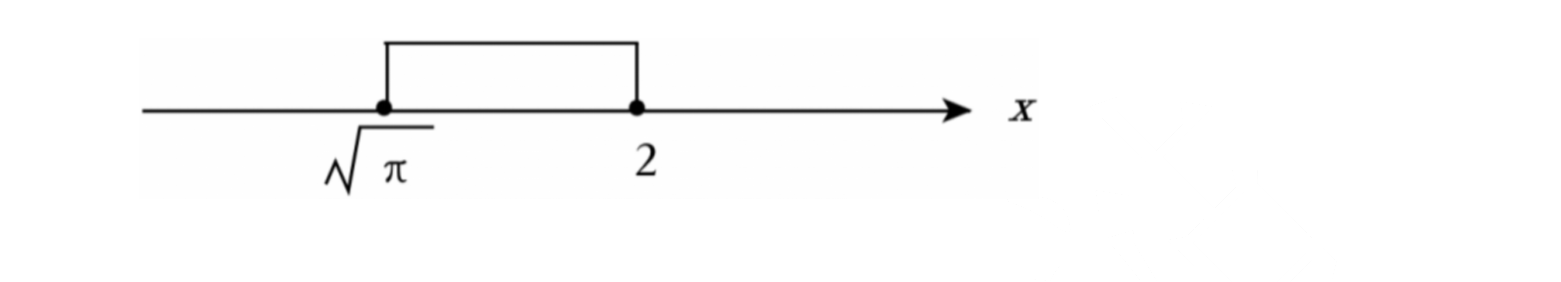
\includegraphics[width=0.72\textwidth]{figures/gao74_q8_numline.png}
\end{center}
\step{所以数形结合得所求集为 $[\sqrt\pi,2]$.}
\solend
\fi

\item 已知集合 $A=\{x\mid(a-1)x^2+3x-3=0,\,x\in\R\}$ 有且仅有一个真子集，则实数 $a=$\blankline[4.4em].

\ifanswer
\solbegin
\step{因为集合 $A=\{x\mid(a-1)x^2+3x-3=0,\,x\in\R\}$ 有且仅有一个真子集，}
\step{所以 $(a-1)x^2+3x-3=0$ 只有一个解，}
\step{所以 $a=1$ 或 $\begin{cases}a\neq1\\ \Delta=3^2-4(a-1)\times(-3)=0\end{cases}$，解得 $a=1$ 或 $a=\dfrac14$.}
\solend
\fi

\item 已知全集 $U=\{(x,y)\mid x,y\in\R\}$，若集合 $A\subseteq U$，且对任意 $(x_1,y_1)\in A$，均存在 $(x_2,y_2)\in A$，使得 $x_1y_2+x_2y_1=0$，则称集合 $A$ 为“对称对点集”. 给出如下集合：

（1）$A=\{(x,y)\mid x,y\in\Z\}$；

（2）$A=\left\{(x,y)\,\middle|\,y=\begin{cases}x+1,&x\geqslant0\\ -x+1,&x<0\end{cases},\ x\in\R,\ x\neq0\right\}$；

（3）$A=\{(x,y)\mid y=x+2,\,x\in\R\}$；

（4）$A=\left\{(x,y)\,\middle|\,y=\dfrac1x,\ x\in\R,\ x\neq0\right\}$.

其中是“对称对点集”的序号为\blankline[4.4em]（写出所有正确的序号）.

\ifanswer
\solbegin
\stepm{(1)}{因为 $0\in\Z$，所以 $(0,0)\in A$.}
\step{对任意 $(x_1,y_1)\in A$，取 $(x_2,y_2)=(0,0)\in A$，}
\step{都有 $x_1\times0+0\times y_1=0$，所以（1）是对称对点集.}
\stepm{(2)}{当 $x_1>0$ 时 $y_1=x_1+1$，取 $x_2=-x_1<0$、$y_2=-x_2+1=x_1+1=y_1$，}
\step{则 $(x_2,y_2)\in A$，且 $x_1y_2+x_2y_1=x_1y_1-x_1y_1=0$；}
\step{当 $x_1<0$ 时同理取 $x_2=-x_1>0$、$y_2=x_2+1=y_1$，}
\step{也有 $(x_2,y_2)\in A$ 且 $x_1y_2+x_2y_1=0$；所以（2）是对称对点集.}
\stepm{(3)}{取 $A$ 中的点 $(-1,1)$. 若存在 $(x_2,y_2)\in A$ 使 $(-1)\cdot y_2+x_2\cdot1=0$，}
\step{则 $y_2=x_2$，但 $A$ 中点的坐标满足 $y=x+2$，两者矛盾，}
\step{所以（3）不是对称对点集.}
\stepm{(4)}{设 $(x_1,y_1)\in A$，则 $x_1\neq0$ 且 $y_1=\dfrac1{x_1}$，}
\step{若存在 $(x_2,y_2)\in A$ 使 $x_1y_2+x_2y_1=0$，}
\step{把 $y_1=\dfrac1{x_1}$、$y_2=\dfrac1{x_2}$（$x_2\neq0$）代入得 $\dfrac{x_1}{x_2}+\dfrac{x_2}{x_1}=0$，即 $x_1^2+x_2^2=0$，}
\step{于是 $x_1=x_2=0$，与 $x_1\neq0$、$x_2\neq0$ 矛盾，所以（4）不是对称对点集.}
\step{故正确的是①②.}
\solend
\fi

\end{enumerate}

\bigsec{二、选择题}

\begin{enumerate}
\setcounter{enumi}{10}

\item “$x>3$”是“$\dfrac{x-1}{x-3}>0$”的\mbox{（\quad）}

\keepwithprev
A. 充分不必要条件\qquad B. 必要不充分条件\qquad C. 充要条件\qquad D. 既不充分也不必要条件

\ifanswer
\solbegin
\step{由 $\dfrac{x-1}{x-3}>0$ 得 $x>3$ 或 $x<1$，故“$x>3$”是“$\dfrac{x-1}{x-3}>0$”的充分不必要条件.}
\step{故选 $A$.}
\solend
\fi

\item 已知 $a,b,c\in\R$，$b>c$，则下列不等式中恒成立的是\mbox{（\quad）}

\keepwithprev
A. $a+b^2>a+c^2$\qquad B. $a^2+b>a^2+c$\qquad C. $ab^2>ac^2$\qquad D. $a^2b>a^2c$

\ifanswer
\solbegin
\step{对于 $A$，取 $b=1,c=-1$，错误；对于 $B$，由不等式的同向可加性得正确；}
\step{对于 $C$，取 $a=1,b=1,c=-2$，错误；对于 $D$，取 $a=0$，错误.}
\step{故选 $B$.}
\solend
\fi

\item 已知关于 $x$ 的不等式 $x^2-2kx+1>0$ 对于一切实数 $x$ 都成立，则实数 $k$ 的取值范围是\mbox{（\quad）}

\keepwithprev
A. $[-1,1]$\qquad B. $(-1,1)$\qquad C. $(-\infty,-1)\cup(1,+\infty)$\qquad D. $\left(-\dfrac12,\dfrac12\right)$

\ifanswer
\solbegin
\step{因为关于 $x$ 的不等式 $x^2-2kx+1>0$ 对于一切实数 $x$ 都成立，}
\step{所以 $\Delta=(-2k)^2-4<0$，即 $4k^2-4<0$，解得 $-1<k<1$，}
\step{所以实数 $k$ 的取值范围是 $(-1,1)$. 故选 $B$.}
\solend
\fi

\item 某种生产设备购买时费用 $100$ 千元，每年的设备管理费 $8$ 千元，这种生产设备的维修费前 $x(x\in\N)$ 年共 $\dfrac{25}{36}x^2+2x$ 千元，问这种生产设备最多使用\mbox{（\quad）}年报废最合算？（即年平均费用最少）

\keepwithprev
A. $13$\qquad B. $10$\qquad C. $15$\qquad D. $12$

\ifanswer
\solbegin
\step{设使用 $x$ 年报废，则总费用 $S(x)=100+8x+\dfrac{25}{36}x^2+2x=\dfrac{25}{36}x^2+10x+100$，}
\step{则年平均费用为 $y=\dfrac{S(x)}x=\dfrac{25x}{36}+\dfrac{100}x+10\geqslant2\sqrt{\dfrac{25x}{36}\cdot\dfrac{100}x}+10=\dfrac{80}3$，}
\step{当且仅当 $\dfrac{25x}{36}=\dfrac{100}x$，即 $x=12$ 时，取等号，}
\step{故当使用 $12$ 年报废，年平均费用最少. 故选 $D$.}
\solend
\fi

\end{enumerate}

\bigsec{三、解答题}

\begin{enumerate}
\setcounter{enumi}{14}

\item （1）设集合 $A=\{x\mid ax-1=0,\,x\in\R\}$，$B=\{x\mid x^2-3x+2=0,\,x\in\R\}$，若 $A\cap B\neq\varnothing$，求实数 $a$ 的取值范围；

（2）已知一元二次方程 $x^2-mx+m+1=0$ 的两个不等实根为 $x_1$、$x_2$，且 $x_1^2+x_2^2=1$，求实数 $m$ 的值.

\ifanswer
\solbegin
\stepm{(1)}{$B=\{x\mid x^2-3x+2=0,\,x\in\R\}=\{1,2\}$，}
\step{①当 $a=0$ 时，方程 $0\cdot x-1=0$ 无解，$A=\varnothing$，$A\cap B=\varnothing$，不符合题意；}
\step{②当 $a\neq0$ 时，$A=\left\{\dfrac1a\right\}$. $A\cap B\neq\varnothing$，}
\step{则 $\dfrac1a\in B$，即 $\dfrac1a=1$ 或 $\dfrac1a=2$，解得 $a=1$ 或 $\dfrac12$；}
\stepm{(2)}{方程 $x^2-mx+m+1=0$ 有两个不等实根，}
\step{则 $\Delta=m^2-4(m+1)>0$，解得 $m>2+2\sqrt2$ 或 $m<2-2\sqrt2$，}
\step{由韦达定理得 $x_1+x_2=m$，$x_1x_2=m+1$，$x_1^2+x_2^2=1$，}
\step{则 $(x_1+x_2)^2-2x_1x_2=m^2-2(m+1)=1$，解得 $m=-1$ 或 $m=3$（舍去），}
\step{综上所述，$m=-1$.}
\solend
\fi

\ansspace

\item 设全集为 $\R$，已知集合 $A=\{x\mid|x-1|\leqslant3,\,x\in\R\}$，

$B=\{x\mid x^2-2mx+(m-3)(m+3)\leqslant0,\,x\in\R\}$.

（1）若 $A\cap B=[0,4]$，求实数 $m$ 的值；

（2）若 $A\cap\overline{B}=A$，求实数 $m$ 的取值范围.

\ifanswer
\solbegin
\stepm{(1)}{$A=\{x\mid|x-1|\leqslant3\}=\{x\mid-2\leqslant x\leqslant4\}$，}
\step{$B=\{x\mid x^2-2mx+(m-3)(m+3)\leqslant0\}=\{x\mid m-3\leqslant x\leqslant m+3\}$，}
\step{若 $A\cap B=[0,4]$，则 $m-3=0$，即 $m=3$；}
\stepm{(2)}{若 $A\cap\overline{B}=A$，则 $A\subseteq\overline{B}$，$\overline{B}=\{x\mid x>m+3\text{ 或 }x<m-3\}$，}
\step{所以 $m+3<-2$ 或 $m-3>4$，解得 $m<-5$ 或 $m>7$，}
\step{实数 $m$ 的取值范围为 $\{m\mid m<-5\text{ 或 }m>7\}$.}
\solend
\fi

\ansspace

\item （1）已知 $a$、$b$ 为正实数，若 $a+b>4$，试用反证法证明：$\dfrac{a}{b+2}$ 和 $\dfrac{b}{a+2}$ 中至少有一个\mbox{大于 $\dfrac12$}；

（2）设 $x$、$y$ 为正实数，$m=\sqrt{2x}+\sqrt{2y}$，$n=\sqrt{x^2+5xy+y^2}$，试比较 $m$、$n$ 的大小，并说明理由.

\ifanswer
\solbegin
\stepm{(1)}{假设 $\dfrac{a}{b+2}\leqslant\dfrac12$ 且 $\dfrac{b}{a+2}\leqslant\dfrac12$，}
\step{又由 $a$、$b$ 为正实数，则有 $2a\leqslant b+2$ 且 $2b\leqslant a+2$，}
\step{两式相加，有 $2a+2b\leqslant a+b+4$，变形得 $a+b\leqslant4$，}
\step{与已知 $a+b>4$ 相矛盾，即假设 $\dfrac{a}{b+2}\leqslant\dfrac12$ 且 $\dfrac{b}{a+2}\leqslant\dfrac12$ 不成立，}
\step{故 $\dfrac{a}{b+2}$ 和 $\dfrac{b}{a+2}$ 中至少有一个\mbox{大于 $\dfrac12$}；}
\stepm{(2)}{$m>n$，理由：$x$、$y$ 为正实数，$m=\sqrt{2x}+\sqrt{2y}$，$n=\sqrt{x^2+5xy+y^2}$，}
\step{则 $m^2=(\sqrt{2x}+\sqrt{2y})^2=2x^2+2y^2+4xy$，$n^2=x^2+y^2+5xy$，}
\step{则有 $m^2-n^2=2x^2+2y^2+4xy-x^2-y^2-5xy=x^2+y^2-xy$}
\step{$=\left(x-\dfrac y2\right)^2+\dfrac{3y^2}4$，}
\step{又 $x$、$y$ 为正实数，则 $m^2-n^2>0$，即 $m^2>n^2$，必有 $m>n$，结论成立.}
\solend
\fi

\ansspace

\item 已知集合 $A=\{a_1,a_2,a_3,\cdots,a_n\}$，$a_i$ 为正整数（$i=1,2,\cdots,n$）.

（1）设 $n=3$，$a_1=1$，$a_2=3$，$a_3=9$，$B=\{a_i+a_j\mid1\leqslant i<j\leqslant3,\,i,j\in\N^*\}$，若互不相同的三个实数 $b_1$、$b_2$、$b_3$，满足 $\{b_i+b_j\mid1\leqslant i<j\leqslant3,\,i,j\in\N^*\}=B$，求有序数组 $(b_1,b_2,b_3)$；

（2）设 $n=4$，$C=\{a_1^2,a_2^2,a_3^2,a_4^2\}$，其中 $a_1<a_2<a_3<a_4$，$A\cap C=\{a_1,a_4\}$，且 $a_1+a_4=10$，$A\cup C$ 中所有元素之和为 $124$，求集合 $A$；

（3）设 $n=2$，有 $7$ 个互不相同的集合 $A$ 分别记为 $A_1$、$A_2$、$A_3$、$\cdots$、$A_7$，且 $A_1\cap A_7=\varnothing$、$A_i\cap A_{i+1}=\varnothing\,(i=1,2,3,\cdots,6)$，记 $D=A_1\cup A_2\cup A_3\cup\cdots\cup A_7$，求 $D$ 中元素个数的最小值.

\ifanswer
\solbegin
\stepm{(1)}{$B=\{a_i+a_j\mid1\leqslant i<j\leqslant3,\,i,j\in\N^*\}=\{1+3,1+9,3+9\}=\{4,10,12\}$，}
\step{由题意，不妨设 $b_1<b_2<b_3$，}
\step{则三个数两两之和为 $\begin{cases}b_1+b_2=4\\ b_1+b_3=10\\ b_2+b_3=12\end{cases}$，解得 $\begin{cases}b_1=1\\ b_2=3\\ b_3=9\end{cases}$，}
\step{所以满足条件的有序数组为 $1$，$3$，$9$ 三个数字的全部排列，}
\step{所以有序数组 $(b_1,b_2,b_3)$ 为 $(1,3,9),(1,9,3),(3,1,9),(3,9,1),(9,1,3),(9,3,1)$；}
\stepm{(2)}{因为 $A\cap C=\{a_1,a_4\}$，所以 $a_1\in C$，$a_4\in C$，}
\step{所以 $a_1$ 是集合 $A$ 中某个正整数的平方，}
\step{又因为 $a_1$ 是最小的正整数，所以只能是 $a_1=1$，此时满足 $1=1^2$.}
\step{又 $a_1+a_4=10$，所以 $a_4=9$，所以 $9$ 也是集合 $A$ 中某个正整数的平方，}
\step{因为 $3^2=9$，所以 $3\in A$，则有 $a_2=3$ 或 $a_3=3$.}
\step{若 $a_3=3$，则 $A=\{1,a_2,3,9\}$，$C=\{1^2,a_2^2,3^2,9^2\}=\{1,a_2^2,9,81\}$，}
\step{因为 $a_1<a_2<a_3<a_4$，且 $a_2$ 为正整数，所以只能是 $a_2=2$，}
\step{故 $A=\{1,2,3,9\}$，$C=\{1,4,9,81\}$，$A\cap C=\{1,9\}$，符合题意，}
\step{则 $A\cup C=\{1,2,3,4,9,81\}$，此时 $1+2+3+4+9+81=100\neq124$，}
\step{故 $a_3=3$ 不符合题意，所以只能 $a_2=3$，}
\step{故 $A=\{1,3,a_3,9\}$，$C=\{1^2,3^2,a_3^2,9^2\}$，此时 $A\cup C=\{1,3,a_3,9,a_3^2,81\}$，}
\step{则有 $1+3+a_3+9+a_3^2+81=124$，}
\step{即 $a_3^2+a_3-30=(a_3+6)(a_3-5)=0$，解得正整数 $a_3=5$，}
\step{此时 $A=\{1,3,5,9\}$，$C=\{1,9,25,81\}$，$A\cup C=\{1,3,5,9,25,81\}$，}
\step{满足 $A\cap C=\{1,9\}$，$A\cup C$ 中所有元素之和为 $1+3+5+9+25+81=124$，}
\step{故 $A=\{1,3,5,9\}$；}
\stepm{(3)}{当 $n=2$ 时，每个集合 $A_i(i=1,2,\cdots,7)$ 均为含有 $2$ 个元素的二元集合，}
\step{设 $D$ 中元素个数为 $m$，}
\step{若 $m\leqslant4$，从 $m$ 个元素中最多能得到 $\dfrac{4\times3}2=6$ 个不同二元集合，不足 $7$ 个，}
\step{故 $m\leqslant4$ 不可能.}
\step{若 $m=5$，则有 $\dfrac{5\times4}2=10$ 个不同二元集合，数量超过 $7$ 个，符合要求.}
\step{因为 $A_i\cap A_{i+1}=\varnothing(i=1,2,3,\cdots,6)$，$A_1\cap A_7=\varnothing$，}
\step{即要求 $7$ 个互不相同的二元集合排成环，}
\step{且相邻（含首尾）集合交集为空集.}
\needvspace{12\baselineskip}
\step{假设 $m=5$，不妨设 $A_1(1,2)$、$A_2(3,4)$、$A_3(1,5)$，则：}
\begin{center}
\renewcommand{\arraystretch}{1.9}
\begin{tabular}{|c|c|c|c|c|}
\hline
$A_4(2,3)$ & $A_5(1,4)$ & $A_6(2,5)$ & $A_7(1,3)$ & 与 $A_1$ 矛盾\\
\hline
 &  & $A_6(3,5)$ & $A_7(2,4)$ & 与 $A_1$ 矛盾\\
\hline
 & $A_5(4,5)$ & $A_6(1,3)$ & $A_7(2,5)$ 或 $A_7(2,4)$ & 与 $A_1$ 矛盾\\
\hline
$A_4(2,4)$ & $A_5(1,3)$ & $A_6(2,5)$ & $A_7(1,4)$ & 与 $A_1$ 矛盾\\
\hline
 &  & $A_6(4,5)$ & $A_7(2,3)$ & 与 $A_1$ 矛盾\\
\hline
 & $A_5(3,5)$ & $A_6(1,4)$ & $A_7(2,3)$ 或 $A_7(2,5)$ & 与 $A_1$ 矛盾\\
\hline
\end{tabular}
\end{center}
\step{故 $m=5$ 不可能.}
\step{综上，$m\geqslant6$，取 $D=\{1,2,3,4,5,6\}$，}
\step{令 $A_1=\{1,2\},A_2=\{3,4\},A_3=\{1,5\},A_4=\{2,4\},A_5=\{3,6\},A_6=\{1,4\}$，}
\step{$A_7=\{5,6\}$，此时 $A_1$、$A_2$、$\cdots$、$A_7$ 是 $7$ 个互不相同的二元集合，}
\step{且 $A_1\cap A_2=\varnothing$，$A_2\cap A_3=\varnothing$，$A_3\cap A_4=\varnothing$，$A_4\cap A_5=\varnothing$，}
\step{$A_5\cap A_6=\varnothing$，$A_6\cap A_7=\varnothing$，$A_7\cap A_1=\varnothing$，满足全部条件，}
\step{故 $D$ 中元素个数的最小值为 $6$.}
\solend
\fi

\ansspace*[7]

\end{enumerate}

\end{document}
"
%
% 原始材料：微信公众号“魔都数学加油站”文章，连载“27学年高一74”；
% 原文标题“27学年高一74——2026-2027年上海市宜川中学高一上10月月考”；
% 原文链接：https://mp.weixin.qq.com/s/ymsl2bmkBRY6ZPDiUFCDTA。
% 页面标注发布时间 2026-10-22 21:45（上海）。
% 正文为 9 张 PNG 页（`原图/高一74_宜川中学_10月月考/01..09.png`）：
% 第 1、2、3 页为 4762×6735，其余 6 页为 2560×3620，均按页序读取。
% 9 页全为试卷正文页（卷首标题在第 1 页页顶，卷末第 18 题 (3) 解析止于第 9 页），
% 无封面页、目录页、二维码或宣传页。粉色斜排“魔都数学加油站”为卷面水印，未录入。
%
% 卷首标题：照卷面印作“2026-2027 年宜川中学高一上 10 月月考”（黑体加粗一行）。
% 原卷年份区间用半角连字符，本稿按全稿惯例排 en dash；原卷无副标题。
%
% 篇幅与题号：原卷自第 3 题起编号（第 1、2 题不在本卷内）。填空题 3—10（8 题）、
% 选择题 11—14（4 题）、解答题 15—18（4 题），共 16 题。本稿沿用原节与原题号，
% 只改排为全稿统一的大节样式。
%
% 讲评版：原卷第 3 题只印【答案】（“{(1,1)}”），本稿只给 \ans{}；其余 15 题均印
% 【解析】，用 \solbegin…\solend。四道选择题的作答括号原卷即留空，答案写在解析末句
% “故选 A／B／B／D”，照录在解析内，不另提 \ans{}。
%
% 副标题：原卷未印副标题。本稿按“知识模块”口径标作“集合与常用逻辑用语、不等式”：
% 16 题中集合与常用逻辑用语 7 题（第 3、9、10、15、16、18 题及第 17 题的反证法），
% 不等式 9 题（第 4—8、11—14、17 题），两类均确有分量，故并标。口径同 高一63、高一68—73。
%
% 与原卷的排版差异：
%   ① 原卷每题下直接印【答案】/【解析】，本稿按全稿惯例将答案与解析置于答案版；
%   ② 原卷未印副标题，本稿按“知识模块”口径补出；
%   ③ 原卷填空横线约四个字宽，本稿按全稿惯例统一排 \blankline[4.4em]；
%   ④ 原卷数集记号排斜体 $R$、$Z$、$N$（第 8、9、10、14—18 题），本稿按全稿惯例
%      改用 $\R$、$\Z$、$\N$（同 高一68—73）；第 18 题的正整数集合作 $\N^*$，照录；
%   ⑤ 原卷句末标点多为西文句点，均逐处照录；
%   ⑥ 第 15—18 题的子问原卷印作“（1）…（2）…”，本稿按 高一69—73 成例用行内
%      “（1）（2）（3）”段，解析中的子问标号用 \stepm{(1)}{…}；
%   ⑦ 每道解答题原卷未留作答空白，本稿按全稿惯例加 \ansspace（末题用 \ansspace*）；
%   ⑧ 选择题的作答括号原卷排半角“(    )”，本稿按全稿惯例排 \mbox{（\quad）}；
%      选项行排照原卷——第 11、13 题一行四条，第 12、14 题一行四条；
%   ⑨ 第 9、14、18 题解析中的不等式组／方程组，原卷均排作“{”连接的多行式，
%      本稿按全稿惯例排 cases；
%   ⑩ 第 8 题解析有一幅数轴图：原卷印在【解析】第 2 行之后，题干无“如图”二字。
%      本稿按原卷截图裁取（`figures/gao74_q8_numline.png`，由第 2 页原图裁出、
%      去除粉色水印后转灰度，未放大），放在答案版解析第 2 条之后；
%   ⑪ 第 18 题 (3) 解析中有一张 5 列 6 行的枚举表（原卷无表头、左侧两列留空以表示
%      沿用上格的 $A_4$／$A_5$），本稿照原卷排成同样的空格表，未加表头、未合并单元格。
%
% 原卷笔误/存疑（均照录未改，正文对应处另有 % 注）：
%   ① 第 14 题题干“维修费前 $x(x\in N)$ 年共 $\dfrac{25}{36}x^2+2x$ 千元”中的
%      $N$ 原卷排斜体，按全稿惯例改 $\N$，含义不变；
%   ② 第 18 题 (3) 的枚举表第 1—3 行与第 4—6 行分属“$A_5(1,4)$”“$A_5(1,3)$”两种
%      情形，原卷只在首行重复写 $A_4$、$A_5$，其余留空；本稿照录留空，未补字。
%
% 行数核对：逐题数 \step/\stepm 条数与原卷【解析】印刷行数，15 题逐一相符，
% 合计 104 条 / 104 行（Q4：1；Q5：2；Q6：3；Q7：3；Q8：3；Q9：3；Q10：15；
% Q11：2；Q12：3；Q13：3；Q14：4；Q15：9；Q16：6；Q17：10；Q18：37）。
% 另第 3 题只印【答案】，提 \ans{}，不计入 \step 账。
%
% 插图：第 8 题解析的数轴图，见上⑩；全卷题干无其他配图。
%
\documentclass[a4paper,11pt]{article}
\usepackage{common}

\begin{document}

\examtitlest[3]{2026--2027 年宜川中学高一上 10 月月考}{集合与常用逻辑用语、不等式}

\bigsec{一、填空题}

\begin{enumerate}
\setcounter{enumi}{2}

\item 已知集合 $A=\{(x,y)\mid y=x\}$，集合 $B=\{(x,y)\mid y=2-x\}$，则 $A\cap B=$\blankline[4.4em].

\ifanswer
\ans{$\{(1,1)\}$}
\fi

\item 已知 $a=\log_3 2$，$b=\log_3 8$，则 $3^{2a-b}=$\blankline[4.4em].

\ifanswer
\solbegin
\step{由 $a=\log_3 2$，$b=\log_3 8$，得 $3^a=2$，$3^b=8$，则 $3^{2a-b}=\dfrac{(3^a)^2}{3^b}=\dfrac48=\dfrac12$.}
\solend
\fi

\item 已知等式 $2x^2+3x+5=a(2x+1)(x+1)+c$ 恒成立，则实数 $c=$\blankline[4.4em].

\ifanswer
\solbegin
\step{$2x^2+3x+5=a(2x+1)(x+1)+c=2ax^2+3ax+a+c$，}
\step{则 $\begin{cases}2a=2\\ 3a=3\\ a+c=5\end{cases}$，解得 $c=4$.}
\solend
\fi

\item 已知 $x>0$，$y>0$，且 $\dfrac9x+\dfrac1y=1$，则 $x\cdot y$ 的最小值是\blankline[4.4em].

\ifanswer
\solbegin
\step{$x>0$，$y>0$，且 $1=\dfrac9x+\dfrac1y\geqslant2\sqrt{\dfrac9{xy}}$，}
\step{当且仅当 $x=9y$，即 $y=2$，$x=18$ 时取等号，所以 $xy\geqslant36$，}
\step{则 $x\cdot y$ 的最小值为 $36$.}
\solend
\fi

\item 已知关于 $x$ 的不等式 $x^2+bx+c>0$（$b$、$c$ 为实数）的解集为 $(-\infty,-2)\cup(3,+\infty)$，则不等式 $cx^2-bx+1\leqslant0$ 的解集为\blankline[4.4em].

\ifanswer
\solbegin
\step{由已知得 $-2$、$3$ 为方程 $x^2+bx+c=0$ 的根，所以 $-2+3=-b$，$-2\times3=c$，}
\step{即 $b=-1$，$c=-6$，所以不等式 $cx^2-bx+1\leqslant0$ 可变形为 $-6x^2+x+1\leqslant0$，}
\step{即 $6x^2-x-1\geqslant0$，解得 $x\leqslant-\dfrac13$ 或 $x\geqslant\dfrac12$，所以解集为 $\left(-\infty,-\dfrac13\right]\cup\left[\dfrac12,+\infty\right)$.}
\solend
\fi

\item 设 $x\in\R$，则方程 $|x-2|+|\sqrt\pi-x|=2-\sqrt\pi$ 的解集为\blankline[4.4em].

\ifanswer
\solbegin
\step{因为方程 $|x-2|+|\sqrt\pi-x|=2-\sqrt\pi$ 可化为 $|x-2|+|x-\sqrt\pi|=2-\sqrt\pi$，}
\needvspace{8\baselineskip}
\step{其表示数轴上实数 $x$ 到 $\sqrt\pi$ 与 $2$ 的距离之和等于 $2-\sqrt\pi$，如图：}
\begin{center}
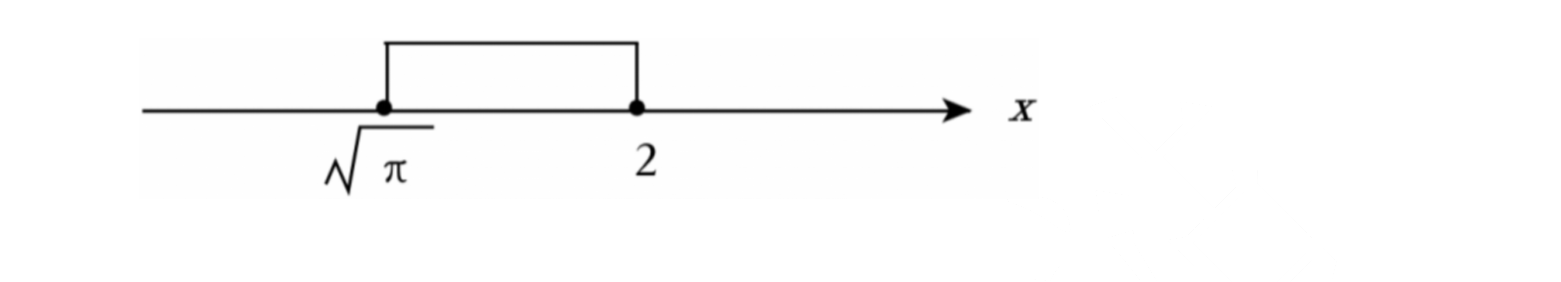
\includegraphics[width=0.72\textwidth]{figures/gao74_q8_numline.png}
\end{center}
\step{所以数形结合得所求集为 $[\sqrt\pi,2]$.}
\solend
\fi

\item 已知集合 $A=\{x\mid(a-1)x^2+3x-3=0,\,x\in\R\}$ 有且仅有一个真子集，则实数 $a=$\blankline[4.4em].

\ifanswer
\solbegin
\step{因为集合 $A=\{x\mid(a-1)x^2+3x-3=0,\,x\in\R\}$ 有且仅有一个真子集，}
\step{所以 $(a-1)x^2+3x-3=0$ 只有一个解，}
\step{所以 $a=1$ 或 $\begin{cases}a\neq1\\ \Delta=3^2-4(a-1)\times(-3)=0\end{cases}$，解得 $a=1$ 或 $a=\dfrac14$.}
\solend
\fi

\item 已知全集 $U=\{(x,y)\mid x,y\in\R\}$，若集合 $A\subseteq U$，且对任意 $(x_1,y_1)\in A$，均存在 $(x_2,y_2)\in A$，使得 $x_1y_2+x_2y_1=0$，则称集合 $A$ 为“对称对点集”. 给出如下集合：

（1）$A=\{(x,y)\mid x,y\in\Z\}$；

（2）$A=\left\{(x,y)\,\middle|\,y=\begin{cases}x+1,&x\geqslant0\\ -x+1,&x<0\end{cases},\ x\in\R,\ x\neq0\right\}$；

（3）$A=\{(x,y)\mid y=x+2,\,x\in\R\}$；

（4）$A=\left\{(x,y)\,\middle|\,y=\dfrac1x,\ x\in\R,\ x\neq0\right\}$.

其中是“对称对点集”的序号为\blankline[4.4em]（写出所有正确的序号）.

\ifanswer
\solbegin
\stepm{(1)}{因为 $0\in\Z$，所以 $(0,0)\in A$.}
\step{对任意 $(x_1,y_1)\in A$，取 $(x_2,y_2)=(0,0)\in A$，}
\step{都有 $x_1\times0+0\times y_1=0$，所以（1）是对称对点集.}
\stepm{(2)}{当 $x_1>0$ 时 $y_1=x_1+1$，取 $x_2=-x_1<0$、$y_2=-x_2+1=x_1+1=y_1$，}
\step{则 $(x_2,y_2)\in A$，且 $x_1y_2+x_2y_1=x_1y_1-x_1y_1=0$；}
\step{当 $x_1<0$ 时同理取 $x_2=-x_1>0$、$y_2=x_2+1=y_1$，}
\step{也有 $(x_2,y_2)\in A$ 且 $x_1y_2+x_2y_1=0$；所以（2）是对称对点集.}
\stepm{(3)}{取 $A$ 中的点 $(-1,1)$. 若存在 $(x_2,y_2)\in A$ 使 $(-1)\cdot y_2+x_2\cdot1=0$，}
\step{则 $y_2=x_2$，但 $A$ 中点的坐标满足 $y=x+2$，两者矛盾，}
\step{所以（3）不是对称对点集.}
\stepm{(4)}{设 $(x_1,y_1)\in A$，则 $x_1\neq0$ 且 $y_1=\dfrac1{x_1}$，}
\step{若存在 $(x_2,y_2)\in A$ 使 $x_1y_2+x_2y_1=0$，}
\step{把 $y_1=\dfrac1{x_1}$、$y_2=\dfrac1{x_2}$（$x_2\neq0$）代入得 $\dfrac{x_1}{x_2}+\dfrac{x_2}{x_1}=0$，即 $x_1^2+x_2^2=0$，}
\step{于是 $x_1=x_2=0$，与 $x_1\neq0$、$x_2\neq0$ 矛盾，所以（4）不是对称对点集.}
\step{故正确的是①②.}
\solend
\fi

\end{enumerate}

\bigsec{二、选择题}

\begin{enumerate}
\setcounter{enumi}{10}

\item “$x>3$”是“$\dfrac{x-1}{x-3}>0$”的\mbox{（\quad）}

\keepwithprev
A. 充分不必要条件\qquad B. 必要不充分条件\qquad C. 充要条件\qquad D. 既不充分也不必要条件

\ifanswer
\solbegin
\step{由 $\dfrac{x-1}{x-3}>0$ 得 $x>3$ 或 $x<1$，故“$x>3$”是“$\dfrac{x-1}{x-3}>0$”的充分不必要条件.}
\step{故选 $A$.}
\solend
\fi

\item 已知 $a,b,c\in\R$，$b>c$，则下列不等式中恒成立的是\mbox{（\quad）}

\keepwithprev
A. $a+b^2>a+c^2$\qquad B. $a^2+b>a^2+c$\qquad C. $ab^2>ac^2$\qquad D. $a^2b>a^2c$

\ifanswer
\solbegin
\step{对于 $A$，取 $b=1,c=-1$，错误；对于 $B$，由不等式的同向可加性得正确；}
\step{对于 $C$，取 $a=1,b=1,c=-2$，错误；对于 $D$，取 $a=0$，错误.}
\step{故选 $B$.}
\solend
\fi

\item 已知关于 $x$ 的不等式 $x^2-2kx+1>0$ 对于一切实数 $x$ 都成立，则实数 $k$ 的取值范围是\mbox{（\quad）}

\keepwithprev
A. $[-1,1]$\qquad B. $(-1,1)$\qquad C. $(-\infty,-1)\cup(1,+\infty)$\qquad D. $\left(-\dfrac12,\dfrac12\right)$

\ifanswer
\solbegin
\step{因为关于 $x$ 的不等式 $x^2-2kx+1>0$ 对于一切实数 $x$ 都成立，}
\step{所以 $\Delta=(-2k)^2-4<0$，即 $4k^2-4<0$，解得 $-1<k<1$，}
\step{所以实数 $k$ 的取值范围是 $(-1,1)$. 故选 $B$.}
\solend
\fi

\item 某种生产设备购买时费用 $100$ 千元，每年的设备管理费 $8$ 千元，这种生产设备的维修费前 $x(x\in\N)$ 年共 $\dfrac{25}{36}x^2+2x$ 千元，问这种生产设备最多使用\mbox{（\quad）}年报废最合算？（即年平均费用最少）

\keepwithprev
A. $13$\qquad B. $10$\qquad C. $15$\qquad D. $12$

\ifanswer
\solbegin
\step{设使用 $x$ 年报废，则总费用 $S(x)=100+8x+\dfrac{25}{36}x^2+2x=\dfrac{25}{36}x^2+10x+100$，}
\step{则年平均费用为 $y=\dfrac{S(x)}x=\dfrac{25x}{36}+\dfrac{100}x+10\geqslant2\sqrt{\dfrac{25x}{36}\cdot\dfrac{100}x}+10=\dfrac{80}3$，}
\step{当且仅当 $\dfrac{25x}{36}=\dfrac{100}x$，即 $x=12$ 时，取等号，}
\step{故当使用 $12$ 年报废，年平均费用最少. 故选 $D$.}
\solend
\fi

\end{enumerate}

\bigsec{三、解答题}

\begin{enumerate}
\setcounter{enumi}{14}

\item （1）设集合 $A=\{x\mid ax-1=0,\,x\in\R\}$，$B=\{x\mid x^2-3x+2=0,\,x\in\R\}$，若 $A\cap B\neq\varnothing$，求实数 $a$ 的取值范围；

（2）已知一元二次方程 $x^2-mx+m+1=0$ 的两个不等实根为 $x_1$、$x_2$，且 $x_1^2+x_2^2=1$，求实数 $m$ 的值.

\ifanswer
\solbegin
\stepm{(1)}{$B=\{x\mid x^2-3x+2=0,\,x\in\R\}=\{1,2\}$，}
\step{①当 $a=0$ 时，方程 $0\cdot x-1=0$ 无解，$A=\varnothing$，$A\cap B=\varnothing$，不符合题意；}
\step{②当 $a\neq0$ 时，$A=\left\{\dfrac1a\right\}$. $A\cap B\neq\varnothing$，}
\step{则 $\dfrac1a\in B$，即 $\dfrac1a=1$ 或 $\dfrac1a=2$，解得 $a=1$ 或 $\dfrac12$；}
\stepm{(2)}{方程 $x^2-mx+m+1=0$ 有两个不等实根，}
\step{则 $\Delta=m^2-4(m+1)>0$，解得 $m>2+2\sqrt2$ 或 $m<2-2\sqrt2$，}
\step{由韦达定理得 $x_1+x_2=m$，$x_1x_2=m+1$，$x_1^2+x_2^2=1$，}
\step{则 $(x_1+x_2)^2-2x_1x_2=m^2-2(m+1)=1$，解得 $m=-1$ 或 $m=3$（舍去），}
\step{综上所述，$m=-1$.}
\solend
\fi

\ansspace

\item 设全集为 $\R$，已知集合 $A=\{x\mid|x-1|\leqslant3,\,x\in\R\}$，

$B=\{x\mid x^2-2mx+(m-3)(m+3)\leqslant0,\,x\in\R\}$.

（1）若 $A\cap B=[0,4]$，求实数 $m$ 的值；

（2）若 $A\cap\overline{B}=A$，求实数 $m$ 的取值范围.

\ifanswer
\solbegin
\stepm{(1)}{$A=\{x\mid|x-1|\leqslant3\}=\{x\mid-2\leqslant x\leqslant4\}$，}
\step{$B=\{x\mid x^2-2mx+(m-3)(m+3)\leqslant0\}=\{x\mid m-3\leqslant x\leqslant m+3\}$，}
\step{若 $A\cap B=[0,4]$，则 $m-3=0$，即 $m=3$；}
\stepm{(2)}{若 $A\cap\overline{B}=A$，则 $A\subseteq\overline{B}$，$\overline{B}=\{x\mid x>m+3\text{ 或 }x<m-3\}$，}
\step{所以 $m+3<-2$ 或 $m-3>4$，解得 $m<-5$ 或 $m>7$，}
\step{实数 $m$ 的取值范围为 $\{m\mid m<-5\text{ 或 }m>7\}$.}
\solend
\fi

\ansspace

\item （1）已知 $a$、$b$ 为正实数，若 $a+b>4$，试用反证法证明：$\dfrac{a}{b+2}$ 和 $\dfrac{b}{a+2}$ 中至少有一个\mbox{大于 $\dfrac12$}；

（2）设 $x$、$y$ 为正实数，$m=\sqrt{2x}+\sqrt{2y}$，$n=\sqrt{x^2+5xy+y^2}$，试比较 $m$、$n$ 的大小，并说明理由.

\ifanswer
\solbegin
\stepm{(1)}{假设 $\dfrac{a}{b+2}\leqslant\dfrac12$ 且 $\dfrac{b}{a+2}\leqslant\dfrac12$，}
\step{又由 $a$、$b$ 为正实数，则有 $2a\leqslant b+2$ 且 $2b\leqslant a+2$，}
\step{两式相加，有 $2a+2b\leqslant a+b+4$，变形得 $a+b\leqslant4$，}
\step{与已知 $a+b>4$ 相矛盾，即假设 $\dfrac{a}{b+2}\leqslant\dfrac12$ 且 $\dfrac{b}{a+2}\leqslant\dfrac12$ 不成立，}
\step{故 $\dfrac{a}{b+2}$ 和 $\dfrac{b}{a+2}$ 中至少有一个\mbox{大于 $\dfrac12$}；}
\stepm{(2)}{$m>n$，理由：$x$、$y$ 为正实数，$m=\sqrt{2x}+\sqrt{2y}$，$n=\sqrt{x^2+5xy+y^2}$，}
\step{则 $m^2=(\sqrt{2x}+\sqrt{2y})^2=2x^2+2y^2+4xy$，$n^2=x^2+y^2+5xy$，}
\step{则有 $m^2-n^2=2x^2+2y^2+4xy-x^2-y^2-5xy=x^2+y^2-xy$}
\step{$=\left(x-\dfrac y2\right)^2+\dfrac{3y^2}4$，}
\step{又 $x$、$y$ 为正实数，则 $m^2-n^2>0$，即 $m^2>n^2$，必有 $m>n$，结论成立.}
\solend
\fi

\ansspace

\item 已知集合 $A=\{a_1,a_2,a_3,\cdots,a_n\}$，$a_i$ 为正整数（$i=1,2,\cdots,n$）.

（1）设 $n=3$，$a_1=1$，$a_2=3$，$a_3=9$，$B=\{a_i+a_j\mid1\leqslant i<j\leqslant3,\,i,j\in\N^*\}$，若互不相同的三个实数 $b_1$、$b_2$、$b_3$，满足 $\{b_i+b_j\mid1\leqslant i<j\leqslant3,\,i,j\in\N^*\}=B$，求有序数组 $(b_1,b_2,b_3)$；

（2）设 $n=4$，$C=\{a_1^2,a_2^2,a_3^2,a_4^2\}$，其中 $a_1<a_2<a_3<a_4$，$A\cap C=\{a_1,a_4\}$，且 $a_1+a_4=10$，$A\cup C$ 中所有元素之和为 $124$，求集合 $A$；

（3）设 $n=2$，有 $7$ 个互不相同的集合 $A$ 分别记为 $A_1$、$A_2$、$A_3$、$\cdots$、$A_7$，且 $A_1\cap A_7=\varnothing$、$A_i\cap A_{i+1}=\varnothing\,(i=1,2,3,\cdots,6)$，记 $D=A_1\cup A_2\cup A_3\cup\cdots\cup A_7$，求 $D$ 中元素个数的最小值.

\ifanswer
\solbegin
\stepm{(1)}{$B=\{a_i+a_j\mid1\leqslant i<j\leqslant3,\,i,j\in\N^*\}=\{1+3,1+9,3+9\}=\{4,10,12\}$，}
\step{由题意，不妨设 $b_1<b_2<b_3$，}
\step{则三个数两两之和为 $\begin{cases}b_1+b_2=4\\ b_1+b_3=10\\ b_2+b_3=12\end{cases}$，解得 $\begin{cases}b_1=1\\ b_2=3\\ b_3=9\end{cases}$，}
\step{所以满足条件的有序数组为 $1$，$3$，$9$ 三个数字的全部排列，}
\step{所以有序数组 $(b_1,b_2,b_3)$ 为 $(1,3,9),(1,9,3),(3,1,9),(3,9,1),(9,1,3),(9,3,1)$；}
\stepm{(2)}{因为 $A\cap C=\{a_1,a_4\}$，所以 $a_1\in C$，$a_4\in C$，}
\step{所以 $a_1$ 是集合 $A$ 中某个正整数的平方，}
\step{又因为 $a_1$ 是最小的正整数，所以只能是 $a_1=1$，此时满足 $1=1^2$.}
\step{又 $a_1+a_4=10$，所以 $a_4=9$，所以 $9$ 也是集合 $A$ 中某个正整数的平方，}
\step{因为 $3^2=9$，所以 $3\in A$，则有 $a_2=3$ 或 $a_3=3$.}
\step{若 $a_3=3$，则 $A=\{1,a_2,3,9\}$，$C=\{1^2,a_2^2,3^2,9^2\}=\{1,a_2^2,9,81\}$，}
\step{因为 $a_1<a_2<a_3<a_4$，且 $a_2$ 为正整数，所以只能是 $a_2=2$，}
\step{故 $A=\{1,2,3,9\}$，$C=\{1,4,9,81\}$，$A\cap C=\{1,9\}$，符合题意，}
\step{则 $A\cup C=\{1,2,3,4,9,81\}$，此时 $1+2+3+4+9+81=100\neq124$，}
\step{故 $a_3=3$ 不符合题意，所以只能 $a_2=3$，}
\step{故 $A=\{1,3,a_3,9\}$，$C=\{1^2,3^2,a_3^2,9^2\}$，此时 $A\cup C=\{1,3,a_3,9,a_3^2,81\}$，}
\step{则有 $1+3+a_3+9+a_3^2+81=124$，}
\step{即 $a_3^2+a_3-30=(a_3+6)(a_3-5)=0$，解得正整数 $a_3=5$，}
\step{此时 $A=\{1,3,5,9\}$，$C=\{1,9,25,81\}$，$A\cup C=\{1,3,5,9,25,81\}$，}
\step{满足 $A\cap C=\{1,9\}$，$A\cup C$ 中所有元素之和为 $1+3+5+9+25+81=124$，}
\step{故 $A=\{1,3,5,9\}$；}
\stepm{(3)}{当 $n=2$ 时，每个集合 $A_i(i=1,2,\cdots,7)$ 均为含有 $2$ 个元素的二元集合，}
\step{设 $D$ 中元素个数为 $m$，}
\step{若 $m\leqslant4$，从 $m$ 个元素中最多能得到 $\dfrac{4\times3}2=6$ 个不同二元集合，不足 $7$ 个，}
\step{故 $m\leqslant4$ 不可能.}
\step{若 $m=5$，则有 $\dfrac{5\times4}2=10$ 个不同二元集合，数量超过 $7$ 个，符合要求.}
\step{因为 $A_i\cap A_{i+1}=\varnothing(i=1,2,3,\cdots,6)$，$A_1\cap A_7=\varnothing$，}
\step{即要求 $7$ 个互不相同的二元集合排成环，}
\step{且相邻（含首尾）集合交集为空集.}
\needvspace{12\baselineskip}
\step{假设 $m=5$，不妨设 $A_1(1,2)$、$A_2(3,4)$、$A_3(1,5)$，则：}
\begin{center}
\renewcommand{\arraystretch}{1.9}
\begin{tabular}{|c|c|c|c|c|}
\hline
$A_4(2,3)$ & $A_5(1,4)$ & $A_6(2,5)$ & $A_7(1,3)$ & 与 $A_1$ 矛盾\\
\hline
 &  & $A_6(3,5)$ & $A_7(2,4)$ & 与 $A_1$ 矛盾\\
\hline
 & $A_5(4,5)$ & $A_6(1,3)$ & $A_7(2,5)$ 或 $A_7(2,4)$ & 与 $A_1$ 矛盾\\
\hline
$A_4(2,4)$ & $A_5(1,3)$ & $A_6(2,5)$ & $A_7(1,4)$ & 与 $A_1$ 矛盾\\
\hline
 &  & $A_6(4,5)$ & $A_7(2,3)$ & 与 $A_1$ 矛盾\\
\hline
 & $A_5(3,5)$ & $A_6(1,4)$ & $A_7(2,3)$ 或 $A_7(2,5)$ & 与 $A_1$ 矛盾\\
\hline
\end{tabular}
\end{center}
\step{故 $m=5$ 不可能.}
\step{综上，$m\geqslant6$，取 $D=\{1,2,3,4,5,6\}$，}
\step{令 $A_1=\{1,2\},A_2=\{3,4\},A_3=\{1,5\},A_4=\{2,4\},A_5=\{3,6\},A_6=\{1,4\}$，}
\step{$A_7=\{5,6\}$，此时 $A_1$、$A_2$、$\cdots$、$A_7$ 是 $7$ 个互不相同的二元集合，}
\step{且 $A_1\cap A_2=\varnothing$，$A_2\cap A_3=\varnothing$，$A_3\cap A_4=\varnothing$，$A_4\cap A_5=\varnothing$，}
\step{$A_5\cap A_6=\varnothing$，$A_6\cap A_7=\varnothing$，$A_7\cap A_1=\varnothing$，满足全部条件，}
\step{故 $D$ 中元素个数的最小值为 $6$.}
\solend
\fi

\ansspace*[7]

\end{enumerate}

\end{document}
"
%
% 原始材料：微信公众号“魔都数学加油站”文章，连载“27学年高一74”；
% 原文标题“27学年高一74——2026-2027年上海市宜川中学高一上10月月考”；
% 原文链接：https://mp.weixin.qq.com/s/ymsl2bmkBRY6ZPDiUFCDTA。
% 页面标注发布时间 2026-10-22 21:45（上海）。
% 正文为 9 张 PNG 页（`原图/高一74_宜川中学_10月月考/01..09.png`）：
% 第 1、2、3 页为 4762×6735，其余 6 页为 2560×3620，均按页序读取。
% 9 页全为试卷正文页（卷首标题在第 1 页页顶，卷末第 18 题 (3) 解析止于第 9 页），
% 无封面页、目录页、二维码或宣传页。粉色斜排“魔都数学加油站”为卷面水印，未录入。
%
% 卷首标题：照卷面印作“2026-2027 年宜川中学高一上 10 月月考”（黑体加粗一行）。
% 原卷年份区间用半角连字符，本稿按全稿惯例排 en dash；原卷无副标题。
%
% 篇幅与题号：原卷自第 3 题起编号（第 1、2 题不在本卷内）。填空题 3—10（8 题）、
% 选择题 11—14（4 题）、解答题 15—18（4 题），共 16 题。本稿沿用原节与原题号，
% 只改排为全稿统一的大节样式。
%
% 讲评版：原卷第 3 题只印【答案】（“{(1,1)}”），本稿只给 \ans{}；其余 15 题均印
% 【解析】，用 \solbegin…\solend。四道选择题的作答括号原卷即留空，答案写在解析末句
% “故选 A／B／B／D”，照录在解析内，不另提 \ans{}。
%
% 副标题：原卷未印副标题。本稿按“知识模块”口径标作“集合与常用逻辑用语、不等式”：
% 16 题中集合与常用逻辑用语 7 题（第 3、9、10、15、16、18 题及第 17 题的反证法），
% 不等式 9 题（第 4—8、11—14、17 题），两类均确有分量，故并标。口径同 高一63、高一68—73。
%
% 与原卷的排版差异：
%   ① 原卷每题下直接印【答案】/【解析】，本稿按全稿惯例将答案与解析置于答案版；
%   ② 原卷未印副标题，本稿按“知识模块”口径补出；
%   ③ 原卷填空横线约四个字宽，本稿按全稿惯例统一排 \blankline[4.4em]；
%   ④ 原卷数集记号排斜体 $R$、$Z$、$N$（第 8、9、10、14—18 题），本稿按全稿惯例
%      改用 $\R$、$\Z$、$\N$（同 高一68—73）；第 18 题的正整数集合作 $\N^*$，照录；
%   ⑤ 原卷句末标点多为西文句点，均逐处照录；
%   ⑥ 第 15—18 题的子问原卷印作“（1）…（2）…”，本稿按 高一69—73 成例用行内
%      “（1）（2）（3）”段，解析中的子问标号用 \stepm{(1)}{…}；
%   ⑦ 每道解答题原卷未留作答空白，本稿按全稿惯例加 \ansspace（末题用 \ansspace*）；
%   ⑧ 选择题的作答括号原卷排半角“(    )”，本稿按全稿惯例排 \mbox{（\quad）}；
%      选项行排照原卷——第 11、13 题一行四条，第 12、14 题一行四条；
%   ⑨ 第 9、14、18 题解析中的不等式组／方程组，原卷均排作“{”连接的多行式，
%      本稿按全稿惯例排 cases；
%   ⑩ 第 8 题解析有一幅数轴图：原卷印在【解析】第 2 行之后，题干无“如图”二字。
%      本稿按原卷截图裁取（`figures/gao74_q8_numline.png`，由第 2 页原图裁出、
%      去除粉色水印后转灰度，未放大），放在答案版解析第 2 条之后；
%   ⑪ 第 18 题 (3) 解析中有一张 5 列 6 行的枚举表（原卷无表头、左侧两列留空以表示
%      沿用上格的 $A_4$／$A_5$），本稿照原卷排成同样的空格表，未加表头、未合并单元格。
%
% 原卷笔误/存疑（均照录未改，正文对应处另有 % 注）：
%   ① 第 14 题题干“维修费前 $x(x\in N)$ 年共 $\dfrac{25}{36}x^2+2x$ 千元”中的
%      $N$ 原卷排斜体，按全稿惯例改 $\N$，含义不变；
%   ② 第 18 题 (3) 的枚举表第 1—3 行与第 4—6 行分属“$A_5(1,4)$”“$A_5(1,3)$”两种
%      情形，原卷只在首行重复写 $A_4$、$A_5$，其余留空；本稿照录留空，未补字。
%
% 行数核对：逐题数 \step/\stepm 条数与原卷【解析】印刷行数，15 题逐一相符，
% 合计 104 条 / 104 行（Q4：1；Q5：2；Q6：3；Q7：3；Q8：3；Q9：3；Q10：15；
% Q11：2；Q12：3；Q13：3；Q14：4；Q15：9；Q16：6；Q17：10；Q18：37）。
% 另第 3 题只印【答案】，提 \ans{}，不计入 \step 账。
%
% 插图：第 8 题解析的数轴图，见上⑩；全卷题干无其他配图。
%
\documentclass[a4paper,11pt]{article}
\usepackage{common}

\begin{document}

\examtitlest[3]{2026--2027 年宜川中学高一上 10 月月考}{集合与常用逻辑用语、不等式}

\bigsec{一、填空题}

\begin{enumerate}
\setcounter{enumi}{2}

\item 已知集合 $A=\{(x,y)\mid y=x\}$，集合 $B=\{(x,y)\mid y=2-x\}$，则 $A\cap B=$\blankline[4.4em].

\ifanswer
\ans{$\{(1,1)\}$}
\fi

\item 已知 $a=\log_3 2$，$b=\log_3 8$，则 $3^{2a-b}=$\blankline[4.4em].

\ifanswer
\solbegin
\step{由 $a=\log_3 2$，$b=\log_3 8$，得 $3^a=2$，$3^b=8$，则 $3^{2a-b}=\dfrac{(3^a)^2}{3^b}=\dfrac48=\dfrac12$.}
\solend
\fi

\item 已知等式 $2x^2+3x+5=a(2x+1)(x+1)+c$ 恒成立，则实数 $c=$\blankline[4.4em].

\ifanswer
\solbegin
\step{$2x^2+3x+5=a(2x+1)(x+1)+c=2ax^2+3ax+a+c$，}
\step{则 $\begin{cases}2a=2\\ 3a=3\\ a+c=5\end{cases}$，解得 $c=4$.}
\solend
\fi

\item 已知 $x>0$，$y>0$，且 $\dfrac9x+\dfrac1y=1$，则 $x\cdot y$ 的最小值是\blankline[4.4em].

\ifanswer
\solbegin
\step{$x>0$，$y>0$，且 $1=\dfrac9x+\dfrac1y\geqslant2\sqrt{\dfrac9{xy}}$，}
\step{当且仅当 $x=9y$，即 $y=2$，$x=18$ 时取等号，所以 $xy\geqslant36$，}
\step{则 $x\cdot y$ 的最小值为 $36$.}
\solend
\fi

\item 已知关于 $x$ 的不等式 $x^2+bx+c>0$（$b$、$c$ 为实数）的解集为 $(-\infty,-2)\cup(3,+\infty)$，则不等式 $cx^2-bx+1\leqslant0$ 的解集为\blankline[4.4em].

\ifanswer
\solbegin
\step{由已知得 $-2$、$3$ 为方程 $x^2+bx+c=0$ 的根，所以 $-2+3=-b$，$-2\times3=c$，}
\step{即 $b=-1$，$c=-6$，所以不等式 $cx^2-bx+1\leqslant0$ 可变形为 $-6x^2+x+1\leqslant0$，}
\step{即 $6x^2-x-1\geqslant0$，解得 $x\leqslant-\dfrac13$ 或 $x\geqslant\dfrac12$，所以解集为 $\left(-\infty,-\dfrac13\right]\cup\left[\dfrac12,+\infty\right)$.}
\solend
\fi

\item 设 $x\in\R$，则方程 $|x-2|+|\sqrt\pi-x|=2-\sqrt\pi$ 的解集为\blankline[4.4em].

\ifanswer
\solbegin
\step{因为方程 $|x-2|+|\sqrt\pi-x|=2-\sqrt\pi$ 可化为 $|x-2|+|x-\sqrt\pi|=2-\sqrt\pi$，}
\needvspace{8\baselineskip}
\step{其表示数轴上实数 $x$ 到 $\sqrt\pi$ 与 $2$ 的距离之和等于 $2-\sqrt\pi$，如图：}
\begin{center}
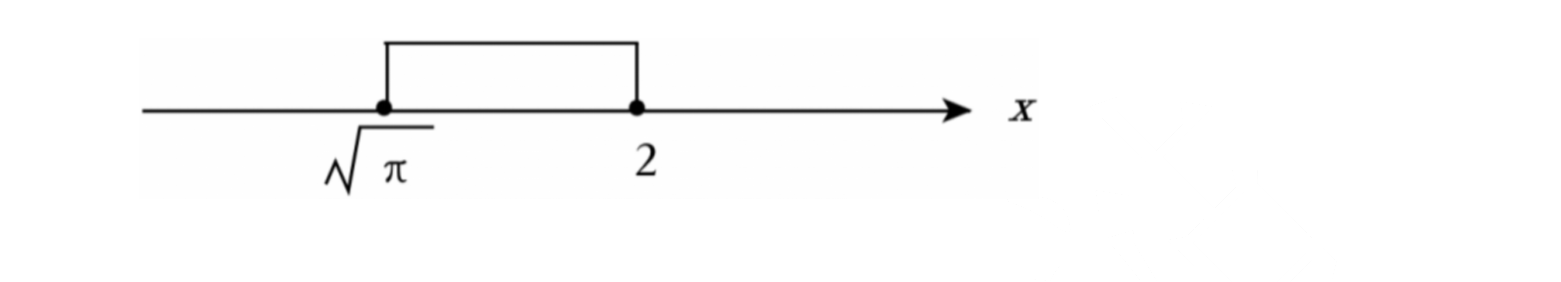
\includegraphics[width=0.72\textwidth]{figures/gao74_q8_numline.png}
\end{center}
\step{所以数形结合得所求集为 $[\sqrt\pi,2]$.}
\solend
\fi

\item 已知集合 $A=\{x\mid(a-1)x^2+3x-3=0,\,x\in\R\}$ 有且仅有一个真子集，则实数 $a=$\blankline[4.4em].

\ifanswer
\solbegin
\step{因为集合 $A=\{x\mid(a-1)x^2+3x-3=0,\,x\in\R\}$ 有且仅有一个真子集，}
\step{所以 $(a-1)x^2+3x-3=0$ 只有一个解，}
\step{所以 $a=1$ 或 $\begin{cases}a\neq1\\ \Delta=3^2-4(a-1)\times(-3)=0\end{cases}$，解得 $a=1$ 或 $a=\dfrac14$.}
\solend
\fi

\item 已知全集 $U=\{(x,y)\mid x,y\in\R\}$，若集合 $A\subseteq U$，且对任意 $(x_1,y_1)\in A$，均存在 $(x_2,y_2)\in A$，使得 $x_1y_2+x_2y_1=0$，则称集合 $A$ 为“对称对点集”. 给出如下集合：

（1）$A=\{(x,y)\mid x,y\in\Z\}$；

（2）$A=\left\{(x,y)\,\middle|\,y=\begin{cases}x+1,&x\geqslant0\\ -x+1,&x<0\end{cases},\ x\in\R,\ x\neq0\right\}$；

（3）$A=\{(x,y)\mid y=x+2,\,x\in\R\}$；

（4）$A=\left\{(x,y)\,\middle|\,y=\dfrac1x,\ x\in\R,\ x\neq0\right\}$.

其中是“对称对点集”的序号为\blankline[4.4em]（写出所有正确的序号）.

\ifanswer
\solbegin
\stepm{(1)}{因为 $0\in\Z$，所以 $(0,0)\in A$.}
\step{对任意 $(x_1,y_1)\in A$，取 $(x_2,y_2)=(0,0)\in A$，}
\step{都有 $x_1\times0+0\times y_1=0$，所以（1）是对称对点集.}
\stepm{(2)}{当 $x_1>0$ 时 $y_1=x_1+1$，取 $x_2=-x_1<0$、$y_2=-x_2+1=x_1+1=y_1$，}
\step{则 $(x_2,y_2)\in A$，且 $x_1y_2+x_2y_1=x_1y_1-x_1y_1=0$；}
\step{当 $x_1<0$ 时同理取 $x_2=-x_1>0$、$y_2=x_2+1=y_1$，}
\step{也有 $(x_2,y_2)\in A$ 且 $x_1y_2+x_2y_1=0$；所以（2）是对称对点集.}
\stepm{(3)}{取 $A$ 中的点 $(-1,1)$. 若存在 $(x_2,y_2)\in A$ 使 $(-1)\cdot y_2+x_2\cdot1=0$，}
\step{则 $y_2=x_2$，但 $A$ 中点的坐标满足 $y=x+2$，两者矛盾，}
\step{所以（3）不是对称对点集.}
\stepm{(4)}{设 $(x_1,y_1)\in A$，则 $x_1\neq0$ 且 $y_1=\dfrac1{x_1}$，}
\step{若存在 $(x_2,y_2)\in A$ 使 $x_1y_2+x_2y_1=0$，}
\step{把 $y_1=\dfrac1{x_1}$、$y_2=\dfrac1{x_2}$（$x_2\neq0$）代入得 $\dfrac{x_1}{x_2}+\dfrac{x_2}{x_1}=0$，即 $x_1^2+x_2^2=0$，}
\step{于是 $x_1=x_2=0$，与 $x_1\neq0$、$x_2\neq0$ 矛盾，所以（4）不是对称对点集.}
\step{故正确的是①②.}
\solend
\fi

\end{enumerate}

\bigsec{二、选择题}

\begin{enumerate}
\setcounter{enumi}{10}

\item “$x>3$”是“$\dfrac{x-1}{x-3}>0$”的\mbox{（\quad）}

\keepwithprev
A. 充分不必要条件\qquad B. 必要不充分条件\qquad C. 充要条件\qquad D. 既不充分也不必要条件

\ifanswer
\solbegin
\step{由 $\dfrac{x-1}{x-3}>0$ 得 $x>3$ 或 $x<1$，故“$x>3$”是“$\dfrac{x-1}{x-3}>0$”的充分不必要条件.}
\step{故选 $A$.}
\solend
\fi

\item 已知 $a,b,c\in\R$，$b>c$，则下列不等式中恒成立的是\mbox{（\quad）}

\keepwithprev
A. $a+b^2>a+c^2$\qquad B. $a^2+b>a^2+c$\qquad C. $ab^2>ac^2$\qquad D. $a^2b>a^2c$

\ifanswer
\solbegin
\step{对于 $A$，取 $b=1,c=-1$，错误；对于 $B$，由不等式的同向可加性得正确；}
\step{对于 $C$，取 $a=1,b=1,c=-2$，错误；对于 $D$，取 $a=0$，错误.}
\step{故选 $B$.}
\solend
\fi

\item 已知关于 $x$ 的不等式 $x^2-2kx+1>0$ 对于一切实数 $x$ 都成立，则实数 $k$ 的取值范围是\mbox{（\quad）}

\keepwithprev
A. $[-1,1]$\qquad B. $(-1,1)$\qquad C. $(-\infty,-1)\cup(1,+\infty)$\qquad D. $\left(-\dfrac12,\dfrac12\right)$

\ifanswer
\solbegin
\step{因为关于 $x$ 的不等式 $x^2-2kx+1>0$ 对于一切实数 $x$ 都成立，}
\step{所以 $\Delta=(-2k)^2-4<0$，即 $4k^2-4<0$，解得 $-1<k<1$，}
\step{所以实数 $k$ 的取值范围是 $(-1,1)$. 故选 $B$.}
\solend
\fi

\item 某种生产设备购买时费用 $100$ 千元，每年的设备管理费 $8$ 千元，这种生产设备的维修费前 $x(x\in\N)$ 年共 $\dfrac{25}{36}x^2+2x$ 千元，问这种生产设备最多使用\mbox{（\quad）}年报废最合算？（即年平均费用最少）

\keepwithprev
A. $13$\qquad B. $10$\qquad C. $15$\qquad D. $12$

\ifanswer
\solbegin
\step{设使用 $x$ 年报废，则总费用 $S(x)=100+8x+\dfrac{25}{36}x^2+2x=\dfrac{25}{36}x^2+10x+100$，}
\step{则年平均费用为 $y=\dfrac{S(x)}x=\dfrac{25x}{36}+\dfrac{100}x+10\geqslant2\sqrt{\dfrac{25x}{36}\cdot\dfrac{100}x}+10=\dfrac{80}3$，}
\step{当且仅当 $\dfrac{25x}{36}=\dfrac{100}x$，即 $x=12$ 时，取等号，}
\step{故当使用 $12$ 年报废，年平均费用最少. 故选 $D$.}
\solend
\fi

\end{enumerate}

\bigsec{三、解答题}

\begin{enumerate}
\setcounter{enumi}{14}

\item （1）设集合 $A=\{x\mid ax-1=0,\,x\in\R\}$，$B=\{x\mid x^2-3x+2=0,\,x\in\R\}$，若 $A\cap B\neq\varnothing$，求实数 $a$ 的取值范围；

（2）已知一元二次方程 $x^2-mx+m+1=0$ 的两个不等实根为 $x_1$、$x_2$，且 $x_1^2+x_2^2=1$，求实数 $m$ 的值.

\ifanswer
\solbegin
\stepm{(1)}{$B=\{x\mid x^2-3x+2=0,\,x\in\R\}=\{1,2\}$，}
\step{①当 $a=0$ 时，方程 $0\cdot x-1=0$ 无解，$A=\varnothing$，$A\cap B=\varnothing$，不符合题意；}
\step{②当 $a\neq0$ 时，$A=\left\{\dfrac1a\right\}$. $A\cap B\neq\varnothing$，}
\step{则 $\dfrac1a\in B$，即 $\dfrac1a=1$ 或 $\dfrac1a=2$，解得 $a=1$ 或 $\dfrac12$；}
\stepm{(2)}{方程 $x^2-mx+m+1=0$ 有两个不等实根，}
\step{则 $\Delta=m^2-4(m+1)>0$，解得 $m>2+2\sqrt2$ 或 $m<2-2\sqrt2$，}
\step{由韦达定理得 $x_1+x_2=m$，$x_1x_2=m+1$，$x_1^2+x_2^2=1$，}
\step{则 $(x_1+x_2)^2-2x_1x_2=m^2-2(m+1)=1$，解得 $m=-1$ 或 $m=3$（舍去），}
\step{综上所述，$m=-1$.}
\solend
\fi

\ansspace

\item 设全集为 $\R$，已知集合 $A=\{x\mid|x-1|\leqslant3,\,x\in\R\}$，

$B=\{x\mid x^2-2mx+(m-3)(m+3)\leqslant0,\,x\in\R\}$.

（1）若 $A\cap B=[0,4]$，求实数 $m$ 的值；

（2）若 $A\cap\overline{B}=A$，求实数 $m$ 的取值范围.

\ifanswer
\solbegin
\stepm{(1)}{$A=\{x\mid|x-1|\leqslant3\}=\{x\mid-2\leqslant x\leqslant4\}$，}
\step{$B=\{x\mid x^2-2mx+(m-3)(m+3)\leqslant0\}=\{x\mid m-3\leqslant x\leqslant m+3\}$，}
\step{若 $A\cap B=[0,4]$，则 $m-3=0$，即 $m=3$；}
\stepm{(2)}{若 $A\cap\overline{B}=A$，则 $A\subseteq\overline{B}$，$\overline{B}=\{x\mid x>m+3\text{ 或 }x<m-3\}$，}
\step{所以 $m+3<-2$ 或 $m-3>4$，解得 $m<-5$ 或 $m>7$，}
\step{实数 $m$ 的取值范围为 $\{m\mid m<-5\text{ 或 }m>7\}$.}
\solend
\fi

\ansspace

\item （1）已知 $a$、$b$ 为正实数，若 $a+b>4$，试用反证法证明：$\dfrac{a}{b+2}$ 和 $\dfrac{b}{a+2}$ 中至少有一个\mbox{大于 $\dfrac12$}；

（2）设 $x$、$y$ 为正实数，$m=\sqrt{2x}+\sqrt{2y}$，$n=\sqrt{x^2+5xy+y^2}$，试比较 $m$、$n$ 的大小，并说明理由.

\ifanswer
\solbegin
\stepm{(1)}{假设 $\dfrac{a}{b+2}\leqslant\dfrac12$ 且 $\dfrac{b}{a+2}\leqslant\dfrac12$，}
\step{又由 $a$、$b$ 为正实数，则有 $2a\leqslant b+2$ 且 $2b\leqslant a+2$，}
\step{两式相加，有 $2a+2b\leqslant a+b+4$，变形得 $a+b\leqslant4$，}
\step{与已知 $a+b>4$ 相矛盾，即假设 $\dfrac{a}{b+2}\leqslant\dfrac12$ 且 $\dfrac{b}{a+2}\leqslant\dfrac12$ 不成立，}
\step{故 $\dfrac{a}{b+2}$ 和 $\dfrac{b}{a+2}$ 中至少有一个\mbox{大于 $\dfrac12$}；}
\stepm{(2)}{$m>n$，理由：$x$、$y$ 为正实数，$m=\sqrt{2x}+\sqrt{2y}$，$n=\sqrt{x^2+5xy+y^2}$，}
\step{则 $m^2=(\sqrt{2x}+\sqrt{2y})^2=2x^2+2y^2+4xy$，$n^2=x^2+y^2+5xy$，}
\step{则有 $m^2-n^2=2x^2+2y^2+4xy-x^2-y^2-5xy=x^2+y^2-xy$}
\step{$=\left(x-\dfrac y2\right)^2+\dfrac{3y^2}4$，}
\step{又 $x$、$y$ 为正实数，则 $m^2-n^2>0$，即 $m^2>n^2$，必有 $m>n$，结论成立.}
\solend
\fi

\ansspace

\item 已知集合 $A=\{a_1,a_2,a_3,\cdots,a_n\}$，$a_i$ 为正整数（$i=1,2,\cdots,n$）.

（1）设 $n=3$，$a_1=1$，$a_2=3$，$a_3=9$，$B=\{a_i+a_j\mid1\leqslant i<j\leqslant3,\,i,j\in\N^*\}$，若互不相同的三个实数 $b_1$、$b_2$、$b_3$，满足 $\{b_i+b_j\mid1\leqslant i<j\leqslant3,\,i,j\in\N^*\}=B$，求有序数组 $(b_1,b_2,b_3)$；

（2）设 $n=4$，$C=\{a_1^2,a_2^2,a_3^2,a_4^2\}$，其中 $a_1<a_2<a_3<a_4$，$A\cap C=\{a_1,a_4\}$，且 $a_1+a_4=10$，$A\cup C$ 中所有元素之和为 $124$，求集合 $A$；

（3）设 $n=2$，有 $7$ 个互不相同的集合 $A$ 分别记为 $A_1$、$A_2$、$A_3$、$\cdots$、$A_7$，且 $A_1\cap A_7=\varnothing$、$A_i\cap A_{i+1}=\varnothing\,(i=1,2,3,\cdots,6)$，记 $D=A_1\cup A_2\cup A_3\cup\cdots\cup A_7$，求 $D$ 中元素个数的最小值.

\ifanswer
\solbegin
\stepm{(1)}{$B=\{a_i+a_j\mid1\leqslant i<j\leqslant3,\,i,j\in\N^*\}=\{1+3,1+9,3+9\}=\{4,10,12\}$，}
\step{由题意，不妨设 $b_1<b_2<b_3$，}
\step{则三个数两两之和为 $\begin{cases}b_1+b_2=4\\ b_1+b_3=10\\ b_2+b_3=12\end{cases}$，解得 $\begin{cases}b_1=1\\ b_2=3\\ b_3=9\end{cases}$，}
\step{所以满足条件的有序数组为 $1$，$3$，$9$ 三个数字的全部排列，}
\step{所以有序数组 $(b_1,b_2,b_3)$ 为 $(1,3,9),(1,9,3),(3,1,9),(3,9,1),(9,1,3),(9,3,1)$；}
\stepm{(2)}{因为 $A\cap C=\{a_1,a_4\}$，所以 $a_1\in C$，$a_4\in C$，}
\step{所以 $a_1$ 是集合 $A$ 中某个正整数的平方，}
\step{又因为 $a_1$ 是最小的正整数，所以只能是 $a_1=1$，此时满足 $1=1^2$.}
\step{又 $a_1+a_4=10$，所以 $a_4=9$，所以 $9$ 也是集合 $A$ 中某个正整数的平方，}
\step{因为 $3^2=9$，所以 $3\in A$，则有 $a_2=3$ 或 $a_3=3$.}
\step{若 $a_3=3$，则 $A=\{1,a_2,3,9\}$，$C=\{1^2,a_2^2,3^2,9^2\}=\{1,a_2^2,9,81\}$，}
\step{因为 $a_1<a_2<a_3<a_4$，且 $a_2$ 为正整数，所以只能是 $a_2=2$，}
\step{故 $A=\{1,2,3,9\}$，$C=\{1,4,9,81\}$，$A\cap C=\{1,9\}$，符合题意，}
\step{则 $A\cup C=\{1,2,3,4,9,81\}$，此时 $1+2+3+4+9+81=100\neq124$，}
\step{故 $a_3=3$ 不符合题意，所以只能 $a_2=3$，}
\step{故 $A=\{1,3,a_3,9\}$，$C=\{1^2,3^2,a_3^2,9^2\}$，此时 $A\cup C=\{1,3,a_3,9,a_3^2,81\}$，}
\step{则有 $1+3+a_3+9+a_3^2+81=124$，}
\step{即 $a_3^2+a_3-30=(a_3+6)(a_3-5)=0$，解得正整数 $a_3=5$，}
\step{此时 $A=\{1,3,5,9\}$，$C=\{1,9,25,81\}$，$A\cup C=\{1,3,5,9,25,81\}$，}
\step{满足 $A\cap C=\{1,9\}$，$A\cup C$ 中所有元素之和为 $1+3+5+9+25+81=124$，}
\step{故 $A=\{1,3,5,9\}$；}
\stepm{(3)}{当 $n=2$ 时，每个集合 $A_i(i=1,2,\cdots,7)$ 均为含有 $2$ 个元素的二元集合，}
\step{设 $D$ 中元素个数为 $m$，}
\step{若 $m\leqslant4$，从 $m$ 个元素中最多能得到 $\dfrac{4\times3}2=6$ 个不同二元集合，不足 $7$ 个，}
\step{故 $m\leqslant4$ 不可能.}
\step{若 $m=5$，则有 $\dfrac{5\times4}2=10$ 个不同二元集合，数量超过 $7$ 个，符合要求.}
\step{因为 $A_i\cap A_{i+1}=\varnothing(i=1,2,3,\cdots,6)$，$A_1\cap A_7=\varnothing$，}
\step{即要求 $7$ 个互不相同的二元集合排成环，}
\step{且相邻（含首尾）集合交集为空集.}
\needvspace{12\baselineskip}
\step{假设 $m=5$，不妨设 $A_1(1,2)$、$A_2(3,4)$、$A_3(1,5)$，则：}
\begin{center}
\renewcommand{\arraystretch}{1.9}
\begin{tabular}{|c|c|c|c|c|}
\hline
$A_4(2,3)$ & $A_5(1,4)$ & $A_6(2,5)$ & $A_7(1,3)$ & 与 $A_1$ 矛盾\\
\hline
 &  & $A_6(3,5)$ & $A_7(2,4)$ & 与 $A_1$ 矛盾\\
\hline
 & $A_5(4,5)$ & $A_6(1,3)$ & $A_7(2,5)$ 或 $A_7(2,4)$ & 与 $A_1$ 矛盾\\
\hline
$A_4(2,4)$ & $A_5(1,3)$ & $A_6(2,5)$ & $A_7(1,4)$ & 与 $A_1$ 矛盾\\
\hline
 &  & $A_6(4,5)$ & $A_7(2,3)$ & 与 $A_1$ 矛盾\\
\hline
 & $A_5(3,5)$ & $A_6(1,4)$ & $A_7(2,3)$ 或 $A_7(2,5)$ & 与 $A_1$ 矛盾\\
\hline
\end{tabular}
\end{center}
\step{故 $m=5$ 不可能.}
\step{综上，$m\geqslant6$，取 $D=\{1,2,3,4,5,6\}$，}
\step{令 $A_1=\{1,2\},A_2=\{3,4\},A_3=\{1,5\},A_4=\{2,4\},A_5=\{3,6\},A_6=\{1,4\}$，}
\step{$A_7=\{5,6\}$，此时 $A_1$、$A_2$、$\cdots$、$A_7$ 是 $7$ 个互不相同的二元集合，}
\step{且 $A_1\cap A_2=\varnothing$，$A_2\cap A_3=\varnothing$，$A_3\cap A_4=\varnothing$，$A_4\cap A_5=\varnothing$，}
\step{$A_5\cap A_6=\varnothing$，$A_6\cap A_7=\varnothing$，$A_7\cap A_1=\varnothing$，满足全部条件，}
\step{故 $D$ 中元素个数的最小值为 $6$.}
\solend
\fi

\ansspace*[7]

\end{enumerate}

\end{document}
"
%
% 原始材料：微信公众号“魔都数学加油站”文章，连载“27学年高一74”；
% 原文标题“27学年高一74——2026-2027年上海市宜川中学高一上10月月考”；
% 原文链接：https://mp.weixin.qq.com/s/ymsl2bmkBRY6ZPDiUFCDTA。
% 页面标注发布时间 2026-10-22 21:45（上海）。
% 正文为 9 张 PNG 页（`原图/高一74_宜川中学_10月月考/01..09.png`）：
% 第 1、2、3 页为 4762×6735，其余 6 页为 2560×3620，均按页序读取。
% 9 页全为试卷正文页（卷首标题在第 1 页页顶，卷末第 18 题 (3) 解析止于第 9 页），
% 无封面页、目录页、二维码或宣传页。粉色斜排“魔都数学加油站”为卷面水印，未录入。
%
% 卷首标题：照卷面印作“2026-2027 年宜川中学高一上 10 月月考”（黑体加粗一行）。
% 原卷年份区间用半角连字符，本稿按全稿惯例排 en dash；原卷无副标题。
%
% 篇幅与题号：原卷自第 3 题起编号（第 1、2 题不在本卷内）。填空题 3—10（8 题）、
% 选择题 11—14（4 题）、解答题 15—18（4 题），共 16 题。本稿沿用原节与原题号，
% 只改排为全稿统一的大节样式。
%
% 讲评版：原卷第 3 题只印【答案】（“{(1,1)}”），本稿只给 \ans{}；其余 15 题均印
% 【解析】，用 \solbegin…\solend。四道选择题的作答括号原卷即留空，答案写在解析末句
% “故选 A／B／B／D”，照录在解析内，不另提 \ans{}。
%
% 副标题：原卷未印副标题。本稿按“知识模块”口径标作“集合与常用逻辑用语、不等式”：
% 16 题中集合与常用逻辑用语 7 题（第 3、9、10、15、16、18 题及第 17 题的反证法），
% 不等式 9 题（第 4—8、11—14、17 题），两类均确有分量，故并标。口径同 高一63、高一68—73。
%
% 与原卷的排版差异：
%   ① 原卷每题下直接印【答案】/【解析】，本稿按全稿惯例将答案与解析置于答案版；
%   ② 原卷未印副标题，本稿按“知识模块”口径补出；
%   ③ 原卷填空横线约四个字宽，本稿按全稿惯例统一排 \blankline[4.4em]；
%   ④ 原卷数集记号排斜体 $R$、$Z$、$N$（第 8、9、10、14—18 题），本稿按全稿惯例
%      改用 $\R$、$\Z$、$\N$（同 高一68—73）；第 18 题的正整数集合作 $\N^*$，照录；
%   ⑤ 原卷句末标点多为西文句点，均逐处照录；
%   ⑥ 第 15—18 题的子问原卷印作“（1）…（2）…”，本稿按 高一69—73 成例用行内
%      “（1）（2）（3）”段，解析中的子问标号用 \stepm{(1)}{…}；
%   ⑦ 每道解答题原卷未留作答空白，本稿按全稿惯例加 \ansspace（末题用 \ansspace*）；
%   ⑧ 选择题的作答括号原卷排半角“(    )”，本稿按全稿惯例排 \mbox{（\quad）}；
%      选项行排照原卷——第 11、13 题一行四条，第 12、14 题一行四条；
%   ⑨ 第 9、14、18 题解析中的不等式组／方程组，原卷均排作“{”连接的多行式，
%      本稿按全稿惯例排 cases；
%   ⑩ 第 8 题解析有一幅数轴图：原卷印在【解析】第 2 行之后，题干无“如图”二字。
%      本稿按原卷截图裁取（`figures/gao74_q8_numline.png`，由第 2 页原图裁出、
%      去除粉色水印后转灰度，未放大），放在答案版解析第 2 条之后；
%   ⑪ 第 18 题 (3) 解析中有一张 5 列 6 行的枚举表（原卷无表头、左侧两列留空以表示
%      沿用上格的 $A_4$／$A_5$），本稿照原卷排成同样的空格表，未加表头、未合并单元格。
%
% 原卷笔误/存疑（均照录未改，正文对应处另有 % 注）：
%   ① 第 14 题题干“维修费前 $x(x\in N)$ 年共 $\dfrac{25}{36}x^2+2x$ 千元”中的
%      $N$ 原卷排斜体，按全稿惯例改 $\N$，含义不变；
%   ② 第 18 题 (3) 的枚举表第 1—3 行与第 4—6 行分属“$A_5(1,4)$”“$A_5(1,3)$”两种
%      情形，原卷只在首行重复写 $A_4$、$A_5$，其余留空；本稿照录留空，未补字。
%
% 行数核对：逐题数 \step/\stepm 条数与原卷【解析】印刷行数，15 题逐一相符，
% 合计 104 条 / 104 行（Q4：1；Q5：2；Q6：3；Q7：3；Q8：3；Q9：3；Q10：15；
% Q11：2；Q12：3；Q13：3；Q14：4；Q15：9；Q16：6；Q17：10；Q18：37）。
% 另第 3 题只印【答案】，提 \ans{}，不计入 \step 账。
%
% 插图：第 8 题解析的数轴图，见上⑩；全卷题干无其他配图。
%
\documentclass[a4paper,11pt]{article}
\usepackage{common}

\begin{document}

\examtitlest[3]{2026--2027 年宜川中学高一上 10 月月考}{集合与常用逻辑用语、不等式}

\bigsec{一、填空题}

\begin{enumerate}
\setcounter{enumi}{2}

\item 已知集合 $A=\{(x,y)\mid y=x\}$，集合 $B=\{(x,y)\mid y=2-x\}$，则 $A\cap B=$\blankline[4.4em].

\ifanswer
\ans{$\{(1,1)\}$}
\fi

\item 已知 $a=\log_3 2$，$b=\log_3 8$，则 $3^{2a-b}=$\blankline[4.4em].

\ifanswer
\solbegin
\step{由 $a=\log_3 2$，$b=\log_3 8$，得 $3^a=2$，$3^b=8$，则 $3^{2a-b}=\dfrac{(3^a)^2}{3^b}=\dfrac48=\dfrac12$.}
\solend
\fi

\item 已知等式 $2x^2+3x+5=a(2x+1)(x+1)+c$ 恒成立，则实数 $c=$\blankline[4.4em].

\ifanswer
\solbegin
\step{$2x^2+3x+5=a(2x+1)(x+1)+c=2ax^2+3ax+a+c$，}
\step{则 $\begin{cases}2a=2\\ 3a=3\\ a+c=5\end{cases}$，解得 $c=4$.}
\solend
\fi

\item 已知 $x>0$，$y>0$，且 $\dfrac9x+\dfrac1y=1$，则 $x\cdot y$ 的最小值是\blankline[4.4em].

\ifanswer
\solbegin
\step{$x>0$，$y>0$，且 $1=\dfrac9x+\dfrac1y\geqslant2\sqrt{\dfrac9{xy}}$，}
\step{当且仅当 $x=9y$，即 $y=2$，$x=18$ 时取等号，所以 $xy\geqslant36$，}
\step{则 $x\cdot y$ 的最小值为 $36$.}
\solend
\fi

\item 已知关于 $x$ 的不等式 $x^2+bx+c>0$（$b$、$c$ 为实数）的解集为 $(-\infty,-2)\cup(3,+\infty)$，则不等式 $cx^2-bx+1\leqslant0$ 的解集为\blankline[4.4em].

\ifanswer
\solbegin
\step{由已知得 $-2$、$3$ 为方程 $x^2+bx+c=0$ 的根，所以 $-2+3=-b$，$-2\times3=c$，}
\step{即 $b=-1$，$c=-6$，所以不等式 $cx^2-bx+1\leqslant0$ 可变形为 $-6x^2+x+1\leqslant0$，}
\step{即 $6x^2-x-1\geqslant0$，解得 $x\leqslant-\dfrac13$ 或 $x\geqslant\dfrac12$，所以解集为 $\left(-\infty,-\dfrac13\right]\cup\left[\dfrac12,+\infty\right)$.}
\solend
\fi

\item 设 $x\in\R$，则方程 $|x-2|+|\sqrt\pi-x|=2-\sqrt\pi$ 的解集为\blankline[4.4em].

\ifanswer
\solbegin
\step{因为方程 $|x-2|+|\sqrt\pi-x|=2-\sqrt\pi$ 可化为 $|x-2|+|x-\sqrt\pi|=2-\sqrt\pi$，}
\needvspace{8\baselineskip}
\step{其表示数轴上实数 $x$ 到 $\sqrt\pi$ 与 $2$ 的距离之和等于 $2-\sqrt\pi$，如图：}
\begin{center}
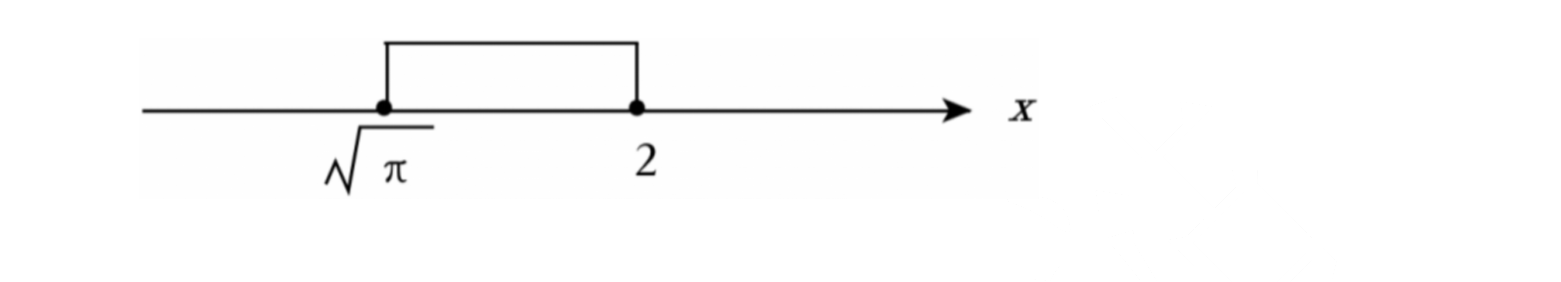
\includegraphics[width=0.72\textwidth]{figures/gao74_q8_numline.png}
\end{center}
\step{所以数形结合得所求集为 $[\sqrt\pi,2]$.}
\solend
\fi

\item 已知集合 $A=\{x\mid(a-1)x^2+3x-3=0,\,x\in\R\}$ 有且仅有一个真子集，则实数 $a=$\blankline[4.4em].

\ifanswer
\solbegin
\step{因为集合 $A=\{x\mid(a-1)x^2+3x-3=0,\,x\in\R\}$ 有且仅有一个真子集，}
\step{所以 $(a-1)x^2+3x-3=0$ 只有一个解，}
\step{所以 $a=1$ 或 $\begin{cases}a\neq1\\ \Delta=3^2-4(a-1)\times(-3)=0\end{cases}$，解得 $a=1$ 或 $a=\dfrac14$.}
\solend
\fi

\item 已知全集 $U=\{(x,y)\mid x,y\in\R\}$，若集合 $A\subseteq U$，且对任意 $(x_1,y_1)\in A$，均存在 $(x_2,y_2)\in A$，使得 $x_1y_2+x_2y_1=0$，则称集合 $A$ 为“对称对点集”. 给出如下集合：

（1）$A=\{(x,y)\mid x,y\in\Z\}$；

（2）$A=\left\{(x,y)\,\middle|\,y=\begin{cases}x+1,&x\geqslant0\\ -x+1,&x<0\end{cases},\ x\in\R,\ x\neq0\right\}$；

（3）$A=\{(x,y)\mid y=x+2,\,x\in\R\}$；

（4）$A=\left\{(x,y)\,\middle|\,y=\dfrac1x,\ x\in\R,\ x\neq0\right\}$.

其中是“对称对点集”的序号为\blankline[4.4em]（写出所有正确的序号）.

\ifanswer
\solbegin
\stepm{(1)}{因为 $0\in\Z$，所以 $(0,0)\in A$.}
\step{对任意 $(x_1,y_1)\in A$，取 $(x_2,y_2)=(0,0)\in A$，}
\step{都有 $x_1\times0+0\times y_1=0$，所以（1）是对称对点集.}
\stepm{(2)}{当 $x_1>0$ 时 $y_1=x_1+1$，取 $x_2=-x_1<0$、$y_2=-x_2+1=x_1+1=y_1$，}
\step{则 $(x_2,y_2)\in A$，且 $x_1y_2+x_2y_1=x_1y_1-x_1y_1=0$；}
\step{当 $x_1<0$ 时同理取 $x_2=-x_1>0$、$y_2=x_2+1=y_1$，}
\step{也有 $(x_2,y_2)\in A$ 且 $x_1y_2+x_2y_1=0$；所以（2）是对称对点集.}
\stepm{(3)}{取 $A$ 中的点 $(-1,1)$. 若存在 $(x_2,y_2)\in A$ 使 $(-1)\cdot y_2+x_2\cdot1=0$，}
\step{则 $y_2=x_2$，但 $A$ 中点的坐标满足 $y=x+2$，两者矛盾，}
\step{所以（3）不是对称对点集.}
\stepm{(4)}{设 $(x_1,y_1)\in A$，则 $x_1\neq0$ 且 $y_1=\dfrac1{x_1}$，}
\step{若存在 $(x_2,y_2)\in A$ 使 $x_1y_2+x_2y_1=0$，}
\step{把 $y_1=\dfrac1{x_1}$、$y_2=\dfrac1{x_2}$（$x_2\neq0$）代入得 $\dfrac{x_1}{x_2}+\dfrac{x_2}{x_1}=0$，即 $x_1^2+x_2^2=0$，}
\step{于是 $x_1=x_2=0$，与 $x_1\neq0$、$x_2\neq0$ 矛盾，所以（4）不是对称对点集.}
\step{故正确的是①②.}
\solend
\fi

\end{enumerate}

\bigsec{二、选择题}

\begin{enumerate}
\setcounter{enumi}{10}

\item “$x>3$”是“$\dfrac{x-1}{x-3}>0$”的\mbox{（\quad）}

\keepwithprev
A. 充分不必要条件\qquad B. 必要不充分条件\qquad C. 充要条件\qquad D. 既不充分也不必要条件

\ifanswer
\solbegin
\step{由 $\dfrac{x-1}{x-3}>0$ 得 $x>3$ 或 $x<1$，故“$x>3$”是“$\dfrac{x-1}{x-3}>0$”的充分不必要条件.}
\step{故选 $A$.}
\solend
\fi

\item 已知 $a,b,c\in\R$，$b>c$，则下列不等式中恒成立的是\mbox{（\quad）}

\keepwithprev
A. $a+b^2>a+c^2$\qquad B. $a^2+b>a^2+c$\qquad C. $ab^2>ac^2$\qquad D. $a^2b>a^2c$

\ifanswer
\solbegin
\step{对于 $A$，取 $b=1,c=-1$，错误；对于 $B$，由不等式的同向可加性得正确；}
\step{对于 $C$，取 $a=1,b=1,c=-2$，错误；对于 $D$，取 $a=0$，错误.}
\step{故选 $B$.}
\solend
\fi

\item 已知关于 $x$ 的不等式 $x^2-2kx+1>0$ 对于一切实数 $x$ 都成立，则实数 $k$ 的取值范围是\mbox{（\quad）}

\keepwithprev
A. $[-1,1]$\qquad B. $(-1,1)$\qquad C. $(-\infty,-1)\cup(1,+\infty)$\qquad D. $\left(-\dfrac12,\dfrac12\right)$

\ifanswer
\solbegin
\step{因为关于 $x$ 的不等式 $x^2-2kx+1>0$ 对于一切实数 $x$ 都成立，}
\step{所以 $\Delta=(-2k)^2-4<0$，即 $4k^2-4<0$，解得 $-1<k<1$，}
\step{所以实数 $k$ 的取值范围是 $(-1,1)$. 故选 $B$.}
\solend
\fi

\item 某种生产设备购买时费用 $100$ 千元，每年的设备管理费 $8$ 千元，这种生产设备的维修费前 $x(x\in\N)$ 年共 $\dfrac{25}{36}x^2+2x$ 千元，问这种生产设备最多使用\mbox{（\quad）}年报废最合算？（即年平均费用最少）

\keepwithprev
A. $13$\qquad B. $10$\qquad C. $15$\qquad D. $12$

\ifanswer
\solbegin
\step{设使用 $x$ 年报废，则总费用 $S(x)=100+8x+\dfrac{25}{36}x^2+2x=\dfrac{25}{36}x^2+10x+100$，}
\step{则年平均费用为 $y=\dfrac{S(x)}x=\dfrac{25x}{36}+\dfrac{100}x+10\geqslant2\sqrt{\dfrac{25x}{36}\cdot\dfrac{100}x}+10=\dfrac{80}3$，}
\step{当且仅当 $\dfrac{25x}{36}=\dfrac{100}x$，即 $x=12$ 时，取等号，}
\step{故当使用 $12$ 年报废，年平均费用最少. 故选 $D$.}
\solend
\fi

\end{enumerate}

\bigsec{三、解答题}

\begin{enumerate}
\setcounter{enumi}{14}

\item （1）设集合 $A=\{x\mid ax-1=0,\,x\in\R\}$，$B=\{x\mid x^2-3x+2=0,\,x\in\R\}$，若 $A\cap B\neq\varnothing$，求实数 $a$ 的取值范围；

（2）已知一元二次方程 $x^2-mx+m+1=0$ 的两个不等实根为 $x_1$、$x_2$，且 $x_1^2+x_2^2=1$，求实数 $m$ 的值.

\ifanswer
\solbegin
\stepm{(1)}{$B=\{x\mid x^2-3x+2=0,\,x\in\R\}=\{1,2\}$，}
\step{①当 $a=0$ 时，方程 $0\cdot x-1=0$ 无解，$A=\varnothing$，$A\cap B=\varnothing$，不符合题意；}
\step{②当 $a\neq0$ 时，$A=\left\{\dfrac1a\right\}$. $A\cap B\neq\varnothing$，}
\step{则 $\dfrac1a\in B$，即 $\dfrac1a=1$ 或 $\dfrac1a=2$，解得 $a=1$ 或 $\dfrac12$；}
\stepm{(2)}{方程 $x^2-mx+m+1=0$ 有两个不等实根，}
\step{则 $\Delta=m^2-4(m+1)>0$，解得 $m>2+2\sqrt2$ 或 $m<2-2\sqrt2$，}
\step{由韦达定理得 $x_1+x_2=m$，$x_1x_2=m+1$，$x_1^2+x_2^2=1$，}
\step{则 $(x_1+x_2)^2-2x_1x_2=m^2-2(m+1)=1$，解得 $m=-1$ 或 $m=3$（舍去），}
\step{综上所述，$m=-1$.}
\solend
\fi

\ansspace

\item 设全集为 $\R$，已知集合 $A=\{x\mid|x-1|\leqslant3,\,x\in\R\}$，

$B=\{x\mid x^2-2mx+(m-3)(m+3)\leqslant0,\,x\in\R\}$.

（1）若 $A\cap B=[0,4]$，求实数 $m$ 的值；

（2）若 $A\cap\overline{B}=A$，求实数 $m$ 的取值范围.

\ifanswer
\solbegin
\stepm{(1)}{$A=\{x\mid|x-1|\leqslant3\}=\{x\mid-2\leqslant x\leqslant4\}$，}
\step{$B=\{x\mid x^2-2mx+(m-3)(m+3)\leqslant0\}=\{x\mid m-3\leqslant x\leqslant m+3\}$，}
\step{若 $A\cap B=[0,4]$，则 $m-3=0$，即 $m=3$；}
\stepm{(2)}{若 $A\cap\overline{B}=A$，则 $A\subseteq\overline{B}$，$\overline{B}=\{x\mid x>m+3\text{ 或 }x<m-3\}$，}
\step{所以 $m+3<-2$ 或 $m-3>4$，解得 $m<-5$ 或 $m>7$，}
\step{实数 $m$ 的取值范围为 $\{m\mid m<-5\text{ 或 }m>7\}$.}
\solend
\fi

\ansspace

\item （1）已知 $a$、$b$ 为正实数，若 $a+b>4$，试用反证法证明：$\dfrac{a}{b+2}$ 和 $\dfrac{b}{a+2}$ 中至少有一个\mbox{大于 $\dfrac12$}；

（2）设 $x$、$y$ 为正实数，$m=\sqrt{2x}+\sqrt{2y}$，$n=\sqrt{x^2+5xy+y^2}$，试比较 $m$、$n$ 的大小，并说明理由.

\ifanswer
\solbegin
\stepm{(1)}{假设 $\dfrac{a}{b+2}\leqslant\dfrac12$ 且 $\dfrac{b}{a+2}\leqslant\dfrac12$，}
\step{又由 $a$、$b$ 为正实数，则有 $2a\leqslant b+2$ 且 $2b\leqslant a+2$，}
\step{两式相加，有 $2a+2b\leqslant a+b+4$，变形得 $a+b\leqslant4$，}
\step{与已知 $a+b>4$ 相矛盾，即假设 $\dfrac{a}{b+2}\leqslant\dfrac12$ 且 $\dfrac{b}{a+2}\leqslant\dfrac12$ 不成立，}
\step{故 $\dfrac{a}{b+2}$ 和 $\dfrac{b}{a+2}$ 中至少有一个\mbox{大于 $\dfrac12$}；}
\stepm{(2)}{$m>n$，理由：$x$、$y$ 为正实数，$m=\sqrt{2x}+\sqrt{2y}$，$n=\sqrt{x^2+5xy+y^2}$，}
\step{则 $m^2=(\sqrt{2x}+\sqrt{2y})^2=2x^2+2y^2+4xy$，$n^2=x^2+y^2+5xy$，}
\step{则有 $m^2-n^2=2x^2+2y^2+4xy-x^2-y^2-5xy=x^2+y^2-xy$}
\step{$=\left(x-\dfrac y2\right)^2+\dfrac{3y^2}4$，}
\step{又 $x$、$y$ 为正实数，则 $m^2-n^2>0$，即 $m^2>n^2$，必有 $m>n$，结论成立.}
\solend
\fi

\ansspace

\item 已知集合 $A=\{a_1,a_2,a_3,\cdots,a_n\}$，$a_i$ 为正整数（$i=1,2,\cdots,n$）.

（1）设 $n=3$，$a_1=1$，$a_2=3$，$a_3=9$，$B=\{a_i+a_j\mid1\leqslant i<j\leqslant3,\,i,j\in\N^*\}$，若互不相同的三个实数 $b_1$、$b_2$、$b_3$，满足 $\{b_i+b_j\mid1\leqslant i<j\leqslant3,\,i,j\in\N^*\}=B$，求有序数组 $(b_1,b_2,b_3)$；

（2）设 $n=4$，$C=\{a_1^2,a_2^2,a_3^2,a_4^2\}$，其中 $a_1<a_2<a_3<a_4$，$A\cap C=\{a_1,a_4\}$，且 $a_1+a_4=10$，$A\cup C$ 中所有元素之和为 $124$，求集合 $A$；

（3）设 $n=2$，有 $7$ 个互不相同的集合 $A$ 分别记为 $A_1$、$A_2$、$A_3$、$\cdots$、$A_7$，且 $A_1\cap A_7=\varnothing$、$A_i\cap A_{i+1}=\varnothing\,(i=1,2,3,\cdots,6)$，记 $D=A_1\cup A_2\cup A_3\cup\cdots\cup A_7$，求 $D$ 中元素个数的最小值.

\ifanswer
\solbegin
\stepm{(1)}{$B=\{a_i+a_j\mid1\leqslant i<j\leqslant3,\,i,j\in\N^*\}=\{1+3,1+9,3+9\}=\{4,10,12\}$，}
\step{由题意，不妨设 $b_1<b_2<b_3$，}
\step{则三个数两两之和为 $\begin{cases}b_1+b_2=4\\ b_1+b_3=10\\ b_2+b_3=12\end{cases}$，解得 $\begin{cases}b_1=1\\ b_2=3\\ b_3=9\end{cases}$，}
\step{所以满足条件的有序数组为 $1$，$3$，$9$ 三个数字的全部排列，}
\step{所以有序数组 $(b_1,b_2,b_3)$ 为 $(1,3,9),(1,9,3),(3,1,9),(3,9,1),(9,1,3),(9,3,1)$；}
\stepm{(2)}{因为 $A\cap C=\{a_1,a_4\}$，所以 $a_1\in C$，$a_4\in C$，}
\step{所以 $a_1$ 是集合 $A$ 中某个正整数的平方，}
\step{又因为 $a_1$ 是最小的正整数，所以只能是 $a_1=1$，此时满足 $1=1^2$.}
\step{又 $a_1+a_4=10$，所以 $a_4=9$，所以 $9$ 也是集合 $A$ 中某个正整数的平方，}
\step{因为 $3^2=9$，所以 $3\in A$，则有 $a_2=3$ 或 $a_3=3$.}
\step{若 $a_3=3$，则 $A=\{1,a_2,3,9\}$，$C=\{1^2,a_2^2,3^2,9^2\}=\{1,a_2^2,9,81\}$，}
\step{因为 $a_1<a_2<a_3<a_4$，且 $a_2$ 为正整数，所以只能是 $a_2=2$，}
\step{故 $A=\{1,2,3,9\}$，$C=\{1,4,9,81\}$，$A\cap C=\{1,9\}$，符合题意，}
\step{则 $A\cup C=\{1,2,3,4,9,81\}$，此时 $1+2+3+4+9+81=100\neq124$，}
\step{故 $a_3=3$ 不符合题意，所以只能 $a_2=3$，}
\step{故 $A=\{1,3,a_3,9\}$，$C=\{1^2,3^2,a_3^2,9^2\}$，此时 $A\cup C=\{1,3,a_3,9,a_3^2,81\}$，}
\step{则有 $1+3+a_3+9+a_3^2+81=124$，}
\step{即 $a_3^2+a_3-30=(a_3+6)(a_3-5)=0$，解得正整数 $a_3=5$，}
\step{此时 $A=\{1,3,5,9\}$，$C=\{1,9,25,81\}$，$A\cup C=\{1,3,5,9,25,81\}$，}
\step{满足 $A\cap C=\{1,9\}$，$A\cup C$ 中所有元素之和为 $1+3+5+9+25+81=124$，}
\step{故 $A=\{1,3,5,9\}$；}
\stepm{(3)}{当 $n=2$ 时，每个集合 $A_i(i=1,2,\cdots,7)$ 均为含有 $2$ 个元素的二元集合，}
\step{设 $D$ 中元素个数为 $m$，}
\step{若 $m\leqslant4$，从 $m$ 个元素中最多能得到 $\dfrac{4\times3}2=6$ 个不同二元集合，不足 $7$ 个，}
\step{故 $m\leqslant4$ 不可能.}
\step{若 $m=5$，则有 $\dfrac{5\times4}2=10$ 个不同二元集合，数量超过 $7$ 个，符合要求.}
\step{因为 $A_i\cap A_{i+1}=\varnothing(i=1,2,3,\cdots,6)$，$A_1\cap A_7=\varnothing$，}
\step{即要求 $7$ 个互不相同的二元集合排成环，}
\step{且相邻（含首尾）集合交集为空集.}
\needvspace{12\baselineskip}
\step{假设 $m=5$，不妨设 $A_1(1,2)$、$A_2(3,4)$、$A_3(1,5)$，则：}
\begin{center}
\renewcommand{\arraystretch}{1.9}
\begin{tabular}{|c|c|c|c|c|}
\hline
$A_4(2,3)$ & $A_5(1,4)$ & $A_6(2,5)$ & $A_7(1,3)$ & 与 $A_1$ 矛盾\\
\hline
 &  & $A_6(3,5)$ & $A_7(2,4)$ & 与 $A_1$ 矛盾\\
\hline
 & $A_5(4,5)$ & $A_6(1,3)$ & $A_7(2,5)$ 或 $A_7(2,4)$ & 与 $A_1$ 矛盾\\
\hline
$A_4(2,4)$ & $A_5(1,3)$ & $A_6(2,5)$ & $A_7(1,4)$ & 与 $A_1$ 矛盾\\
\hline
 &  & $A_6(4,5)$ & $A_7(2,3)$ & 与 $A_1$ 矛盾\\
\hline
 & $A_5(3,5)$ & $A_6(1,4)$ & $A_7(2,3)$ 或 $A_7(2,5)$ & 与 $A_1$ 矛盾\\
\hline
\end{tabular}
\end{center}
\step{故 $m=5$ 不可能.}
\step{综上，$m\geqslant6$，取 $D=\{1,2,3,4,5,6\}$，}
\step{令 $A_1=\{1,2\},A_2=\{3,4\},A_3=\{1,5\},A_4=\{2,4\},A_5=\{3,6\},A_6=\{1,4\}$，}
\step{$A_7=\{5,6\}$，此时 $A_1$、$A_2$、$\cdots$、$A_7$ 是 $7$ 个互不相同的二元集合，}
\step{且 $A_1\cap A_2=\varnothing$，$A_2\cap A_3=\varnothing$，$A_3\cap A_4=\varnothing$，$A_4\cap A_5=\varnothing$，}
\step{$A_5\cap A_6=\varnothing$，$A_6\cap A_7=\varnothing$，$A_7\cap A_1=\varnothing$，满足全部条件，}
\step{故 $D$ 中元素个数的最小值为 $6$.}
\solend
\fi

\ansspace*[7]

\end{enumerate}

\end{document}
